%\pdfoutput=1
% Uncomment line above if submitting to arXiv and using pdflatex

% $Id: main.tex 97873 2016-09-08 18:28:41Z michaelt $
% ============================================================================
% Purpose: Template for LHCb documents
% Authors: Tomasz Skwarnicki, Roger Forty, Ulrik Egede
% Created on: 2010-09-24
% ============================================================================
\documentclass[12pt,a4paper]{article}
%%\documentclass[12pt,letter]{article}
% For two column text, add "twocolumn" as an option to the document
% class. Also uncomment the two "onecolumn" and "twocolumn" lines
% around the title page below.

% Variables that controls behaviour
\usepackage{ifthen} % for conditional statements
\newboolean{pdflatex}
\setboolean{pdflatex}{true} % False for eps figures 

\newboolean{articletitles}
\setboolean{articletitles}{true} % False removes titles in references

\newboolean{uprightparticles}
\setboolean{uprightparticles}{false} %True for upright particle symbols

\newboolean{inbibliography}
\setboolean{inbibliography}{false} %True once you enter the bibliography


\newcommand{\phs}{\ensuremath{\Phi_4}}  %% phase space
\newcommand{\phsd}{\ensuremath{\phi_4}} %% phase space density
\newcommand{\dphs}{\ensuremath{\mathrm{d}\phs}}  

\newcommand{\phsPoint}{\ensuremath{\mathbf{x}}}
\newcommand{\dphsPoint}{\ensuremath{\mathrm{d}^5x}}
\newcommand{\phsPointCP}{\ensuremath{\overline{\mathbf{x}}}}
\newcommand{\dphsPointCP}{\ensuremath{\mathrm{d}^5\overline{x}}}

\newcommand{\cleoc}{{C}{L}{E}{O}{-}{c}}

\newcommand{\prt}[1]{\ensuremath{#1}} %% for particle names
\newcommand{\DDbar}{\prt{D\overline{D}}}
\newcommand{\fourpi}{\prt{\pi^+\pi^-\pi^+\pi^-}}
\newcommand{\KKpipi}{\prt{K^+K^-\pi^+\pi^-}}

\newcommand{\eqnref}[1]{Eq.~\ref{#1}}
\newcommand{\eqnPRDref}[1]{Eq.~(\ref{#1})}
\newcommand{\Eqnref}[1]{Equation~\ref{#1}}
\newcommand{\EqnPRDref}[1]{Equation~(\ref{#1})}
\newcommand{\figref}[1]{Fig.~\ref{#1}}
\newcommand{\Figref}[1]{Figure~\ref{#1}}
\newcommand{\tabref}[1]{Tab.~\ref{#1}}
\newcommand{\Tabref}[1]{Table~\ref{#1}}
\newcommand{\secref}[1]{Sec.~\ref{#1}}
\newcommand{\Secref}[1]{Section~\ref{#1}}
\newcommand{\appref}[1]{App.~\ref{#1}}
\newcommand{\Appref}[1]{Appendix~\ref{#1}}

%%

% THis file contains all the default packages and modifications for
% LHCb formatting

%% %%%%%%%%%%%%%%%%%%
%%  Page formatting
%% %%%%%%%%%%%%%%%%%%
\textheight=230mm
\textwidth=160mm
\oddsidemargin=7mm
\evensidemargin=-10mm
\topmargin=-10mm
\headsep=20mm
\columnsep=5mm
\addtolength{\belowcaptionskip}{0.5em}

\renewcommand{\textfraction}{0.01}
\renewcommand{\floatpagefraction}{0.99}
\renewcommand{\topfraction}{0.9}
\renewcommand{\bottomfraction}{0.9}


\setlength{\hoffset}{-2cm}
\setlength{\voffset}{-2cm}
% Page defaults ...
\topmargin=0.5cm
\oddsidemargin=2.5cm
\textwidth=16cm
\textheight=22cm
% Allow the page size to vary a bit ...
\raggedbottom
% To avoid Latex to be too fussy with line breaking ...
\sloppy

%% %%%%%%%%%%%%%%%%%%%%%%%
%% Packages to be used
%% %%%%%%%%%%%%%%%%%%%%%%% 
\usepackage{microtype}
\usepackage{lineno}  % for line numbering during review
\usepackage{xspace} % To avoid problems with missing or double spaces after
                    % predefined symbold
\usepackage{caption} %these three command get the figure and table captions automatically small
\renewcommand{\captionfont}{\small}
\renewcommand{\captionlabelfont}{\small}

%% Graphics
\usepackage{graphicx}  % to include figures (can also use other packages)
\usepackage{color}
\usepackage{colortbl}
\usepackage{placeins}
\graphicspath{{./figs/}} % Make Latex search fig subdir for figures


%% Math
\usepackage{amsmath} % Adds a large collection of math symbols
\usepackage{amssymb}
\usepackage{amsfonts}
\usepackage{upgreek} % Adds in support for greek letters in roman typeset

%% fix to allow peaceful coexistence of line numbering and
%% mathematical objects
%% http://www.latex-community.org/forum/viewtopic.php?f=5&t=163
%%
\newcommand*\patchAmsMathEnvironmentForLineno[1]{%
\expandafter\let\csname old#1\expandafter\endcsname\csname #1\endcsname
\expandafter\let\csname oldend#1\expandafter\endcsname\csname
end#1\endcsname
 \renewenvironment{#1}%
   {\linenomath\csname old#1\endcsname}%
   {\csname oldend#1\endcsname\endlinenomath}%
}
\newcommand*\patchBothAmsMathEnvironmentsForLineno[1]{%
  \patchAmsMathEnvironmentForLineno{#1}%
  \patchAmsMathEnvironmentForLineno{#1*}%
}
\AtBeginDocument{%
\patchBothAmsMathEnvironmentsForLineno{equation}%
\patchBothAmsMathEnvironmentsForLineno{align}%
\patchBothAmsMathEnvironmentsForLineno{flalign}%
\patchBothAmsMathEnvironmentsForLineno{alignat}%
\patchBothAmsMathEnvironmentsForLineno{gather}%
\patchBothAmsMathEnvironmentsForLineno{multline}%
\patchBothAmsMathEnvironmentsForLineno{eqnarray}%
}

% Get hyperlinks to captions and in references.
% These do not work with revtex. Use "hypertext" as class option instead.
\usepackage{hyperref}    % Hyperlinks in references
\usepackage[all]{hypcap} % Internal hyperlinks to floats.

%%% $Id: lhcb-symbols-def.tex 82618 2015-10-14 14:53:43Z pkoppenb $
%%% ======================================================================
%%% Purpose: Standard LHCb aliases
%%% Author: Originally Ulrik Egede, adapted by Tomasz Skwarnicki for templates,
%%% rewritten by Chris Parkes
%%% Maintainer : Ulrik Egede (2010 - 2012)
%%% Maintainer : Rolf Oldeman (2012 - 2014)
%%% =======================================================================

%%% To use this file outside the normal LHCb document environment, the
%%% following should be added in a preamble (before \begin{document}
%%%
%%%\usepackage{ifthen} 
%%%\newboolean{uprightparticles}
%%%\setboolean{uprightparticles}{false} %Set true for upright particle symbols
\usepackage{xspace} 
\usepackage{upgreek}

%%%%%%%%%%%%%%%%%%%%%%%%%%%%%%%%%%%%%%%%%%%%%%%%%%%%%%%%%%%%
%%%
%%% The following is to ensure that the template automatically can process
%%% this file.
%%%
%%% Add comments with at least three %%% preceding.
%%% Add new sections with one % preceding
%%% Add new subsections with two %% preceding
%%%%%%%%%%%%%%%%%%%%%%%%%%%%%%%%%%%%%%%%%%%%%%%%%%%%%%%%%%%%

%%%%%%%%%%%%%
% Experiments
%%%%%%%%%%%%%
\def\lhcb {\mbox{LHCb}\xspace}
\def\atlas  {\mbox{ATLAS}\xspace}
\def\cms    {\mbox{CMS}\xspace}
\def\alice  {\mbox{ALICE}\xspace}
\def\babar  {\mbox{BaBar}\xspace}
\def\belle  {\mbox{Belle}\xspace}
\def\cleo   {\mbox{CLEO}\xspace}
\def\cdf    {\mbox{CDF}\xspace}
\def\dzero  {\mbox{D0}\xspace}
\def\aleph  {\mbox{ALEPH}\xspace}
\def\delphi {\mbox{DELPHI}\xspace}
\def\opal   {\mbox{OPAL}\xspace}
\def\lthree {\mbox{L3}\xspace}
\def\sld    {\mbox{SLD}\xspace}
%%%\def\argus  {\mbox{ARGUS}\xspace}
%%%\def\uaone  {\mbox{UA1}\xspace}
%%%\def\uatwo  {\mbox{UA2}\xspace}
%%%\def\ux85 {\mbox{UX85}\xspace}
\def\cern {\mbox{CERN}\xspace}
\def\lhc    {\mbox{LHC}\xspace}
\def\lep    {\mbox{LEP}\xspace}
\def\tevatron {Tevatron\xspace}

%% LHCb sub-detectors and sub-systems

%%%\def\pu     {PU\xspace}
\def\velo   {VELO\xspace}
\def\rich   {RICH\xspace}
\def\richone {RICH1\xspace}
\def\richtwo {RICH2\xspace}
\def\ttracker {TT\xspace}
\def\intr   {IT\xspace}
\def\st     {ST\xspace}
\def\ot     {OT\xspace}
%%%\def\Tone   {T1\xspace}
%%%\def\Ttwo   {T2\xspace}
%%%\def\Tthree {T3\xspace}
%%%\def\Mone   {M1\xspace}
%%%\def\Mtwo   {M2\xspace}
%%%\def\Mthree {M3\xspace}
%%%\def\Mfour  {M4\xspace}
%%%\def\Mfive  {M5\xspace}
\def\spd    {SPD\xspace}
\def\presh  {PS\xspace}
\def\ecal   {ECAL\xspace}
\def\hcal   {HCAL\xspace}
%%%\def\bcm    {BCM\xspace}
\def\MagUp {\mbox{\em Mag\kern -0.05em Up}\xspace}
\def\MagDown {\mbox{\em MagDown}\xspace}

\def\ode    {ODE\xspace}
\def\daq    {DAQ\xspace}
\def\tfc    {TFC\xspace}
\def\ecs    {ECS\xspace}
\def\lone   {L0\xspace}
\def\hlt    {HLT\xspace}
\def\hltone {HLT1\xspace}
\def\hlttwo {HLT2\xspace}

%%% Upright (not slanted) Particles

\ifthenelse{\boolean{uprightparticles}}%
{\def\Palpha      {\ensuremath{\upalpha}\xspace}
 \def\Pbeta       {\ensuremath{\upbeta}\xspace}
 \def\Pgamma      {\ensuremath{\upgamma}\xspace}                 
 \def\Pdelta      {\ensuremath{\updelta}\xspace}                 
 \def\Pepsilon    {\ensuremath{\upepsilon}\xspace}                 
 \def\Pvarepsilon {\ensuremath{\upvarepsilon}\xspace}                 
 \def\Pzeta       {\ensuremath{\upzeta}\xspace}                 
 \def\Peta        {\ensuremath{\upeta}\xspace}                 
 \def\Ptheta      {\ensuremath{\uptheta}\xspace}                 
 \def\Pvartheta   {\ensuremath{\upvartheta}\xspace}                 
 \def\Piota       {\ensuremath{\upiota}\xspace}                 
 \def\Pkappa      {\ensuremath{\upkappa}\xspace}                 
 \def\Plambda     {\ensuremath{\uplambda}\xspace}                 
 \def\Pmu         {\ensuremath{\upmu}\xspace}                 
 \def\Pnu         {\ensuremath{\upnu}\xspace}                 
 \def\Pxi         {\ensuremath{\upxi}\xspace}                 
 \def\Ppi         {\ensuremath{\uppi}\xspace}                 
 \def\Pvarpi      {\ensuremath{\upvarpi}\xspace}                 
 \def\Prho        {\ensuremath{\uprho}\xspace}                 
 \def\Pvarrho     {\ensuremath{\upvarrho}\xspace}                 
 \def\Ptau        {\ensuremath{\uptau}\xspace}                 
 \def\Pupsilon    {\ensuremath{\upupsilon}\xspace}                 
 \def\Pphi        {\ensuremath{\upphi}\xspace}                 
 \def\Pvarphi     {\ensuremath{\upvarphi}\xspace}                 
 \def\Pchi        {\ensuremath{\upchi}\xspace}                 
 \def\Ppsi        {\ensuremath{\uppsi}\xspace}                 
 \def\Pomega      {\ensuremath{\upomega}\xspace}                 

 \def\PDelta      {\ensuremath{\Delta}\xspace}                 
 \def\PXi      {\ensuremath{\Xi}\xspace}                 
 \def\PLambda      {\ensuremath{\Lambda}\xspace}                 
 \def\PSigma      {\ensuremath{\Sigma}\xspace}                 
 \def\POmega      {\ensuremath{\Omega}\xspace}                 
 \def\PUpsilon      {\ensuremath{\Upsilon}\xspace}                 
 
 %\mathchardef\Deltares="7101
 %\mathchardef\Xi="7104
 %\mathchardef\Lambda="7103
 %\mathchardef\Sigma="7106
 %\mathchardef\Omega="710A


 \def\PA      {\ensuremath{\mathrm{A}}\xspace}                 
 \def\PB      {\ensuremath{\mathrm{B}}\xspace}                 
 \def\PC      {\ensuremath{\mathrm{C}}\xspace}                 
 \def\PD      {\ensuremath{\mathrm{D}}\xspace}                 
 \def\PE      {\ensuremath{\mathrm{E}}\xspace}                 
 \def\PF      {\ensuremath{\mathrm{F}}\xspace}                 
 \def\PG      {\ensuremath{\mathrm{G}}\xspace}                 
 \def\PH      {\ensuremath{\mathrm{H}}\xspace}                 
 \def\PI      {\ensuremath{\mathrm{I}}\xspace}                 
 \def\PJ      {\ensuremath{\mathrm{J}}\xspace}                 
 \def\PK      {\ensuremath{\mathrm{K}}\xspace}                 
 \def\PL      {\ensuremath{\mathrm{L}}\xspace}                 
 \def\PM      {\ensuremath{\mathrm{M}}\xspace}                 
 \def\PN      {\ensuremath{\mathrm{N}}\xspace}                 
 \def\PO      {\ensuremath{\mathrm{O}}\xspace}                 
 \def\PP      {\ensuremath{\mathrm{P}}\xspace}                 
 \def\PQ      {\ensuremath{\mathrm{Q}}\xspace}                 
 \def\PR      {\ensuremath{\mathrm{R}}\xspace}                 
 \def\PS      {\ensuremath{\mathrm{S}}\xspace}                 
 \def\PT      {\ensuremath{\mathrm{T}}\xspace}                 
 \def\PU      {\ensuremath{\mathrm{U}}\xspace}                 
 \def\PV      {\ensuremath{\mathrm{V}}\xspace}                 
 \def\PW      {\ensuremath{\mathrm{W}}\xspace}                 
 \def\PX      {\ensuremath{\mathrm{X}}\xspace}                 
 \def\PY      {\ensuremath{\mathrm{Y}}\xspace}                 
 \def\PZ      {\ensuremath{\mathrm{Z}}\xspace}                 
 \def\Pa      {\ensuremath{\mathrm{a}}\xspace}                 
 \def\Pb      {\ensuremath{\mathrm{b}}\xspace}                 
 \def\Pc      {\ensuremath{\mathrm{c}}\xspace}                 
 \def\Pd      {\ensuremath{\mathrm{d}}\xspace}                 
 \def\Pe      {\ensuremath{\mathrm{e}}\xspace}                 
 \def\Pf      {\ensuremath{\mathrm{f}}\xspace}                 
 \def\Pg      {\ensuremath{\mathrm{g}}\xspace}                 
 \def\Ph      {\ensuremath{\mathrm{h}}\xspace}                 
 \def\Pi      {\ensuremath{\mathrm{i}}\xspace}                 
 \def\Pj      {\ensuremath{\mathrm{j}}\xspace}                 
 \def\Pk      {\ensuremath{\mathrm{k}}\xspace}                 
 \def\Pl      {\ensuremath{\mathrm{l}}\xspace}                 
 \def\Pm      {\ensuremath{\mathrm{m}}\xspace}                 
 \def\Pn      {\ensuremath{\mathrm{n}}\xspace}                 
 \def\Po      {\ensuremath{\mathrm{o}}\xspace}                 
 \def\Pp      {\ensuremath{\mathrm{p}}\xspace}                 
 \def\Pq      {\ensuremath{\mathrm{q}}\xspace}                 
 \def\Pr      {\ensuremath{\mathrm{r}}\xspace}                 
 \def\Ps      {\ensuremath{\mathrm{s}}\xspace}                 
 \def\Pt      {\ensuremath{\mathrm{t}}\xspace}                 
 \def\Pu      {\ensuremath{\mathrm{u}}\xspace}                 
 \def\Pv      {\ensuremath{\mathrm{v}}\xspace}                 
 \def\Pw      {\ensuremath{\mathrm{w}}\xspace}                 
 \def\Px      {\ensuremath{\mathrm{x}}\xspace}                 
 \def\Py      {\ensuremath{\mathrm{y}}\xspace}                 
 \def\Pz      {\ensuremath{\mathrm{z}}\xspace}                 
}
{\def\Palpha      {\ensuremath{\alpha}\xspace}
 \def\Pbeta       {\ensuremath{\beta}\xspace}
 \def\Pgamma      {\ensuremath{\gamma}\xspace}                 
 \def\Pdelta      {\ensuremath{\delta}\xspace}                 
 \def\Pepsilon    {\ensuremath{\epsilon}\xspace}                 
 \def\Pvarepsilon {\ensuremath{\varepsilon}\xspace}                 
 \def\Pzeta       {\ensuremath{\zeta}\xspace}                 
 \def\Peta        {\ensuremath{\eta}\xspace}                 
 \def\Ptheta      {\ensuremath{\theta}\xspace}                 
 \def\Pvartheta   {\ensuremath{\vartheta}\xspace}                 
 \def\Piota       {\ensuremath{\iota}\xspace}                 
 \def\Pkappa      {\ensuremath{\kappa}\xspace}                 
 \def\Plambda     {\ensuremath{\lambda}\xspace}                 
 \def\Pmu         {\ensuremath{\mu}\xspace}                 
 \def\Pnu         {\ensuremath{\nu}\xspace}                 
 \def\Pxi         {\ensuremath{\xi}\xspace}                 
 \def\Ppi         {\ensuremath{\pi}\xspace}                 
 \def\Pvarpi      {\ensuremath{\varpi}\xspace}                 
 \def\Prho        {\ensuremath{\rho}\xspace}                 
 \def\Pvarrho     {\ensuremath{\varrho}\xspace}                 
 \def\Ptau        {\ensuremath{\tau}\xspace}                 
 \def\Pupsilon    {\ensuremath{\upsilon}\xspace}                 
 \def\Pphi        {\ensuremath{\phi}\xspace}                 
 \def\Pvarphi     {\ensuremath{\varphi}\xspace}                 
 \def\Pchi        {\ensuremath{\chi}\xspace}                 
 \def\Ppsi        {\ensuremath{\psi}\xspace}                 
 \def\Pomega      {\ensuremath{\omega}\xspace}                 
 \mathchardef\PDelta="7101
 \mathchardef\PXi="7104
 \mathchardef\PLambda="7103
 \mathchardef\PSigma="7106
 \mathchardef\POmega="710A
 \mathchardef\PUpsilon="7107
 \def\PA      {\ensuremath{A}\xspace}                 
 \def\PB      {\ensuremath{B}\xspace}                 
 \def\PC      {\ensuremath{C}\xspace}                 
 \def\PD      {\ensuremath{D}\xspace}                 
 \def\PE      {\ensuremath{E}\xspace}                 
 \def\PF      {\ensuremath{F}\xspace}                 
 \def\PG      {\ensuremath{G}\xspace}                 
 \def\PH      {\ensuremath{H}\xspace}                 
 \def\PI      {\ensuremath{I}\xspace}                 
 \def\PJ      {\ensuremath{J}\xspace}                 
 \def\PK      {\ensuremath{K}\xspace}                 
 \def\PL      {\ensuremath{L}\xspace}                 
 \def\PM      {\ensuremath{M}\xspace}                 
 \def\PN      {\ensuremath{N}\xspace}                 
 \def\PO      {\ensuremath{O}\xspace}                 
 \def\PP      {\ensuremath{P}\xspace}                 
 \def\PQ      {\ensuremath{Q}\xspace}                 
 \def\PR      {\ensuremath{R}\xspace}                 
 \def\PS      {\ensuremath{S}\xspace}                 
 \def\PT      {\ensuremath{T}\xspace}                 
 \def\PU      {\ensuremath{U}\xspace}                 
 \def\PV      {\ensuremath{V}\xspace}                 
 \def\PW      {\ensuremath{W}\xspace}                 
 \def\PX      {\ensuremath{X}\xspace}                 
 \def\PY      {\ensuremath{Y}\xspace}                 
 \def\PZ      {\ensuremath{Z}\xspace}                 
 \def\Pa      {\ensuremath{a}\xspace}                 
 \def\Pb      {\ensuremath{b}\xspace}                 
 \def\Pc      {\ensuremath{c}\xspace}                 
 \def\Pd      {\ensuremath{d}\xspace}                 
 \def\Pe      {\ensuremath{e}\xspace}                 
 \def\Pf      {\ensuremath{f}\xspace}                 
 \def\Pg      {\ensuremath{g}\xspace}                 
 \def\Ph      {\ensuremath{h}\xspace}                 
 \def\Pi      {\ensuremath{i}\xspace}                 
 \def\Pj      {\ensuremath{j}\xspace}                 
 \def\Pk      {\ensuremath{k}\xspace}                 
 \def\Pl      {\ensuremath{l}\xspace}                 
 \def\Pm      {\ensuremath{m}\xspace}                 
 \def\Pn      {\ensuremath{n}\xspace}                 
 \def\Po      {\ensuremath{o}\xspace}                 
 \def\Pp      {\ensuremath{p}\xspace}                 
 \def\Pq      {\ensuremath{q}\xspace}                 
 \def\Pr      {\ensuremath{r}\xspace}                 
 \def\Ps      {\ensuremath{s}\xspace}                 
 \def\Pt      {\ensuremath{t}\xspace}                 
 \def\Pu      {\ensuremath{u}\xspace}                 
 \def\Pv      {\ensuremath{v}\xspace}                 
 \def\Pw      {\ensuremath{w}\xspace}                 
 \def\Px      {\ensuremath{x}\xspace}                 
 \def\Py      {\ensuremath{y}\xspace}                 
 \def\Pz      {\ensuremath{z}\xspace}                 
}

%%%%%%%%%%%%%%%%%%%%%%%%%%%%%%%%%%%%%%%%%%%%%%%
% Particles
\makeatletter
\ifcase \@ptsize \relax% 10pt
  \newcommand{\miniscule}{\@setfontsize\miniscule{4}{5}}% \tiny: 5/6
\or% 11pt
  \newcommand{\miniscule}{\@setfontsize\miniscule{5}{6}}% \tiny: 6/7
\or% 12pt
  \newcommand{\miniscule}{\@setfontsize\miniscule{5}{6}}% \tiny: 6/7
\fi
\makeatother


\DeclareRobustCommand{\optbar}[1]{\shortstack{{\miniscule (\rule[.5ex]{1.25em}{.18mm})}
  \\ [-.7ex] $#1$}}


%% Leptons

\let\emi\en
\def\electron   {{\ensuremath{\Pe}}\xspace}
\def\en         {{\ensuremath{\Pe^-}}\xspace}   % electron negative (\em is taken)
\def\ep         {{\ensuremath{\Pe^+}}\xspace}
\def\epm        {{\ensuremath{\Pe^\pm}}\xspace} 
\def\epem       {{\ensuremath{\Pe^+\Pe^-}}\xspace}
%%%\def\ee         {\ensuremath{\Pe^-\Pe^-}\xspace}

\def\muon       {{\ensuremath{\Pmu}}\xspace}
\def\mup        {{\ensuremath{\Pmu^+}}\xspace}
\def\mun        {{\ensuremath{\Pmu^-}}\xspace} % muon negative (\mum is taken)
\def\mumu       {{\ensuremath{\Pmu^+\Pmu^-}}\xspace}

\def\tauon      {{\ensuremath{\Ptau}}\xspace}
\def\taup       {{\ensuremath{\Ptau^+}}\xspace}
\def\taum       {{\ensuremath{\Ptau^-}}\xspace}
\def\tautau     {{\ensuremath{\Ptau^+\Ptau^-}}\xspace}

\def\lepton     {{\ensuremath{\ell}}\xspace}
\def\ellm       {{\ensuremath{\ell^-}}\xspace}
\def\ellp       {{\ensuremath{\ell^+}}\xspace}
%%%\def\ellell     {\ensuremath{\ell^+ \ell^-}\xspace}

\def\neu        {{\ensuremath{\Pnu}}\xspace}
\def\neub       {{\ensuremath{\overline{\Pnu}}}\xspace}
%%%\def\nuenueb    {\ensuremath{\neu\neub}\xspace}
\def\neue       {{\ensuremath{\neu_e}}\xspace}
\def\neueb      {{\ensuremath{\neub_e}}\xspace}
%%%\def\neueneueb  {\ensuremath{\neue\neueb}\xspace}
\def\neum       {{\ensuremath{\neu_\mu}}\xspace}
\def\neumb      {{\ensuremath{\neub_\mu}}\xspace}
%%%\def\neumneumb  {\ensuremath{\neum\neumb}\xspace}
\def\neut       {{\ensuremath{\neu_\tau}}\xspace}
\def\neutb      {{\ensuremath{\neub_\tau}}\xspace}
%%%\def\neutneutb  {\ensuremath{\neut\neutb}\xspace}
\def\neul       {{\ensuremath{\neu_\ell}}\xspace}
\def\neulb      {{\ensuremath{\neub_\ell}}\xspace}
%%%\def\neulneulb  {\ensuremath{\neul\neulb}\xspace}

%% Gauge bosons and scalars

\def\g      {{\ensuremath{\Pgamma}}\xspace}
\def\H      {{\ensuremath{\PH^0}}\xspace}
\def\Hp     {{\ensuremath{\PH^+}}\xspace}
\def\Hm     {{\ensuremath{\PH^-}}\xspace}
\def\Hpm    {{\ensuremath{\PH^\pm}}\xspace}
\def\W      {{\ensuremath{\PW}}\xspace}
\def\Wp     {{\ensuremath{\PW^+}}\xspace}
\def\Wm     {{\ensuremath{\PW^-}}\xspace}
\def\Wpm    {{\ensuremath{\PW^\pm}}\xspace}
\def\Z      {{\ensuremath{\PZ}}\xspace}

%% Quarks

\def\quark     {{\ensuremath{\Pq}}\xspace}
\def\quarkbar  {{\ensuremath{\overline \quark}}\xspace}
\def\qqbar     {{\ensuremath{\quark\quarkbar}}\xspace}
\def\uquark    {{\ensuremath{\Pu}}\xspace}
\def\uquarkbar {{\ensuremath{\overline \uquark}}\xspace}
\def\uubar     {{\ensuremath{\uquark\uquarkbar}}\xspace}
\def\dquark    {{\ensuremath{\Pd}}\xspace}
\def\dquarkbar {{\ensuremath{\overline \dquark}}\xspace}
\def\ddbar     {{\ensuremath{\dquark\dquarkbar}}\xspace}
\def\squark    {{\ensuremath{\Ps}}\xspace}
\def\squarkbar {{\ensuremath{\overline \squark}}\xspace}
\def\ssbar     {{\ensuremath{\squark\squarkbar}}\xspace}
\def\cquark    {{\ensuremath{\Pc}}\xspace}
\def\cquarkbar {{\ensuremath{\overline \cquark}}\xspace}
\def\ccbar     {{\ensuremath{\cquark\cquarkbar}}\xspace}
\def\bquark    {{\ensuremath{\Pb}}\xspace}
\def\bquarkbar {{\ensuremath{\overline \bquark}}\xspace}
\def\bbbar     {{\ensuremath{\bquark\bquarkbar}}\xspace}
\def\tquark    {{\ensuremath{\Pt}}\xspace}
\def\tquarkbar {{\ensuremath{\overline \tquark}}\xspace}
\def\ttbar     {{\ensuremath{\tquark\tquarkbar}}\xspace}

%% Light mesons

\def\hadron {{\ensuremath{\Ph}}\xspace}
\def\pion   {{\ensuremath{\Ppi}}\xspace}
\def\piz    {{\ensuremath{\pion^0}}\xspace}
\def\pizs   {{\ensuremath{\pion^0\mbox\,\mathrm{s}}}\xspace}
\def\pip    {{\ensuremath{\pion^+}}\xspace}
\def\pim    {{\ensuremath{\pion^-}}\xspace}
\def\pipm   {{\ensuremath{\pion^\pm}}\xspace}
\def\pimp   {{\ensuremath{\pion^\mp}}\xspace}

\def\rhomeson {{\ensuremath{\Prho}}\xspace}
\def\rhoz     {{\ensuremath{\rhomeson^0}}\xspace}
\def\rhop     {{\ensuremath{\rhomeson^+}}\xspace}
\def\rhom     {{\ensuremath{\rhomeson^-}}\xspace}
\def\rhopm    {{\ensuremath{\rhomeson^\pm}}\xspace}
\def\rhomp    {{\ensuremath{\rhomeson^\mp}}\xspace}

\def\kaon    {{\ensuremath{\PK}}\xspace}
%%% do NOT use ensuremath here
  \def\Kbar    {{\kern 0.2em\overline{\kern -0.2em \PK}{}}\xspace}
\def\Kb      {{\ensuremath{\Kbar}}\xspace}
\def\KorKbar    {\kern 0.18em\optbar{\kern -0.18em K}{}\xspace}
\def\Kz      {{\ensuremath{\kaon^0}}\xspace}
\def\Kzb     {{\ensuremath{\Kbar{}^0}}\xspace}
\def\Kp      {{\ensuremath{\kaon^+}}\xspace}
\def\Km      {{\ensuremath{\kaon^-}}\xspace}
\def\Kpm     {{\ensuremath{\kaon^\pm}}\xspace}
\def\Kmp     {{\ensuremath{\kaon^\mp}}\xspace}
\def\KS      {{\ensuremath{\kaon^0_{\mathrm{ \scriptscriptstyle S}}}}\xspace}
\def\KL      {{\ensuremath{\kaon^0_{\mathrm{ \scriptscriptstyle L}}}}\xspace}
\def\Kstarz  {{\ensuremath{\kaon^{*0}}}\xspace}
\def\Kstarzb {{\ensuremath{\Kbar{}^{*0}}}\xspace}
\def\Kstar   {{\ensuremath{\kaon^*}}\xspace}
\def\Kstarb  {{\ensuremath{\Kbar{}^*}}\xspace}
\def\Kstarp  {{\ensuremath{\kaon^{*+}}}\xspace}
\def\Kstarm  {{\ensuremath{\kaon^{*-}}}\xspace}
\def\Kstarpm {{\ensuremath{\kaon^{*\pm}}}\xspace}
\def\Kstarmp {{\ensuremath{\kaon^{*\mp}}}\xspace}

\newcommand{\etaz}{\ensuremath{\Peta}\xspace}
\newcommand{\etapr}{\ensuremath{\Peta^{\prime}}\xspace}
\newcommand{\phiz}{\ensuremath{\Pphi}\xspace}
\newcommand{\omegaz}{\ensuremath{\Pomega}\xspace}

%% Heavy mesons

%%% do NOT use ensuremath here
  \def\Dbar    {{\kern 0.2em\overline{\kern -0.2em \PD}{}}\xspace}
\def\D       {{\ensuremath{\PD}}\xspace}
\def\Db      {{\ensuremath{\Dbar}}\xspace}
\def\DorDbar    {\kern 0.18em\optbar{\kern -0.18em D}{}\xspace}
\def\Dz      {{\ensuremath{\D^0}}\xspace}
\def\Dzb     {{\ensuremath{\Dbar{}^0}}\xspace}
\def\Dp      {{\ensuremath{\D^+}}\xspace}
\def\Dm      {{\ensuremath{\D^-}}\xspace}
\def\Dpm     {{\ensuremath{\D^\pm}}\xspace}
\def\Dmp     {{\ensuremath{\D^\mp}}\xspace}
\def\Dstar   {{\ensuremath{\D^*}}\xspace}
\def\Dstarb  {{\ensuremath{\Dbar{}^*}}\xspace}
\def\Dstarz  {{\ensuremath{\D^{*0}}}\xspace}
\def\Dstarzb {{\ensuremath{\Dbar{}^{*0}}}\xspace}
\def\Dstarp  {{\ensuremath{\D^{*+}}}\xspace}
\def\Dstarm  {{\ensuremath{\D^{*-}}}\xspace}
\def\Dstarpm {{\ensuremath{\D^{*\pm}}}\xspace}
\def\Dstarmp {{\ensuremath{\D^{*\mp}}}\xspace}
\def\Ds      {{\ensuremath{\D^+_\squark}}\xspace}
\def\Dsp     {{\ensuremath{\D^+_\squark}}\xspace}
\def\Dsm     {{\ensuremath{\D^-_\squark}}\xspace}
\def\Dspm    {{\ensuremath{\D^{\pm}_\squark}}\xspace}
\def\Dsmp    {{\ensuremath{\D^{\mp}_\squark}}\xspace}
\def\Dss     {{\ensuremath{\D^{*+}_\squark}}\xspace}
\def\Dssp    {{\ensuremath{\D^{*+}_\squark}}\xspace}
\def\Dssm    {{\ensuremath{\D^{*-}_\squark}}\xspace}
\def\Dsspm   {{\ensuremath{\D^{*\pm}_\squark}}\xspace}
\def\Dssmp   {{\ensuremath{\D^{*\mp}_\squark}}\xspace}

\def\B       {{\ensuremath{\PB}}\xspace}
%%% do NOT use ensuremath here
\def\Bbar    {{\ensuremath{\kern 0.18em\overline{\kern -0.18em \PB}{}}}\xspace}
\def\Bb      {{\ensuremath{\Bbar}}\xspace}
\def\BorBbar    {\kern 0.18em\optbar{\kern -0.18em B}{}\xspace}
\def\Bz      {{\ensuremath{\B^0}}\xspace}
\def\Bzb     {{\ensuremath{\Bbar{}^0}}\xspace}
\def\Bu      {{\ensuremath{\B^+}}\xspace}
\def\Bub     {{\ensuremath{\B^-}}\xspace}
\def\Bp      {{\ensuremath{\Bu}}\xspace}
\def\Bm      {{\ensuremath{\Bub}}\xspace}
\def\Bpm     {{\ensuremath{\B^\pm}}\xspace}
\def\Bmp     {{\ensuremath{\B^\mp}}\xspace}
\def\Bd      {{\ensuremath{\B^0}}\xspace}
\def\Bs      {{\ensuremath{\B^0_\squark}}\xspace}
\def\Bsb     {{\ensuremath{\Bbar{}^0_\squark}}\xspace}
\def\Bdb     {{\ensuremath{\Bbar{}^0}}\xspace}
\def\Bc      {{\ensuremath{\B_\cquark^+}}\xspace}
\def\Bcp     {{\ensuremath{\B_\cquark^+}}\xspace}
\def\Bcm     {{\ensuremath{\B_\cquark^-}}\xspace}
\def\Bcpm    {{\ensuremath{\B_\cquark^\pm}}\xspace}

%% Onia

\def\jpsi     {{\ensuremath{{\PJ\mskip -3mu/\mskip -2mu\Ppsi\mskip 2mu}}}\xspace}
\def\psitwos  {{\ensuremath{\Ppsi{(2S)}}}\xspace}
\def\psiprpr  {{\ensuremath{\Ppsi(3770)}}\xspace}
\def\etac     {{\ensuremath{\Peta_\cquark}}\xspace}
\def\chiczero {{\ensuremath{\Pchi_{\cquark 0}}}\xspace}
\def\chicone  {{\ensuremath{\Pchi_{\cquark 1}}}\xspace}
\def\chictwo  {{\ensuremath{\Pchi_{\cquark 2}}}\xspace}
  %\mathchardef\Upsilon="7107
  \def\Y#1S{\ensuremath{\PUpsilon{(#1S)}}\xspace}% no space before {...}!
\def\OneS  {{\Y1S}}
\def\TwoS  {{\Y2S}}
\def\ThreeS{{\Y3S}}
\def\FourS {{\Y4S}}
\def\FiveS {{\Y5S}}

\def\chic  {{\ensuremath{\Pchi_{c}}}\xspace}

%% Baryons

\def\proton      {{\ensuremath{\Pp}}\xspace}
\def\antiproton  {{\ensuremath{\overline \proton}}\xspace}
\def\neutron     {{\ensuremath{\Pn}}\xspace}
\def\antineutron {{\ensuremath{\overline \neutron}}\xspace}
\def\Deltares    {{\ensuremath{\PDelta}}\xspace}
\def\Deltaresbar {{\ensuremath{\overline \Deltares}}\xspace}
\def\Xires       {{\ensuremath{\PXi}}\xspace}
\def\Xiresbar    {{\ensuremath{\overline \Xires}}\xspace}
\def\Lz          {{\ensuremath{\PLambda}}\xspace}
\def\Lbar        {{\ensuremath{\kern 0.1em\overline{\kern -0.1em\PLambda}}}\xspace}
\def\LorLbar    {\kern 0.18em\optbar{\kern -0.18em \PLambda}{}\xspace}
\def\Lambdares   {{\ensuremath{\PLambda}}\xspace}
\def\Lambdaresbar{{\ensuremath{\Lbar}}\xspace}
\def\Sigmares    {{\ensuremath{\PSigma}}\xspace}
\def\Sigmaresbar {{\ensuremath{\overline \Sigmares}}\xspace}
\def\Omegares    {{\ensuremath{\POmega}}\xspace}
\def\Omegaresbar {{\ensuremath{\overline \POmega}}\xspace}

%%% do NOT use ensuremath here
 % \def\Deltabar{\kern 0.25em\overline{\kern -0.25em \Deltares}{}\xspace}
 % \def\Sigbar{\kern 0.2em\overline{\kern -0.2em \Sigma}{}\xspace}
 % \def\Xibar{\kern 0.2em\overline{\kern -0.2em \Xi}{}\xspace}
 % \def\Obar{\kern 0.2em\overline{\kern -0.2em \Omega}{}\xspace}
 % \def\Nbar{\kern 0.2em\overline{\kern -0.2em N}{}\xspace}
 % \def\Xb{\kern 0.2em\overline{\kern -0.2em X}{}\xspace}

\def\Lb      {{\ensuremath{\Lz^0_\bquark}}\xspace}
\def\Lbbar   {{\ensuremath{\Lbar{}^0_\bquark}}\xspace}
\def\Lc      {{\ensuremath{\Lz^+_\cquark}}\xspace}
\def\Lcbar   {{\ensuremath{\Lbar{}^-_\cquark}}\xspace}
\def\Xib     {{\ensuremath{\Xires_\bquark}}\xspace}
\def\Xibz    {{\ensuremath{\Xires^0_\bquark}}\xspace}
\def\Xibm    {{\ensuremath{\Xires^-_\bquark}}\xspace}
\def\Xibbar  {{\ensuremath{\Xiresbar{}_\bquark}}\xspace}
\def\Xibbarz {{\ensuremath{\Xiresbar{}_\bquark^0}}\xspace}
\def\Xibbarp {{\ensuremath{\Xiresbar{}_\bquark^+}}\xspace}
\def\Xic     {{\ensuremath{\Xires_\cquark}}\xspace}
\def\Xicz    {{\ensuremath{\Xires^0_\cquark}}\xspace}
\def\Xicp    {{\ensuremath{\Xires^+_\cquark}}\xspace}
\def\Xicbar  {{\ensuremath{\Xiresbar{}_\cquark}}\xspace}
\def\Xicbarz {{\ensuremath{\Xiresbar{}_\cquark^0}}\xspace}
\def\Xicbarm {{\ensuremath{\Xiresbar{}_\cquark^-}}\xspace}
\def\Omegac    {{\ensuremath{\Omegares^0_\cquark}}\xspace}
\def\Omegacbar {{\ensuremath{\Omegaresbar{}_\cquark^0}}\xspace}
\def\Omegab    {{\ensuremath{\Omegares^-_\bquark}}\xspace}
\def\Omegabbar {{\ensuremath{\Omegaresbar{}_\bquark^+}}\xspace}

%%%%%%%%%%%%%%%%%%
% Physics symbols
%%%%%%%%%%%%%%%%%

%% Decays
\def\BF         {{\ensuremath{\mathcal{B}}}\xspace}
\def\BRvis      {{\ensuremath{\BR_{\mathrm{{vis}}}}}}
\def\BR         {\BF}
\newcommand{\decay}[2]{\ensuremath{#1\!\to #2}\xspace}         % {\Pa}{\Pb \Pc}
\def\ra                 {\ensuremath{\rightarrow}\xspace}
\def\to                 {\ensuremath{\rightarrow}\xspace}

%% Lifetimes
\newcommand{\tauBs}{{\ensuremath{\tau_{\Bs}}}\xspace}
\newcommand{\tauBd}{{\ensuremath{\tau_{\Bd}}}\xspace}
\newcommand{\tauBz}{{\ensuremath{\tau_{\Bz}}}\xspace}
\newcommand{\tauBu}{{\ensuremath{\tau_{\Bp}}}\xspace}
\newcommand{\tauDp}{{\ensuremath{\tau_{\Dp}}}\xspace}
\newcommand{\tauDz}{{\ensuremath{\tau_{\Dz}}}\xspace}
\newcommand{\tauL}{{\ensuremath{\tau_{\mathrm{ L}}}}\xspace}
\newcommand{\tauH}{{\ensuremath{\tau_{\mathrm{ H}}}}\xspace}

%% Masses
\newcommand{\mBd}{{\ensuremath{m_{\Bd}}}\xspace}
\newcommand{\mBp}{{\ensuremath{m_{\Bp}}}\xspace}
\newcommand{\mBs}{{\ensuremath{m_{\Bs}}}\xspace}
\newcommand{\mBc}{{\ensuremath{m_{\Bc}}}\xspace}
\newcommand{\mLb}{{\ensuremath{m_{\Lb}}}\xspace}

%% EW theory, groups
\def\grpsuthree {{\ensuremath{\mathrm{SU}(3)}}\xspace}
\def\grpsutw    {{\ensuremath{\mathrm{SU}(2)}}\xspace}
\def\grpuone    {{\ensuremath{\mathrm{U}(1)}}\xspace}

\def\ssqtw   {{\ensuremath{\sin^{2}\!\theta_{\mathrm{W}}}}\xspace}
\def\csqtw   {{\ensuremath{\cos^{2}\!\theta_{\mathrm{W}}}}\xspace}
\def\stw     {{\ensuremath{\sin\theta_{\mathrm{W}}}}\xspace}
\def\ctw     {{\ensuremath{\cos\theta_{\mathrm{W}}}}\xspace}
\def\ssqtwef {{\ensuremath{{\sin}^{2}\theta_{\mathrm{W}}^{\mathrm{eff}}}}\xspace}
\def\csqtwef {{\ensuremath{{\cos}^{2}\theta_{\mathrm{W}}^{\mathrm{eff}}}}\xspace}
\def\stwef   {{\ensuremath{\sin\theta_{\mathrm{W}}^{\mathrm{eff}}}}\xspace}
\def\ctwef   {{\ensuremath{\cos\theta_{\mathrm{W}}^{\mathrm{eff}}}}\xspace}
\def\gv      {{\ensuremath{g_{\mbox{\tiny V}}}}\xspace}
\def\ga      {{\ensuremath{g_{\mbox{\tiny A}}}}\xspace}

\def\order   {{\ensuremath{\mathcal{O}}}\xspace}
\def\ordalph {{\ensuremath{\mathcal{O}(\alpha)}}\xspace}
\def\ordalsq {{\ensuremath{\mathcal{O}(\alpha^{2})}}\xspace}
\def\ordalcb {{\ensuremath{\mathcal{O}(\alpha^{3})}}\xspace}

%% QCD parameters
\newcommand{\as}{{\ensuremath{\alpha_s}}\xspace}
\newcommand{\MSb}{{\ensuremath{\overline{\mathrm{MS}}}}\xspace}
\newcommand{\lqcd}{{\ensuremath{\Lambda_{\mathrm{QCD}}}}\xspace}
\def\qsq       {{\ensuremath{q^2}}\xspace}

%% CKM, CP violation

\def\eps   {{\ensuremath{\varepsilon}}\xspace}
\def\epsK  {{\ensuremath{\varepsilon_K}}\xspace}
\def\epsB  {{\ensuremath{\varepsilon_B}}\xspace}
\def\epsp  {{\ensuremath{\varepsilon^\prime_K}}\xspace}

\def\CP                {{\ensuremath{C\!P}}\xspace}
\def\CPT               {{\ensuremath{C\!PT}}\xspace}

\def\rhobar {{\ensuremath{\overline \rho}}\xspace}
\def\etabar {{\ensuremath{\overline \eta}}\xspace}

\def\Vud  {{\ensuremath{V_{\uquark\dquark}}}\xspace}
\def\Vcd  {{\ensuremath{V_{\cquark\dquark}}}\xspace}
\def\Vtd  {{\ensuremath{V_{\tquark\dquark}}}\xspace}
\def\Vus  {{\ensuremath{V_{\uquark\squark}}}\xspace}
\def\Vcs  {{\ensuremath{V_{\cquark\squark}}}\xspace}
\def\Vts  {{\ensuremath{V_{\tquark\squark}}}\xspace}
\def\Vub  {{\ensuremath{V_{\uquark\bquark}}}\xspace}
\def\Vcb  {{\ensuremath{V_{\cquark\bquark}}}\xspace}
\def\Vtb  {{\ensuremath{V_{\tquark\bquark}}}\xspace}
\def\Vuds  {{\ensuremath{V_{\uquark\dquark}^\ast}}\xspace}
\def\Vcds  {{\ensuremath{V_{\cquark\dquark}^\ast}}\xspace}
\def\Vtds  {{\ensuremath{V_{\tquark\dquark}^\ast}}\xspace}
\def\Vuss  {{\ensuremath{V_{\uquark\squark}^\ast}}\xspace}
\def\Vcss  {{\ensuremath{V_{\cquark\squark}^\ast}}\xspace}
\def\Vtss  {{\ensuremath{V_{\tquark\squark}^\ast}}\xspace}
\def\Vubs  {{\ensuremath{V_{\uquark\bquark}^\ast}}\xspace}
\def\Vcbs  {{\ensuremath{V_{\cquark\bquark}^\ast}}\xspace}
\def\Vtbs  {{\ensuremath{V_{\tquark\bquark}^\ast}}\xspace}

%% Oscillations

\newcommand{\dm}{{\ensuremath{\Delta m}}\xspace}
\newcommand{\dms}{{\ensuremath{\Delta m_{\squark}}}\xspace}
\newcommand{\dmd}{{\ensuremath{\Delta m_{\dquark}}}\xspace}
\newcommand{\DG}{{\ensuremath{\Delta\Gamma}}\xspace}
\newcommand{\DGs}{{\ensuremath{\Delta\Gamma_{\squark}}}\xspace}
\newcommand{\DGd}{{\ensuremath{\Delta\Gamma_{\dquark}}}\xspace}
\newcommand{\Gs}{{\ensuremath{\Gamma_{\squark}}}\xspace}
\newcommand{\Gd}{{\ensuremath{\Gamma_{\dquark}}}\xspace}
\newcommand{\MBq}{{\ensuremath{M_{\B_\quark}}}\xspace}
\newcommand{\DGq}{{\ensuremath{\Delta\Gamma_{\quark}}}\xspace}
\newcommand{\Gq}{{\ensuremath{\Gamma_{\quark}}}\xspace}
\newcommand{\dmq}{{\ensuremath{\Delta m_{\quark}}}\xspace}
\newcommand{\GL}{{\ensuremath{\Gamma_{\mathrm{ L}}}}\xspace}
\newcommand{\GH}{{\ensuremath{\Gamma_{\mathrm{ H}}}}\xspace}
\newcommand{\DGsGs}{{\ensuremath{\Delta\Gamma_{\squark}/\Gamma_{\squark}}}\xspace}
\newcommand{\Delm}{{\mbox{$\Delta m $}}\xspace}
\newcommand{\ACP}{{\ensuremath{{\mathcal{A}}^{\CP}}}\xspace}
\newcommand{\Adir}{{\ensuremath{{\mathcal{A}}^{\mathrm{ dir}}}}\xspace}
\newcommand{\Amix}{{\ensuremath{{\mathcal{A}}^{\mathrm{ mix}}}}\xspace}
\newcommand{\ADelta}{{\ensuremath{{\mathcal{A}}^\Delta}}\xspace}
\newcommand{\phid}{{\ensuremath{\phi_{\dquark}}}\xspace}
\newcommand{\sinphid}{{\ensuremath{\sin\!\phid}}\xspace}
\newcommand{\phis}{{\ensuremath{\phi_{\squark}}}\xspace}
\newcommand{\betas}{{\ensuremath{\beta_{\squark}}}\xspace}
\newcommand{\sbetas}{{\ensuremath{\sigma(\beta_{\squark})}}\xspace}
\newcommand{\stbetas}{{\ensuremath{\sigma(2\beta_{\squark})}}\xspace}
\newcommand{\stphis}{{\ensuremath{\sigma(\phi_{\squark})}}\xspace}
\newcommand{\sinphis}{{\ensuremath{\sin\!\phis}}\xspace}

%% Tagging
\newcommand{\edet}{{\ensuremath{\varepsilon_{\mathrm{ det}}}}\xspace}
\newcommand{\erec}{{\ensuremath{\varepsilon_{\mathrm{ rec/det}}}}\xspace}
\newcommand{\esel}{{\ensuremath{\varepsilon_{\mathrm{ sel/rec}}}}\xspace}
\newcommand{\etrg}{{\ensuremath{\varepsilon_{\mathrm{ trg/sel}}}}\xspace}
\newcommand{\etot}{{\ensuremath{\varepsilon_{\mathrm{ tot}}}}\xspace}

\newcommand{\mistag}{\ensuremath{\omega}\xspace}
\newcommand{\wcomb}{\ensuremath{\omega^{\mathrm{comb}}}\xspace}
\newcommand{\etag}{{\ensuremath{\varepsilon_{\mathrm{tag}}}}\xspace}
\newcommand{\etagcomb}{{\ensuremath{\varepsilon_{\mathrm{tag}}^{\mathrm{comb}}}}\xspace}
\newcommand{\effeff}{\ensuremath{\varepsilon_{\mathrm{eff}}}\xspace}
\newcommand{\effeffcomb}{\ensuremath{\varepsilon_{\mathrm{eff}}^{\mathrm{comb}}}\xspace}
\newcommand{\efftag}{{\ensuremath{\etag(1-2\omega)^2}}\xspace}
\newcommand{\effD}{{\ensuremath{\etag D^2}}\xspace}

\newcommand{\etagprompt}{{\ensuremath{\varepsilon_{\mathrm{ tag}}^{\mathrm{Pr}}}}\xspace}
\newcommand{\etagLL}{{\ensuremath{\varepsilon_{\mathrm{ tag}}^{\mathrm{LL}}}}\xspace}

%% Key decay channels

\def\BdToKstmm    {\decay{\Bd}{\Kstarz\mup\mun}}
\def\BdbToKstmm   {\decay{\Bdb}{\Kstarzb\mup\mun}}

\def\BsToJPsiPhi  {\decay{\Bs}{\jpsi\phi}}
\def\BdToJPsiKst  {\decay{\Bd}{\jpsi\Kstarz}}
\def\BdbToJPsiKst {\decay{\Bdb}{\jpsi\Kstarzb}}

\def\BsPhiGam     {\decay{\Bs}{\phi \g}}
\def\BdKstGam     {\decay{\Bd}{\Kstarz \g}}

\def\BTohh        {\decay{\B}{\Ph^+ \Ph'^-}}
\def\BdTopipi     {\decay{\Bd}{\pip\pim}}
\def\BdToKpi      {\decay{\Bd}{\Kp\pim}}
\def\BsToKK       {\decay{\Bs}{\Kp\Km}}
\def\BsTopiK      {\decay{\Bs}{\pip\Km}}

%% Rare decays
\def\BdKstee  {\decay{\Bd}{\Kstarz\epem}}
\def\BdbKstee {\decay{\Bdb}{\Kstarzb\epem}}
\def\bsll     {\decay{\bquark}{\squark \ell^+ \ell^-}}
\def\AFB      {\ensuremath{A_{\mathrm{FB}}}\xspace}
\def\FL       {\ensuremath{F_{\mathrm{L}}}\xspace}
\def\AT#1     {\ensuremath{A_{\mathrm{T}}^{#1}}\xspace}           % 2
\def\btosgam  {\decay{\bquark}{\squark \g}}
\def\btodgam  {\decay{\bquark}{\dquark \g}}
\def\Bsmm     {\decay{\Bs}{\mup\mun}}
\def\Bdmm     {\decay{\Bd}{\mup\mun}}
\def\ctl       {\ensuremath{\cos{\theta_\ell}}\xspace}
\def\ctk       {\ensuremath{\cos{\theta_K}}\xspace}

%% Wilson coefficients and operators
\def\C#1      {\ensuremath{\mathcal{C}_{#1}}\xspace}                       % 9
\def\Cp#1     {\ensuremath{\mathcal{C}_{#1}^{'}}\xspace}                    % 7
\def\Ceff#1   {\ensuremath{\mathcal{C}_{#1}^{\mathrm{(eff)}}}\xspace}        % 9  
\def\Cpeff#1  {\ensuremath{\mathcal{C}_{#1}^{'\mathrm{(eff)}}}\xspace}       % 7
\def\Ope#1    {\ensuremath{\mathcal{O}_{#1}}\xspace}                       % 2
\def\Opep#1   {\ensuremath{\mathcal{O}_{#1}^{'}}\xspace}                    % 7

%% Charm

\def\xprime     {\ensuremath{x^{\prime}}\xspace}
\def\yprime     {\ensuremath{y^{\prime}}\xspace}
\def\ycp        {\ensuremath{y_{\CP}}\xspace}
\def\agamma     {\ensuremath{A_{\Gamma}}\xspace}
%%%\def\kpi        {\ensuremath{\PK\Ppi}\xspace}
%%%\def\kk         {\ensuremath{\PK\PK}\xspace}
%%%\def\dkpi       {\decay{\PD}{\PK\Ppi}}
%%%\def\dkk        {\decay{\PD}{\PK\PK}}
\def\dkpicf     {\decay{\Dz}{\Km\pip}}

%% QM
\newcommand{\bra}[1]{\ensuremath{\langle #1|}}             % {a}
\newcommand{\ket}[1]{\ensuremath{|#1\rangle}}              % {b}
\newcommand{\braket}[2]{\ensuremath{\langle #1|#2\rangle}} % {a}{b}

%%%%%%%%%%%%%%%%%%%%%%%%%%%%%%%%%%%%%%%%%%%%%%%%%%
% Units
%%%%%%%%%%%%%%%%%%%%%%%%%%%%%%%%%%%%%%%%%%%%%%%%%%
\newcommand{\unit}[1]{\ensuremath{\mathrm{ \,#1}}\xspace}          % {kg}

%% Energy and momentum
\newcommand{\tev}{\ifthenelse{\boolean{inbibliography}}{\ensuremath{~T\kern -0.05em eV}\xspace}{\ensuremath{\mathrm{\,Te\kern -0.1em V}}}\xspace}
\newcommand{\gev}{\ensuremath{\mathrm{\,Ge\kern -0.1em V}}\xspace}
\newcommand{\mev}{\ensuremath{\mathrm{\,Me\kern -0.1em V}}\xspace}
\newcommand{\kev}{\ensuremath{\mathrm{\,ke\kern -0.1em V}}\xspace}
\newcommand{\ev}{\ensuremath{\mathrm{\,e\kern -0.1em V}}\xspace}
\newcommand{\gevc}{\ensuremath{{\mathrm{\,Ge\kern -0.1em V\!/}c}}\xspace}
\newcommand{\mevc}{\ensuremath{{\mathrm{\,Me\kern -0.1em V\!/}c}}\xspace}
\newcommand{\gevcc}{\ensuremath{{\mathrm{\,Ge\kern -0.1em V\!/}c^2}}\xspace}
\newcommand{\gevgevcccc}{\ensuremath{{\mathrm{\,Ge\kern -0.1em V^2\!/}c^4}}\xspace}
\newcommand{\mevcc}{\ensuremath{{\mathrm{\,Me\kern -0.1em V\!/}c^2}}\xspace}

%% Distance and area
\def\km   {\ensuremath{\mathrm{ \,km}}\xspace}
\def\m    {\ensuremath{\mathrm{ \,m}}\xspace}
\def\ma   {\ensuremath{{\mathrm{ \,m}}^2}\xspace}
\def\cm   {\ensuremath{\mathrm{ \,cm}}\xspace}
\def\cma  {\ensuremath{{\mathrm{ \,cm}}^2}\xspace}
\def\mm   {\ensuremath{\mathrm{ \,mm}}\xspace}
\def\mma  {\ensuremath{{\mathrm{ \,mm}}^2}\xspace}
\def\mum  {\ensuremath{{\,\upmu\mathrm{m}}}\xspace}
\def\muma {\ensuremath{{\,\upmu\mathrm{m}^2}}\xspace}
\def\nm   {\ensuremath{\mathrm{ \,nm}}\xspace}
\def\fm   {\ensuremath{\mathrm{ \,fm}}\xspace}
\def\barn{\ensuremath{\mathrm{ \,b}}\xspace}
%%%\def\barnhyph{\ensuremath{\mathrm{ -b}}\xspace}
\def\mbarn{\ensuremath{\mathrm{ \,mb}}\xspace}
\def\mub{\ensuremath{{\mathrm{ \,\upmu b}}}\xspace}
%%%\def\mbarnhyph{\ensuremath{\mathrm{ -mb}}\xspace}
\def\nb {\ensuremath{\mathrm{ \,nb}}\xspace}
\def\invnb {\ensuremath{\mbox{\,nb}^{-1}}\xspace}
\def\pb {\ensuremath{\mathrm{ \,pb}}\xspace}
\def\invpb {\ensuremath{\mbox{\,pb}^{-1}}\xspace}
\def\fb   {\ensuremath{\mbox{\,fb}}\xspace}
\def\invfb   {\ensuremath{\mbox{\,fb}^{-1}}\xspace}
\def\ab   {\ensuremath{\mbox{\,ab}}\xspace}
\def\invab   {\ensuremath{\mbox{\,ab}^{-1}}\xspace}

%% Time 
\def\sec  {\ensuremath{\mathrm{{\,s}}}\xspace}
\def\ms   {\ensuremath{{\mathrm{ \,ms}}}\xspace}
\def\mus  {\ensuremath{{\,\upmu{\mathrm{ s}}}}\xspace}
\def\ns   {\ensuremath{{\mathrm{ \,ns}}}\xspace}
\def\ps   {\ensuremath{{\mathrm{ \,ps}}}\xspace}
\def\fs   {\ensuremath{\mathrm{ \,fs}}\xspace}

\def\mhz  {\ensuremath{{\mathrm{ \,MHz}}}\xspace}
\def\khz  {\ensuremath{{\mathrm{ \,kHz}}}\xspace}
\def\hz   {\ensuremath{{\mathrm{ \,Hz}}}\xspace}

\def\invps{\ensuremath{{\mathrm{ \,ps^{-1}}}}\xspace}
\def\invns{\ensuremath{{\mathrm{ \,ns^{-1}}}}\xspace}

\def\yr   {\ensuremath{\mathrm{ \,yr}}\xspace}
\def\hr   {\ensuremath{\mathrm{ \,hr}}\xspace}

%% Temperature
\def\degc {\ensuremath{^\circ}{C}\xspace}
\def\degk {\ensuremath {\mathrm{ K}}\xspace}

%% Material lengths, radiation
\def\Xrad {\ensuremath{X_0}\xspace}
\def\NIL{\ensuremath{\lambda_{int}}\xspace}
\def\mip {MIP\xspace}
\def\neutroneq {\ensuremath{\mathrm{ \,n_{eq}}}\xspace}
\def\neqcmcm {\ensuremath{\mathrm{ \,n_{eq} / cm^2}}\xspace}
\def\kRad {\ensuremath{\mathrm{ \,kRad}}\xspace}
\def\MRad {\ensuremath{\mathrm{ \,MRad}}\xspace}
\def\ci {\ensuremath{\mathrm{ \,Ci}}\xspace}
\def\mci {\ensuremath{\mathrm{ \,mCi}}\xspace}

%% Uncertainties
\def\sx    {\ensuremath{\sigma_x}\xspace}    
\def\sy    {\ensuremath{\sigma_y}\xspace}   
\def\sz    {\ensuremath{\sigma_z}\xspace}    

\newcommand{\stat}{\ensuremath{\mathrm{\,(stat)}}\xspace}
\newcommand{\syst}{\ensuremath{\mathrm{\,(syst)}}\xspace}

%% Maths

\def\order{{\ensuremath{\mathcal{O}}}\xspace}
\newcommand{\chisq}{\ensuremath{\chi^2}\xspace}
\newcommand{\chisqndf}{\ensuremath{\chi^2/\mathrm{ndf}}\xspace}
\newcommand{\chisqip}{\ensuremath{\chi^2_{\text{IP}}}\xspace}
\newcommand{\chisqvs}{\ensuremath{\chi^2_{\text{VS}}}\xspace}
\newcommand{\chisqvtx}{\ensuremath{\chi^2_{\text{vtx}}}\xspace}
\newcommand{\chisqvtxndf}{\ensuremath{\chi^2_{\text{vtx}}/\mathrm{ndf}}\xspace}

\def\deriv {\ensuremath{\mathrm{d}}}

\def\gsim{{~\raise.15em\hbox{$>$}\kern-.85em
          \lower.35em\hbox{$\sim$}~}\xspace}
\def\lsim{{~\raise.15em\hbox{$<$}\kern-.85em
          \lower.35em\hbox{$\sim$}~}\xspace}

\newcommand{\mean}[1]{\ensuremath{\left\langle #1 \right\rangle}} % {x}
\newcommand{\abs}[1]{\ensuremath{\left\|#1\right\|}} % {x}
\newcommand{\Real}{\ensuremath{\mathcal{R}e}\xspace}
\newcommand{\Imag}{\ensuremath{\mathcal{I}m}\xspace}

\def\PDF {PDF\xspace}

\def\sPlot{\mbox{\em sPlot}\xspace}
%%%\def\sWeight{\mbox{\em sWeight}\xspace}

%%%%%%%%%%%%%%%%%%%%%%%%%%%%%%%%%%%%%%%%%%%%%%%%%%
% Kinematics
%%%%%%%%%%%%%%%%%%%%%%%%%%%%%%%%%%%%%%%%%%%%%%%%%%

%% Energy, Momenta
\def\Ebeam {\ensuremath{E_{\mbox{\tiny BEAM}}}\xspace}
\def\sqs   {\ensuremath{\protect\sqrt{s}}\xspace}

\def\ptot       {\mbox{$p$}\xspace}
\def\pt         {\mbox{$p_{\mathrm{ T}}$}\xspace}
\def\et         {\mbox{$E_{\mathrm{ T}}$}\xspace}
\def\mt         {\mbox{$M_{\mathrm{ T}}$}\xspace}
\def\dpp        {\ensuremath{\Delta p/p}\xspace}
\def\msq        {\ensuremath{m^2}\xspace}
\newcommand{\dedx}{\ensuremath{\mathrm{d}\hspace{-0.1em}E/\mathrm{d}x}\xspace}

%% PID

\def\dllkpi     {\ensuremath{\mathrm{DLL}_{\kaon\pion}}\xspace}
\def\dllppi     {\ensuremath{\mathrm{DLL}_{\proton\pion}}\xspace}
\def\dllepi     {\ensuremath{\mathrm{DLL}_{\electron\pion}}\xspace}
\def\dllmupi    {\ensuremath{\mathrm{DLL}_{\muon\pi}}\xspace}

%% Geometry
%%%\def\mphi       {\mbox{$\phi$}\xspace}
%%%\def\mtheta     {\mbox{$\theta$}\xspace}
%%%\def\ctheta     {\mbox{$\cos\theta$}\xspace}
%%%\def\stheta     {\mbox{$\sin\theta$}\xspace}
%%%\def\ttheta     {\mbox{$\tan\theta$}\xspace}

\def\degrees{\ensuremath{^{\circ}}\xspace}
\def\krad {\ensuremath{\mathrm{ \,krad}}\xspace}
\def\mrad{\ensuremath{\mathrm{ \,mrad}}\xspace}
\def\rad{\ensuremath{\mathrm{ \,rad}}\xspace}

%% Accelerator
\def\betastar {\ensuremath{\beta^*}}
\newcommand{\lum} {\ensuremath{\mathcal{L}}\xspace}
\newcommand{\intlum}[1]{\ensuremath{\int\lum=#1}\xspace}  % {2 \,\invfb}

%%%%%%%%%%%%%%%%%%%%%%%%%%%%%%%%%%%%%%%%%%%%%%%%%%%%%%%%%%%%%%%%%%%%
% Software
%%%%%%%%%%%%%%%%%%%%%%%%%%%%%%%%%%%%%%%%%%%%%%%%%%%%%%%%%%%%%%%%%%%%

%% Programs
%%%\def\ansys      {\mbox{\textsc{Ansys}}\xspace}
\def\bcvegpy    {\mbox{\textsc{Bcvegpy}}\xspace}
\def\boole      {\mbox{\textsc{Boole}}\xspace}
\def\brunel     {\mbox{\textsc{Brunel}}\xspace}
\def\davinci    {\mbox{\textsc{DaVinci}}\xspace}
\def\dirac      {\mbox{\textsc{Dirac}}\xspace}
%%%\def\erasmus    {\mbox{\textsc{Erasmus}}\xspace}
\def\evtgen     {\mbox{\textsc{EvtGen}}\xspace}
\def\fewz       {\mbox{\textsc{Fewz}}\xspace}
\def\fluka      {\mbox{\textsc{Fluka}}\xspace}
\def\ganga      {\mbox{\textsc{Ganga}}\xspace}
%%%\def\garfield   {\mbox{\textsc{Garfield}}\xspace}
\def\gaudi      {\mbox{\textsc{Gaudi}}\xspace}
\def\gauss      {\mbox{\textsc{Gauss}}\xspace}
\def\geant      {\mbox{\textsc{Geant4}}\xspace}
\def\hepmc      {\mbox{\textsc{HepMC}}\xspace}
\def\herwig     {\mbox{\textsc{Herwig}}\xspace}
\def\moore      {\mbox{\textsc{Moore}}\xspace}
\def\neurobayes {\mbox{\textsc{NeuroBayes}}\xspace}
\def\photos     {\mbox{\textsc{Photos}}\xspace}
\def\powheg     {\mbox{\textsc{Powheg}}\xspace}
%%%\def\pyroot     {\mbox{\textsc{PyRoot}}\xspace}
\def\pythia     {\mbox{\textsc{Pythia}}\xspace}
\def\resbos     {\mbox{\textsc{ResBos}}\xspace}
\def\roofit     {\mbox{\textsc{RooFit}}\xspace}
\def\root       {\mbox{\textsc{Root}}\xspace}
\def\spice      {\mbox{\textsc{Spice}}\xspace}
%%%\def\tosca      {\mbox{\textsc{Tosca}}\xspace}
\def\urania     {\mbox{\textsc{Urania}}\xspace}

%% Languages
\def\cpp        {\mbox{\textsc{C\raisebox{0.1em}{{\footnotesize{++}}}}}\xspace}
%%%\def\python     {\mbox{\textsc{Python}}\xspace}
\def\ruby       {\mbox{\textsc{Ruby}}\xspace}
\def\fortran    {\mbox{\textsc{Fortran}}\xspace}
\def\svn        {\mbox{\textsc{SVN}}\xspace}

%% Data processing
\def\kbytes     {\ensuremath{{\mathrm{ \,kbytes}}}\xspace}
\def\kbsps      {\ensuremath{{\mathrm{ \,kbytes/s}}}\xspace}
\def\kbits      {\ensuremath{{\mathrm{ \,kbits}}}\xspace}
\def\kbsps      {\ensuremath{{\mathrm{ \,kbits/s}}}\xspace}
\def\mbsps      {\ensuremath{{\mathrm{ \,Mbits/s}}}\xspace}
\def\mbytes     {\ensuremath{{\mathrm{ \,Mbytes}}}\xspace}
\def\mbps       {\ensuremath{{\mathrm{ \,Mbyte/s}}}\xspace}
\def\mbsps      {\ensuremath{{\mathrm{ \,Mbytes/s}}}\xspace}
\def\gbsps      {\ensuremath{{\mathrm{ \,Gbits/s}}}\xspace}
\def\gbytes     {\ensuremath{{\mathrm{ \,Gbytes}}}\xspace}
\def\gbsps      {\ensuremath{{\mathrm{ \,Gbytes/s}}}\xspace}
\def\tbytes     {\ensuremath{{\mathrm{ \,Tbytes}}}\xspace}
\def\tbpy       {\ensuremath{{\mathrm{ \,Tbytes/yr}}}\xspace}

\def\dst        {DST\xspace}

%%%%%%%%%%%%%%%%%%%%%%%%%%%
% Detector related
%%%%%%%%%%%%%%%%%%%%%%%%%%%

%% Detector technologies
\def\nonn {\ensuremath{\mathrm{{ \mathit{n^+}} \mbox{-} on\mbox{-}{ \mathit{n}}}}\xspace}
\def\ponn {\ensuremath{\mathrm{{ \mathit{p^+}} \mbox{-} on\mbox{-}{ \mathit{n}}}}\xspace}
\def\nonp {\ensuremath{\mathrm{{ \mathit{n^+}} \mbox{-} on\mbox{-}{ \mathit{p}}}}\xspace}
\def\cvd  {CVD\xspace}
\def\mwpc {MWPC\xspace}
\def\gem  {GEM\xspace}

%% Detector components, electronics
\def\tell1  {TELL1\xspace}
\def\ukl1   {UKL1\xspace}
\def\beetle {Beetle\xspace}
\def\otis   {OTIS\xspace}
\def\croc   {CROC\xspace}
\def\carioca {CARIOCA\xspace}
\def\dialog {DIALOG\xspace}
\def\sync   {SYNC\xspace}
\def\cardiac {CARDIAC\xspace}
\def\gol    {GOL\xspace}
\def\vcsel  {VCSEL\xspace}
\def\ttc    {TTC\xspace}
\def\ttcrx  {TTCrx\xspace}
\def\hpd    {HPD\xspace}
\def\pmt    {PMT\xspace}
\def\specs  {SPECS\xspace}
\def\elmb   {ELMB\xspace}
\def\fpga   {FPGA\xspace}
\def\plc    {PLC\xspace}
\def\rasnik {RASNIK\xspace}
\def\elmb   {ELMB\xspace}
\def\can    {CAN\xspace}
\def\lvds   {LVDS\xspace}
\def\ntc    {NTC\xspace}
\def\adc    {ADC\xspace}
\def\led    {LED\xspace}
\def\ccd    {CCD\xspace}
\def\hv     {HV\xspace}
\def\lv     {LV\xspace}
\def\pvss   {PVSS\xspace}
\def\cmos   {CMOS\xspace}
\def\fifo   {FIFO\xspace}
\def\ccpc   {CCPC\xspace}

%% Chemical symbols
\def\cfourften     {\ensuremath{\mathrm{ C_4 F_{10}}}\xspace}
\def\cffour        {\ensuremath{\mathrm{ CF_4}}\xspace}
\def\cotwo         {\ensuremath{\mathrm{ CO_2}}\xspace} 
\def\csixffouteen  {\ensuremath{\mathrm{ C_6 F_{14}}}\xspace} 
\def\mgftwo     {\ensuremath{\mathrm{ Mg F_2}}\xspace} 
\def\siotwo     {\ensuremath{\mathrm{ SiO_2}}\xspace} 

%%%%%%%%%%%%%%%
% Special Text 
%%%%%%%%%%%%%%%
\newcommand{\eg}{\mbox{\itshape e.g.}\xspace}
\newcommand{\ie}{\mbox{\itshape i.e.}\xspace}
\newcommand{\etal}{\mbox{\itshape et al.}\xspace}
\newcommand{\etc}{\mbox{\itshape etc.}\xspace}
\newcommand{\cf}{\mbox{\itshape cf.}\xspace}
\newcommand{\ffp}{\mbox{\itshape ff.}\xspace}
\newcommand{\vs}{\mbox{\itshape vs.}\xspace}
 % Add in the predefined LHCb symbols

% Make this the last packages you include before the \begin{document}
\usepackage{cite} % Allows for ranges in citations
\usepackage{mciteplus}


\newcommand{\Nsignal}{\ensuremath{7536}}
% \newcommand{\oldcomment}[1]{{\color{red}\{#1\}}}
%\usepackage[draft, textwidth=1.75cm]{todonotes} % added by PN on 24 Feb 2017 to better deal with tracking comments within the paper
\newcommand{\comment}[1]{\todo[color=green!40, size=\tiny, fancyline]{#1}}
\newcommand{\pretextcomment}[1]{\todo[color=green!40, inline, nolist]{#1}}
\setlength{\marginparwidth}{2.25cm} % currently needed to get todos to look right
\reversemarginpar % currently needed to get todos to show up in the left margin instead of the right margin

\usepackage{pifont}
\definecolor{darkgreen}{rgb}{0.0,0.5,0.0}
\definecolor{darkred}{rgb}{0.5,0.0,0.0}

\renewcommand{\thefigure}{\arabic{section}.\arabic{figure}}
\makeatletter \@addtoreset{figure}{section} \makeatother

\renewcommand{\theequation}{\arabic{section}.\arabic{equation}}
\makeatletter \@addtoreset{equation}{section} \makeatother

\renewcommand{\thetable}{\arabic{section}.\arabic{table}}
\makeatletter \@addtoreset{table}{section} \makeatother

\usepackage{longtable} % only for template; not usually to be used in PAPERs

\begin{document}

%%%%%%%%%%%%%%%%%%%%%%%%%
%%%%% Title     %%%%%%%%%
%%%%%%%%%%%%%%%%%%%%%%%%%
\renewcommand{\thefootnote}{\fnsymbol{footnote}}
\setcounter{footnote}{1}

% %%%%%%% CHOOSE TITLE PAGE--------
%\onecolumn
%% $Id: title-LHCb-INT.tex  $
% ===============================================================================
% Purpose: LHCb-INT Note title page template
% Author: P. Koppenburg
% Created on: 2015-05-18
% ===============================================================================

%%%%%%%%%%%%%%%%%%%%%%%%%
%%%%%  TITLE PAGE  %%%%%%
%%%%%%%%%%%%%%%%%%%%%%%%%
\begin{titlepage}

% Header ---------------------------------------------------
\vspace*{-1.5cm}

\noindent
\begin{tabular*}{\linewidth}{lc@{\extracolsep{\fill}}r@{\extracolsep{0pt}}}
\ifthenelse{\boolean{pdflatex}}% Logo format choice
{\vspace*{-1.2cm}\mbox{\!\!\!
\includegraphics[width=.14\textwidth]{figs/lhcb-logo.pdf}} & &}%
{\vspace*{-1.2cm}\mbox{\!\!\!
\includegraphics[width=.12\textwidth]{figs/lhcb-logo.eps}} & &}
 \\
 & & LHCb-INT-20XX-YYY \\  % ID 
 & & \today \\ % Date - Can also hardwire e.g.: 23 March 2010
 & & \\
\hline
\end{tabular*}

\vspace*{4.0cm}

% Title --------------------------------------------------
{\normalfont\bfseries\boldmath\huge
\begin{center}
% DO NOT EDIT HERE. Instead edit macro in main.tex to keep metadata correct
  \papertitle
\end{center}
}

\vspace*{2.0cm}

% Authors -------------------------------------------------
\begin{center}
% If changing to list here, make pdfauthors in main.tex a comma
% separated list with the same names. Otherwise metadata in file will be wrong.
\paperauthors$^1$.
\bigskip\\
{\normalfont\itshape\footnotesize
$ ^1$Imperial College London, London, United Kingdom\\
}
\end{center}

\vspace{\fill}

% Abstract -----------------------------------------------
\begin{abstract}
  \noindent
  Guidelines for the preparation of LHCb documents are given. This is
  a ``living'' document, that should reflect our current practice. It
  is expected that these guidelines are implemented for papers already
  before they go into the first collaboration wide review. Please
  contact the Editorial Board chair if you have suggestions for
  modifications.
\end{abstract}

\vspace*{2.0cm}
\vspace{\fill}

\end{titlepage}


\pagestyle{empty}  % no page number for the title 

%%%%%%%%%%%%%%%%%%%%%%%%%%%%%%%%
%%%%%  EOD OF TITLE PAGE  %%%%%%
%%%%%%%%%%%%%%%%%%%%%%%%%%%%%%%%

%  empty page follows the title page ----
\newpage
\setcounter{page}{2}
\mbox{~}

\cleardoublepage

% $Id: title-LHCb-ANA.tex 39841 2013-07-26 10:31:08Z roldeman $
% ===============================================================================
% Purpose: LHCb-ANA Note title page template
% Author: 
% Created on: 2010-10-05
% ===============================================================================

%%%%%%%%%%%%%%%%%%%%%%%%%
%%%%%  TITLE PAGE  %%%%%%
%%%%%%%%%%%%%%%%%%%%%%%%%
\begin{titlepage}

% Header ---------------------------------------------------
\vspace*{-1.5cm}

\noindent
\begin{tabular*}{\linewidth}{lc@{\extracolsep{\fill}}r@{\extracolsep{0pt}}}
\ifthenelse{\boolean{pdflatex}}% Logo format choice
{\vspace*{-2.7cm}\mbox{\!\!\!
\includegraphics[width=.14\textwidth]{lhcb-logo.pdf}} & &}%
{\vspace*{-1.2cm}\mbox{\!\!\!
\includegraphics[width=.12\textwidth]{lhcb-logo.eps}} & &}
 \\
 & & LHCb-ANA-2018-021 \\  % ID 
 & & \today \\ % Date - Can also hardwire e.g.: 23 March 2010
 & & v4.0 \\
\hline
\end{tabular*}

\vspace*{4.0cm}

% Title --------------------------------------------------
{\normalfont\bfseries\boldmath\huge
\begin{center}
Measurement of the CKM angle $\gamma$ using $\Bs\to\Ds\kaon\pion\pion$ decays
\end{center}
}

\vspace*{2.0cm}

% Authors -------------------------------------------------
\begin{center}
P. d'Argent$^1$, E. Gersabeck$^2$, M. Kecke$^1$, M. Schiller$^3$
\bigskip\\
{\normalfont\itshape\footnotesize
$ ^1$Physikalisches Institut, Ruprecht-Karls-Universit\"at Heidelberg, Heidelberg, Germany\\
$ ^2$School of Physics and Astronomy, University of Manchester, Manchester, United Kingdom\\
$ ^3$School of Physics and Astronomy, University of Glasgow, Glasgow, United Kingdom\\
}
\end{center}

\vspace{\fill}

% Abstract -----------------------------------------------
\begin{abstract}
  \noindent
We present the first measurement of the weak phase $\gamma-2\beta_s$ obtained from a time-dependent (amplitude) analysis of 
$\Bs \to \Ds K \pi \pi$ decays using 
proton-proton collision data corresponding to an integrated luminosity of  $7 \invfb$ recorded by the LHCb detector.

\end{abstract}

\vspace*{2.0cm}
\vspace{\fill}

\end{titlepage}


\pagestyle{empty}  % no page number for the title 

%%%%%%%%%%%%%%%%%%%%%%%%%%%%%%%%
%%%%%  EOD OF TITLE PAGE  %%%%%%
%%%%%%%%%%%%%%%%%%%%%%%%%%%%%%%%

%  empty page follows the title page ----
\newpage
\setcounter{page}{2}
\mbox{~}

\cleardoublepage

%% $Id: title-LHCb-CONF.tex 61931 2014-10-14 09:51:37Z roldeman $
% ===============================================================================
% Purpose: LHCb-CONF Note title page template
% Author: 
% Created on: 2010-09-25
% ===============================================================================

%%%%%%%%%%%%%%%%%%%%%%%%%
%%%%%  TITLE PAGE  %%%%%%
%%%%%%%%%%%%%%%%%%%%%%%%%
\begin{titlepage}

% Header ---------------------------------------------------
\vspace*{-1.5cm}

\noindent
\begin{tabular*}{\linewidth}{lc@{\extracolsep{\fill}}r@{\extracolsep{0pt}}}
\ifthenelse{\boolean{pdflatex}}% Logo format choice
{\vspace*{-1.2cm}\mbox{\!\!\!
\includegraphics[width=.14\textwidth]{figs/lhcb-logo.pdf}} & &}%
{\vspace*{-1.2cm}\mbox{\!\!\!
\includegraphics[width=.12\textwidth]{figs/lhcb-logo.eps}} & &}
 \\
 & & LHCb-CONF-20XX-YYY \\  % ID 
 & & \today \\ % Date - Can also hardwire e.g.: 23 March 2010
 & & \\
\hline
\end{tabular*}

\vspace*{4.0cm}

% Title --------------------------------------------------
{\normalfont\bfseries\boldmath\huge
\begin{center}
% DO NOT EDIT HERE. Instead edit macro in main.tex to keep metadata correct
  \papertitle
\end{center}
}

\vspace*{2.0cm}

% Authors -------------------------------------------------
\begin{center}
\paperauthors % Edit macro in main.tex to keep metadata correct
   % Identify conference in the footnote
   \footnote{Conference report prepared for the 11th international conference on template editing, Aasiaat, Greenland, 1--3 June 2011.
   % Edit to contain the names of the one or two proponents
   Contact authors: Ulrik Egede, 
   \href{mailto:U.Egede@imperial.ac.uk}{U.Egede@imperial.ac.uk} and
   Raluca Muresan, 
   \href{mailto:raluca.muresan@cern.ch}{raluca.muresan@cern.ch}.
 }
\end{center}

\vspace{\fill}

% Abstract -----------------------------------------------
\begin{abstract}
  \noindent
  Guidelines for the preparation of LHCb documents are given. This is
  a ``living'' document, that should reflect our current practice. It
  is expected that these guidelines are implemented for papers already
  before they go into the first collaboration wide review. Please
  contact the Editorial Board chair if you have suggestions for
  modifications.
\end{abstract}

\vspace*{2.0cm}
\vspace{\fill}
{\footnotesize
% Edit macro in main.tex to keep metadata correct
\centerline{\copyright~\papercopyright. \href{\paperlicenceurl}{\paperlicence}.}}
\vspace*{2mm}


\end{titlepage}


\pagestyle{empty}  % no page number for the title 

%%%%%%%%%%%%%%%%%%%%%%%%%%%%%%%%
%%%%%  EOD OF TITLE PAGE  %%%%%%
%%%%%%%%%%%%%%%%%%%%%%%%%%%%%%%%

%  empty page follows the title page ----
\newpage
\setcounter{page}{2}
\mbox{~}

\cleardoublepage

%% $Id: title-LHCb-PAPER.tex 95682 2016-07-21 12:13:58Z michaelt $
% ===============================================================================
% Purpose: LHCb-PAPER journal paper title page template
% Author: 
% Created on: 2010-09-25
% ===============================================================================

%%%%%%%%%%%%%%%%%%%%%%%%%
%%%%%  TITLE PAGE  %%%%%%
%%%%%%%%%%%%%%%%%%%%%%%%%
\begin{titlepage}
\pagenumbering{roman}

% Header ---------------------------------------------------
\vspace*{-1.5cm}
\centerline{\large EUROPEAN ORGANIZATION FOR NUCLEAR RESEARCH (CERN)}
\vspace*{1.5cm}
\noindent
\begin{tabular*}{\linewidth}{lc@{\extracolsep{\fill}}r@{\extracolsep{0pt}}}
\ifthenelse{\boolean{pdflatex}}% Logo format choice
{\vspace*{-2.7cm}\mbox{\!\!\!
\includegraphics[width=.14\textwidth]{lhcb-logo.pdf}} & &}%
{\vspace*{-1.2cm}\mbox{\!\!\!
\includegraphics[width=.12\textwidth]{lhcb-logo.eps}} & &}%
\\
 & & CERN-EP-20XX-YYY \\  % ID 
 & & LHCb-PAPER-20XX-YYY \\  % ID 
 & & \today \\ % Date - Can also hardwire e.g.: 23 March 2010
 & & \\
% not in paper \hline
\end{tabular*}

\vspace*{4.0cm}

% Title --------------------------------------------------
{\normalfont\bfseries\boldmath\huge
\begin{center}
  Template for writing LHCb papers
\end{center}
}

\vspace*{2.0cm}

% Authors -------------------------------------------------
\begin{center}
%In the footnote, replace 'paper' by 'Letter' in case of submission to PRL or PLB 
The LHCb collaboration\footnote{Authors are listed at the end of this paper.}
\end{center}

\vspace{\fill}

% Abstract -----------------------------------------------
\begin{abstract}
  \noindent
  Guidelines for the preparation of LHCb documents are given. This is
  a ``living'' document that should reflect our current practice. It
  is expected that these guidelines are implemented for papers
  before they go into the first collaboration wide review. Please
  contact the Editorial Board chair if you have suggestions for
  modifications.
  This is the title page for journal publications (PAPER).
  For a CONF note or ANA note, switch to the appropriate template 
  by uncommenting the corresponding line in the file \verb!main.tex!.  
  
\end{abstract}

\vspace*{2.0cm}

\begin{center}
  Submitted to JHEP / Phys.~Rev.~D / Phys.~Rev.~Lett. / Phys.~Lett.~B / Eur.~Phys.~J.~C / Nucl.~Phys.~B 
\end{center}

\vspace{\fill}

{\footnotesize 
\centerline{\copyright~CERN on behalf of the \lhcb collaboration, licence \href{http://creativecommons.org/licenses/by/4.0/}{CC-BY-4.0}.}}
\vspace*{2mm}

\end{titlepage}


%%%%%%%%%%%%%%%%%%%%%%%%%%%%%%%%
%%%%%  EOD OF TITLE PAGE  %%%%%%
%%%%%%%%%%%%%%%%%%%%%%%%%%%%%%%%

%  empty page follows the title page ----
\newpage
\setcounter{page}{2}
\mbox{~}
%\newpage
%
%% Author List ----------------------------
%%  You need to get a new author list!
%% $Id: LHCb_authorlist.tex 78711 2015-08-06 07:54:32Z apuignav $
% ===============================================================================
% Purpose: example of authorlist for LHCb template
% Author:
% Created on: 2009-09-24
% ===============================================================================

%\documentclass[a4paper]{article}
%\setlength{\oddsidemargin}{0cm}
%\setlength{\evensidemargin}{0cm}
%\setlength{\textwidth}{16.5cm}
%\setlength{\parindent}{0cm}
%\begin{document}
\centerline{\large\normalfont\bfseries LHCb collaboration}
\begin{flushleft}
\small
%-- LHCb Authorlist, Example typesetting
%-- 
A.~N.~Other$^{1}$.\bigskip\newline{\it
\footnotesize
$ ^{1}$University of nowhere\\
}
%-- 
%-- 
\end{flushleft}
%\end{document}

%
%The author list for journal publications is provided by the Membership Committee shortly after 'approval to go to paper' has been given.
%%It will be made available on the page
%%\verb!http://www.physik.uzh.ch/~strauman/forMemCo/LHCb-PAPER-XXXX-XXX/! .
%It will be sent to you by email shortly after a paper number has beens assigned.
%The author list should be included already at first circulation, 
%to allow new members of the collaboration to verify whether they have been included correctly.
%Occasionally a misspelled name is corrected or associated institutions become full members.
%In that case, a new author list will be sent to you.
%In case line numbering doesn't work well after including the authorlist, try moving the \verb!\bigskip! after the last author to a separate line.
%
%
%The authorship for Conference Reports should be ``The LHCb
%  collaboration'', with a footnote giving the name(s) of the contact
%  author(s), but without the full list of collaboration names.



\cleardoublepage








%\twocolumn
% %%%%%%%%%%%%% ---------

\renewcommand{\thefootnote}{\arabic{footnote}}
\setcounter{footnote}{0}


\pagenumbering{gobble}
%%%%%%%%%%%%%%%%%%%%%%%%%%%%%%%%
%%%%%  Table of Content   %%%%%%
%%%%%%%%%%%%%%%%%%%%%%%%%%%%%%%%
%%%% Uncomment next 2 lines if desired
\tableofcontents
\cleardoublepage


%%%%%%%%%%%%%%%%%%%%%%%%%
%%%%% Main text %%%%%%%%%
%%%%%%%%%%%%%%%%%%%%%%%%%

\pagestyle{plain} % restore page numbers for the main text
\setcounter{page}{1}
\pagenumbering{arabic}

%% Uncomment during review phase. 
%% Comment before a final submission.
\linenumbers

%% !TEX root = main.tex

\setcounter{section}{-1}
\clearpage

\section{To Do List with Assignment of Tasks}

\begin{enumerate}
	\item \textbf{MC Requests (Urgent !):}
	\\ Run-2 MC 
	\\ Phasespace MC for Dalitz Eff  \\(need much higher statistics, filtered request ? on what ?)
	\\ Ds\to3pi MC ?
	\\ Part. reco. bkg MC ?
	\\ With CPV ?
	\item Selection:
	\\ Reoptimize with phasespace cuts (e.g. $m(K\pi\pi) < 2 GeV$  )  {\Large\color{darkgreen}\checkmark} 
	\item Mass fits (Matthieu):
	\\ Improve part. reco. bkg shape 
	\\ Save fitted yields in latex table {\Large\color{darkgreen}\checkmark}
	\item Use Meerkat PID resampling   {\Large\color{darkgreen}\checkmark} 
	\\ (https://twiki.cern.ch/twiki/bin/view/LHCb/MeerkatPIDResampling) 
	\item Tagging:
	\\ Produce new samples with tagging info (Matthieu, Philippe)   {\Large\color{darkgreen}\checkmark} 
	\\ Calibration 
	\item Acceptance: (Matthieu) 
	\\ Compare data and MC {\Large\color{darkgreen}\checkmark}
	\item Resolution: (Matthieu) 
	\\ Compare $Bs\to Ds K$ and $Bs\to Ds K \pi \pi$ MC {\Large\color{darkgreen}\checkmark}
	\\ Get LTU $Bs\to Ds K$ data sample ?
	\item TD-MINT: (Philippe)  
	\\ Resolution integrals  {\Large\color{darkgreen}\checkmark} 
	\\ per-event tagging
	\\ change to MINUIT2
	\\ add blinding 
\end{enumerate}





\clearpage

%{\Large\color{darkgreen}\checkmark} 
%{\Large\color{darkred}\ding{56}} 


\clearpage
% !TEX root = main.tex

\section{Introduction}
\label{sec:Introduction}

%The weak phase $\gamma$ is the least well known angle of the CKM unitary triangle. 
%A key channel to measure $\gamma$ is the time-dependent analysis of $\Bs\to\Ds\kaon$ decays \cite{Fleischer:2003yb,DeBruyn:2012jp}. 
%The $\Bs\to\Ds\kaon\pion\pion$ proceeds at tree level via the transitions shown in Fig. \ref{fig: BsFeynman} a) and b). 

This note presents the first measurement of the CKM angle $\gamma \equiv \text{arg}[-(V_{ud}V_{ub}^{*})/(V_{cd}V_{cb}^{*})]$ using $\Bs\to\Ds\kaon\pi\pi$ decays, 
where the $\kaon\pion\pion$ subsystem is dominated by excited kaon states such as the $K_{1}(1270)$ and $K_{1}(1400)$ resonances \cite{Blusk:1471393,Blusk:2012it}.
In these decays, sensitivity to the weak phase results from the
interference between $\bquark\to\cquark$ and $\bquark\to\uquark$  transitions achieved through $\Bs-\Bsb$ mixing \cite{Fleischer:2003yb,DeBruyn:2012jp}. 
The amplitudes for both processes are of the same order in the Wolfenstein parameters $\lambda$, $\mathcal O(\lambda^3)$, so that interference
effects are expected to be large. 
The corresponding Feynman diagrams are shown in Fig.~\ref{fig:decay_feynman}.
Due to the interference between mixing and decay amplitudes, the
physical \CP violating observables in these decays are functions of a combination of $\gamma$
and the mixing phase $\beta_s$, namely $\gamma - 2\beta_s$. 
%Again, an amplitude analysis will be crucial in order to determine
%the strong phase difference as function of the phase space, ultimately allowing to separate the weak
%and strong phase contributions.
%To measure the weak CKM phase $\gamma \equiv \text{arg}[-(V_{ud}V_{ub}^{*})/(V_{cd}V_{cb}^{*})]$, a decay with interference between $\bquark\to\cquark$ and $\bquark\to\uquark$ transitions is needed \cite{Fleischer:2003yb,DeBruyn:2012jp}.
%As illustrated in Fig. \ref{fig: BsFeynman}, this is the case for the presented decay mode.  
%It is complementary to the above mentioned analysis of $\Bs\to\Ds\kaon$, making use of a fully charged final state, where every track is detected in the vertex locator. 
To account for the non-constant strong phase across the phase space, 
one can either perform a time-dependent amplitude fit 
%bin the phase space and develop a Dalitz model for each bin, 
or select a suitable phase-space region and introduce a coherence factor as additional hadronic parameter to the decay-time fit.

%This analysis is based on the first observation of the $\Bs\to\Ds\kaon\pion\pion$ decay by LHCb \cite{Blusk:1471393,Blusk:2012it}, where 
%The branching fraction of the $\Bs\to\Ds\kaon\pion\pion$ decay was measured relative to the $\Bs\to\Ds\pion\pion\pion$ decay by LHCb 
%%The result obtained by the previous analysis is 
%$0.052\mbox{ }\pm 0.005\mbox{ } 0.003$, where the uncertainties are statistical and systematical, respectively.  
%The branching ratio measurement is updated, exploiting the full Run 1 data sample, corresponding to 3 $\invfb$ of integrated luminosity.         


\begin{figure}[h]
\centering
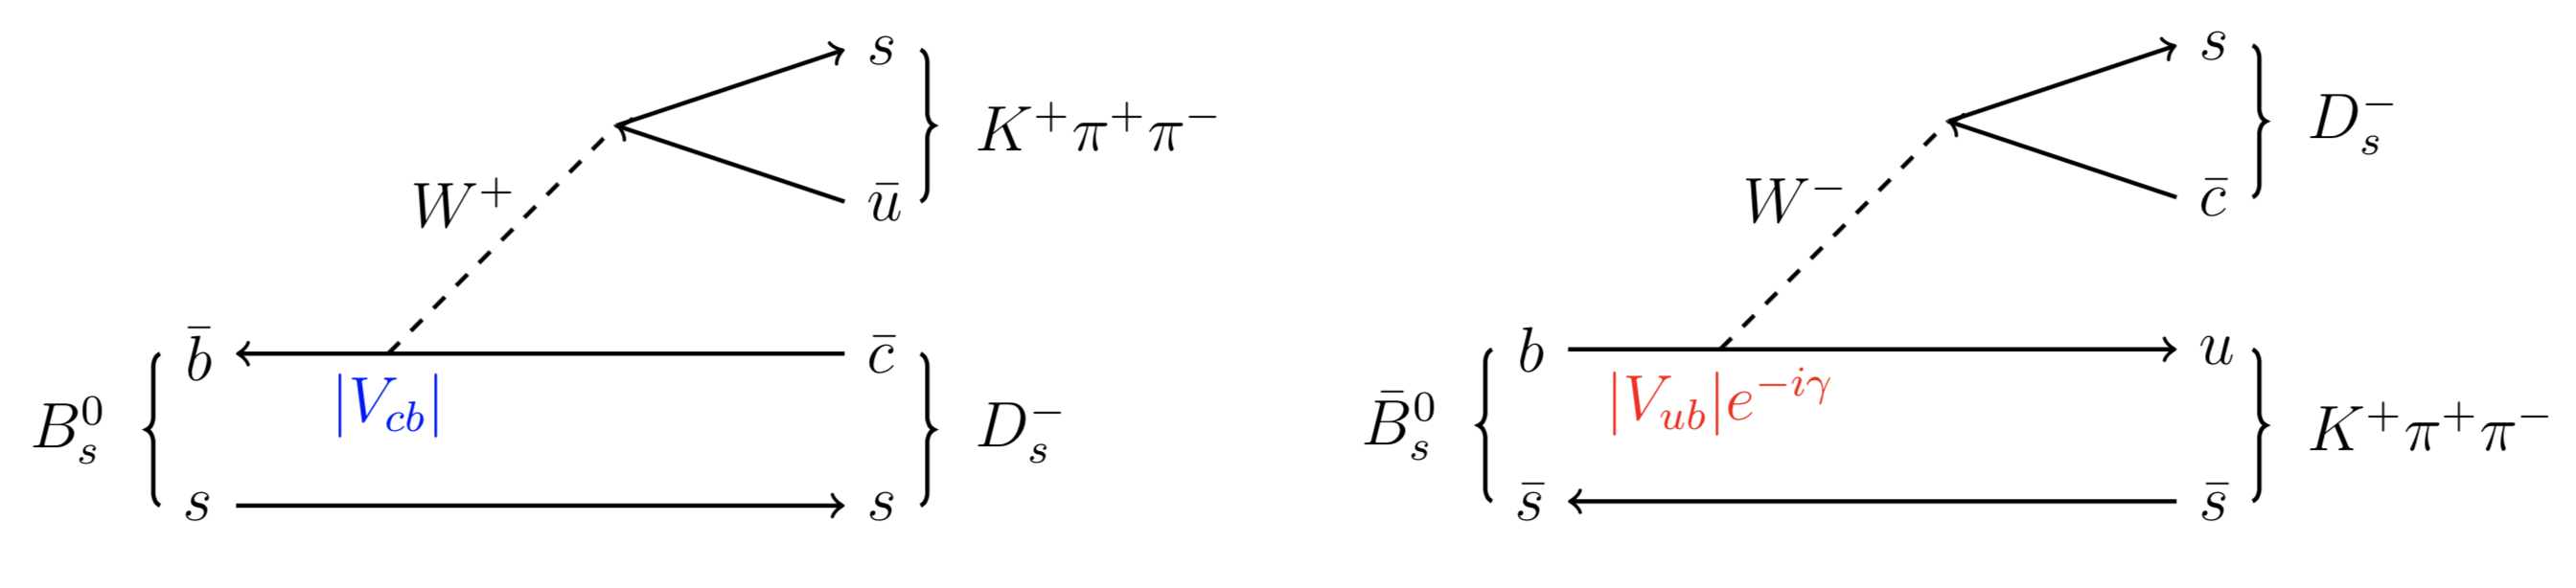
\includegraphics[height=!,width=\textwidth]{figs/feynman.png}
\caption{Feynman diagram for $B_s^0/\bar B_s^0 \to D_s^- K^+ \pip \pim$ decays.}
\label{fig:decay_feynman}
\end{figure}


%\begin{figure}[h]
%\centering
%%\tikzsetnextfilename{feynman_mixing.pdf}
%\begin{tikzpicture}[scale=1.]
%%Strange to beauty quark
%\draw [->,thick] (0,0) node[left]{$s$} -- (4,0) node[right]{$b$};
%%Beauty to strange Anti Quark
%\draw [<-,thick] (0,1) node[left]{$\bar{b}$} -- (4,1) node[right]{$\bar{s}$};
%%W boson
%\draw [dashed,thick] (2.5,0) -- (2.5,1);
%\draw [dashed,thick] (1.5,0) -- (1.5,1);
%
%%Labels
%\draw[decoration={brace},decorate,thick] (-0.5,0) -- node[left=0.2] {$B_s^0$} (-0.5,1);
%\draw[decoration={brace},decorate,thick] (4.5,1) -- node[right=6pt] {$\bar{B}_s^0$} (4.5,0);
%\node at (1.2,0.5) {$W$};
%\node at (2.8,0.5) {$W$};
%\node at (2,-0.3) {$u,c,t$};
%\node at (2,1.3) {$u,c,t$};
%\end{tikzpicture}
%\caption{Feynman diagram of $B_s$ mixing process.}
%\label{fig:mixing_feynman}
%\end{figure}
%
%
%\begin{figure}[h]
%\centering
%   
%\begin{subfigure}[b]{0.45\textwidth}
%
%\begin{tikzpicture}[scale=1]
%%Strange quark
%\draw [->,thick] (0,0) node[left]{$s$} -- (4,0) node[right]{$s$};
%%Beauty to Charm Quark
%\draw [<-,thick] (0,1) node[left]{$\bar{b}$} -- (4,1) node[right]{$\bar{c}$};
%\node at (1.,0.66) {$\textcolor{blue}{\vert V_{cb} \vert}$};
%
%%W+ boson
%\draw [dashed,thick] (1,1) -- (2.5,2.5);
%\node at (1.5,2) {$W^+$};
%%u Quark
%\draw [->,thick] (2.5,2.5) -- (4,3) node[right]{$s$};
%%d Quark
%\draw [<-,thick](2.5,2.5) -- (4,2) node[right]{$\bar{u}$};
%
%%pipipi brace and node
%\draw[decoration={brace},decorate,thick](4.5,3) -- node[right=6pt] {$K^+\pi^+\pi^-$} (4.5,2);
%%Ds brace and node
%\draw[decoration={brace},decorate,thick] (4.5,1) -- node[right=6pt] {$D_s^-$} (4.5,0);
%%Bs brace and node
%\draw[decoration={brace},decorate,thick] (-0.5,0) -- node[left=0.2] {$B_s^0$} (-0.5,1);
%\end{tikzpicture}
%
%\end{subfigure} \hfill
%%
%%
%%
%%
%%
%\begin{subfigure}[b]{0.45\textwidth}
%
%\begin{tikzpicture}[scale=1]
%%Strange quark
%\draw [<-,thick] (0,0) node[left]{$\bar s$} -- (4,0) node[right]{$\bar s$};
%%Beauty to Charm Quark
%\draw [->,thick] (0,1) node[left]{$b$} -- (4,1) node[right]{$u$};
%\node at (1.,0.66) {$\textcolor{red}{\vert V_{ub} \vert e^{-i\gamma}}$};
%%W+ boson
%\draw [dashed,thick] (1,1) -- (2.5,2.5);
%\node at (1.5,2) {$W^-$};
%%u Quark
%\draw [->,thick] (2.5,2.5) -- (4,3) node[right]{$s$};
%%d Quark
%\draw [<-,thick](2.5,2.5) -- (4,2) node[right]{$\bar{c}$};
%
%%pipipi brace and node
%\draw[decoration={brace},decorate,thick](4.5,3) -- node[right=6pt] {$D_s^-$} (4.5,2);
%%Ds brace and node
%\draw[decoration={brace},decorate,thick] (4.5,1) -- node[right=6pt] {$K^+\pi^+\pi^-$} (4.5,0);
%%Bs brace and node
%\draw[decoration={brace},decorate,thick] (-0.5,0) -- node[left=0.2] {$\bar B_s^0$} (-0.5,1);
%\end{tikzpicture}
%
%\end{subfigure}
%\caption{Feynman diagram for $B_s^0/\bar B_s^0 \to D_s^- K^+ \pip \pim$ decays.}
%\label{fig:decay_feynman}
%
%\end{figure}

\clearpage
% !TEX root = main.tex

\section{Sensitivity studies}


\subsection{PDF}

First, I define the purely hadronic amplitudes for a given phasespace point $x$.
The weak phase dependence is written latter explicitly in the pdf.

%\begin{align}
%	A(B_s^0 \to D_s^{-} K^{+} \pi\pi) &\equiv A(x) = \sum_i a_i \, A_i(x)   \\
%	A(\bar B_s^0 \to D_s^{-} K^{+} \pi\pi) &\equiv \bar A(x) = \sum_i \bar a_i \,\bar A_i(x)   \\
%	A(\bar B_s^0 \to D_s^{+} K^{-} \pi\pi) &= A(x)  \, \, \text{(Assuming no direct CPV)} \\
%	A(B_s^0 \to D_s^{+} K^{-} \pi\pi) &= \bar A(x)  \, \, \text{(Assuming no direct CPV)} 
%\end{align}

\begin{align}
	A(B_s^0 \to D_s^{-} K^{+} \pi\pi) &\equiv A(x) = \sum_i a_i \, A_i(x)   \\
	A(B_s^0 \to D_s^{+} K^{-} \pi\pi) &\equiv \bar A(\bar x) = \sum_i \bar a_i \,\bar A_i(\bar x)    \\
	A(\bar B_s^0 \to D_s^{-} K^{+} \pi\pi) &= \bar A(x)  \, \, \text{(Assuming no direct CPV)} \\
	A(\bar B_s^0 \to D_s^{+} K^{-} \pi\pi) &= A(\bar x)  \, \, \text{(Assuming no direct CPV)} 
\end{align}

The full time-dependent amplitude pdf is given by:
\begin{equation}
\begin{split}
\label{eq:PDF_full}
	P(x,t,q_t,q_f) &\propto  [
	 \left( \vert A(x) \vert^2 + \vert \bar A(x) \vert^2 \right) \, \text{cosh} \left( \frac{\Delta \Gamma \, t}{2}\right) \\
	 & + q_t q_f \left( \vert A(x) \vert^2 - \vert \bar A(x) \vert^2 \right) \, \text{cos} \left( m_s \, t \right)  \\
	 & -2 \text{Re}\left( A(x)^{*}  \bar A(x) \, e^{-i q_f (\gamma - 2\beta_s)}  \right) \, \text{sinh} \left( \frac{\Delta \Gamma \, t}{2}\right)  \\
	 & -2 q_t q_f \text{Im}\left( A(x)^{*}  \bar A(x) \, e^{-i q_f (\gamma - 2\beta_s)}  \right)\, \text{sin} \left( m_s \, t \right)  ]  e^{- \Gamma t}
\end{split}
\end{equation}
where $q_t = +1$ $(-1) $for a $B_s^{0}$ ($\bar B_s^{0}$) tag and 
$q_f$ = +1 $ $(-1) for $D_s^{-} K^{+} \pi\pi$ ($D_s^{+} K^{-} \pi\pi$) final states. \\

Integrating over the phasespace, we get
\begin{equation}
\begin{split}
\label{eq:PDF_intX}
	\int P(x,t,q_t,q_f) \text d x &\propto   [
	\, \text{cosh} \left( \frac{\Delta \Gamma \, t}{2}\right) \\
	 & + q_t q_f \left( \frac{1-r^2}{1+r^2} \right) \, \text{cos} \left( m_s \, t \right)  \\
	 & -2 \left( \frac{\kappa \, r \, \text{cos}(\delta - q_f(\gamma - 2 \beta_s))}{1+r^2}  \right) \, \text{sinh} \left( \frac{\Delta \Gamma \, t}{2}\right)  \\
	 & -2 q_t q_f \left( \frac{\kappa \, r \, \text{sin}(\delta - q_f(\gamma - 2 \beta_s))}{1+r^2}   \right)\, \text{sin} \left( m_s \, t \right)  ]  e^{- \Gamma t} \\
	 &=   [
	\, \text{cosh} \left( \frac{\Delta \Gamma \, t}{2}\right) 
	  + q_t q_f \, C \, \text{cos} \left( m_s \, t \right)  
	  - \textcolor{red}{\kappa} \, D_{q_f} \, \text{sinh} \left( \frac{\Delta \Gamma \, t}{2}\right)  
	  - q_t \, \textcolor{red}{\kappa} \, S_{q_f}\, \text{sin} \left( m_s \, t \right)  ]  e^{- \Gamma t}
\end{split}
\end{equation}
where the $C,D_{q_f},S_{q_f}$ are defined exactly as for $D_s K$.
The coherence factor is defined as :
\begin{align}
\label{eq:coherenceFactor}
	\kappa \, e^{i\delta} &\equiv \, \frac{\int A(x)^{*}  \bar A(x)  \text d x}{\sqrt{\int \vert A(x) \vert^2\text d x} \sqrt{\int \vert \bar A(x) \vert^2\text d x}  } \\
	r &\equiv \, \frac{\sqrt{\int \vert \bar A(x) \vert^2\text d x }}{\sqrt{\int \vert A(x) \vert^2\text d x}} 
\end{align}
and appears in front of the $D_{q_f},S_{q_f}$  terms.
This means one additional fit parameter for the lifetime fit.
In the limit of only one contributing resonance $\kappa \to 1$. \\


\subsection{Estimation of coherence factor}

To estimate the coherence factor we could generate many toys with random $a_i$ and $\bar a_i$ values (see https://twiki.cern.ch/twiki/pub/LHCbPhysics/Bu2DKstar/LHCb-ANA-2017-005\_v1.pdf) using the set of amplitudes show in our last talk. However with so many interfering amplitudes, I would be surprised if you couldn't generate every possible value for $\kappa$. In any case, this would give us a  range where to expect possible values for $\kappa$. Worst case would be $0 \leq \kappa \leq 1$. \\

Assumptions:
	\begin{itemize}
		\item   $A(x) = \sum_i a_i \, A_i(x)$   \\
		 $\bar A(x) = \sum_i \bar a_i \, \bar A_i(x)$
		\item Use amplitudes from flavor-averaged, time-integrated fit
		 \item Draw random $a_i$ and $\bar a_i $ values
		 \item Constraints: \\
		 $\int ( \vert a_i  A_i(x) \vert^2 + \vert \bar a_i  \bar A_i(x) \vert^2 ) \, \text{d}x / N = F^{eff}_i $ \\
		 $r \approx 0.4 $ (ration of CKM elements)
	\end{itemize}
	
\begin{figure}[hp]
	\centering
		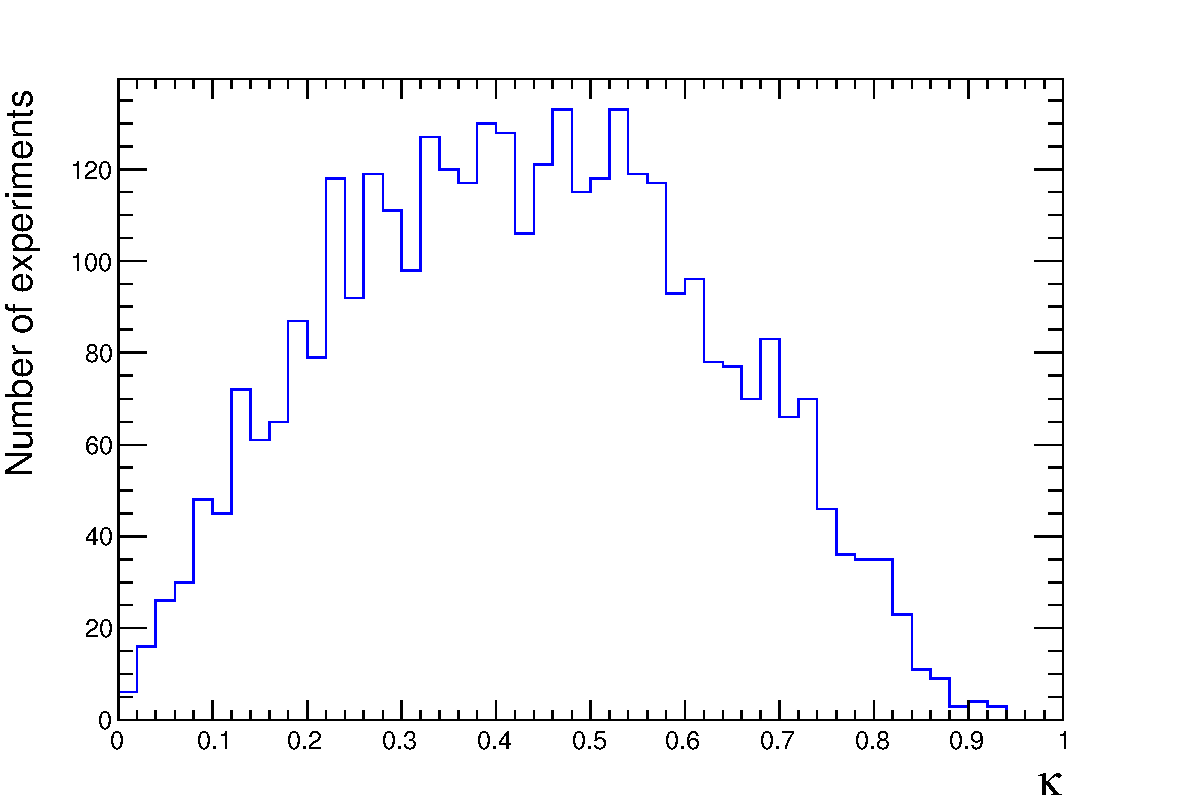
\includegraphics[width=0.35\textwidth, height = 3.cm]{figs/plots/k-eps-converted-to.pdf} 
		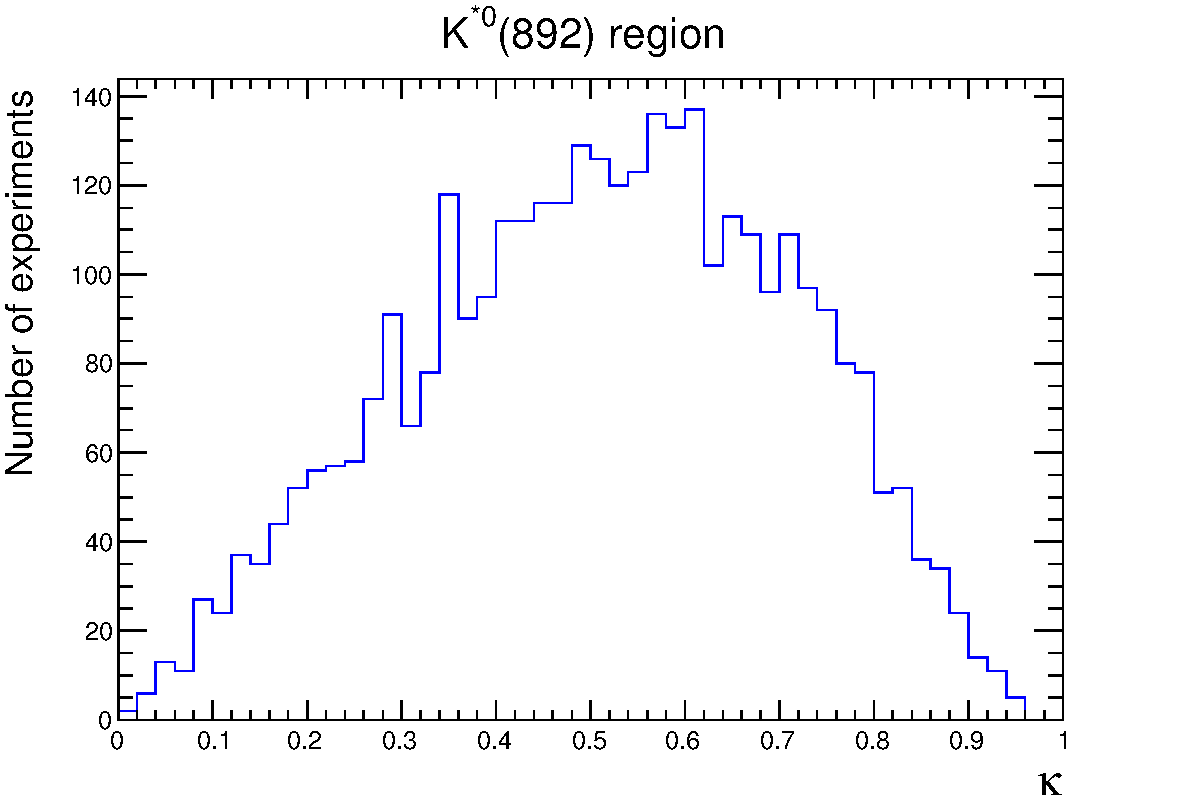
\includegraphics[width=0.35\textwidth, height = 3.cm]{figs/plots/k_Ks-eps-converted-to.pdf} 
		
		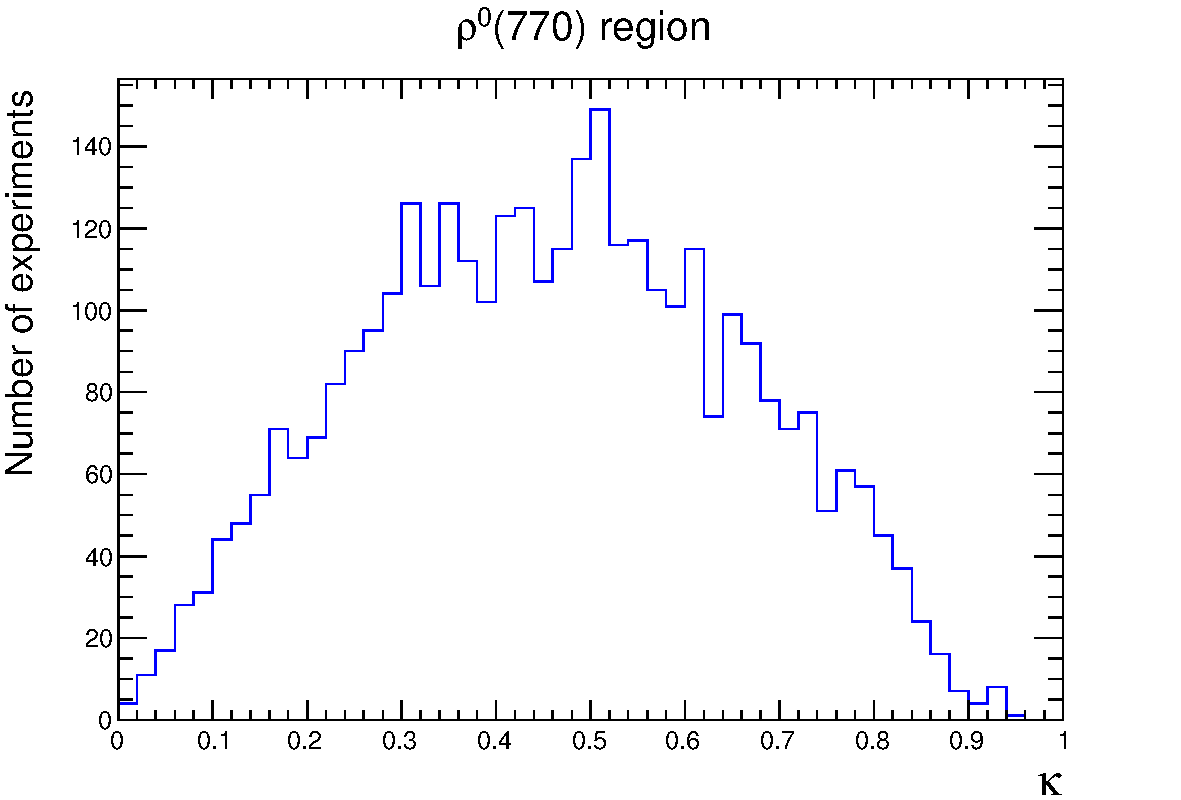
\includegraphics[width=0.35\textwidth, height = 3.cm]{figs/plots/k_rho-eps-converted-to.pdf} 
		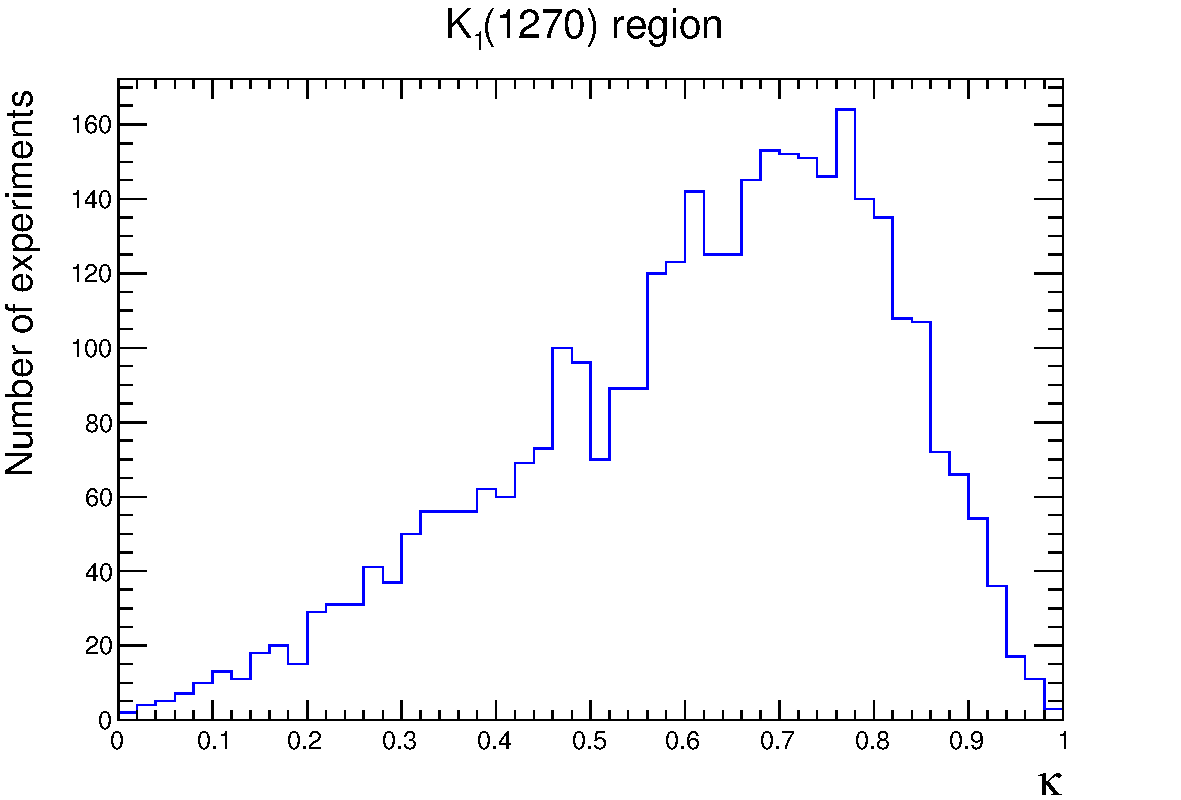
\includegraphics[width=0.35\textwidth, height = 3.cm]{figs/plots/k_K1-eps-converted-to.pdf} 	
		\caption{}	
\end{figure}		

	\begin{table}[h]
			\caption{}	
  \footnotesize
  \centering
  \begin{tabular}
    {l c c }
    \hline \hline
    Region &  $<\kappa> (\%)$   &  Cut eff. $(\%)$ \\   \hline
    Full & 43 &  100 \\
    $K^*(892)$ & 51    &  43  \\
    $\rho^0(770)$ & 46  & 47   \\
    $K_1(1270)$ & 61   & 23  \\
    \hline \hline
  \end{tabular}
  \label{tab:sideband}
\end{table}


%The next option would be to fit the flavor tagged Dalitz plot which would allow us to really predict $\kappa$ (together with $r$ and $\delta$ actually). 
%Integrating the full pdf over  time, we get
%\begin{align*}
%	\int P(x,t,q_t,q_f) \text d t &\propto   
%	 \left( \vert A(x) \vert^2 + \vert \bar A(x) \vert^2 \right) \, \frac{4\Gamma}{4\Gamma^2-\Delta \Gamma^2} \\
%	 & + q_t q_f \left( \vert A(x) \vert^2 - \vert \bar A(x) \vert^2 \right) \, \frac{\Gamma}{\Gamma^2+m_s^2} \\
%	 & -2 \text{Re}\left( A(x)^{*}  \bar A(x) \, e^{-i q_f (\gamma - 2\beta_s)}  \right) \,\frac{2\Delta\Gamma}{4\Gamma^2-\Delta \Gamma^2} \\
%	 & -2 q_t q_f \text{Im}\left( A(x)^{*}  \bar A(x) \, e^{-i q_f (\gamma - 2\beta_s)}  \right)\, \frac{m_s}{\Gamma^2+m_s^2} 
%\end{align*}
%
%I think that is a very interesting result since it shows that we could in principle also measure $\gamma$ with a time-independent 
%amplitude fit. But no idea how sensitive this would be. Probably not so much since the prefactors of the third and forth term are at least one order of 
%magnitude smaller than the first term.
%Unfortunately, the sensitivity to the coherence factor also comes mainly from the third and forth term. \\
%If we just want to estimate $\kappa$ from this fit and then use it for the lifetime fit, the potential $\gamma$ sensitivity of the Dalitz fit is another problem. 
%We could fix $\gamma$ to the world average for the dalitz fit but this might introduce some bias.
%Better would be to average over the final state flavor in which case the sensitivity to gamma would be lost. \\
%
%In summary, I think it is very hard to disentangle $A(x)$ and $\bar A(x)$ from a time integrated fit since the oscillation frequency is so large.
%We might be able to get some estimate but in the end, the lifetime fit has to determine the precise value.
%A full time dependent amplitude fit would of course be the most sensitive approach (but model-dependent).

\clearpage
\subsection{Results}

Assumptions:
	\begin{itemize}	
		\item Use amplitudes from flavor-averaged, time-integrated fit
		\item $r = 0.4$ (ratio of CKM elements) 
		\item PDG values for: $\tau,\Delta m_s, \Delta \Gamma, \beta_s$
		\item $\epsilon(x,t) = const.$, perfect resolution  
		\item $\epsilon_{Tag} = 0.66, <\omega> = 0.4 $   
		\item $N_{signal} = 3000$ (Run1+15/16 data)		 
	\end{itemize}
	
	
		\begin{figure}[hp]
	\centering
		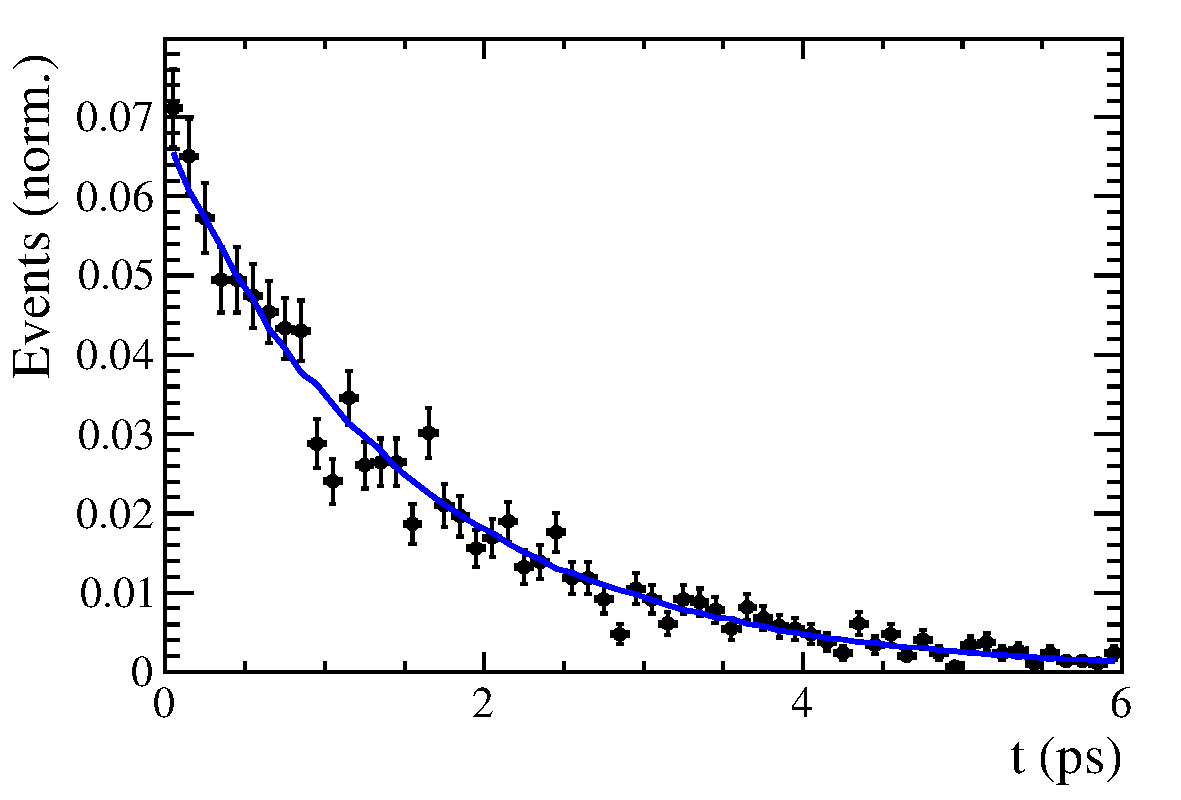
\includegraphics[width=0.45\textwidth, height = !]{figs/plots_toy/h_t-eps-converted-to.pdf} 
		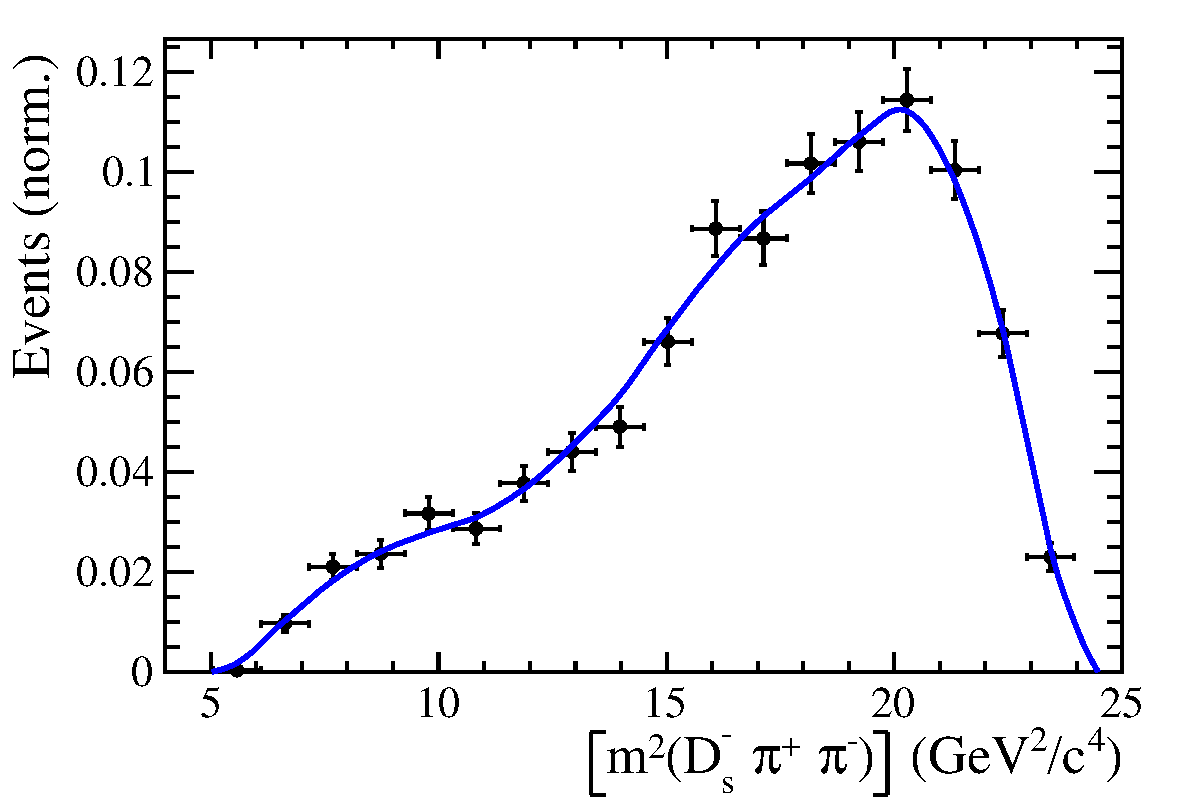
\includegraphics[width=0.45\textwidth, height = !]{figs/plots_toy/s_Dspipi-eps-converted-to.pdf} 
		
		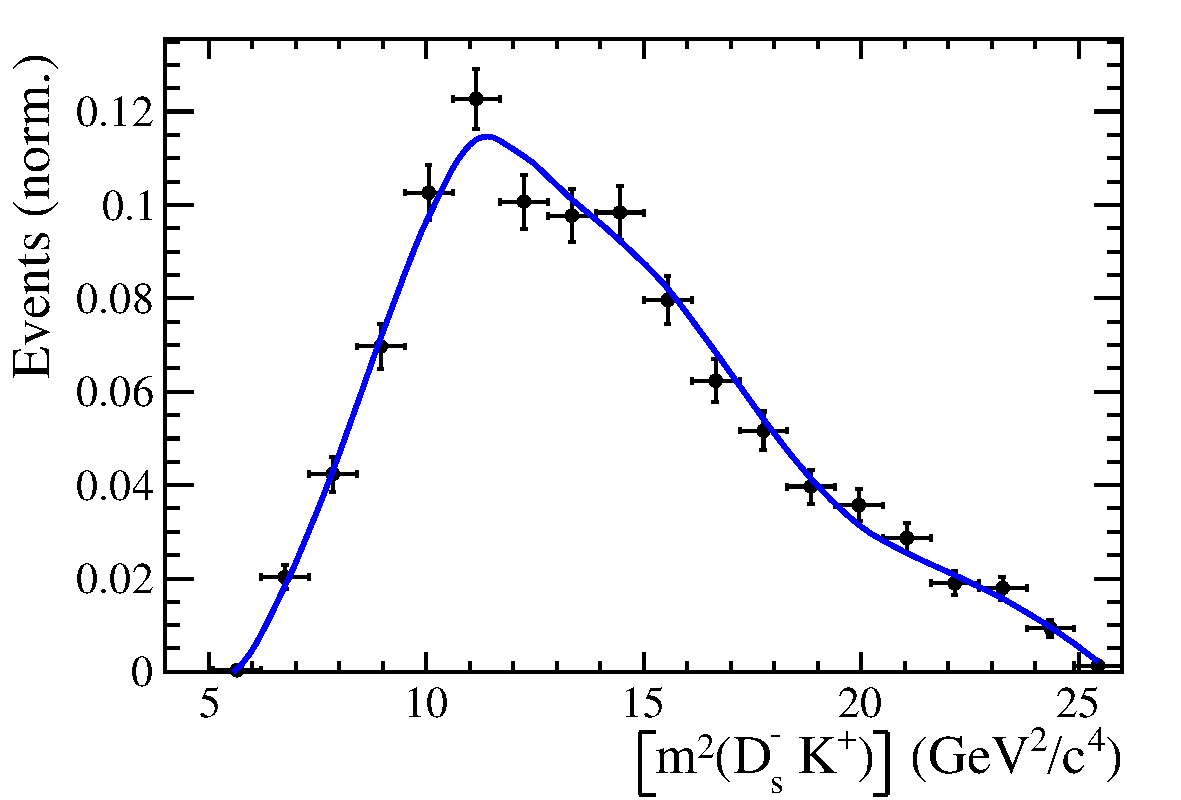
\includegraphics[width=0.45\textwidth, height = !]{figs/plots_toy/s_DsK-eps-converted-to.pdf} 
		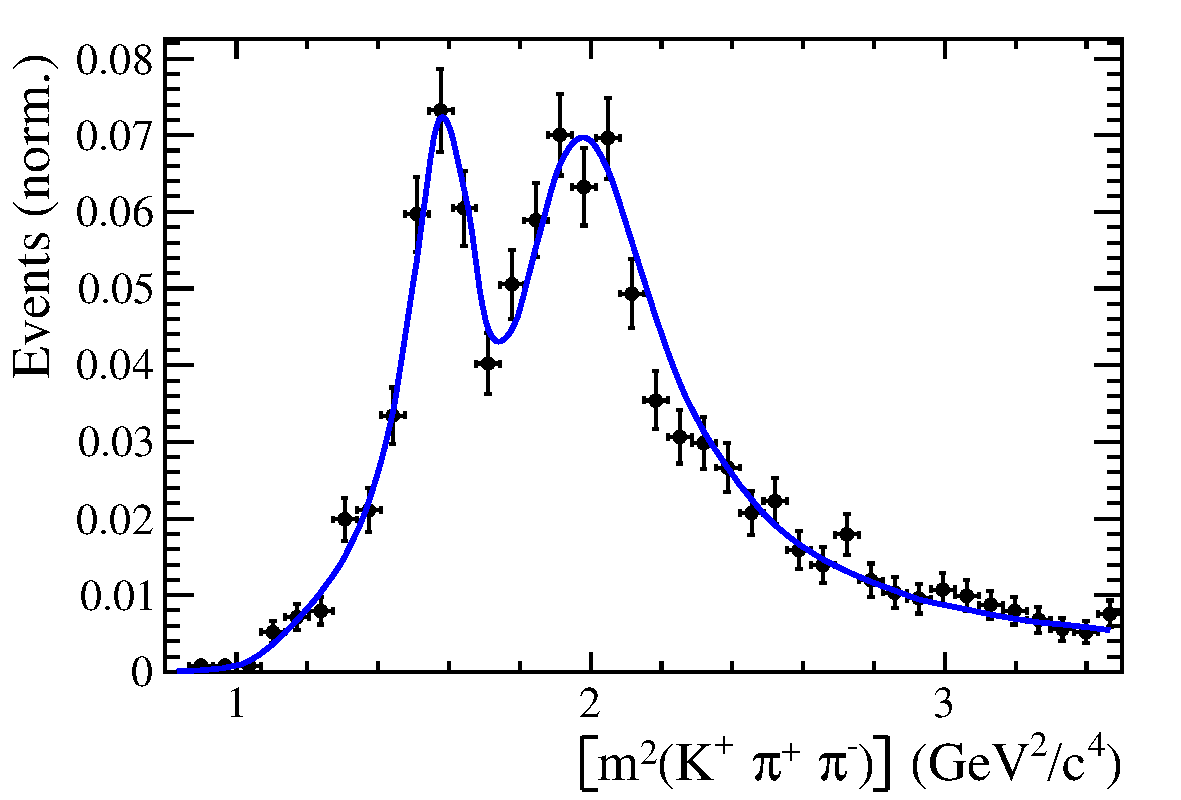
\includegraphics[width=0.45\textwidth, height = !]{figs/plots_toy/s_Kpipi-eps-converted-to.pdf}
		 
		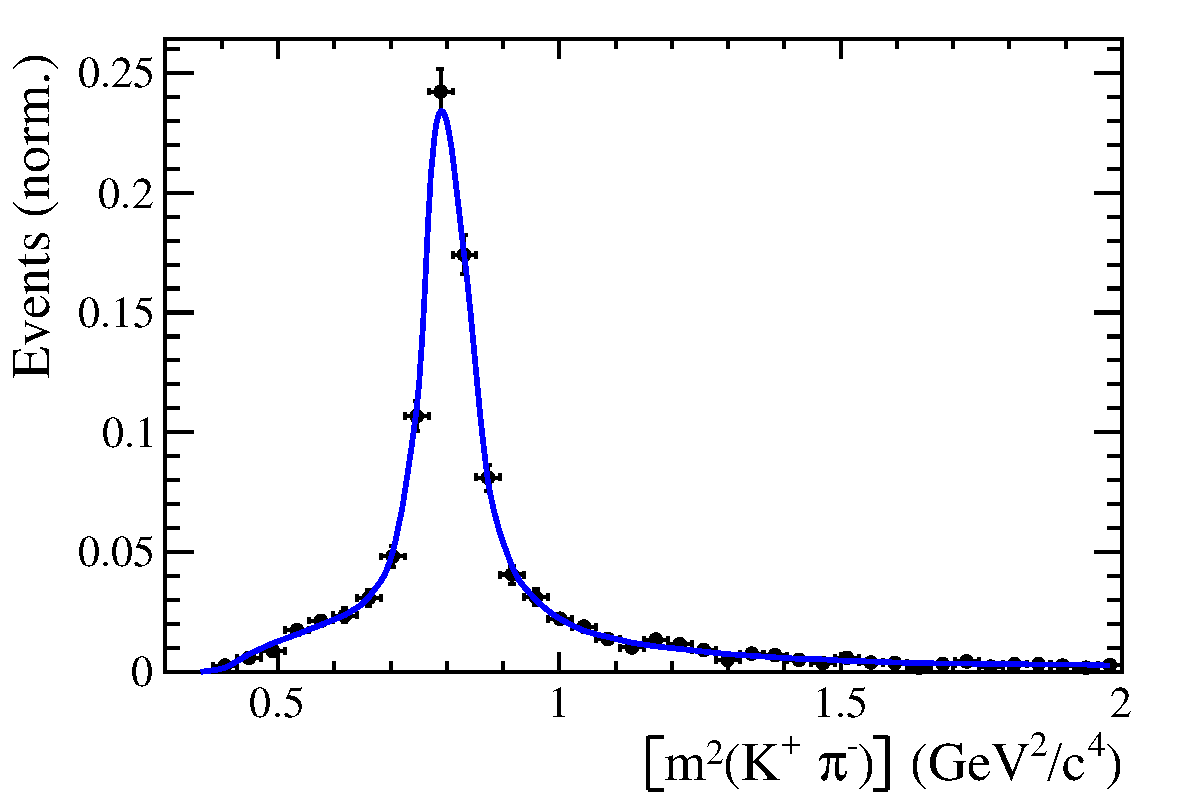
\includegraphics[width=0.45\textwidth, height = !]{figs/plots_toy/s_Kpi-eps-converted-to.pdf} 
		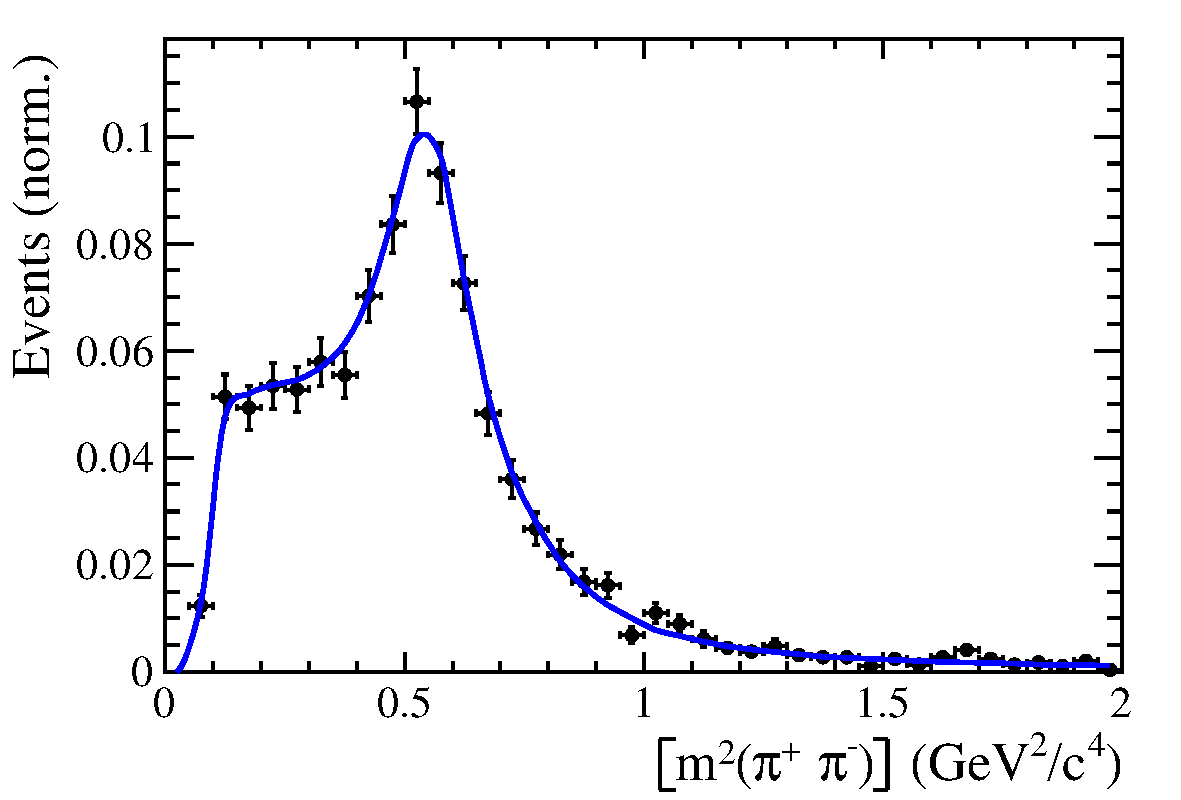
\includegraphics[width=0.45\textwidth, height = !]{figs/plots_toy/s_pipi-eps-converted-to.pdf}
		
		\caption{Example toy fit} 		
	\end{figure}				


	\begin{figure}[hp]
	\centering
		
%		$D_s^+ K^- \pi \pi$      \hspace{2cm}     $D_s^- K^+ \pi \pi$   \hspace{2cm}   Combined
%		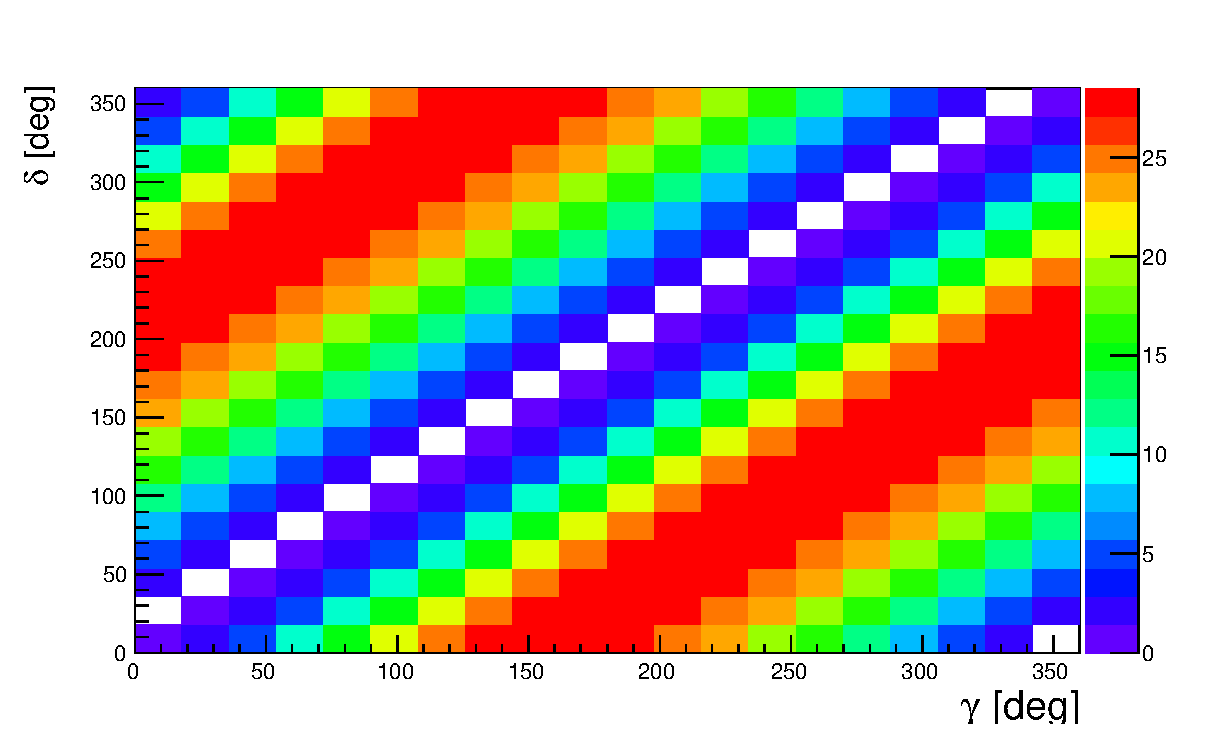
\includegraphics[width=0.4\textwidth, height = 4 cm{plots/LL_scan_m.eps} 
%		\includegraphics[width=0.4\textwidth, height = 4 cm]{plots/LL_scan_p.eps} 
		
		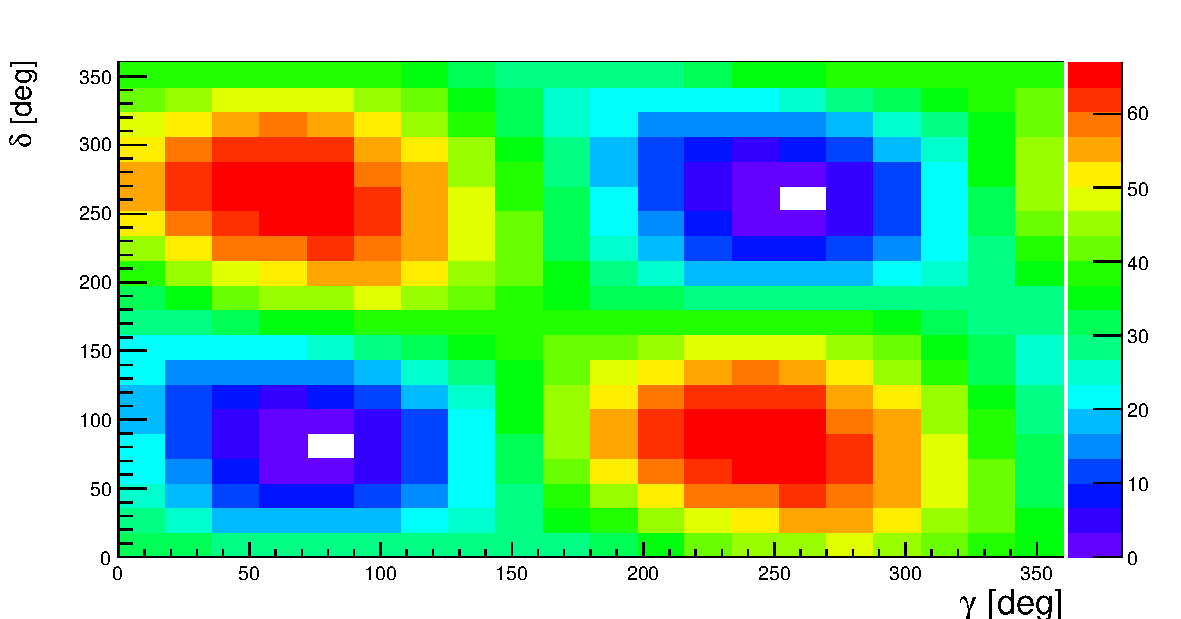
\includegraphics[width=0.45\textwidth, height = 4 cm]{plots/LL_scan-eps-converted-to.pdf} 
		
		Generated values: \\  $\gamma = 70^{\circ}, \delta = 100^{\circ}$ \\
		Fit result:    \\ $\gamma = 74 \pm 15^{\circ}, \delta = 84 \pm 15^{\circ}$ \\
		 ($\gamma = 254 \pm 15^{\circ}, \delta = 264 \pm 15^{\circ}$)

		\caption{Likelihood scan} 		

	\end{figure}	


	\begin{figure}[hp]
	\centering
		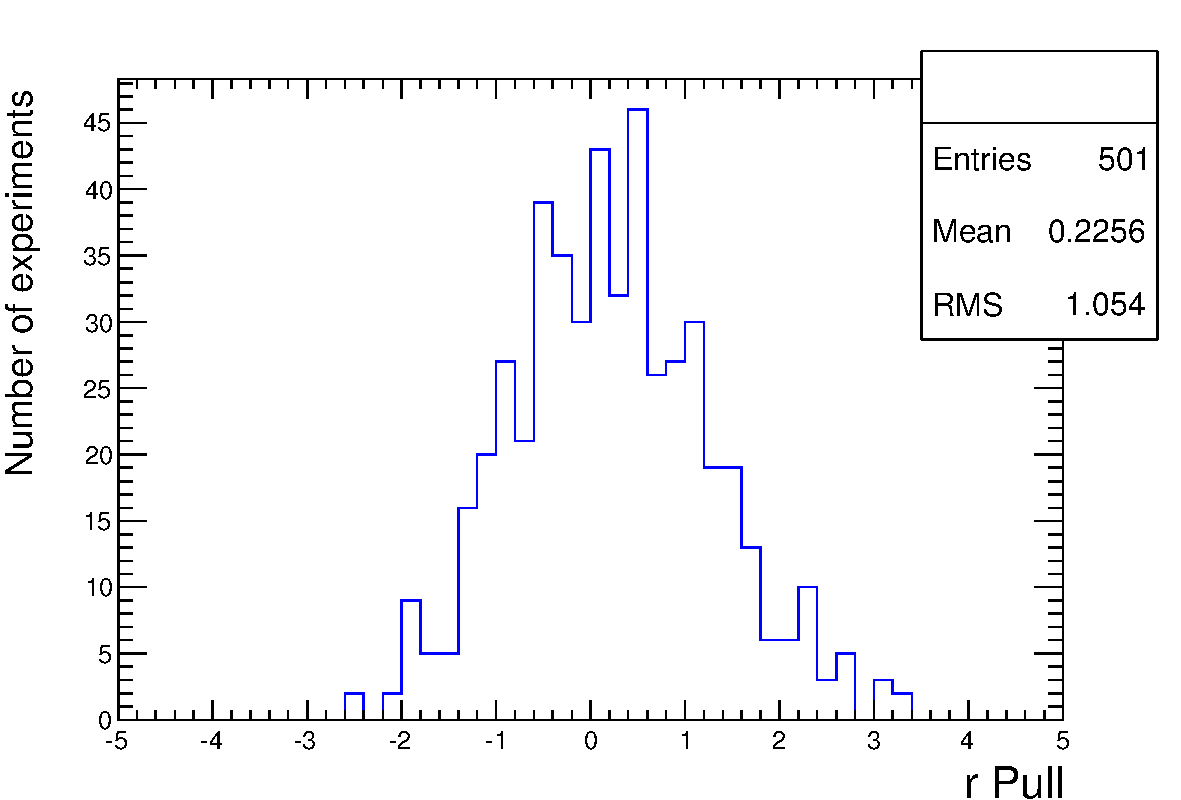
\includegraphics[width=0.4\textwidth, height = 3.cm]{figs/plots_toy/r_pull-eps-converted-to.pdf} 
		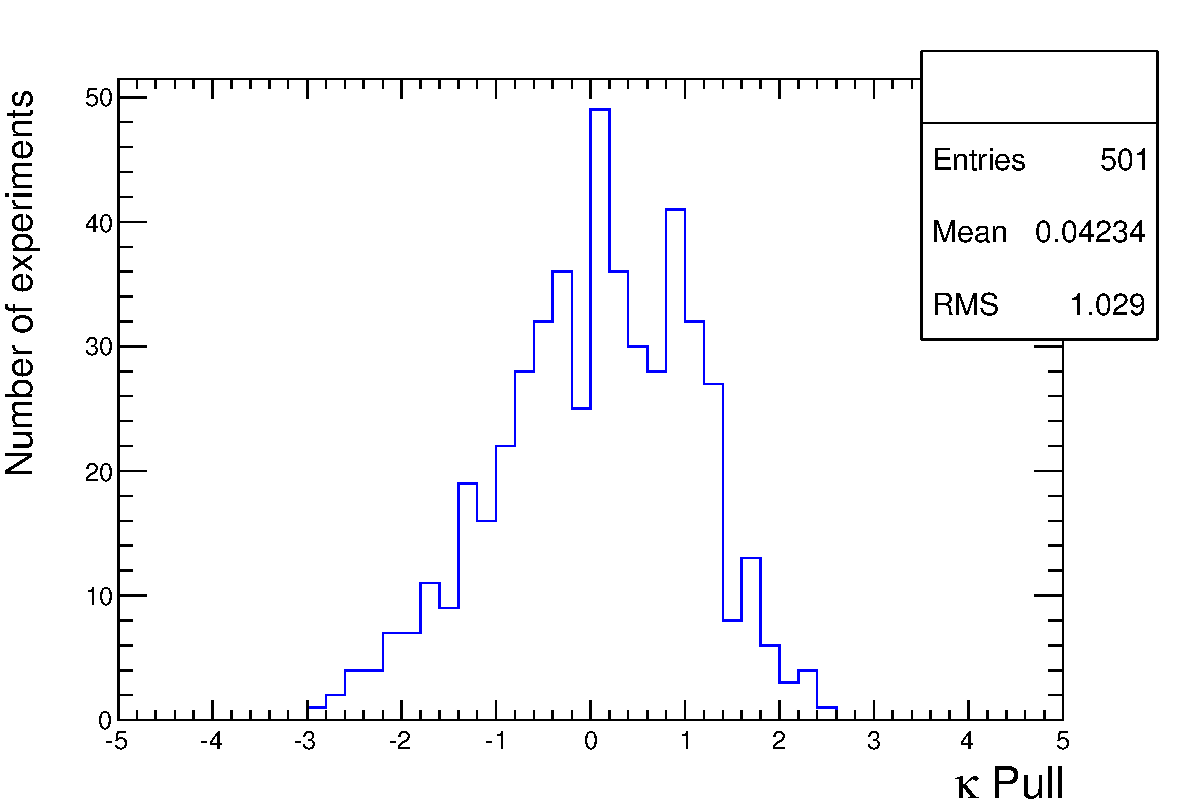
\includegraphics[width=0.4\textwidth, height = 3.cm]{figs/plots_toy/k_pull-eps-converted-to.pdf} 
		
		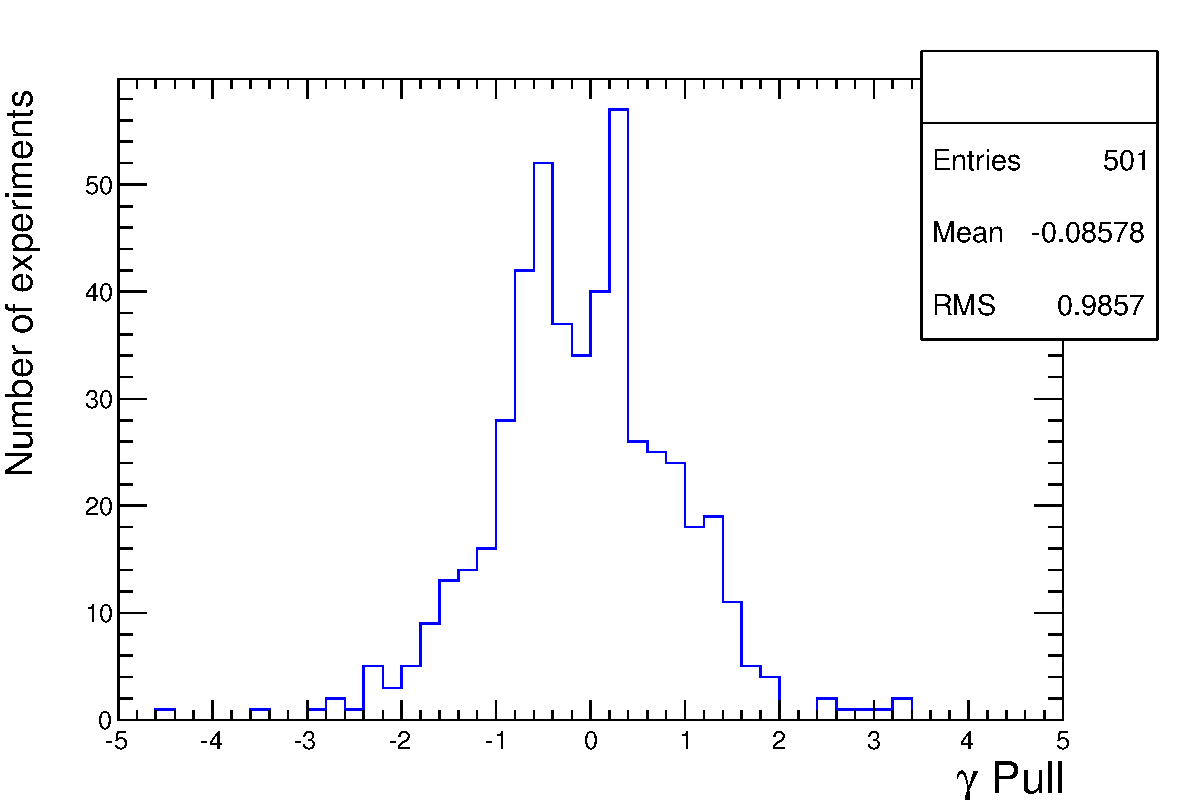
\includegraphics[width=0.4\textwidth, height = 3.cm]{figs/plots_toy/gamma_pull-eps-converted-to.pdf} 
		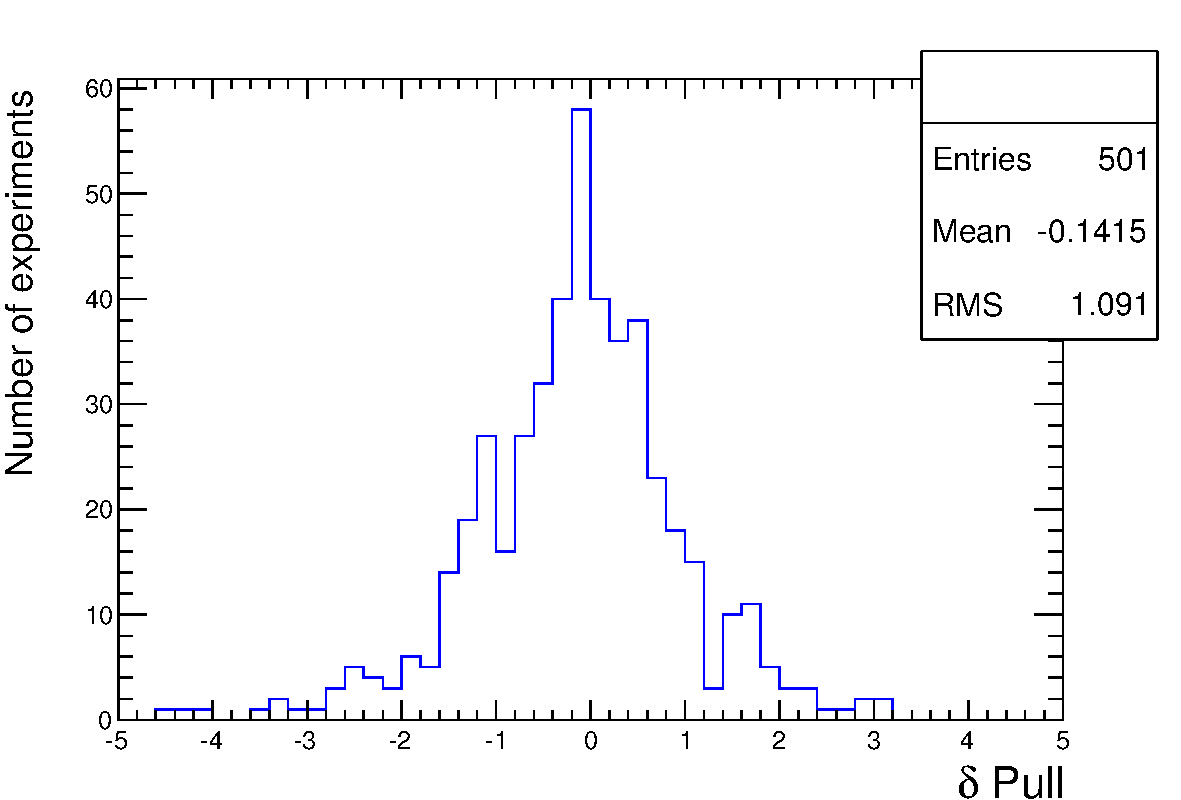
\includegraphics[width=0.4\textwidth, height = 3.cm]{figs/plots_toy/delta_pull-eps-converted-to.pdf} 

		\caption{Pulls} 		

	\end{figure}	
	

\clearpage	

\begin{table}[h]
	\caption{} 		
  \scriptsize
  \centering
  \begin{tabular}
    {l c c c c}
    \hline \hline
    & Generated &  Full PDF     &   Phasespace integrated  \\   \hline
	$r$ & 0.4 & $0.38 \pm 0.06$   &  unstable \\
	$\kappa$  & \textcolor{red}{0.2} & $0.23 \pm 0.13$ & 0.2 (fixed)  \\
	$\delta$ & 100 & $99 \pm 22$ &  unstable\\
	$\gamma$ & 70 & $70 \pm 17$  & unstable \\
    \hline \hline
  \end{tabular}

  \begin{tabular}
    {l c c c c}
    \hline \hline
    & Generated &  Full PDF    &   Phasespace integrated  \\   \hline
	$r$ & 0.4 & $0.44 \pm 0.07$      & $0.43 \pm 0.11$  \\
	$\kappa$  & \textcolor{red}{0.4} &$0.41 \pm 0.14$  & 0.4 (fixed)  \\
	$\delta$ & 100 & $101 \pm 19$  & $95 \pm 41$ \\
	$\gamma$ & 70 & $69 \pm 16$   & $66 \pm 40 $ \\
    \hline \hline
  \end{tabular}

  \begin{tabular}
    {l c c c c}
    \hline \hline
    & Generated &  Full PDF    &   Phasespace integrated  \\   \hline
	$r$ & 0.4 & $0.41 \pm 0.08$     & $0.39 \pm 0.11$  \\
	$\kappa$  & \textcolor{red}{0.6} & $0.60 \pm 0.13$  & 0.6 (fixed)  \\
	$\delta$ & 100 & $98 \pm 17$ & $92 \pm 25$ \\
	$\gamma$ & 70 & $68 \pm 17$ & $65 \pm 28$ \\
    \hline \hline
  \end{tabular}

  \begin{tabular}
    {l c c c c}
    \hline \hline
    & Generated &  Full PDF        &   Phasespace integrated  \\   \hline
	$r$ & 0.4 & $0.42 \pm 0.09$    &  $0.39 \pm 0.09$ \\
	$\kappa$  & \textcolor{red}{1.0} & $0.96 \pm 0.03$ &  1.0 (fixed)  \\
	$\delta$ & 100 & $100 \pm 17$ &  $100 \pm 17$  \\
	$\gamma$ & 70 & $66 \pm 17$ & $67 \pm 17$  \\
    \hline \hline
  \end{tabular}
\end{table}


\clearpage
\section{Selection}
\label{sec:Selection}

For the presented analysis, we reconstruct the $\Bs\to\Ds\kaon\pion\pion$ decay through three different final states of the $\Ds$ meson, $\Ds\to\kaon\kaon\pion$, $\Ds\to\kaon\pion\pion$ and $\Ds\to\pion\pion\pion$.
Of those three final states $\Ds\to\kaon\kaon\pion$ is the most prominent one,
 while $\mathcal{BR}(\Ds\to\pion\pion\pion) \approx 0.2\cdot\mathcal{BR}(\Ds\to\kaon\kaon\pion)$ and $\mathcal{BR}(\Ds\to\kaon\pion\pion) \approx 0.1\cdot\mathcal{BR}(\Ds\to\kaon\kaon\pion)$ holds for the other two. \newline
A two-fold approach is used to isolate the $\Bs\to\Ds\kaon\pion\pion$ candidates from data passing the stripping line. 
First, further one-dimensional cuts are applied to reduce the level of combinatorial background and to veto some specific physical background. 
This stage is specific to the respective final state in which the $\Ds$ meson is reconstructed, since different physical backgrounds, depending on the respective final state, have to be taken into account.   
After that, a multivariate classifier is trained which combines the information of several input variables, including their correlation, into one powerful discriminator
between signal and combinatorial background. For this stage, all possible $\Ds$ final states are treated equally. 

\subsection{Cut-based selection}

In order to minimize the contribution of combinatorial background to our samples, we apply the following cuts to the b hadron:

\begin{itemize}

\item DIRA $>$ 0.99994

\item min IP $\chi^{2}$ $<$ 20 to any PV,

\item FD $\chi^{2}$ $>$ 100 to any PV,

\item Vertex $\chi^{2}$/nDoF $<$ 8,

\item ($Z_{\Ds}-Z_{\Bs}$) $>$ 0 , where $Z_{M}$ is the z-component of the position $\vec{x}$ of the decay vertex for the $\Bs$/$\Ds$ meson.

\end{itemize}    


Additionally, we veto various physical backgrounds, which have either the same final state as our signal decay, or can contribute via a single misidentification of $\kaon\to\pion$ or $\kaon\to\proton$. 
In the following, the vetoes are ordered by the reconstructed $\Ds$ final state they apply to: 


\begin{enumerate}

\item All:

\begin{enumerate}

\item $\Bs\to\Dsp\Dsm$ : $|M(\kaon\pion\pion) - m_{\Ds}| >$ 20 $\mevcc$.

\item $\Bs\to\Ds^{-}\Kp\Km\pip$ : possible with single missID of $\Km\rightarrow\pim$, rejected by requiring $\pim$ to fulfill $\dllkpi$ $<$ 5. 

\end{enumerate}

\item $\Ds\to\kaon\kaon\pion$

\begin{enumerate}

\item $\Bz\to\Dp(\to\Kp\pim\pip)\kaon\pion\pion$ : possible with single missID of $\pip\rightarrow\Kp$, vetoed by changing particle hypothesis and recompute $|M(\Kp\pim\pip) - m_{Dp}|$ $>$ 30 $\mevcc$, 
or the $\Kp$ has to fulfill $\dllkpi$ $>$ 10.

\item $\Lb\to\Lc(\to\proton\Km\pip)\kaon\pion\pion$ : possible with single missID of $\proton\rightarrow\Kp$, vetoed by changing particle hypothesis and recompute $M(\proton\Km\pip) - m_{\Lc}$ $>$ 30 $\mevcc$, 
or the $\Kp$ has to fulfill ($\dllkpi$ - $\dllppi$) $>$ 5.

\item $\Dz\to\kaon\kaon$ : $\Dz$ combined with a random $\pion$ can fake a $\Ds\to\kaon\kaon\pion$ decay and be a background to our signal, vetoed by requiring $M(\kaon\kaon) < 1840 \mevcc$. 

\end{enumerate}

\item $\Ds\to\kaon\pion\pion$

\begin{enumerate}

\item $\Dz\to\pip\Km$ : $\Dz$ combined with a random $\pim$ can fake a $\Ds^{-}\to\Km\pip\pim$ decay and be a background to our signal, vetoed by requiring $M(\pip\Km) < 1750 \mevcc$.

\item $\Lb\to\Lc(\to\proton\pim\pip)\kaon\pion\pion$ : possible with single missID of $\proton\rightarrow\Kp$, vetoed by changing particle hypothesis and recompute $M(\proton\pim\pip) - m_{\Lc}$ $>$ 30 $\mevcc$, 
or the $\Kp$ has to fulfill ($\dllkpi$ - $\dllppi$) $>$ 5.

\end{enumerate}

\item $\Ds\to\pion\pion\pion$

\begin{enumerate}

\item $\Dz\to\pion\pion$ : combined with a random $\pion$ can fake a $\Ds\to\pion\pion\pion$ decay and be a background to our signal, vetoed by requiring both possible combinations to have $M(\pion\pion) < 1700 \mevcc$.

\end{enumerate}

\end{enumerate}


The most prominent final state used in this analysis is $\Bs\to\Ds(\to\kaon\kaon\pion)\kaon\pion\pion$, 
where the $\Ds$ decay can either proceed via the narrow $\phiz$ resonance, the broader $\Kstarz$ resonance, or non resonant.
Depending on the decay process being resonant or not, we apply additional PID requirements on this final state:

\begin{itemize}

\item resonant case: 
\begin{itemize}
\item $\Dsp\to\phiz\pip$, with $|M(\Kp\Km) - m_{\phiz}|$ $<$ 20 $\mevcc$ : no additional requirements, since $\phiz$ is narrow and almost pure $\Kp\Km$. 
\item $\Dsp\to\Kstarzb\Kp$, with  $|M(\Km\pip) -m_{\Kstarz}|$ $<$ 75 $\mevcc$ :  $\dllkpi$ $>$ 0 for kaons, since this resonance is more than ten times broader than $\phiz$. 
\end{itemize}

\item non resonant case: $\dllkpi$ $>$ 5 for kaons, since the non resonant category has significant charmless contributions.

\end{itemize}



For the other two final states, we apply global PID requirements:



\begin{itemize}

\item  $\Ds\to\kaon\pion\pion$

\begin{itemize}

\item  $\dllkpi$ $>$ 10 for kaons, since we expect significantly higher charmless background contribution in this channel. 

\item  $\dllkpi$ $<$ 5 for pions.

\end{itemize}

\item $\Ds\to\pion\pion\pion$

\begin{itemize}

\item $\dllkpi$ $<$ 10 for all pions.

\item $\dllppi$ $<$ 10 for all pions.

\end{itemize}

\end{itemize}


%Since a measurement of the weak CKM phase $\gamma$ in the $\Bs\to\Ds\kaon\pion\pion$ channel will almost certainly be statistically limited, 
%we plan to add also the $\Ds\to\pion\pion\pion$ final state with $\mathcal{BR}(\Ds\to\pion\pion\pion) \approx 0.2\cdot\mathcal{BR}(\Ds\to\kaon\kaon\pion)$ to the $\gamma$ analysis. 
%Since the determination of the branching ratio is expected to have the same level of statistical and systematical uncertainties and due to the additional complexity (different selection, efficiencies, simulated samples), 
%we choose to only use the most prominent $\Ds\to\kaon\kaon\pion$ final state for the BR determination. 


\subsection{Multivariate stage}

We use TMVA \cite{Hocker:2007ht} to train a multivariate discriminator, which is used to further improve the signal to background ratio. 
The 17 variables used for the training are:

\begin{itemize} 

\item max(ghostProb) over all tracks

\item cone($\pt$) asymmetry of every track, 
which is defined to be the difference between the $\pt$ of the $\pi$/$\kaon$ and the sum of all other $\pt$ in a cone of radius $r = \sqrt{(\Delta\Phi)^{2} + (\Delta\eta)^{2}}$ $<$ 1 rad around the signal $\pi$/$\kaon$ track.

\item min(IP$\chi^{2}$) over the $X_{s}$ daughters

\item max(DOCA) over all pairs of $X_{s}$ daughters

\item min(IP$\chi^{2}$) over the $\Ds$ daughters

\item $\Ds$ and $\Bs$ DIRA

\item $\Ds$ FD significance

\item max($\cos(\Ds h_{i})$), where $\cos(\Ds h_{i})$ is the cosine of the angle between the $\Ds$ and another track i in the plane transverse to the beam

\item $\Bs$ IP$\chi^{2}$, FD$\chi^{2}$ and Vertex $\chi^{2}$

\end{itemize}

Various classifiers were investigated in order to select the best performing discriminator. Consequently, a boosted decision tree with gradient boost (BDTG) is chosen as nominal classifier. 
We use truth-matched MC as signal input. 
Simulated signal candidates are required to pass the same trigger, stripping and preselection requirements, that were used to select the data samples.  
For the background we use events from the high mass sideband ($m_{\Bs candidate}$ $>$ 5600 $\mevcc$) of our data samples. 
As shown in Fig. \ref{fig:massforBDT}, this mass region is sufficiently far away from signal structures and is expected to be dominantly composed of combinatorial background. \newline

\begin{figure}[h]
%\vspace*{-0.4cm}
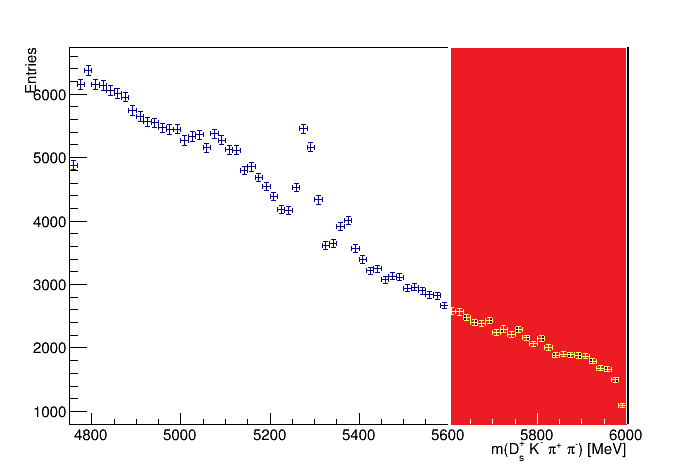
\includegraphics[height=7.4cm,width=0.7\textwidth]{figs/mass_Bs_forBDT_12_AnA.png}
%\vspace*{-0.2cm}
\caption{Invariant mass distribution of preselected $\Bs\to\Ds\kaon\pion\pion$ candidates. The red coloured region with $m_{\Bs candidate}$ $>$ 5600 $\mevcc$ is used as background input for the boosted decision tree.}
\label{fig:massforBDT}
\end{figure}

The distributions of the input variables for signal and background are shown in Fig. \ref{fig:BDT_Input_1}. 

\begin{figure}[h]
%\vspace*{-0.4cm}
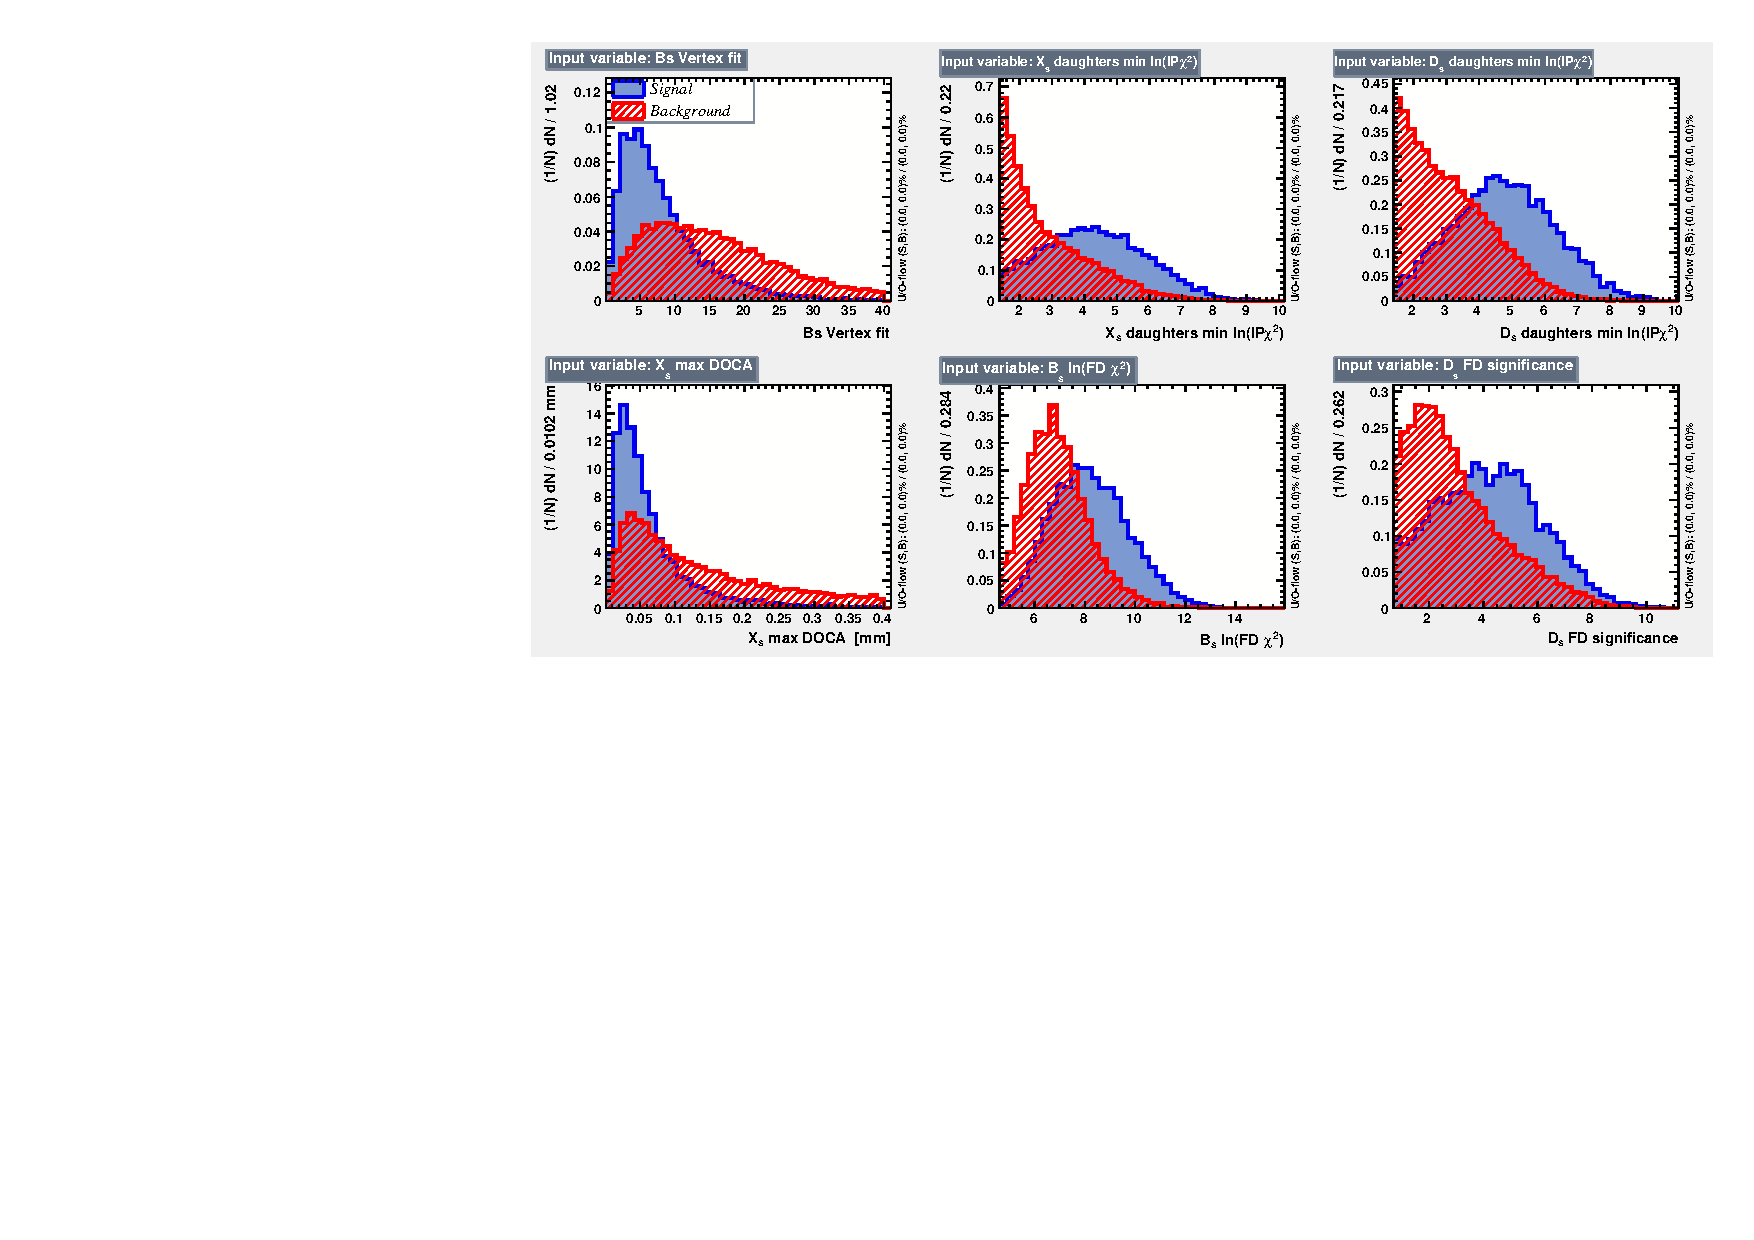
\includegraphics[height=6.cm,width=0.95\textwidth]{figs/BDT_Input_1.pdf}
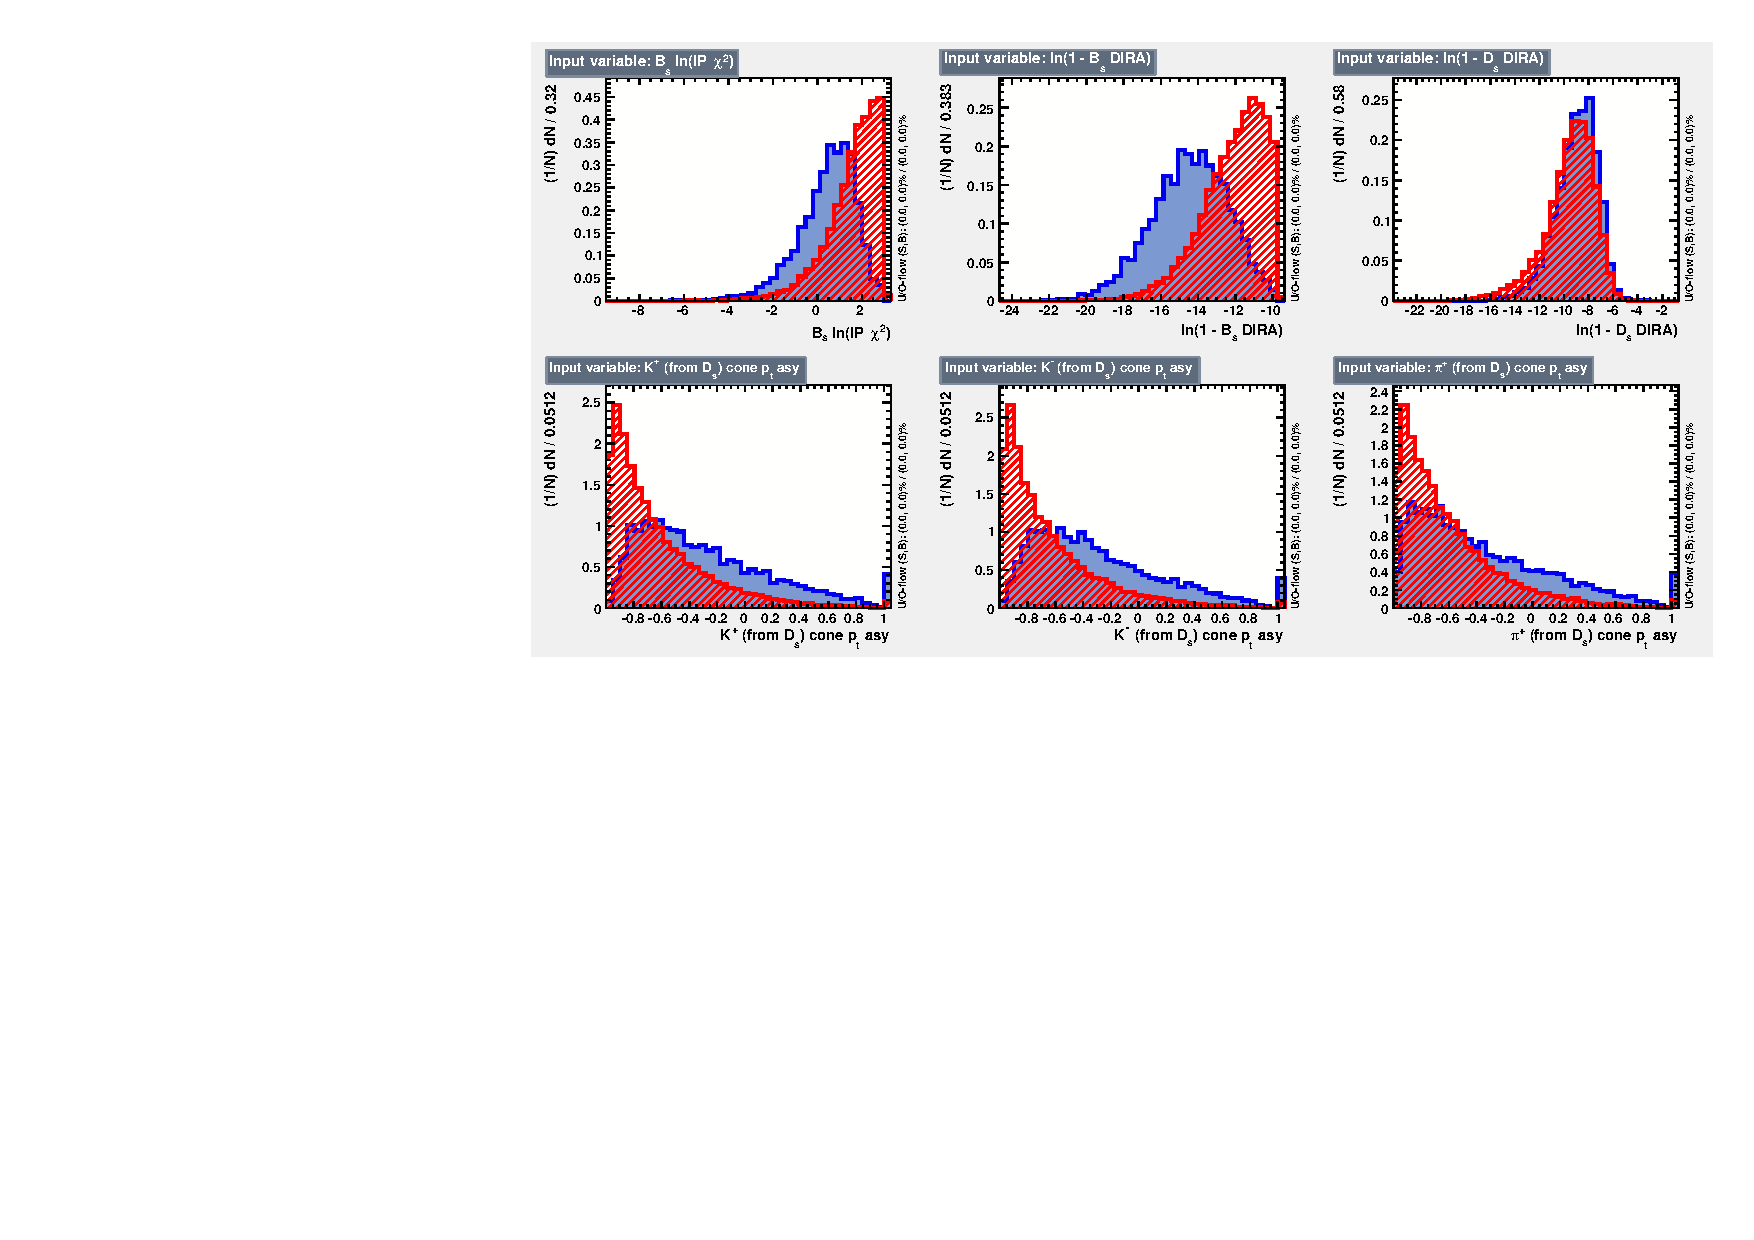
\includegraphics[height=6.cm,width=0.95\textwidth]{figs/BDT_Input_2.pdf}
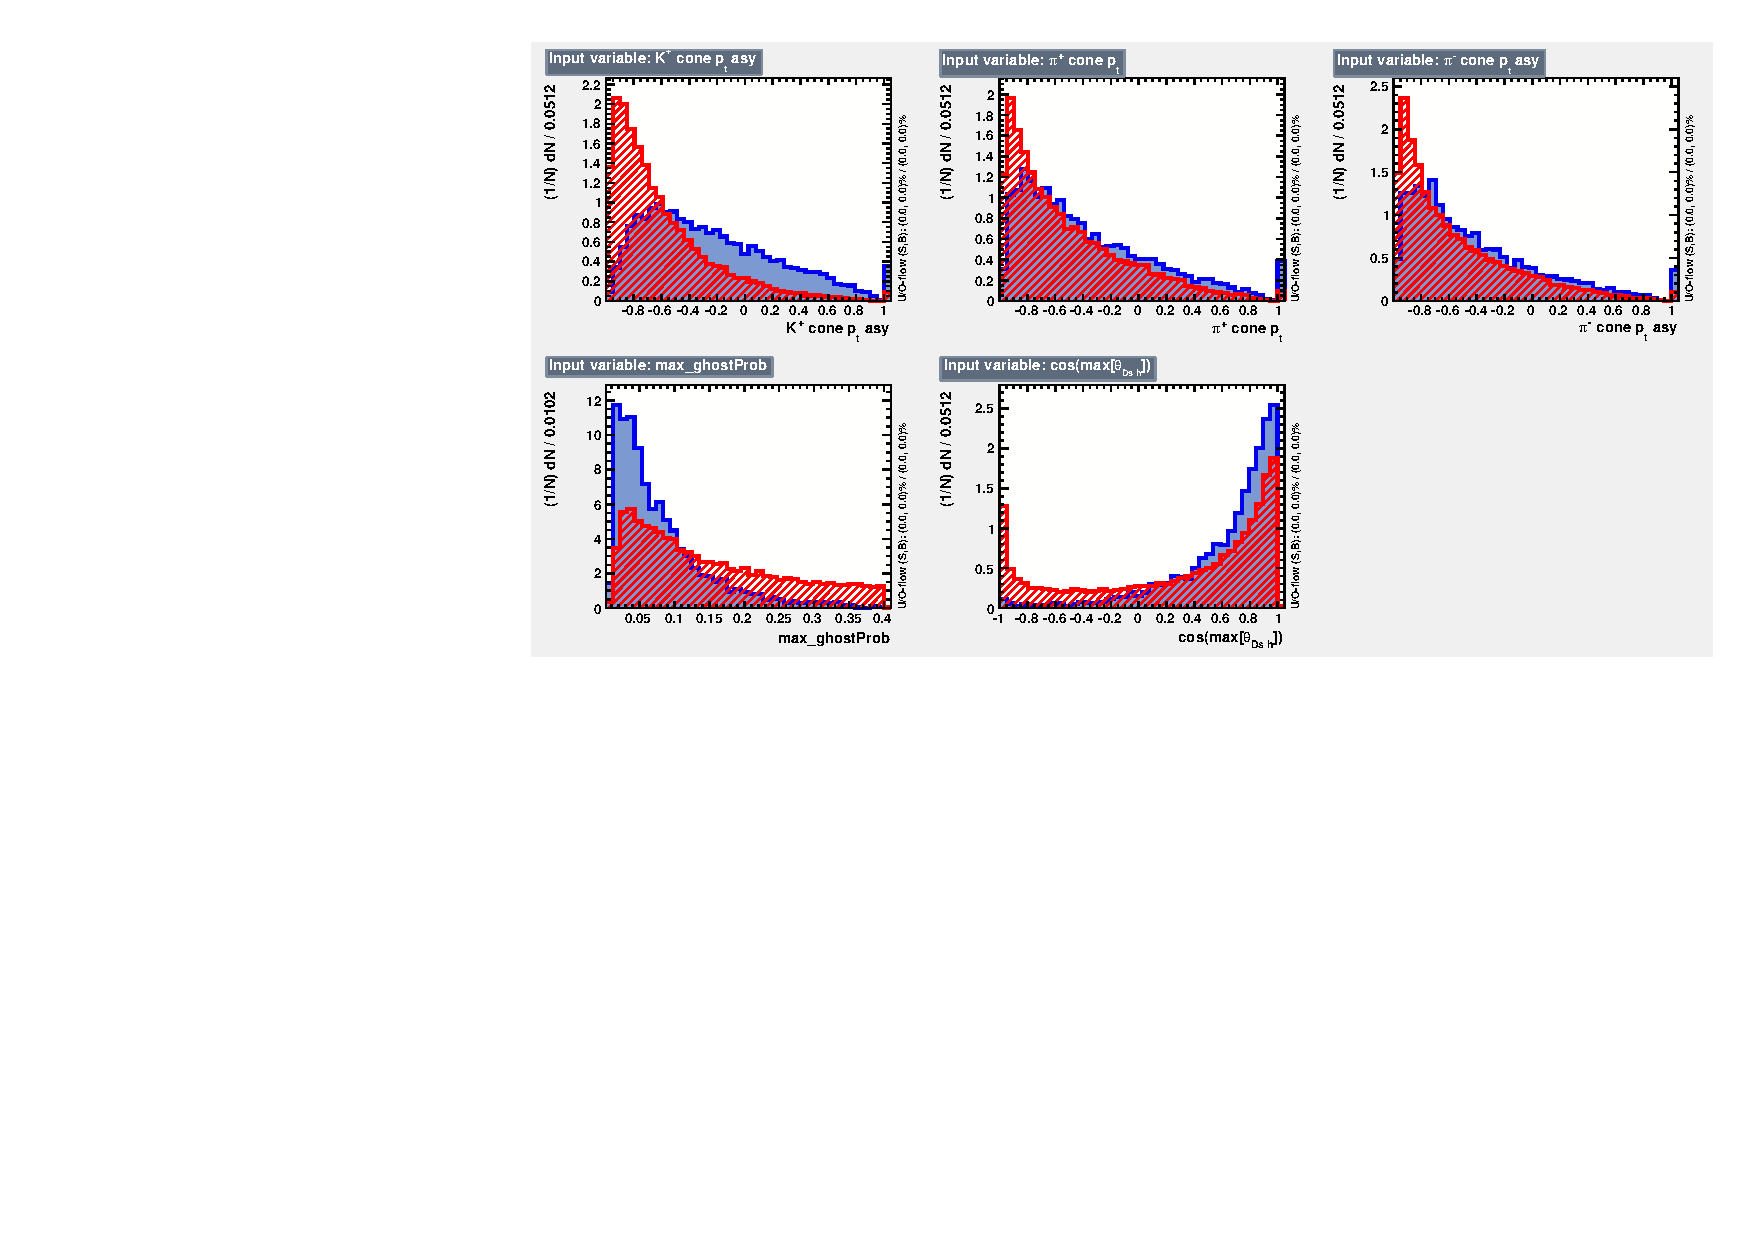
\includegraphics[height=6.cm,width=0.95\textwidth]{figs/BDT_Input_3.pdf}
%\vspace*{-0.2cm}
\caption{Distributions of the input variables used in the BDTG training. The background is shown as red hatched, while the signal is depicted solid blue.}
\label{fig:BDT_Input_1}
\end{figure}


The relative importance of the input variables for the BDTG training is summarized in Table \ref{table:InputVars}.

\begin{table}[h]
\centering
 \begin{tabular}{l c}
Variable & relative importance [$\%$]\\
  \hline
pi\_minus\_ptasy\_1.00 & 7.32\\
log\_Ds\_FDCHI2\_ORIVX & 7.23\\
K\_plus\_ptasy\_1.00 & 7.17\\
log\_Ds\_DIRA & 6.96\\
Bs\_ENDVERTEX\_CHI2 & 6.82\\
max\_ghostProb & 6.76\\
pi\_plus\_ptasy\_1.00 & 6.57\\
log\_DsDaughters\_min\_IPCHI2 & 6.21\\
log\_Bs\_DIRA & 6.15\\
K\_plus\_fromDs\_ptasy\_1.00 & 6.10\\
log\_XsDaughters\_min\_IPCHI2 & 5.87\\
K\_minus\_fromDs\_ptasy\_1.00 & 5.62\\
cos(Ds h) & 5.58\\
log\_Bs\_IPCHI2\_OWNPV & 5.08\\
log\_Bs\_FDCHI2\_OWNPV & 4.04\\
Xs\_max\_DOCA & 3.98\\
pi\_minus\_fromDs\_ptasy\_1.00 & 2.59\\
\end{tabular}
\caption{Summary of the relative importance of each variable in the training of the BDTG.}
\label{table:InputVars}
\end{table}

 
The BDTG output distribution for test and training samples is shown in Fig \ref{fig:BDT_Response}. No sign of overtraining is observed. 

\begin{figure}[h]
%\vspace*{-0.4cm}
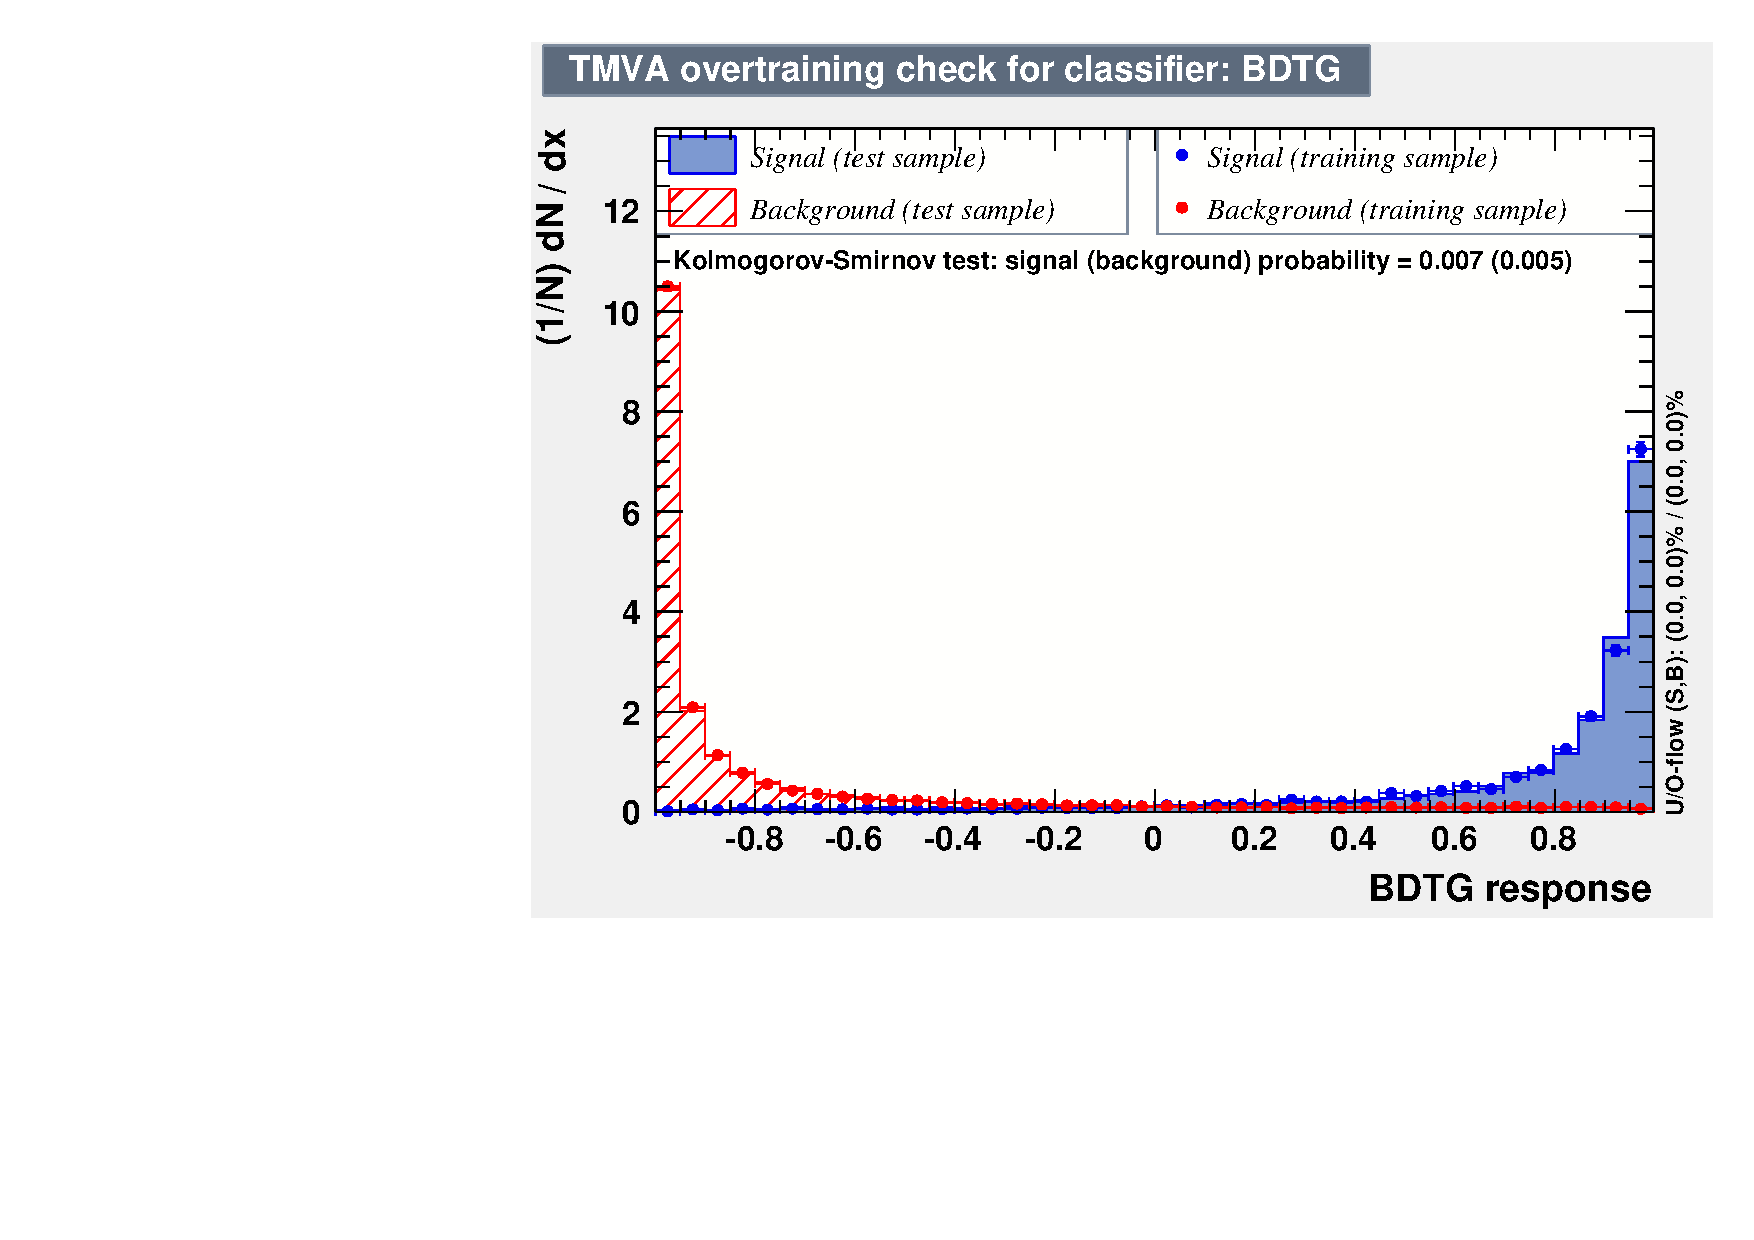
\includegraphics[height=7.4cm,width=0.7\textwidth]{figs/BDT_Response_new.pdf}
%\vspace*{-0.2cm}
\caption{BDTG output classifier distribution for (blue) signal and (red) background. The response of an independent test sample (dots) is overlaid.}
\label{fig:BDT_Response}
\end{figure}


       
We determine the optimal cut value by maximizing the figure of merit $S/\sqrt{S+B}$ where S is the signal yield and B the background yield in the signal region, defined to be within $\pm$50 $\mevcc$ of the nominal $\Bs$ mass. 
To avoid a bias in the determination of the branching fraction, we determine S and B using our normalization channel. 
All trigger, stripping and additional selection criteria described in this and the previous chapter are applied to the $\Bs\to\Ds\pion\pion\pion$ data samples. 
After that, we perform a simplified version of the fit to the invariant mass distribution of $\Bs\to\Ds\pion\pion\pion$ candidates described in Sec.~\ref{sec: fitting}.
Here, a Gaussian function to model the signal and an exponential function to model combinatorial background is used.
From this fit we estimate the number of signal events in our normalization channel. 
Multiplying that number with the PDG branching fraction of $\frac{\mathcal{B}(\Bs\to\Ds\kaon\pion\pion)}{\mathcal{B}(\Bs\to\Ds\pion\pion\pion)}$ and the ratio of efficiencies discussed in Sec. \ref{sec: efficiency} allows us to estimate the expected number of $\Bs\to\Ds\kaon\pion\pion$ signal decays. The number of background events can then be computed as

\begin{equation}
 N_{bkg}=N_{all}-N_{sig}|_{m_{\Bs\pm50\mevcc}}.   
\end{equation}

The efficiency curves as a function of the cut value are shown in Fig. \ref{fig:BDT_Efficiency}. 
The optimal cut value is found to be BDTG $>$ 0.7012. At this working point the signal efficiency is estimated to be 72.47 $\%$, while the background rejection in the signal region is 97.38 $\%$. 


\begin{figure}[h]
%\vspace*{-0.4cm}
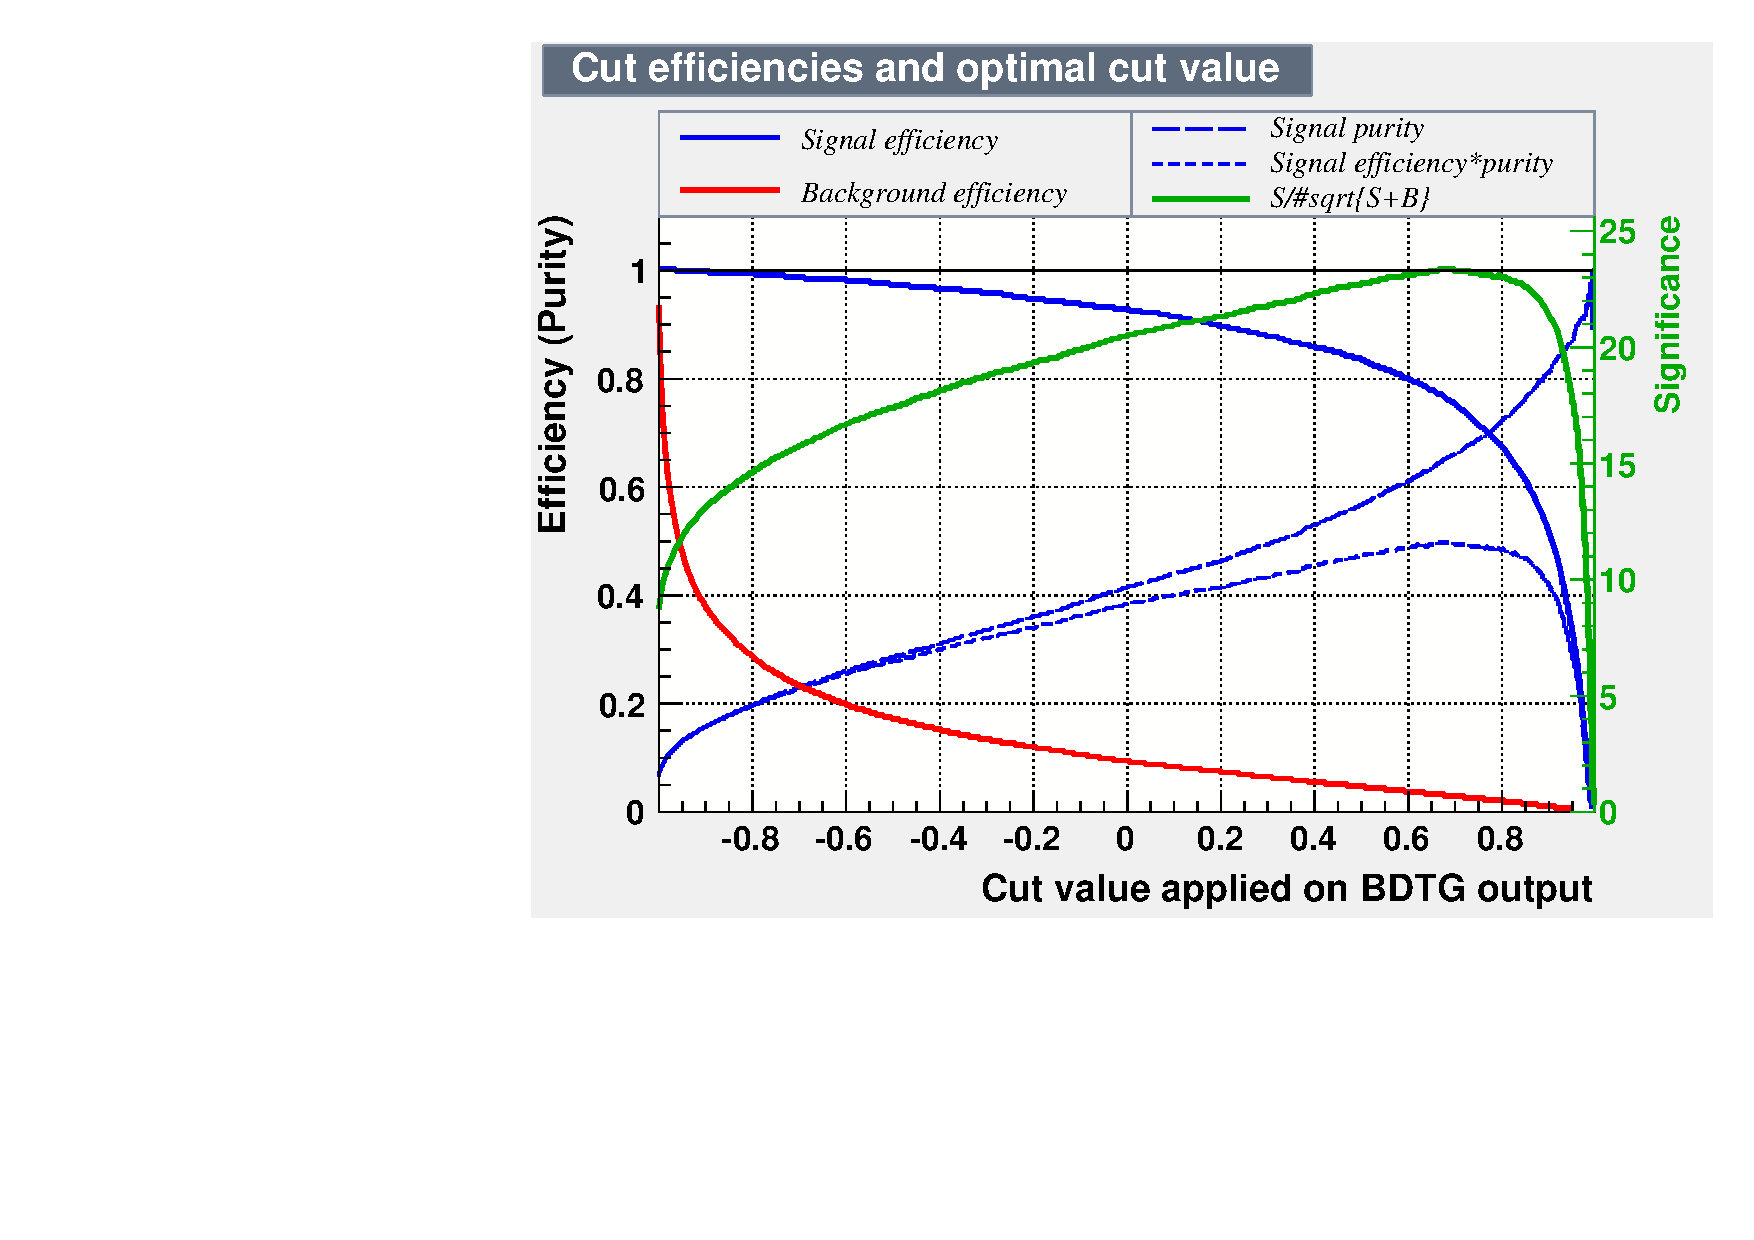
\includegraphics[height=7.4cm,width=0.7\textwidth]{figs/BDT_CutEfficiency.pdf}
%\vspace*{-0.2cm}
\caption{Efficiency and purity curves for (blue) signal, (red) background and the (green) FoM curve, as a function of the chosen cut value.}
\label{fig:BDT_Efficiency}
\end{figure}


\clearpage
% !TEX root = main.tex

\section{Yields determination}
\label{sec:massFits}

An extended unbinned maximum likelihood fit to the reconstructed $B_s$ mass of the selected events is performed in order to determine the signal and background yields.
The invariant mass $m(D_s h \pi \pi)$ is determined from a DTF constraining the mass of the $D_s$ to the PDG value and the position of the PV. 
The probability density functions (PDFs) used to describe the signal and background components are described in the following.

Due to different mass resolutions, we perform the invariant mass fits simultaneously for each data-taking period and each trigger category. 
We further introduce four $D_s$ final state categories:
$D_s \to \phi \pi$, $D_s \to K^*(892) \pi$, $D_s \to \pi \pi \pi$ and $D_s \to K h \pi$
to account for different signal purities. 
The $D_s \to K h \pi$ category combines the two $D_s$ decay channels with the lowest statistics: $D_s \to K K \pi$ (non-resonant) and $D_s \to K \pi \pi$.
This amounts to 16 categories in total.



\subsection{Signal model}
\label{subsec:signalModel}

The signal $B_s$-mass distribution of both $\Bs\to\Ds\kaon\pion\pion$ and $\Bs\to\Ds\pion\pion\pion$  is modeled using a Johnson's SU function \cite{10.2307/2332539}, which 
results from a variable transformation of a normal distribution to allow for asymmetric tails:
\begin{align}
\mathcal J(x\vert\mu,\sigma,\nu,\tau) &=
\frac{e^{- \frac{1}{2} r^2}}{2\pi \cdot c \cdot \sigma \cdot \tau \cdot \sqrt{z^2+1}} \\
% \frac{\delta}{\sigma 2\pi \sqrt{1+(\frac{m_{\Bs}-\mu}{\sigma})^{2}}} exp \left(-\frac{1}{2}[\gamma + \delta Argsh (\frac{m_{\Bs} - \mu}{\sigma})^{2}]\right).
r &= - \nu + \frac{\text{asinh}(z)}{\tau} \\
z & = \frac{x-(\mu - c \cdot \sigma \cdot e^\tau \text{sinh}(\nu\cdot \tau))}{c \cdot \tau} \\
c &= \frac{e^{\tau^2}-1}{2\sqrt{e^{\tau^2} \cdot \text{cosh}(2 \nu \cdot \tau)+1}} .
\label{eq:RooJohnsonSU}
\end{align}
It is conveniently expressed in terms of the central moments up to order four: 
The mean of the distribution $\mu$, the standard deviation $\sigma$,
the skewness $\nu$ and the kurtosis $\tau$.
%The sign of $\gamma$ in Eq. \ref{eq:RooJohnsonSU} determines whether the tail is located at lower ($\gamma > 0$) or higher ($\gamma < 0$) invariant mass values than the mean $\mu$ of the gaussian function 
%and $\delta$ describes the (a)symmetry of the fitted distribution. Higher values of $\delta$ result in a more symmetric, gaussian-like function.  
%Another Johnson SU function function is used to account for the contribution of the $\B^{0}\to\Ds\kaon\pion\pion$ decay, which is also present in the $m(\Ds\kaon\pion\pion)$ spectrum.
The tail parameters $\nu$ and $\tau$ are fixed to the values obtained by a fit to the invariant mass distribution of simulated events shown in Fig~\ref{fig: BsMassShapes}. 
\begin{figure}[h]
\centering
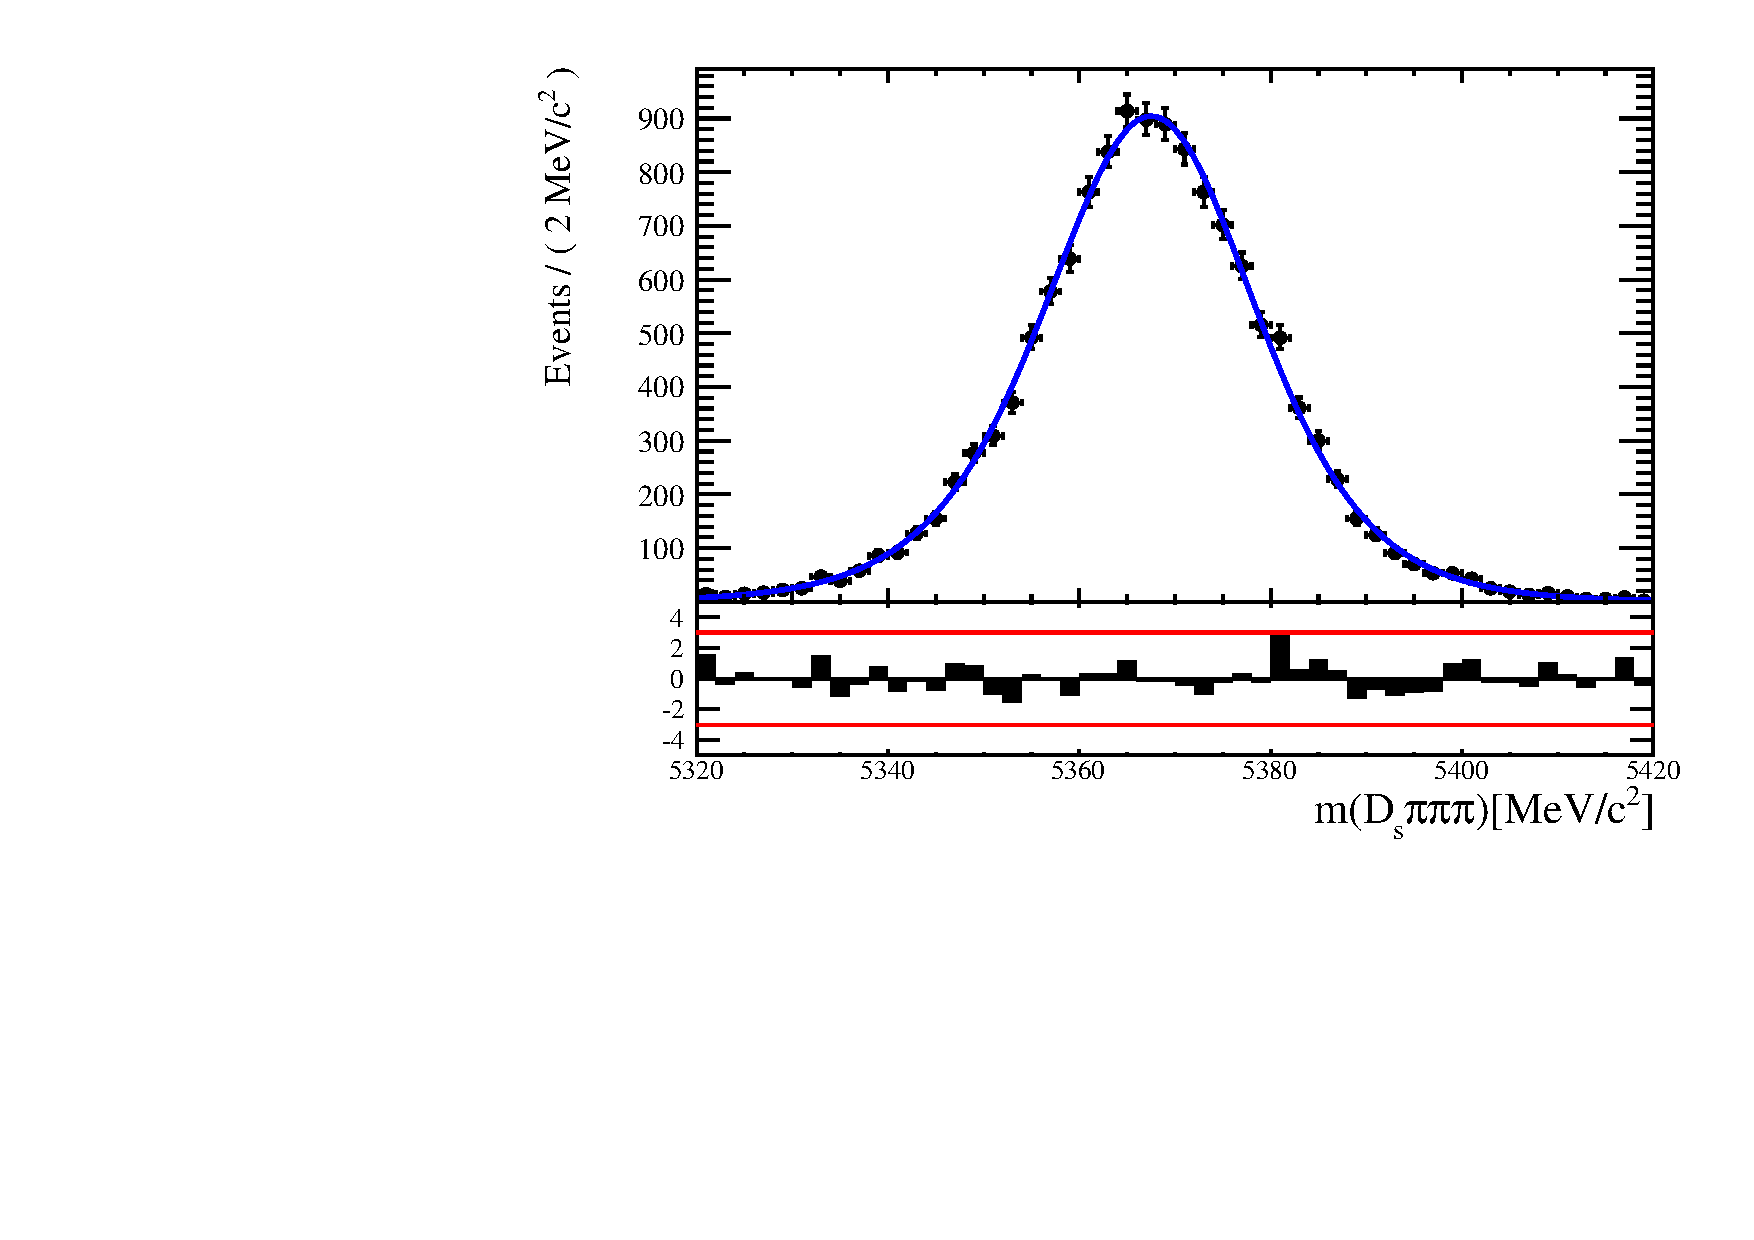
\includegraphics[height=!,width=0.45\textwidth]{figs/MassFit/normMC_pull.pdf} \hfill
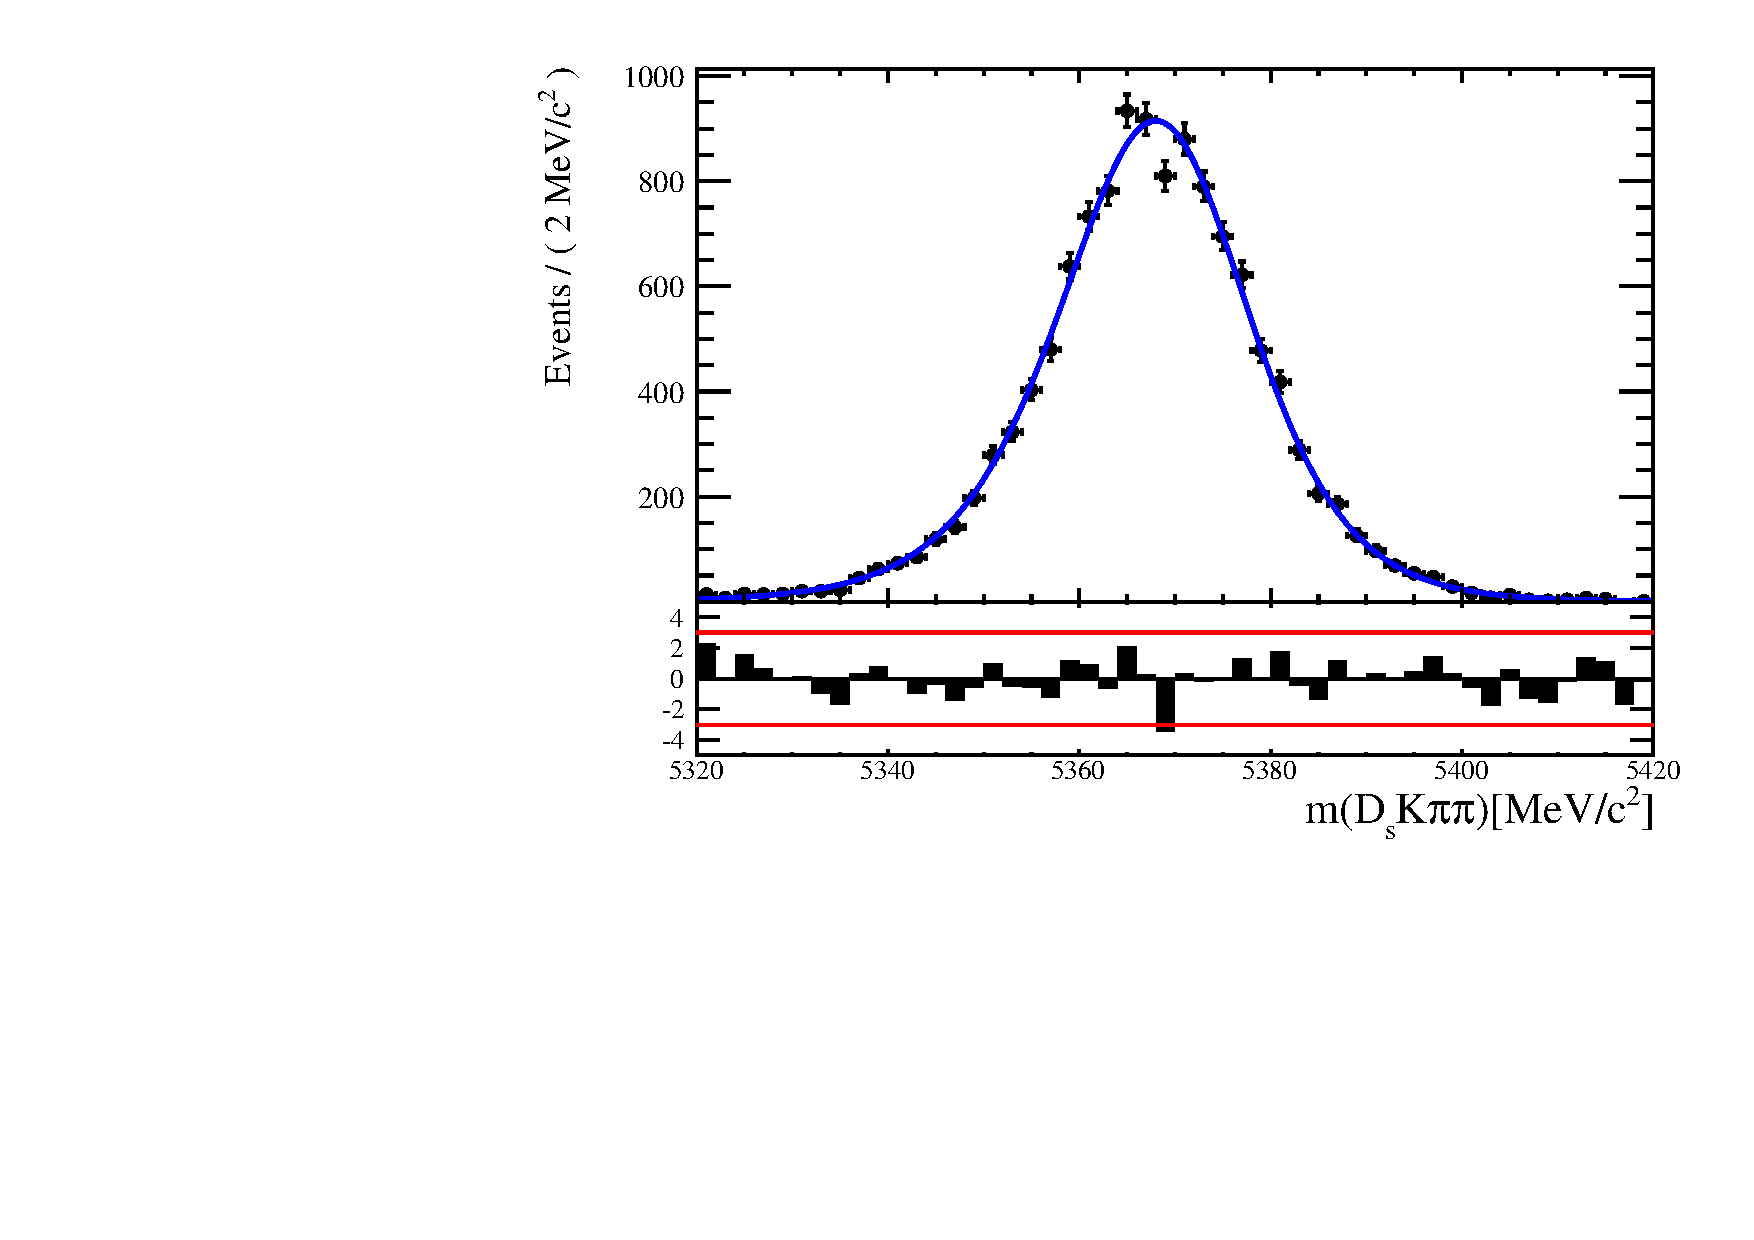
\includegraphics[height=!,width=0.45\textwidth]{figs/MassFit/signalMC_pull.pdf}
\caption{Invariant mass distributions of simulated (left) $\Bs\to\Ds\pion\pion\pion$ and (right) $\Bs\to\Ds\kaon\pion\pion$ events. A fit with a Johnson's SU PDF is overlaid.}
\label{fig: BsMassShapes}
\end{figure}
To account for differences between simulation and real data, linear scaling factors for the mean $\mu$ and width $\sigma$ are determined in the fit to $\Bs\to\Ds\pion\pion\pion$ data  
and later fixed in the fit to $\Bs\to\Ds\kaon\pion\pion$ decays. 
The scale factors are determined separately for each data-taking period and each trigger category.



\subsection{Background models} 
\label{subsec:bkgModel}

After the full selection the following residual background components have to be accounted for: \\

\noindent \textbf{Combinatorial background}  \\
The combinatorial background is described by a second order polynomial,
whose parameters are determined, for each $D_s$ final state separately, in the fit to data.
For systematic studies an exponential PDF is used.
\\

\noindent\textbf{Peaking $B_d$ background}  \\
Decays of $B_d$ mesons into the $D_s h \pi \pi$ final state are described by the $B_s$ signal PDF where the mean is shifted by the known mass difference $m_{B_s} - m_{B_d}$\cite{PDG2016}.
\\

\noindent \textbf{Partially reconstructed background}  \\
Partially reconstructed $\Bs\to D_s^{*}\pi\pion\pion$ decays, with $D_s^{*}\to\Ds\gamma$ or $D_s^{*}\to\Ds\piz$,
are expected to be peaking lower than signal in the $m(\Ds\pion\pion\pion)$ spectrum with large tails due to the %missing 
momentum carried away by the not reconstructed $\piz$ or $\gamma$. 
An empirical description for the shape of this contribution is derived from a $\Bs\to D_s^{*}\pi\pion\pion$ MC sample subject to the nominal $\Bs\to D_s\pi\pion\pion$ selection.
Figure \ref{fig:bgkShapes} (left) shows the respective reconstructed $m(D_s\pi\pi\pi)$ distribution.
A sum of three bifurcated Gaussian functions (\ie Gaussian functions with different widths on the left and the right side of the maximum value) is used to describe it.
In the fit to data, all parameters are fixed to the ones obtained from MC except for the parameter which describes the width of the right tail of the distribution to account for
data-simulation differences in mass resolution.
The equivalent $\Bs\to D_s^{*}K\pion\pion$ component contributing to the $\Bs\to D_s K\pion\pion$ data sample is described by the same PDF with the right tail fixed to the 
$\Bs\to D_s \pi\pion\pion$ result.

Contributions from $\Bz\to D_s^{*}K\pion\pion$ decays are modeled with the $\Bs\to D_s^{*}K\pion\pion$ PDF  shifted by $m_{\Bs} - m_{\Bz}$. \\
%Contributions from $\Bz\to D_s^{*}h\pion\pion$ decays where initially considered as well (modeled with the same PDF as $\Bs\to D_s^{*}h\pion\pion$ decays shifted by $m_{\Bs} - m_{\Bz}$) but were found to be negligible within the considered mass range. \\
%The yields of both contributions are directly determined in the nominal fit. \\

\noindent\textbf{Misidentified background}  \\
A small fraction of $B_s \to D_s^- \pi^+ \pi^+ \pi^-$ and $\Bs\to D_s^{*}\pi^+ \pi^+ \pi^-$ decays, where one of the pions is misidentified as a kaon, contaminate the 
$\Bs\to D_s K^+ \pi^+ \pi^-$ sample.
To determine the corresponding background shapes, we use simulated events passing the nominal selection
except for the PID cuts on the bachelor $\pi^+$ tracks. 
The \textsf{PIDCalib} package is used to determine the $p_T,\eta$-dependent $\pi^+\rightarrow K^+$ misidentification probability for each pion. 
%For every candidate in our MC sample, a (momentum) $\ptot$ and (pseudorapidity) $\eta$-dependent event weight is computed and assigned. 
We change the particle hypothesis from pion to kaon for the pion with the higher misidentification probability and recompute the invariant $\Bs$ mass, $m(D_s^- \pi^+_K \pi^+ \pi^- )$. 
Similarly, the invariant masses $m(\pi^+_K \pi^+ \pi^- )$ and $m(\pi^+_K \pi^-)$ are recomputed and required to be within the considered phasespace region.
The background distributions are shown in Fig.~\ref{fig:bgkShapes} (middle,right) and modeled by the sum of two Crystal Ball functions. 
The expected yield of misidentified $\Bs\to\Ds\pion\pion\pion$ ($\Bs\to D_s^{*}\pi^+ \pi^+ \pi^-$) candidates in the $\Bs\to\Ds K\pion\pion$ sample is computed 
by multiplying the fake rate (within the considered $B_s$ mass range) of $0.47\%$ ($0.61\%$) %, which is derived from \textsf{PIDCalib}, 
by the $\Bs\to\Ds\pion\pion\pion$ ($\Bs\to D_s^{*}\pi^+ \pi^+ \pi^-$) yield as determined in the mass fit to the $\Bs\to\Ds\pion\pion\pion$ data sample which is 
corrected for the PID($\pip$)$<0$ requirement.  
The $\Bs\to D_s^{*}\pi^+ \pi^+ \pi^-$ yield is additionally corrected for the efficiency of the cut $m(\Ds K\pion\pion)>5200\mev$ evaluated on MC.
In the fit to data, the misidentified background yields are fixed to the predicted ones.
%In the same way as mentioned above, we can determine the rate of misidentified, partially reconstructed $\Bs\to\Ds^{*}\pion\pion\pion$ decays in our sample of $\Bs\to\Ds\kaon\pion\pion$ decays using \textsf{PIDCalib} and a MC sample of $\Bs\to\Ds^{*}\pion\pion\pion$ events. The invariant mass distribution we obtain when we exclude the $\gamma$/$\piz$, flip the the particle hypothesis $\pion\rightarrow\kaon$ and apply the event weights given by the fake rate, is shown in Fig.~\ref{fig:bgkShapes} (right). 
%The fit of two Crystal Ball functions to this distribution is overlaid. 
%The yield of this contribution is determined from the yield of $\Bs\to\Ds^{*}\pion\pion\pion$ candidates in the nominal mass fit of our normalization channel, multiplied by the misID probability of $\propto 3.6\%$.

We consider the $\Bs\to D_s K\pion\pion$ and $\Bs\to D_s^{*}K\pion\pion$ components contributing to the $\Bs\to D_s \pi\pion\pion$ data sample to be negligible 
due to the low branching fractions and the tight PID cuts on the bachelor pions.

\begin{figure}[t]
\centering
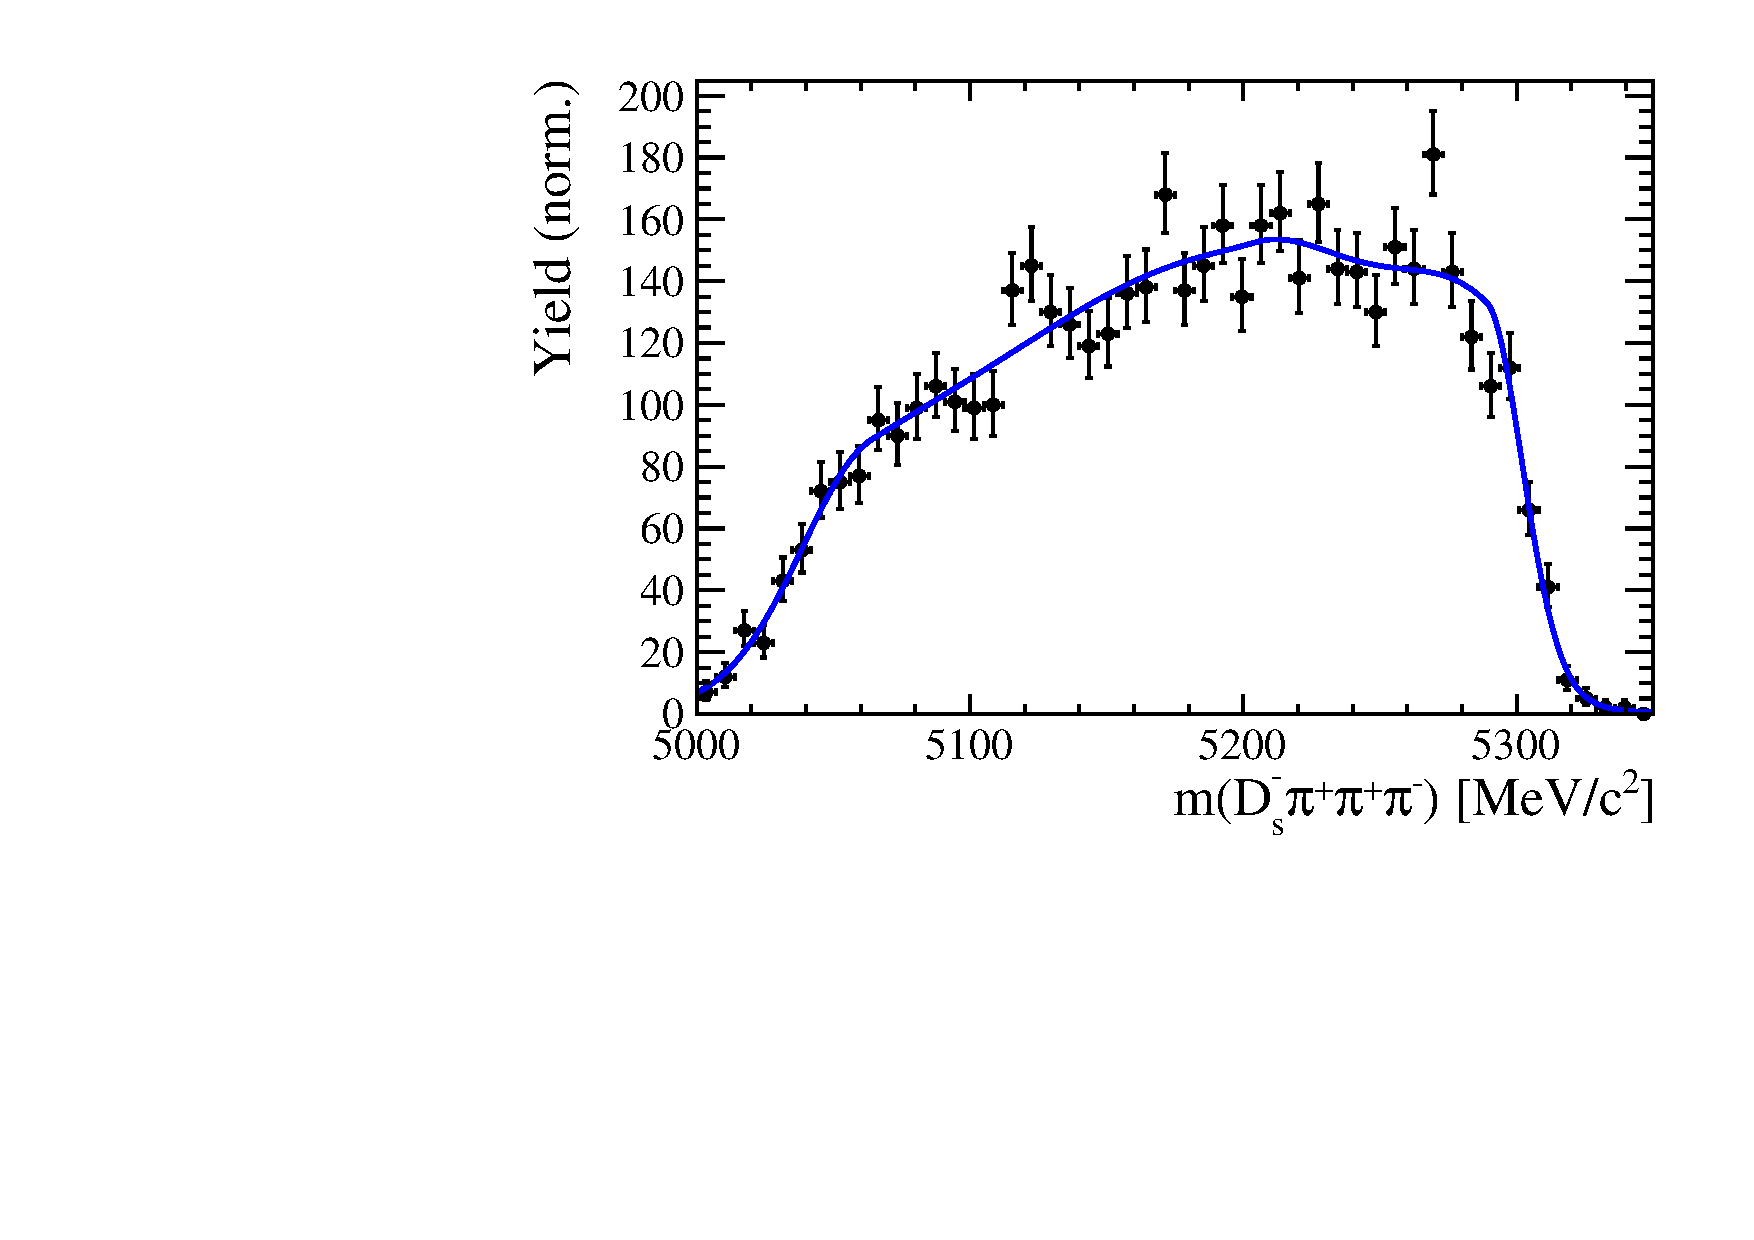
\includegraphics[height=!,width=0.32\textwidth]{figs/MassFit/BkgShape/Bs2Dsstartpipipi.pdf}
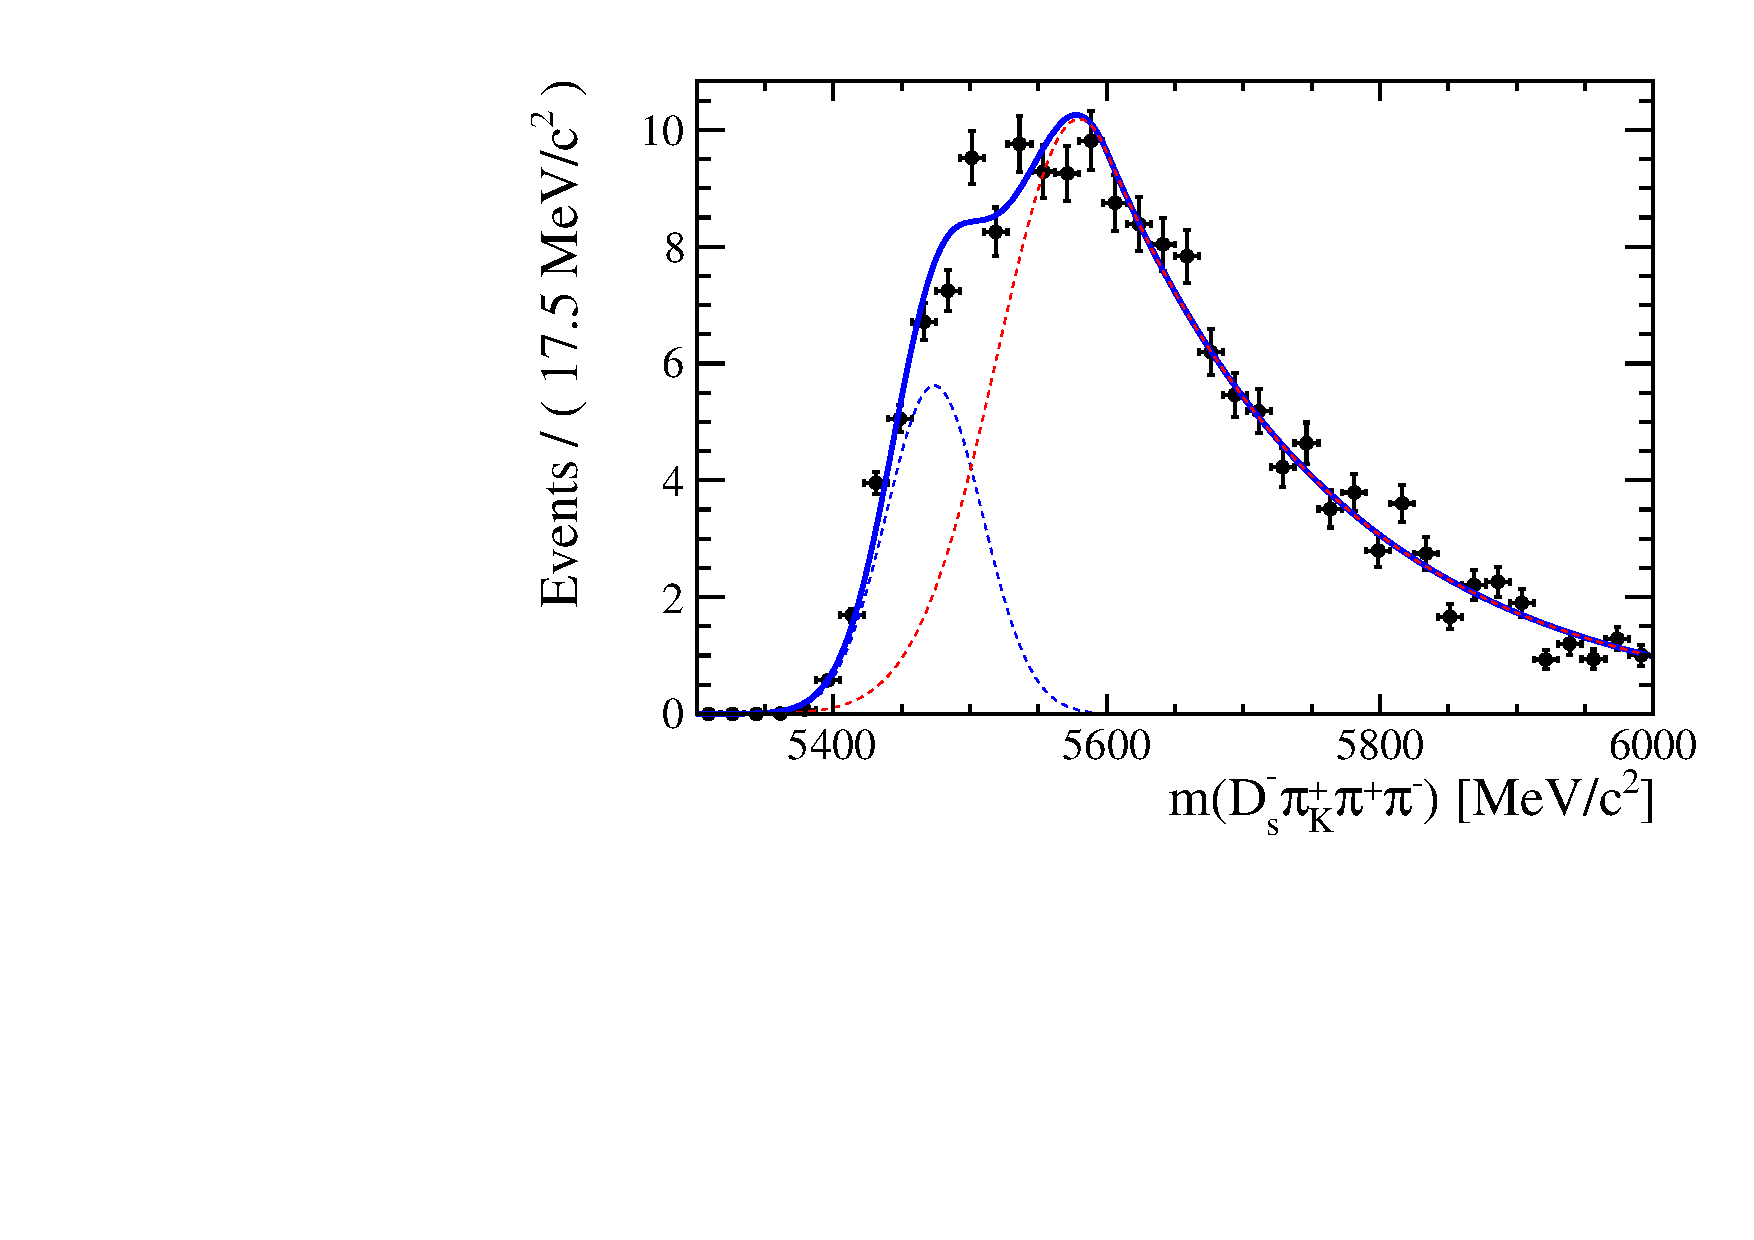
\includegraphics[height=!,width=0.32\textwidth]{figs/MassFit/BkgShape/Bs2Dspipipi_as_DsKpipi.pdf}
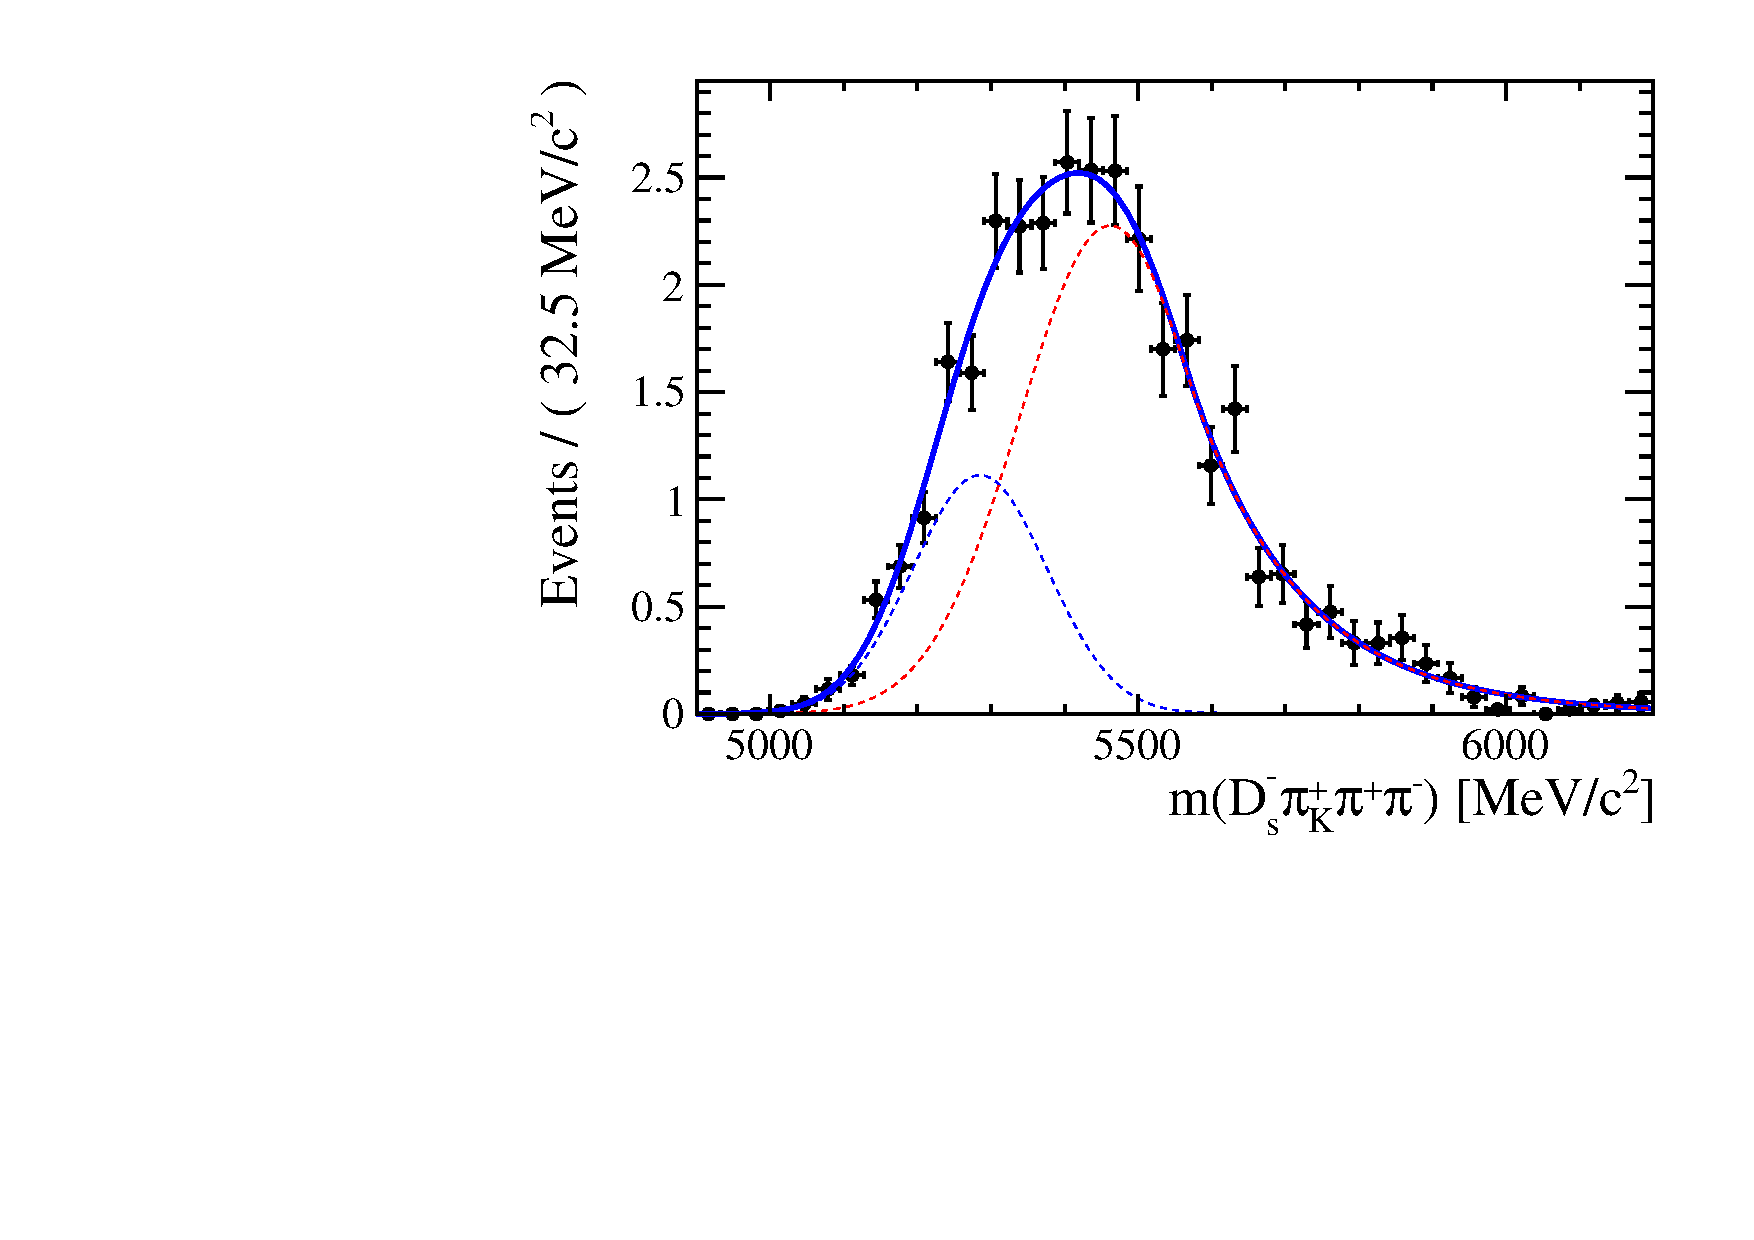
\includegraphics[height=!,width=0.32\textwidth]{figs/MassFit/BkgShape/Bs2Dsstarpipipi_as_DsKpipi.pdf}
\caption{
Left: Invariant mass distribution of simulated $\Bs\to D_s^{*}\pion\pion\pion$ events, where the $\gamma$/$\piz$ is excluded from the reconstruction. 
Middle: Invariant mass distribution of  simulated $\Bs\to\Ds\pion\pion\pion$ events, where one of the pions is reconstructed as a kaon taking the misidentification probability into account. 
Right: Invariant mass distribution for simulated $\Bs\to D_s^{*}\pion\pion\pion$ events, where the $\gamma$/$\piz$ from the $D_s^{*}$ is excluded from reconstruction
and one of the pions is reconstructed as a kaon taking the misidentification probability into account. The fitted PDF is shown in blue.}
\label{fig:bgkShapes}
\end{figure}
 

\subsection{Results}
\label{subsec:Results}

Figure \ref{fig:massFit} shows the invariant mass distribution for $\Bs\to\Ds\pion\pion\pion$ and  $\Bs\to\Ds\kaon\pion\pion$ candidates passing all selection criteria.
The projections for all categories of the simultaneous fit are shown in Appendix \ref{sec:DetailedMassfits} together with the results for all fitted parameters.
The integrated signal and background yields are listed in Tables \ref{tab:massFitNorm} and \ref{tab:massFitSig}.

\begin{figure}[h]
\centering
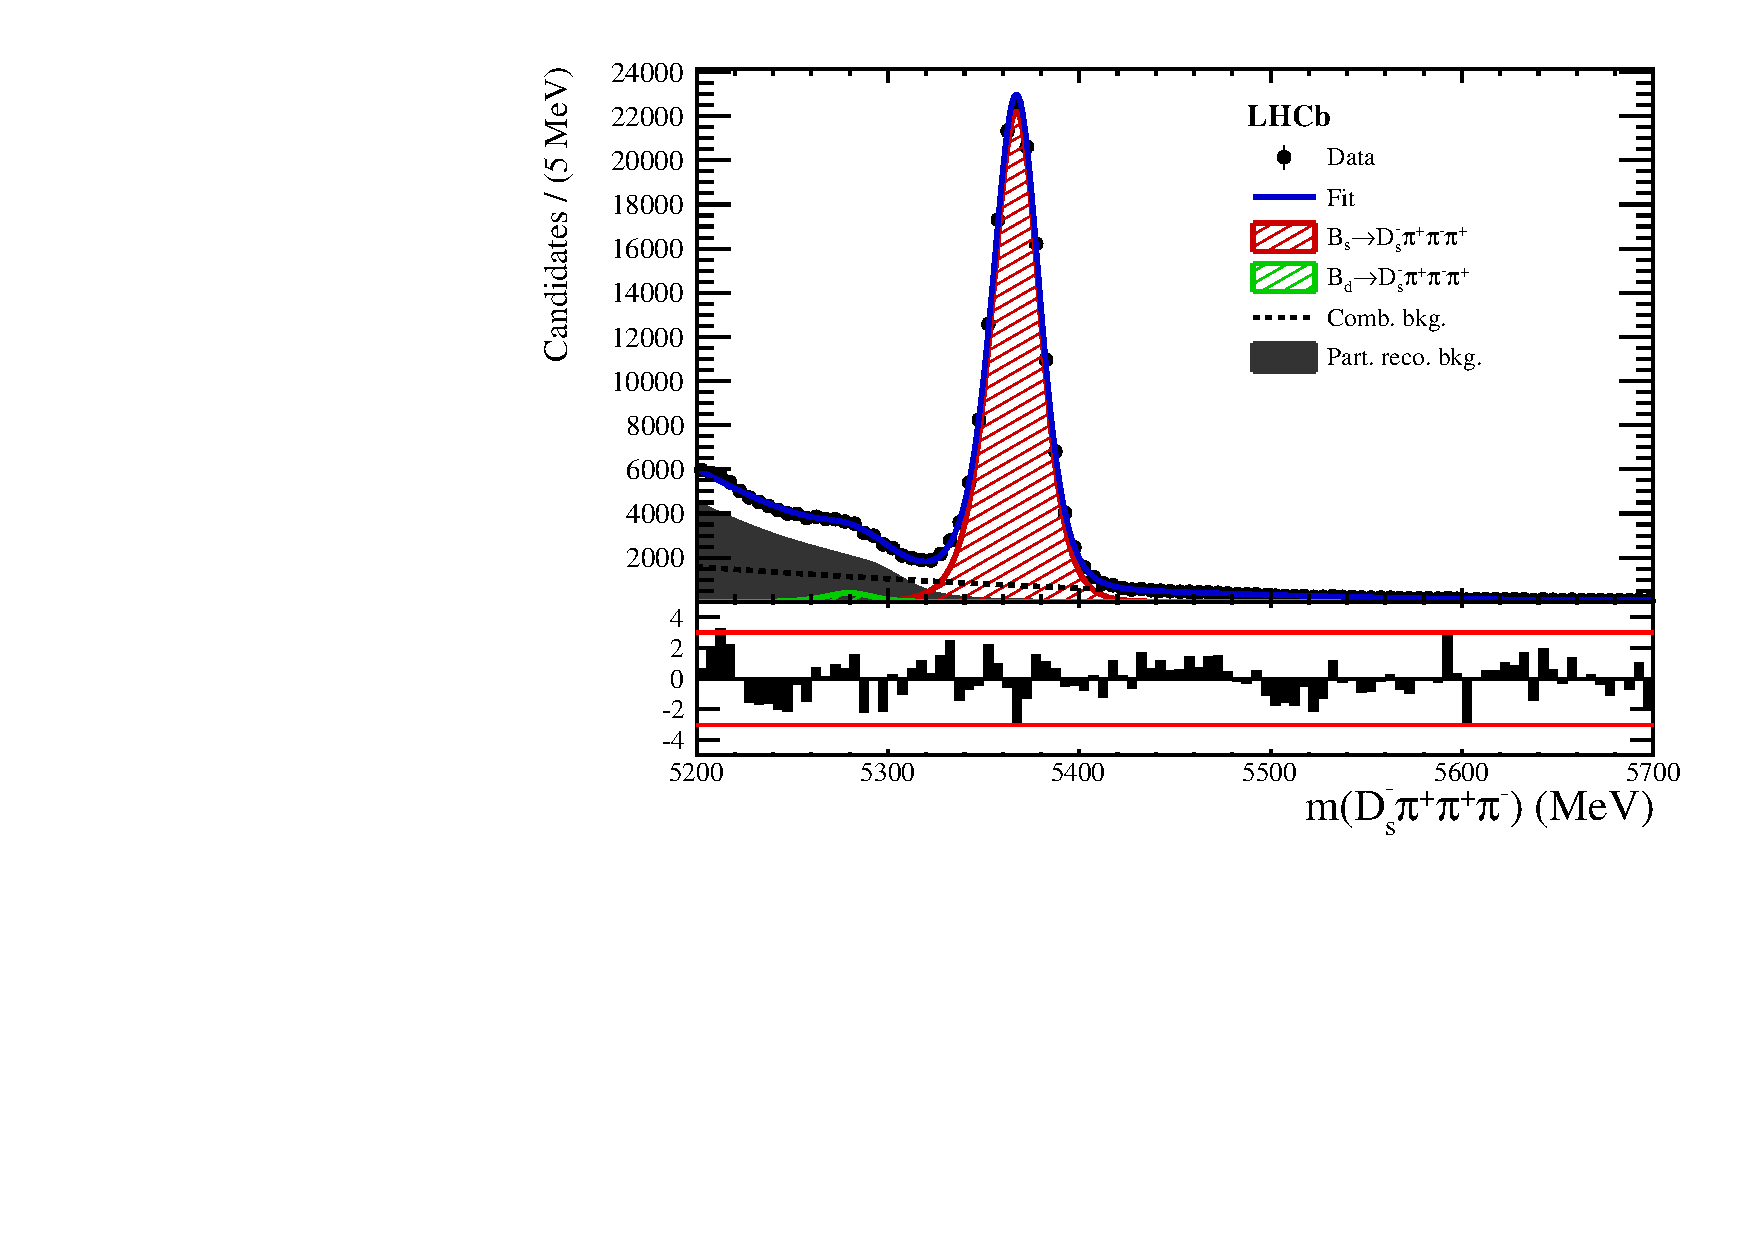
\includegraphics[height=!,width=0.49\textwidth]{figs/MassFit/norm_pull.pdf}
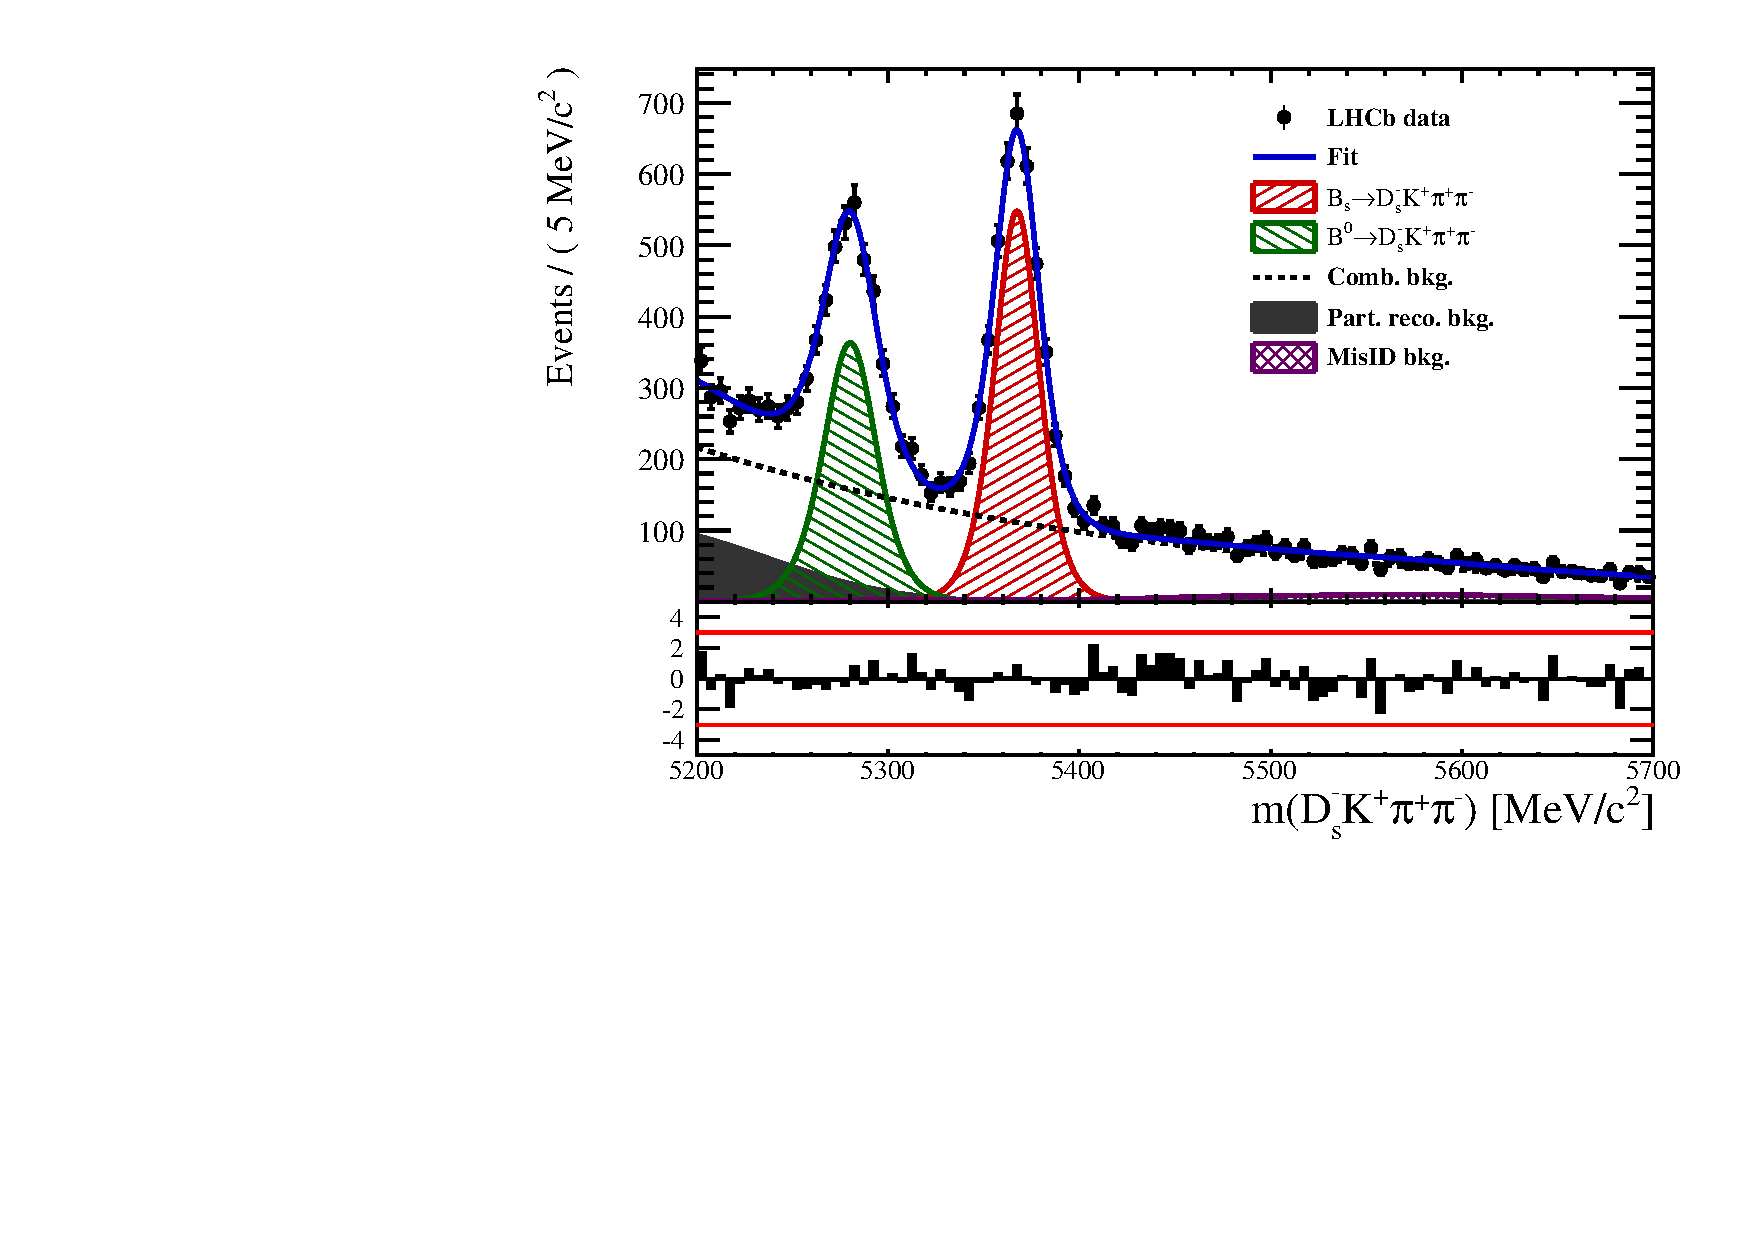
\includegraphics[height=!,width=0.49\textwidth]{figs/MassFit/signal_pull.pdf}
\caption{Invariant mass distribution of $\Bs\to\Ds\pion\pion\pion$ (left) and  $\Bs\to\Ds\kaon\pion\pion$ (right) candidates.}
\label{fig:massFit}
\end{figure}

\clearpage
\begin{table}[h]
\centering
\caption{Total signal and background yields for the $B_s \to D_s \pi \pi \pi$ sample (left) and
signal yield for the different $D_s$ final states contributing to the $B_s \to D_s \pi \pi \pi$ sample (right).}
 \begin{tabular}{l r }
\hline\hline
Component & Yield\ \\
\hline
$B_s \to D_s \pi \pi \pi$ & 77225 $\pm$ 304 \\
$B^{0} \to D_s \pi \pi \pi$ & 1263 $\pm$ 454 \\
Partially reconstructed bkg. & 31805 $\pm$ 351 \\
Combinatorial bkg. & 32821 $\pm$ 393 \\
\hline\hline
\end{tabular}
\label{table:normYields}
 \hfill
 \begin{tabular}{l r }
\hline\hline
$D_s$ final state  & Signal yield\ \\
\hline
$D_{s}^{-} \to \phi^{0}(1020)\pi^{-}$ & 34563 $\pm$ 197 \\
$D_{s}^{-}\to K^{*0}(892)K^{-}$ & 28472 $\pm$ 189 \\
$D_{s}^{-}\to (K^{-}h^{+}\pi^{-})$ & 21047 $\pm$ 160 \\
$D_{s}^{-}\to \pi^{+}\pi^{-}\pi^{-}$ & 17208 $\pm$ 145 \\
\hline\hline
\end{tabular}
\label{table:normYieldsDs}

\label{tab:massFitNorm}
\end{table}
\begin{table}[h]
\centering
\caption{Total signal and background yields for the $B_s \to D_s K \pi \pi$ sample (left) and
signal yield for the different $D_s$ final states contributing to the $B_s \to D_s  K \pi \pi$ sample (right).}
 \begin{tabular}{l r }
\hline\hline
Component & Yield\ \\
\hline
$B_s \to D_s K \pi \pi$ & 5376 $\pm$ 88 \\
$B^{0} \to D_s K \pi \pi$ & 4384 $\pm$ 101 \\
Partially reconstructed bkg. & 1796 $\pm$ 96 \\
Misidentified bkg. & 808 $\pm$ 0 \\
Combinatorial bkg. & 9376 $\pm$ 177 \\
\hline\hline
\end{tabular}
\label{table:signalYields}
 \hfill
 \begin{tabular}{l r }
\hline\hline
$D_s$ final state  & Signal yield\ \\
\hline
$D_{s}^{-} \to \phi^{0}(1020)\pi^{-}$ & 1728 $\pm$ 49 \\
$D_{s}^{-}\to K^{*0}(892)K^{-}$ & 1575 $\pm$ 47 \\
$D_{s}^{-}\to (K^{-}h^{+}\pi^{-})$ & 1166 $\pm$ 41 \\
$D_{s}^{-}\to \pi^{+}\pi^{-}\pi^{-}$ & 823 $\pm$ 37 \\
\hline\hline
\end{tabular}
\label{table:signalYieldsDs}

\label{tab:massFitSig}
\end{table}




\clearpage
% !TEX root = main.tex
\clearpage
\section{Flavour Tagging}
\label{sec:Tagging}

To identify the initial flavour state of the $\Bs$ meson,
a number of flavour tagging algorithms are used that either determine the flavour of the non-signal b-hadron produced in the event (opposite site, OS)
or use particles produced in the fragmentation of the signal candidate $\Bs$/$\Bsb$ (same side, SS). 

For the same side, the algorithm searching for the charge of an additional kaon that accompanies the fragmentation of the signal candidate is used (SS-nnetKaon). 
For the opposite site, four different taggers are chosen: 
The algorithms that use the charge of an electron or a muon from semileptonic B decays (OS- $\electron$,$\muon$), the tagger that uses the charge of a kaon from a b $\to$ c $\to$ s decay chain (OS-nnetKaon) 
and the algorithm that determines the $\Bs$/$\Bsb$ candidate flavour from the charge of a secondary vertex, reconstructed from the OS b decay product (OS-VtxCharge). 
All four taggers are then combined into a single OS tagger. 

Every single tagging algorithm is prone to misidentify the signal candidate at a certain mistag rate $\omega = (wrong tags)/ (all tags)$. 
This might be caused by particle misidentification, flavour oscillation of the neutral opposite site B-meson or by tracks that are wrongly picked up from the underlying event. 
For every signal $\Bs$/$\Bsb$ candidate, each tagging algorithm predicts a mistag probability $\eta$, which is calculated using a combination of inputs such as the kinematics of the tagging particles. 
The inputs are then combined to a predicted mistag using neural networks. These are trained on simulated samples of $\Bs\to\Dsm\pip$ (SS algorithm) and $\Bu\to\jpsi\Kp$ (OS algorithms) decays.
For the presented analysis, the measurable CP-violating coefficients are damped by the tagging dilution $D$, that depends on the mistag rate:
\begin{equation}
\label{eq: taggingDilution}
D = 1 - 2\omega.
\end{equation}
This means that the statistical precision, with which these coefficients can be measured, scales as the inverse square root of the effective tagging efficiency,
\begin{equation}
\label{eq: taggingEfficiency}
\epsilon_{eff} = \epsilon_{tag}(1 - 2\omega)^{2},
\end{equation}
where $epsilon_{tag}$ is the fraction of events that have a tagging decision. 
The flavour tagging algorithms are optimized for highest $\epsilon_{eff}$ on data, using the $\Bs\to\Dsm\pip$ and $\Bu\to\jpsi\Kp$ samples. \newline
Utilizing flavour-specific final states, the predicted mistag $\eta$ of each tagger has to be calibrated to match the observed mistag $\omega$ on the data sample. 
For the calibration, a linear model of the form
\begin{equation}
\label{eq: mistagCalibration}
\omega(\eta) = p_{o} + p_{1} \cdot (\eta - < \eta >), 
\end{equation}  
where the values of $p_{0}$ and $p_{1}$ are determined using the $\Bs\to\Ds\pion\pion\pion$ normalization mode and $<\eta>$ is the average estimated mistag probability $<\eta> = \Sigma_{i=1}^{N_{cand}}(\eta_{i}) / N_{cand}$.
Following this model, a perfectly calibrated tagger would lead to $\omega(\eta) = \eta$ and one would expect $p_{1} = 1$ and $p_{0} = <\eta>$.
Due to the different interaction cross-sections of oppositely charged particles, the tagging calibration parameters depend on the initial state flavour of the $\Bs$. 
Therefore, the flavour asymmetry parameters $\Delta p_{0}$, $\Delta p_{1}$ and $\Delta\epsilon_{tag}$ are introduced. 
For this analysis, the calibrated mistag is treated as per-event variable, giving a larger weight to events that are less likely to have an incorrect tag. 
This adds one additional observable to the time- and amplitude-dependent fit. \newline
The tagging calibration is determined using a time-dependent fit to the full $\Bs\to\Ds\pion\pion\pion$ sample, where the mixing frequency $\dms$ is fixed to the nominal PDG value \cite{PDG2014}.
The calibration procedure for the OS tagging algorithms (Sec.\ref{subsec: OScalibration}) and 
the SS kaon tagger (Sec.\ref{subsec: SScalibration}) is applied on the full Run I and 2015 and 2016 Run II $\Bs\to\Ds\pion\pion\pion$ data sample, which is selected following the steps described in Sec. \ref{sec:Selection}.
The similar selection ensures as close as possible agreement between the $\Bs\to\Ds\pion\pion\pion$ and $\Bs\to\Ds\kaon\pion\pion$ samples in terms of the decay kinematics, which are crucial for the flavour tagging.
Section \ref{subsec: TaggingComparison} shows the compatibility of both samples. After applying the calibration, the response of the OS and SS taggers are combined, which is shown in Sec. \ref{subsec: TaggingCombination}.  



\subsection{OS tagging calibration}
\label{subsec: OScalibration}
The responses of the OS electron, muon, neural net kaon and the secondary vertex charge taggers are combined for the mistag calibration. 
Figure \ref{fig:OSdistribution} shows the distribution of the predicted OS mistag for signal candidates from $\Bs\to\Ds\pion\pion\pion$. 
The extracted calibration parameters and tagging asymmetries are summarized in Table \ref{table: OScalibration} and the measured tagging power for the OS combination is $\epsilon_{eff,OS} = 4.81 \%$.


\begin{figure}[h]
\centering
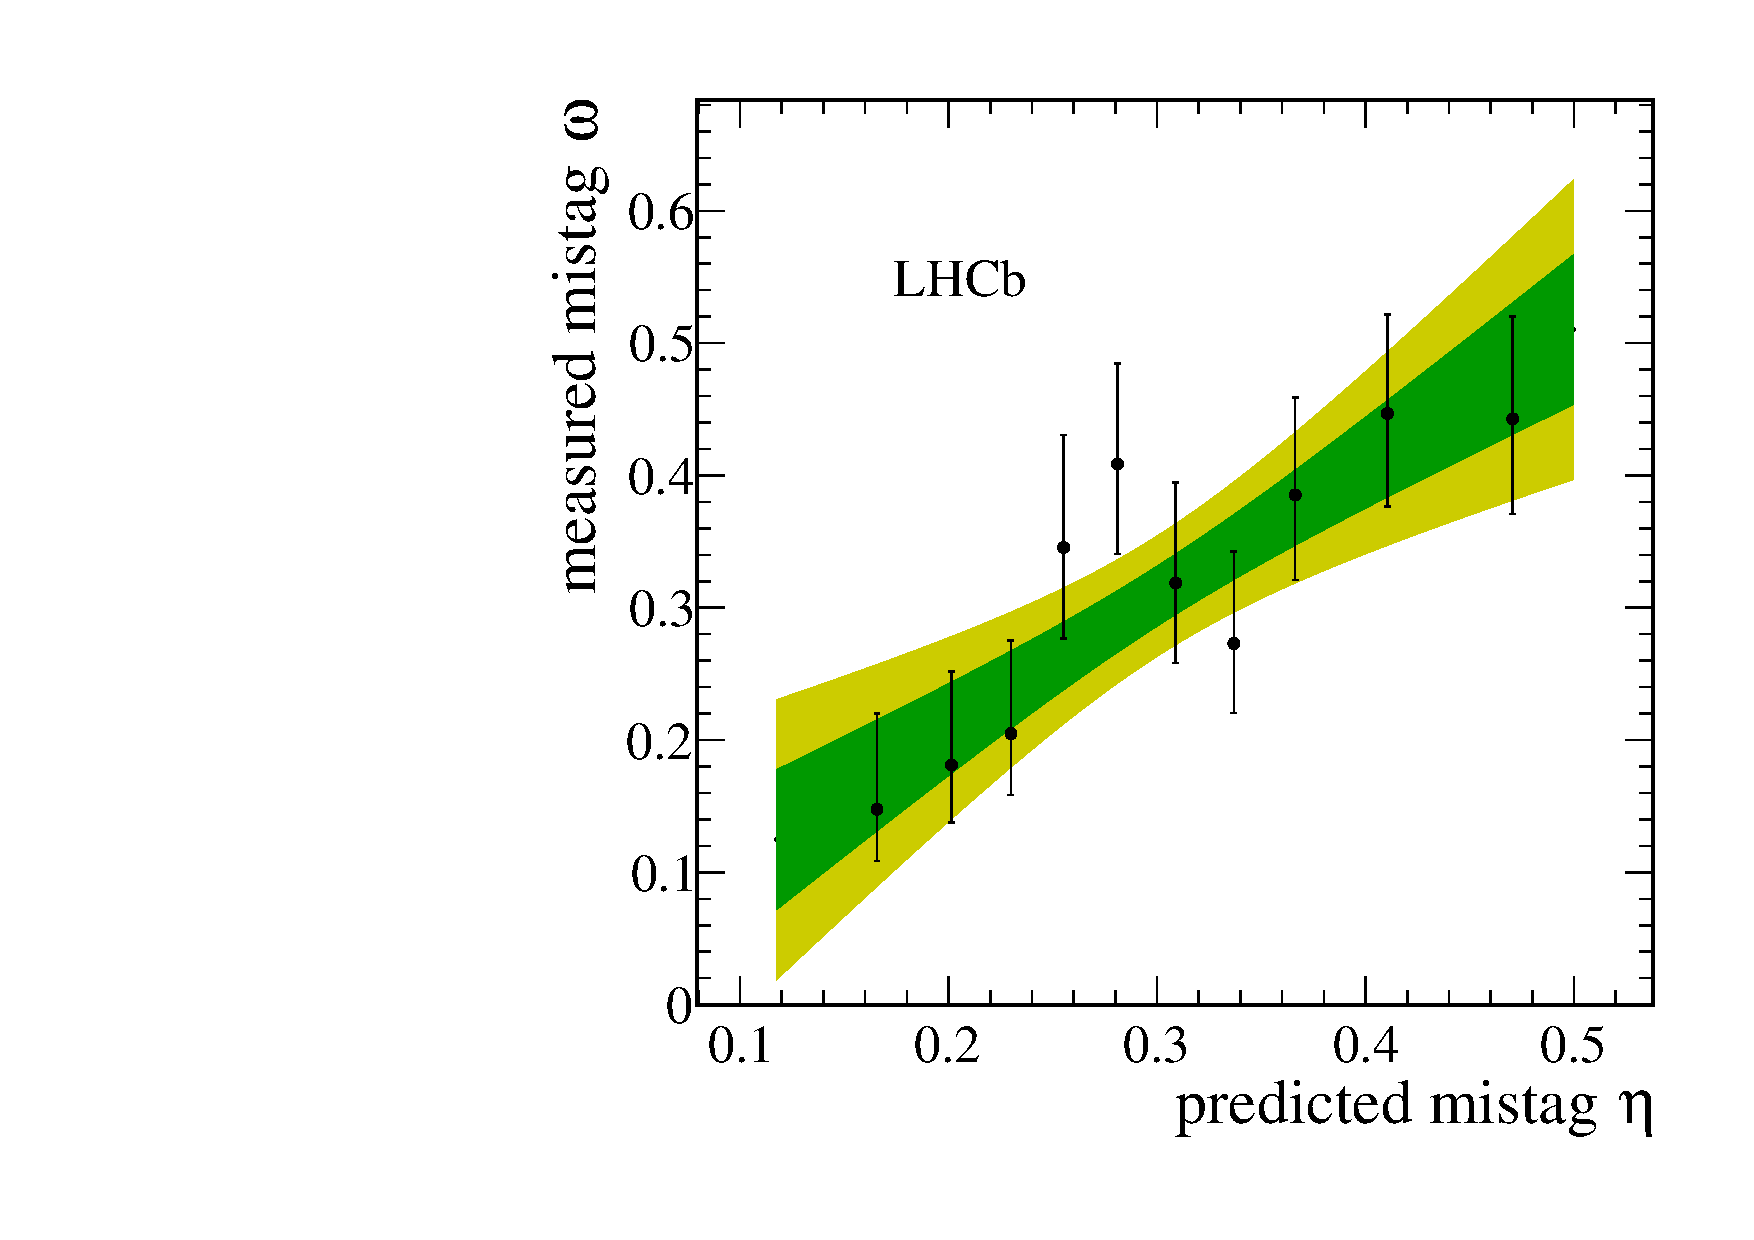
\includegraphics[height=!,width=0.4\textwidth]{figs/Tagging/Run1/OS_Muon_Calibration.pdf}
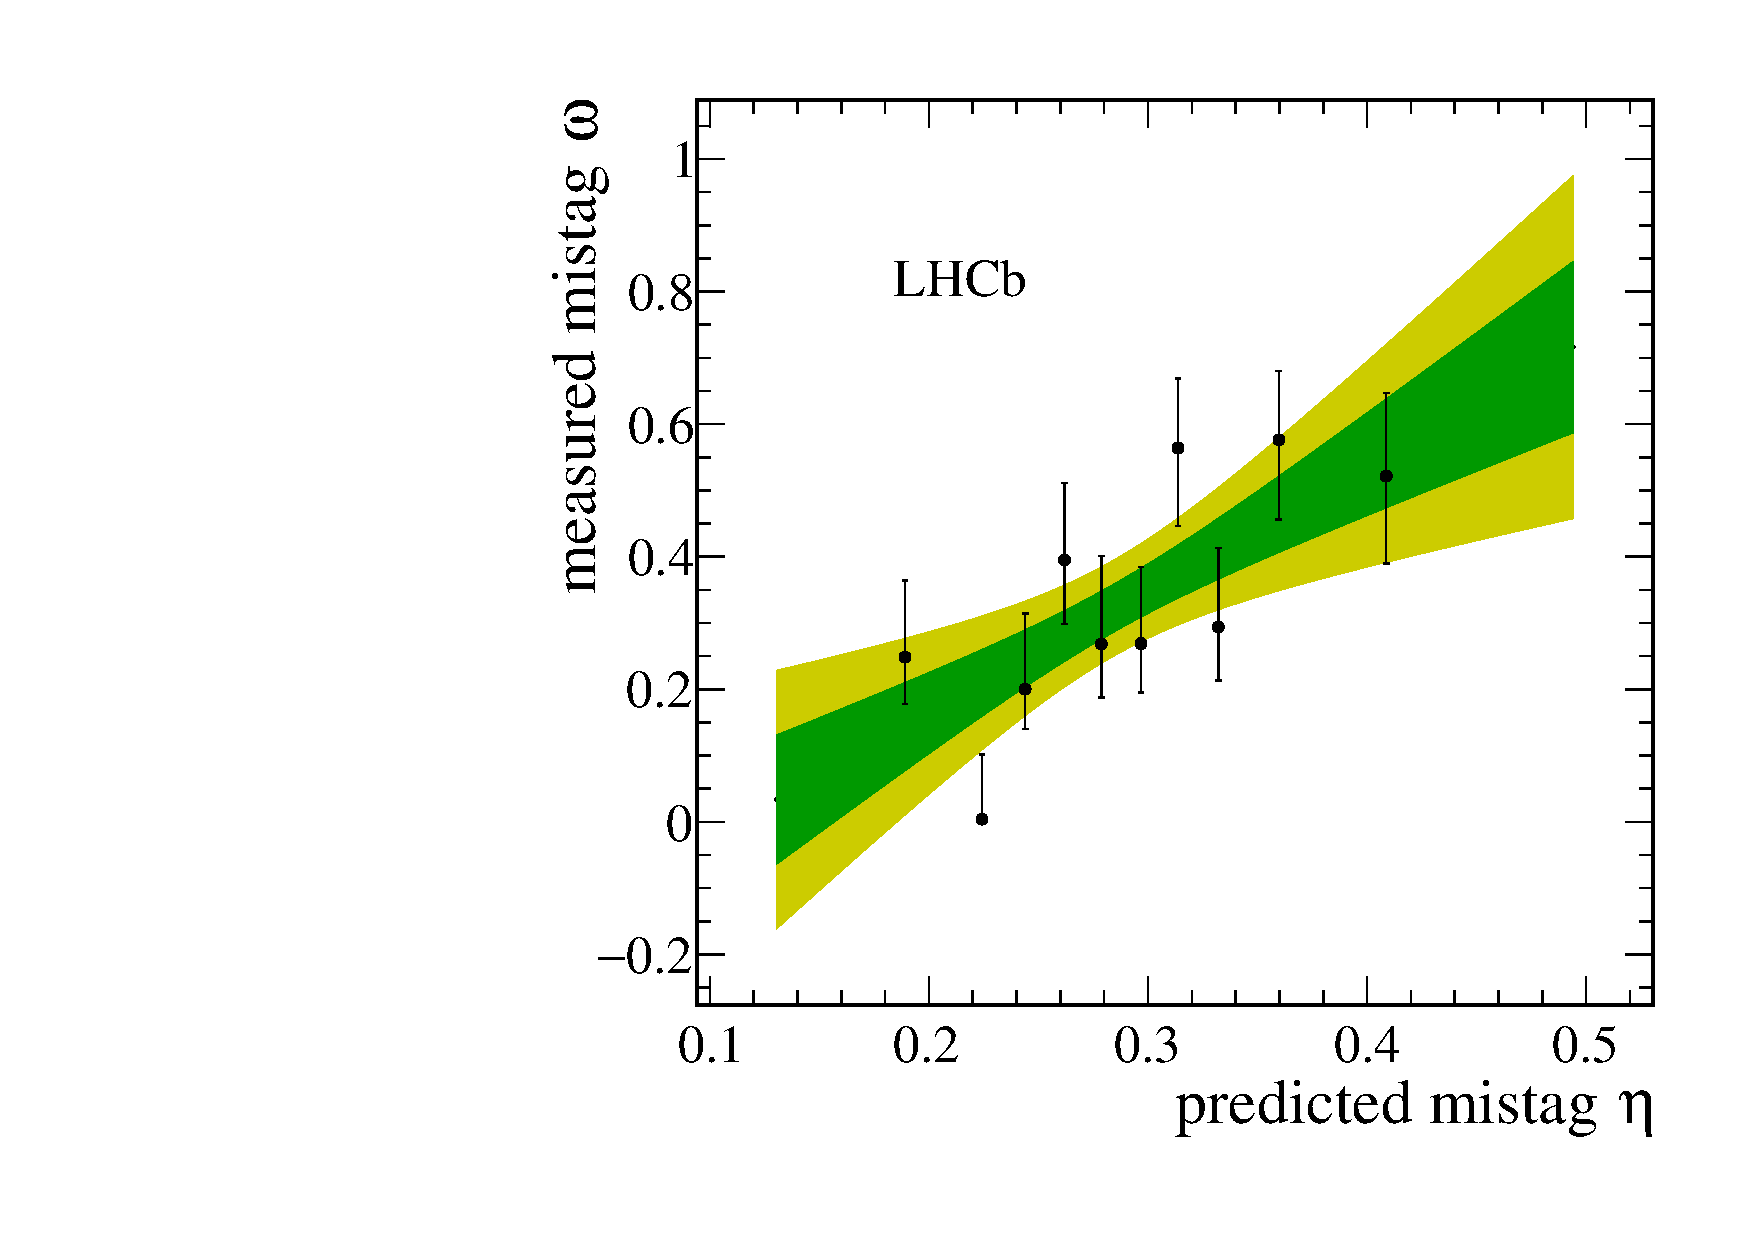
\includegraphics[height=!,width=0.4\textwidth]{figs/Tagging/Run1/OS_Electron_Calibration.pdf}

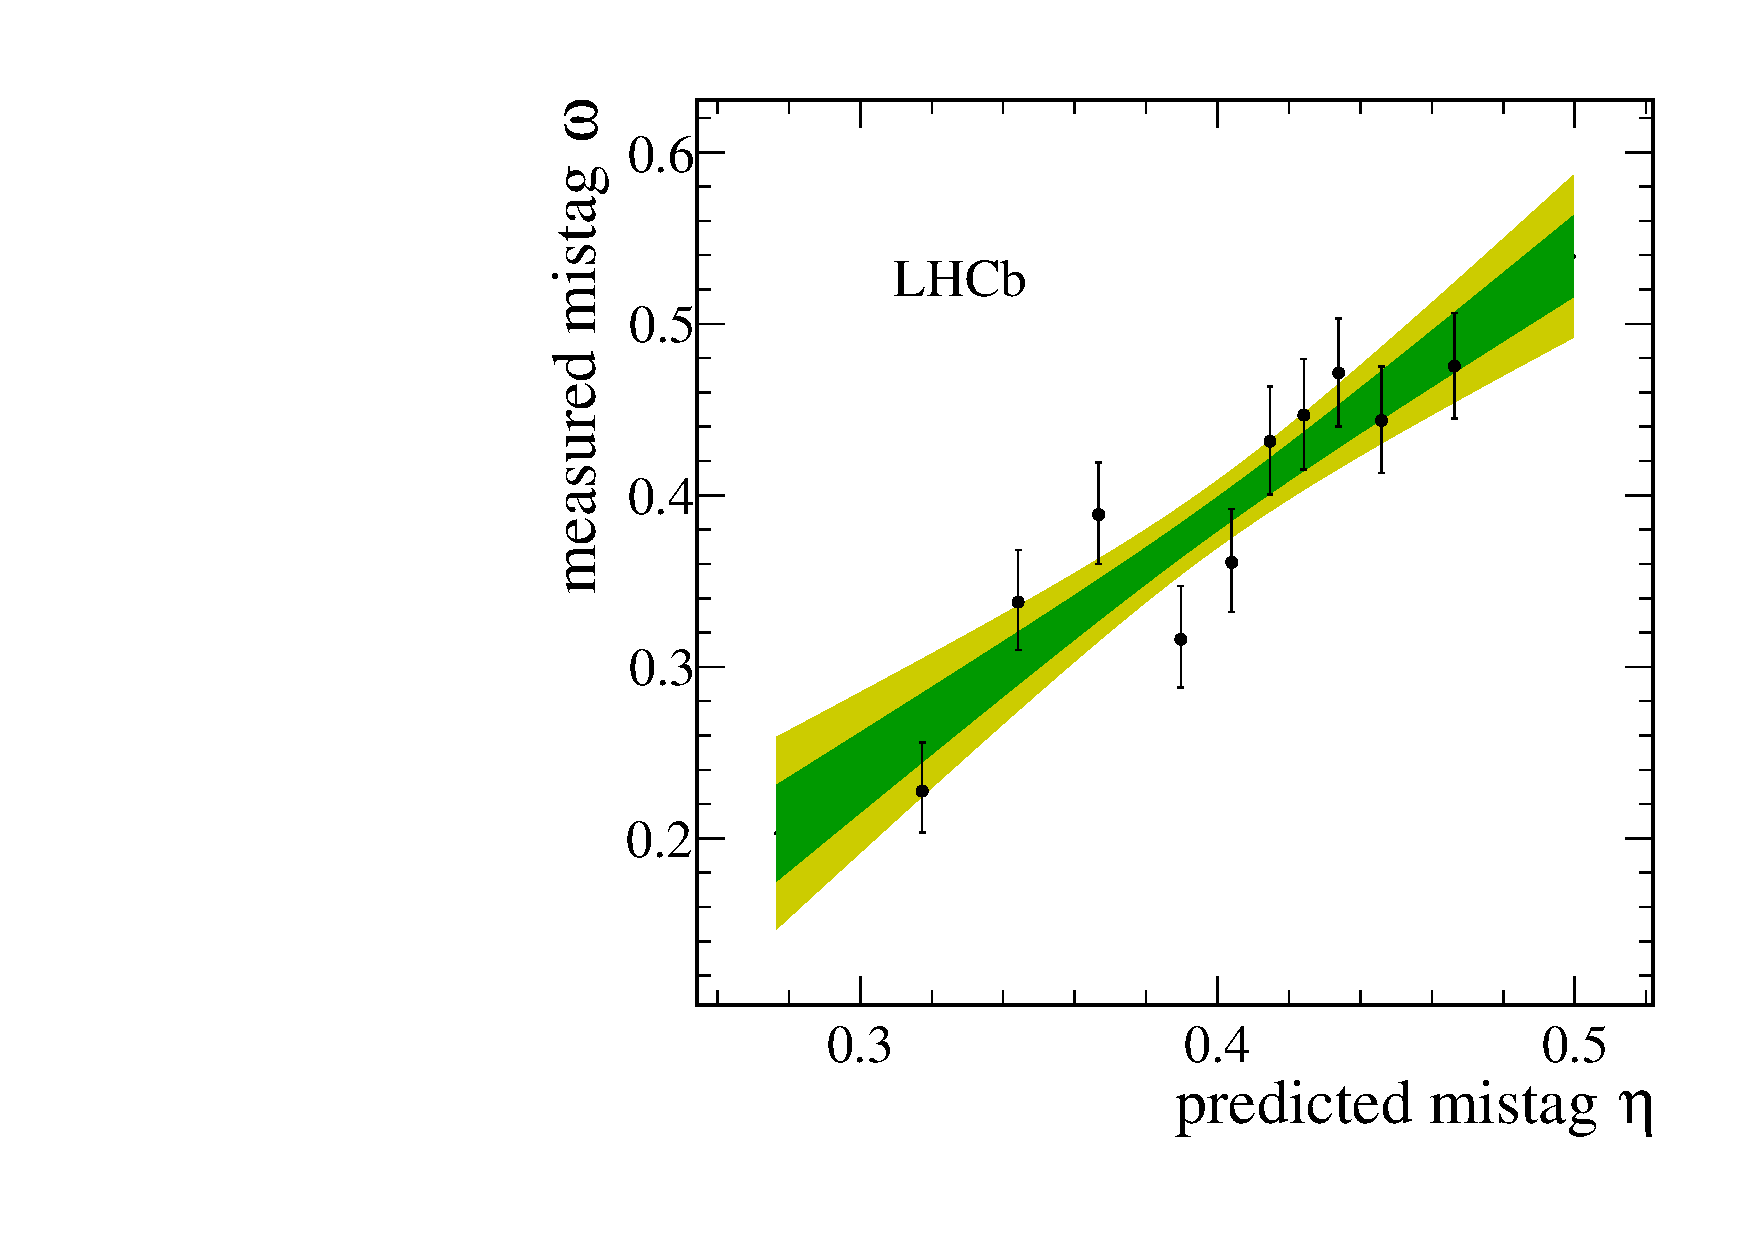
\includegraphics[height=!,width=0.4\textwidth]{figs/Tagging/Run1/OS_nnetKaon_Calibration.pdf}
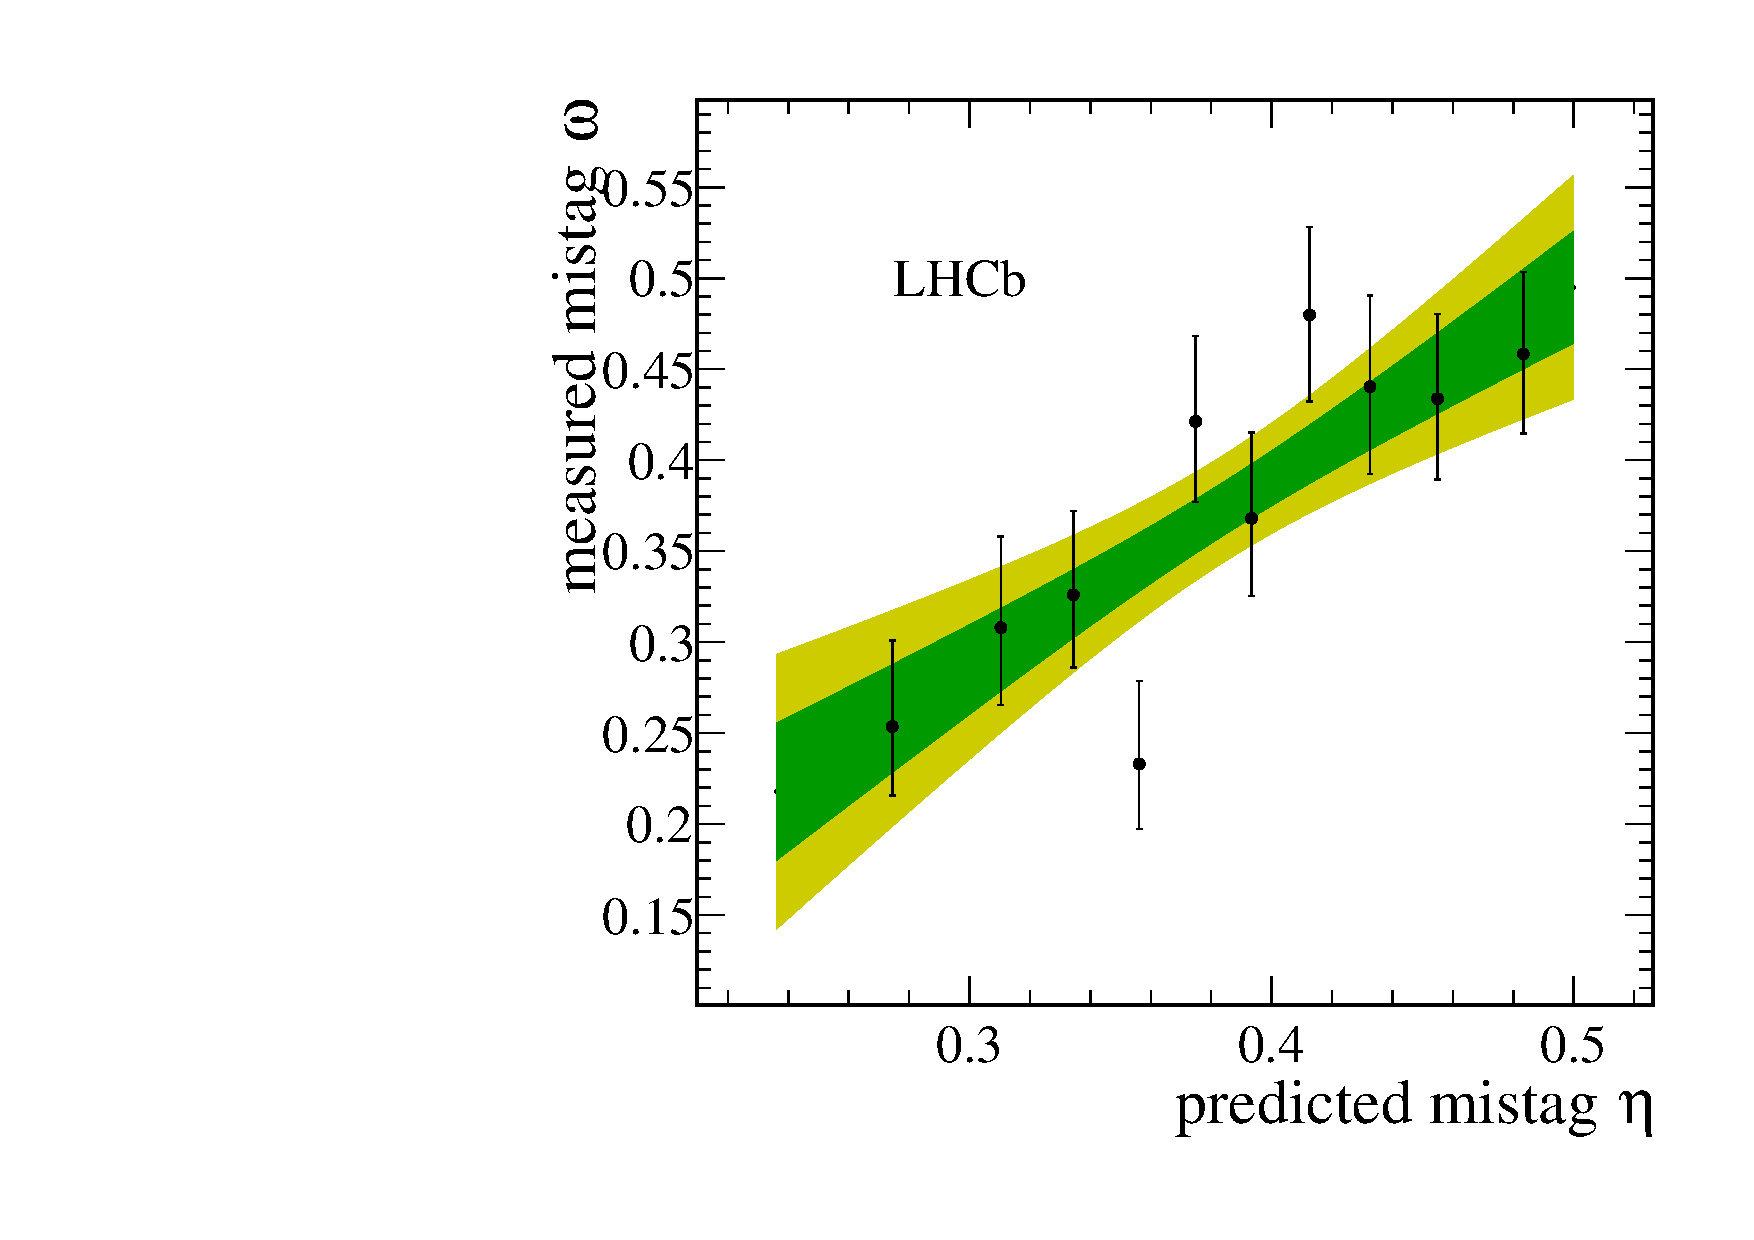
\includegraphics[height=!,width=0.4\textwidth]{figs/Tagging/Run1/VtxCharge_Calibration.pdf}
\caption{}
\label{fig:}
\end{figure}

\begin{figure}[h]
\centering
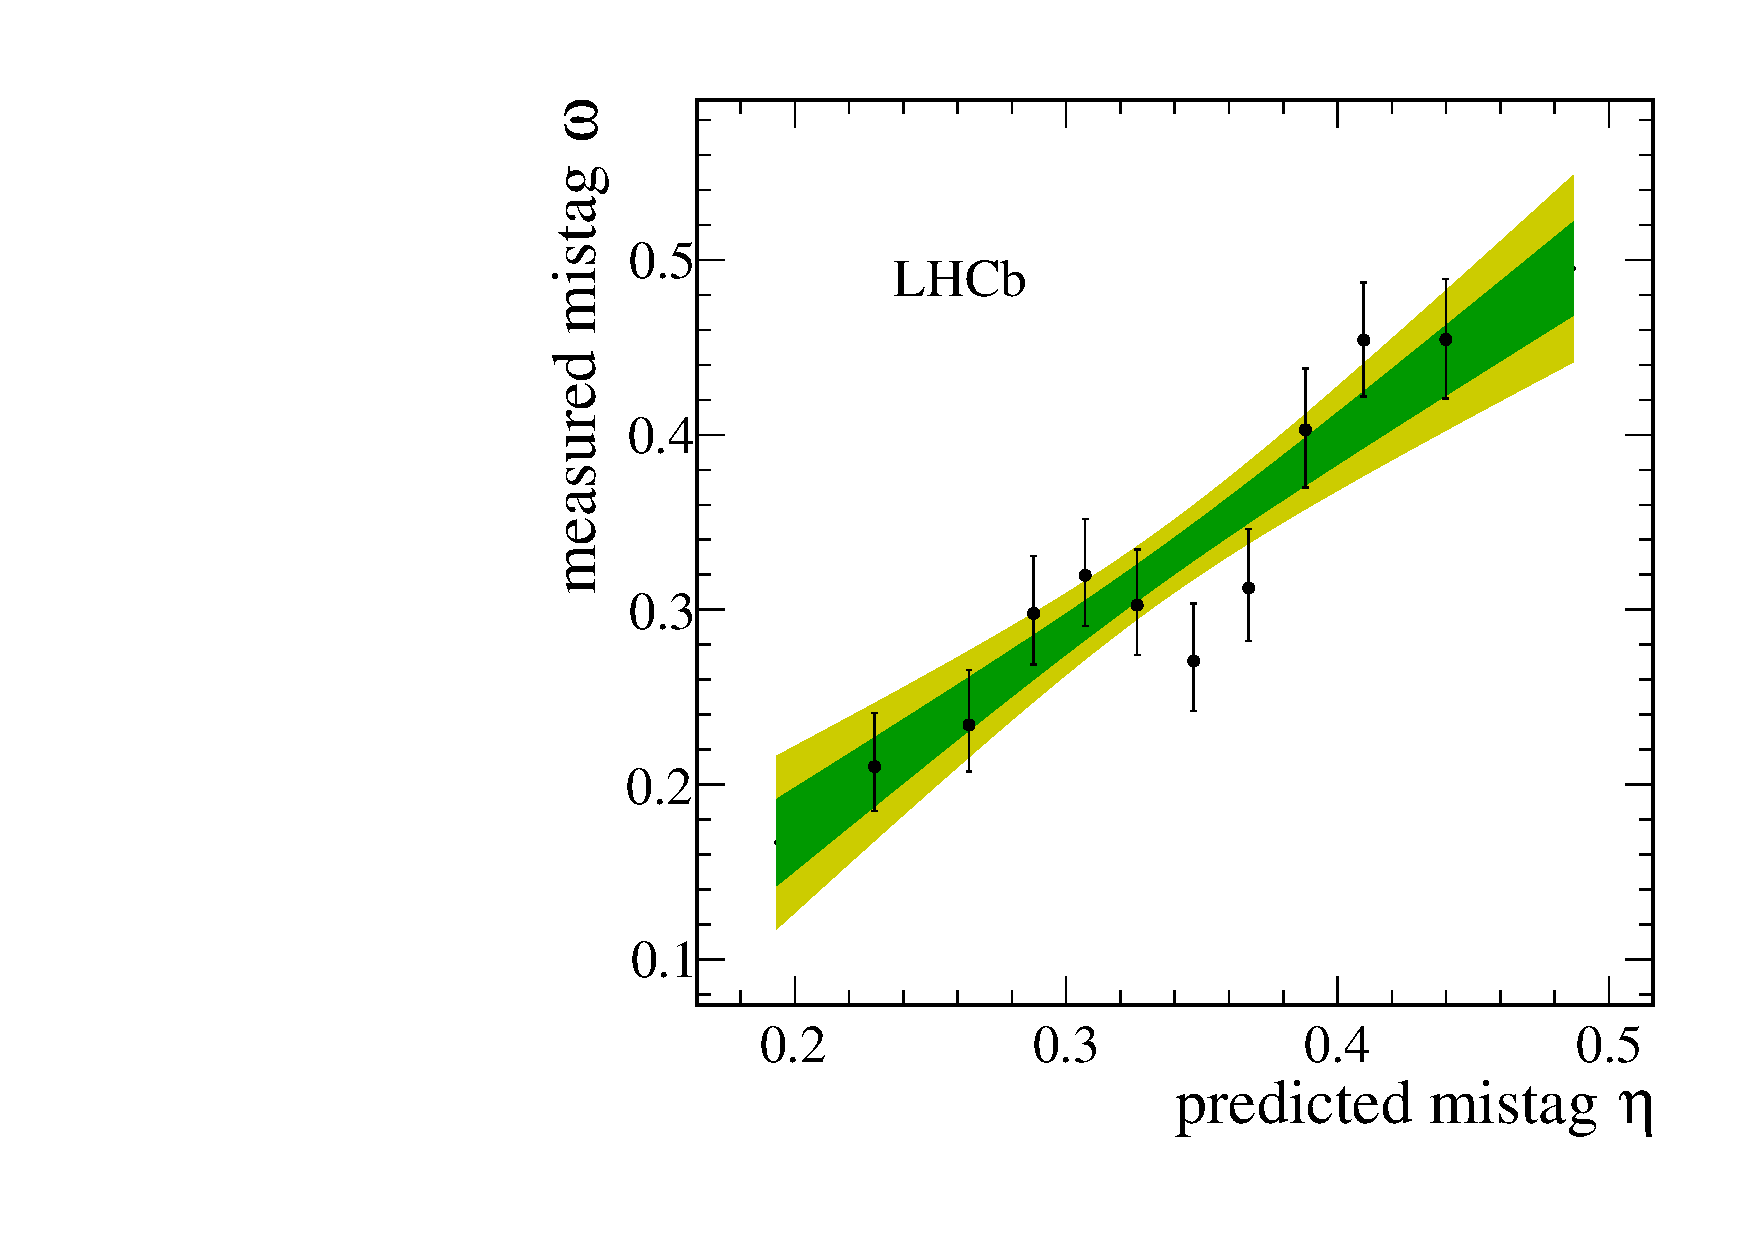
\includegraphics[height=!,width=0.4\textwidth]{figs/Tagging/Run2/OS_Muon_Calibration.pdf}
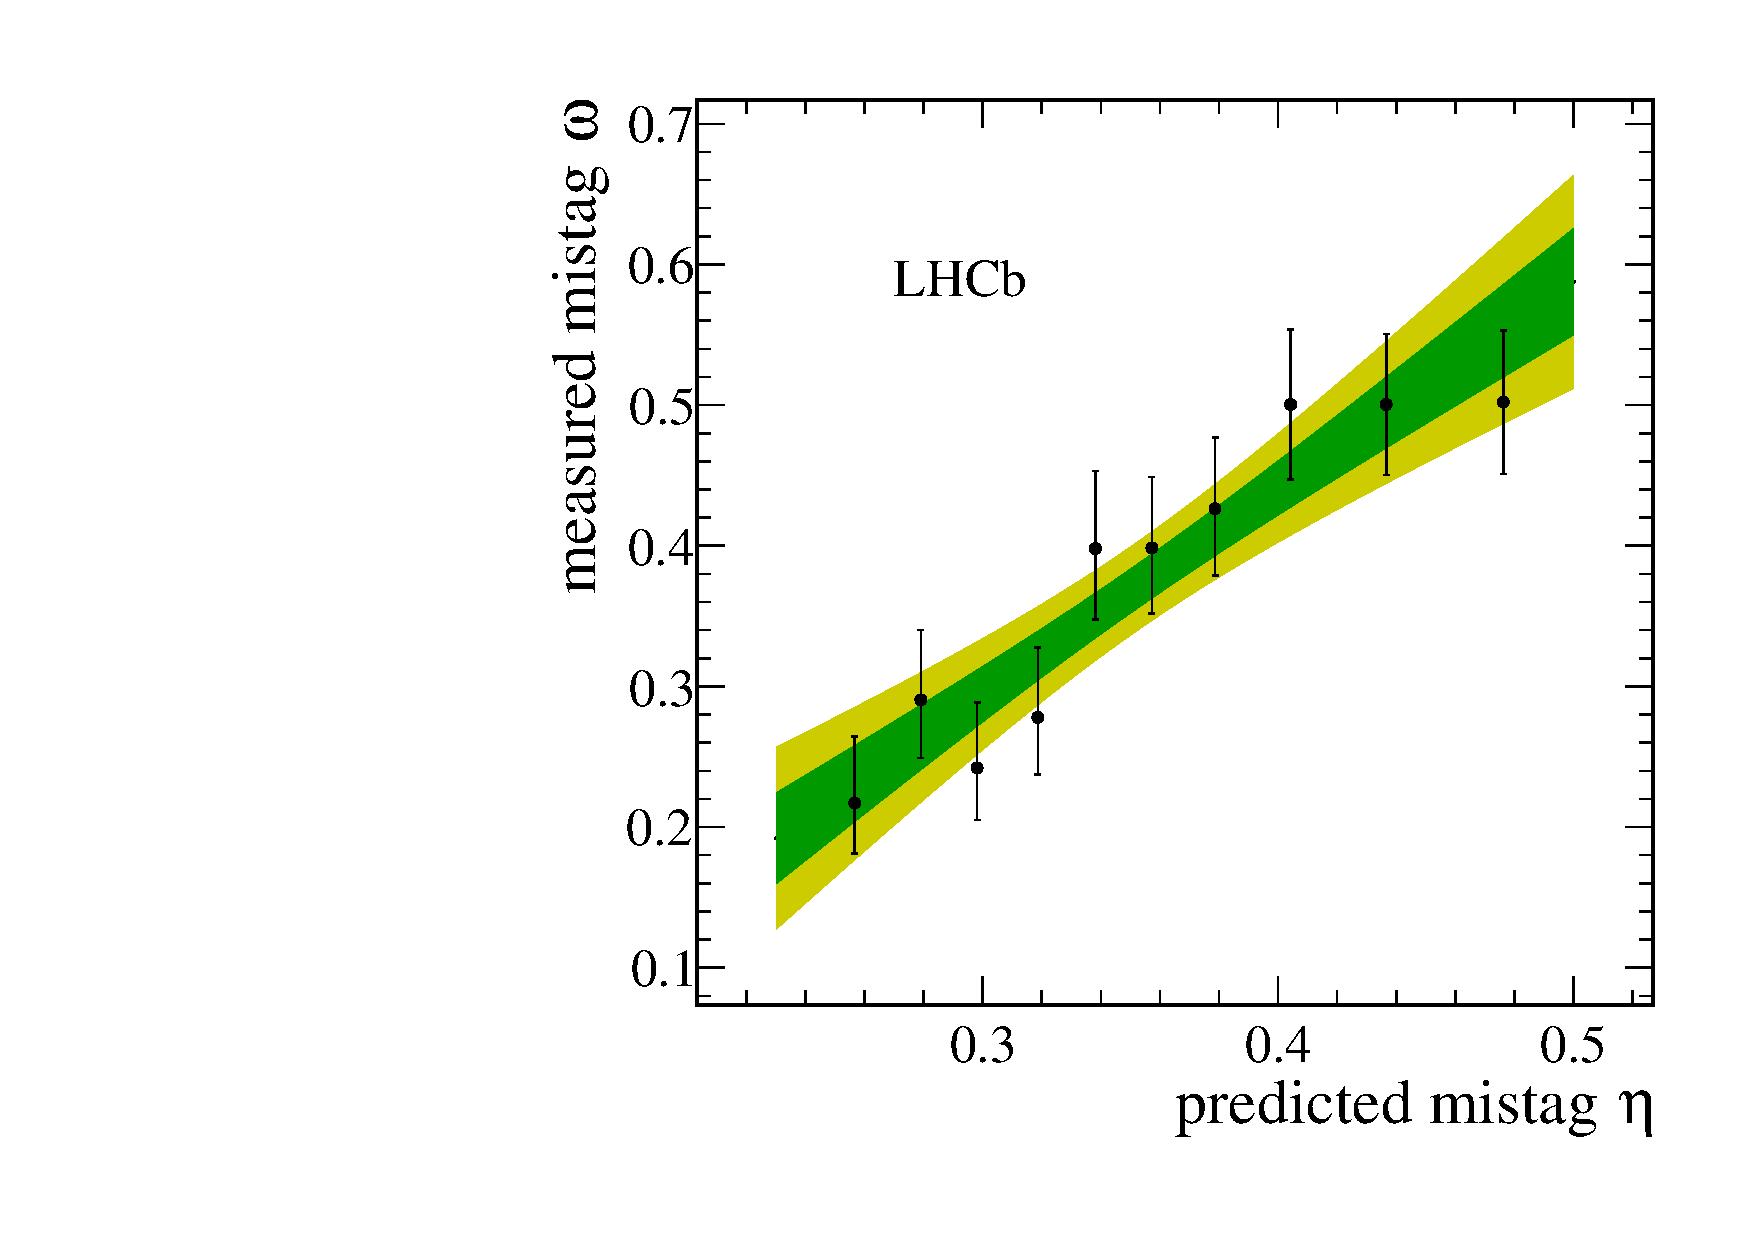
\includegraphics[height=!,width=0.4\textwidth]{figs/Tagging/Run2/OS_Electron_Calibration.pdf}

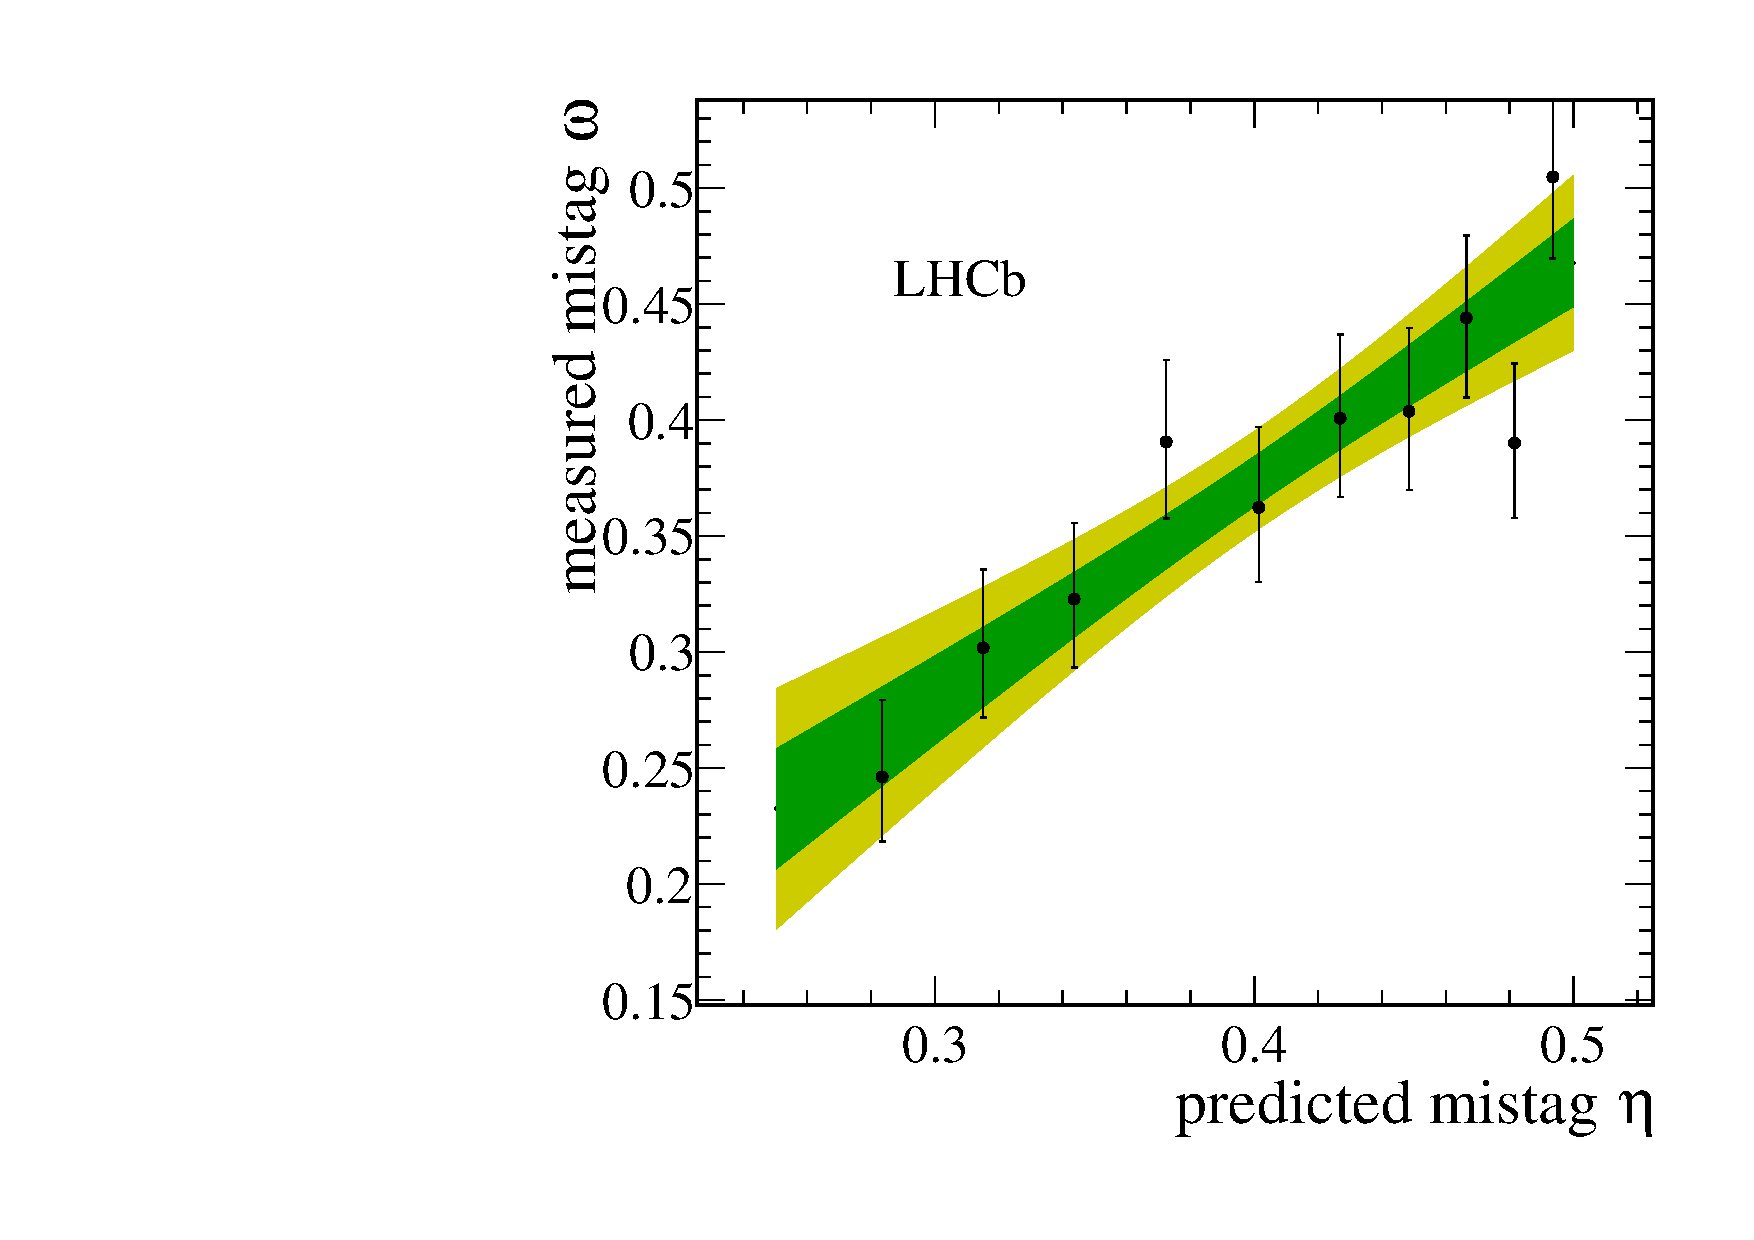
\includegraphics[height=!,width=0.4\textwidth]{figs/Tagging/Run2/OS_nnetKaon_Calibration.pdf}
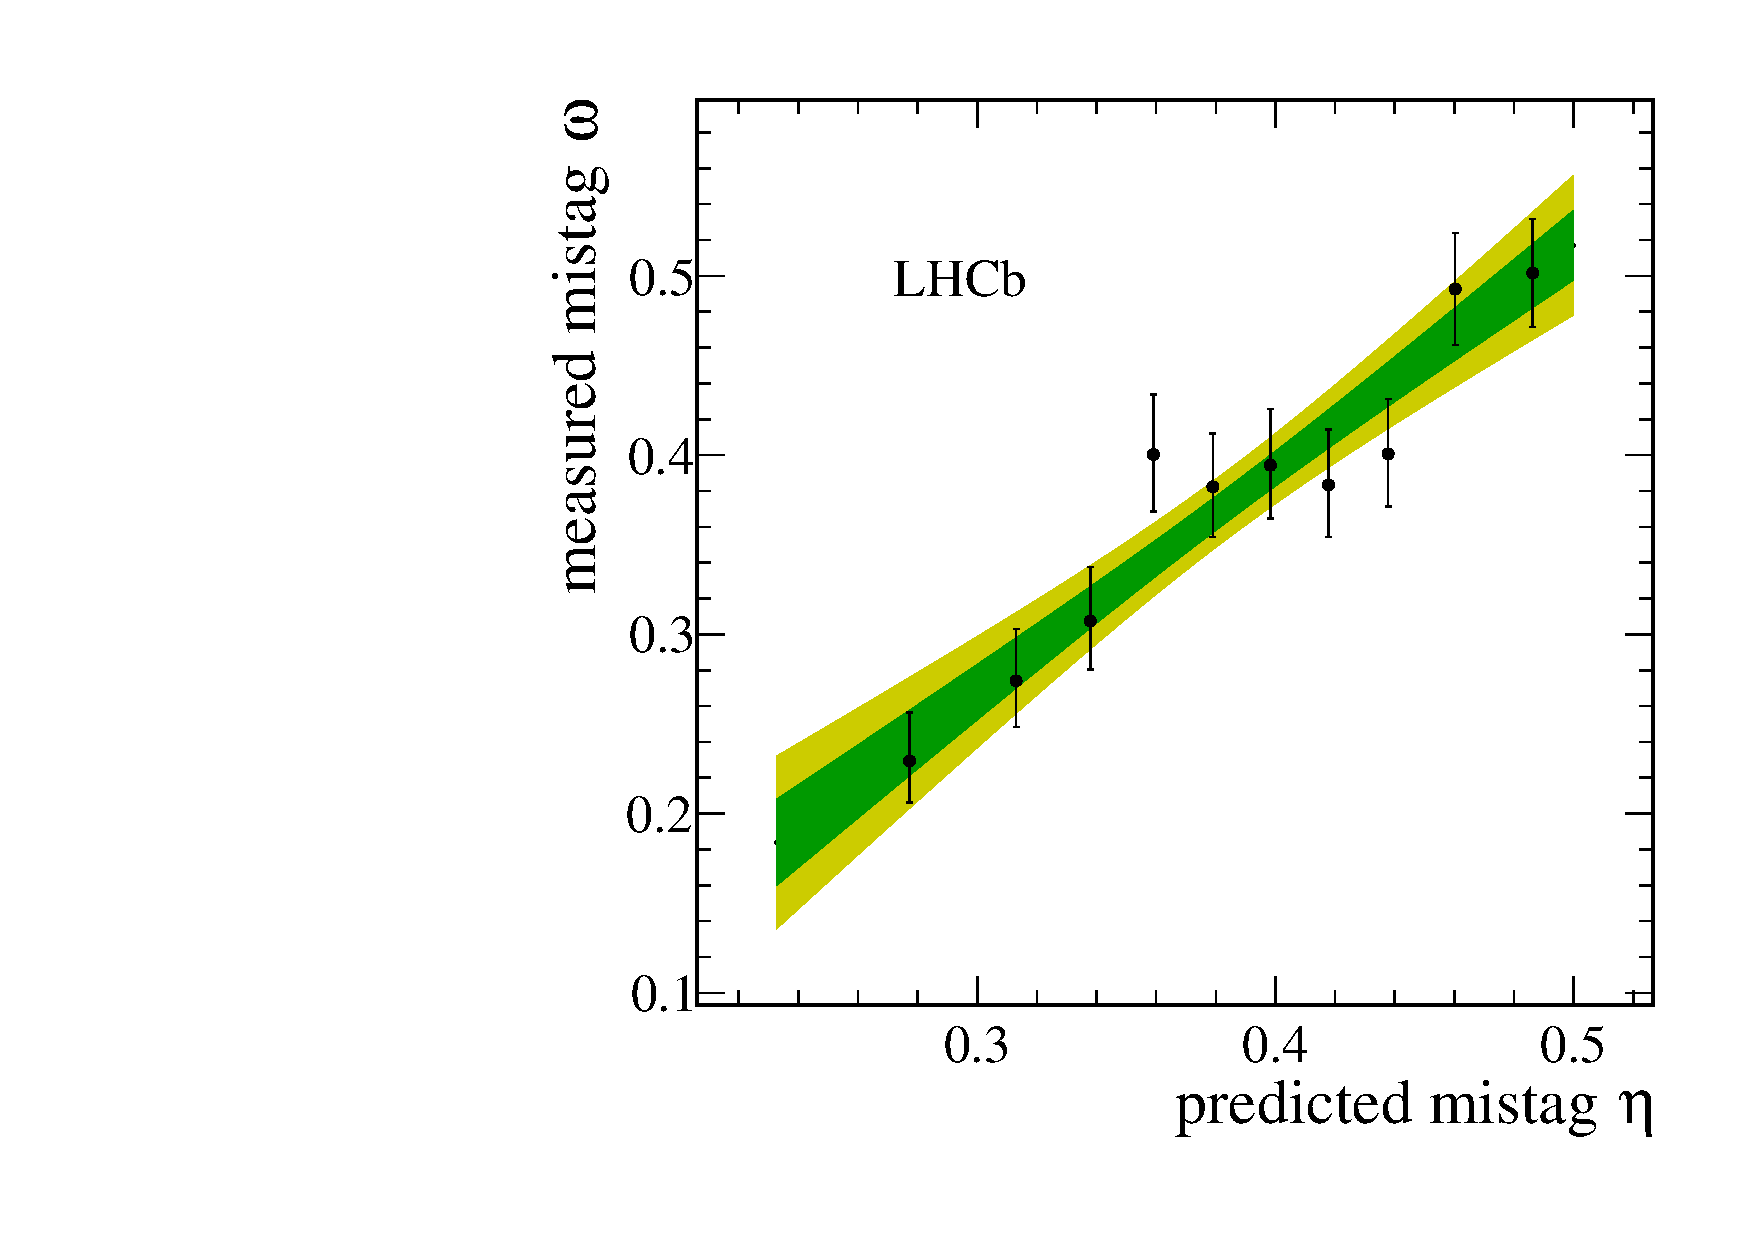
\includegraphics[height=!,width=0.4\textwidth]{figs/Tagging/Run2/VtxCharge_Calibration.pdf}
\caption{}
\label{fig:}
\end{figure}

%\begin{table}
\centering
\begin{tabular}{rlllll}
\multicolumn{1}{c}{Tagger} & \multicolumn{1}{c}{$\epsilon$} & \multicolumn{1}{c}{$\omega$} & \multicolumn{1}{c}{$\epsilon \langle D^2 \rangle = \epsilon \left( 1 - 2 \omega \right)^2$} \\ 
OS $\mu$& $(8.775\pm0.207)\%$& $(28.935\pm0.180(\textrm{stat})\pm2.288(\textrm{cal}))\%$& $(1.558\pm0.045(\textrm{stat})\pm0.338(\textrm{cal}))\%$\\
OS $e$& $(3.191\pm0.129)\%$& $(28.778\pm0.366(\textrm{stat})\pm3.636(\textrm{cal}))\%$& $(0.575\pm0.031(\textrm{stat})\pm0.197(\textrm{cal}))\%$\\
OS $K$ NN& $(32.099\pm0.342)\%$& $(38.405\pm0.094(\textrm{stat})\pm1.152(\textrm{cal}))\%$& $(1.726\pm0.033(\textrm{stat})\pm0.343(\textrm{cal}))\%$\\
Vertex Charge& $(21.797\pm0.302)\%$& $(35.672\pm0.092(\textrm{stat})\pm1.480(\textrm{cal}))\%$& $(1.790\pm0.034(\textrm{stat})\pm0.370(\textrm{cal}))\%$\\
\end{tabular}
\end{table}

%\begin{table}
\centering
\begin{tabular}{rlllll}
\multicolumn{1}{c}{Tagger} & \multicolumn{1}{c}{$\epsilon$} & \multicolumn{1}{c}{$\omega$} & \multicolumn{1}{c}{$\epsilon \langle D^2 \rangle = \epsilon \left( 1 - 2 \omega \right)^2$} \\ 
OS $\mu$& $(8.775\pm0.207)\%$& $(28.935\pm0.180(\textrm{stat})\pm2.288(\textrm{cal}))\%$& $(1.558\pm0.045(\textrm{stat})\pm0.338(\textrm{cal}))\%$\\
OS $e$& $(3.191\pm0.129)\%$& $(28.778\pm0.366(\textrm{stat})\pm3.636(\textrm{cal}))\%$& $(0.575\pm0.031(\textrm{stat})\pm0.197(\textrm{cal}))\%$\\
OS $K$ NN& $(32.099\pm0.342)\%$& $(38.405\pm0.094(\textrm{stat})\pm1.152(\textrm{cal}))\%$& $(1.726\pm0.033(\textrm{stat})\pm0.343(\textrm{cal}))\%$\\
Vertex Charge& $(21.797\pm0.302)\%$& $(35.672\pm0.092(\textrm{stat})\pm1.480(\textrm{cal}))\%$& $(1.790\pm0.034(\textrm{stat})\pm0.370(\textrm{cal}))\%$\\
\end{tabular}
\end{table}



%\begin{table}[h]
%\centering
%\scriptsize
% \begin{tabular}{l l l l | l l | l}
%\hline
%$p_{0}$ & $p_{1}$ & $<\eta>$ & $\epsilon_{tag}$ & $\Delta p_{o}$ & $\Delta p_{1}$ & $\epsilon_{eff}$ [$\%$] \\
%\hline
%0.025 $\pm$0.005  & 0.944 $\pm$ 0.048 & 0.347 & 0.517 $\pm$ 0.002 & 0.028 $\pm$ 0.005 & 0.037 $\pm$ 0.045 & 4.81 $\pm$ 0.04 (stat) $\pm$ 0.37 (cal) \\
%\hline
%\end{tabular}
%\caption{Calibration parameters and tagging asymmetries of the OS tagger extracted from $\Bs\to\Ds\pion\pion\pion$ decays.}
%\label{table: OScalibration}
%\normalsize
%\end{table}


\subsection{SS tagging calibration}
\label{subsec: SScalibration}
The SS neural net kaon tagger can be calibrated using the flavour-specific $\Bs\to\Ds\pion\pion\pion$ decay. It's development, performance and calibration is described in detail in \cite{Aaij:2016psi}. 
Figure \ref{fig:SSdistribution} shows the distribution of the predicted mistag of the neural net kaon tagger. 
The extracted calibration parameters and tagging asymmetries are summarized in Table \ref{table: SScalibration} and the measured tagging power for this algorithm is $\epsilon_{eff,SS} = 3.22  \%$.

\begin{table}[h]
\centering
\scriptsize
 \begin{tabular}{l l l l | l l | l}
\hline
$p_{0}$ & $p_{1}$ & $<\eta>$ & $\epsilon_{tag}$ & $\Delta p_{o}$ & $\Delta p_{1}$ & $\epsilon_{eff}$ [$\%$] \\
\hline
0.008 $\pm$ 0.004  & 1.086 $\pm$ 0.059 & 0.381 & 0.571 $\pm$ 0.002 & -0.017 $\pm$ 0.004  & 0.135 $\pm$ 0.058 & 3.22 $\pm$ 0.03 (stat) $\pm$ 0.26 (cal) \\
\hline
\end{tabular}
\caption{Calibration parameters and tagging asymmetries of the SS tagger extracted from $\Bs\to\Ds\pion\pion\pion$ decays.}
\label{table: SScalibration}
\normalsize
\end{table}


\subsection{Tagging performance comparison between the signal and normalization channel}
\label{subsec: TaggingComparison}

To justify the usage of the tagging calibration, obtained using the $\Bs\to\Ds\pion\pion\pion$ sample, for our signal decay, the performance of the taggers in the two decay channels needs to be compatible. 
This is verified using both, simulated signal samples of both decays and sweighted data, 
to compare the similarity of the mistag probabilities, tagging decisions and kinematic observables that are correlated with the tagging response, on simulation and data.  \newline
The distributions of the predicted mistag probability $\eta$ for the OS combination and the SS kaon tagger are shown in Fig. \ref{fig:w_MC_comparison} (simulation) and Fig. \ref{fig:w_data_comparison} (data).
 

%\begin{figure}[h]
%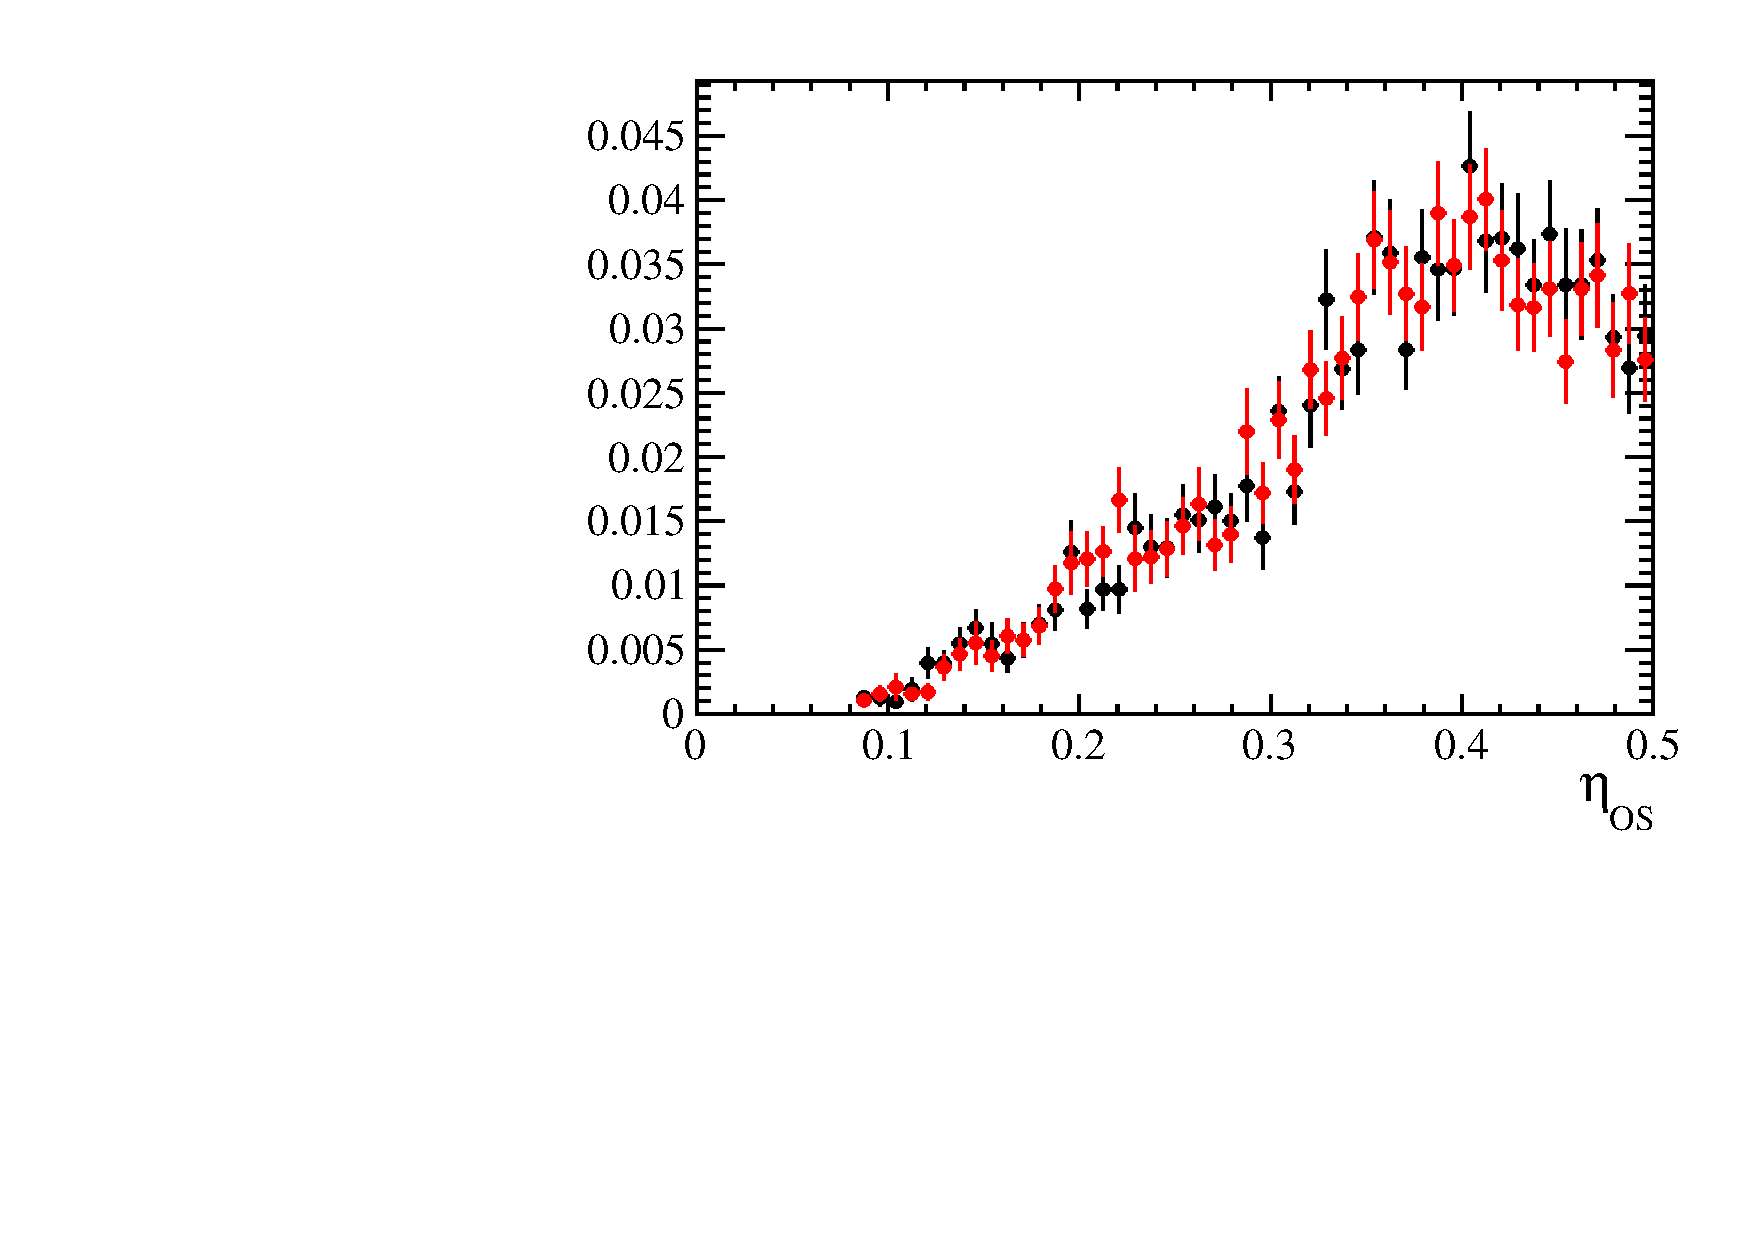
\includegraphics[height=7.cm,width=0.49\textwidth]{figs/Tagging/w_OS_MC.pdf}
%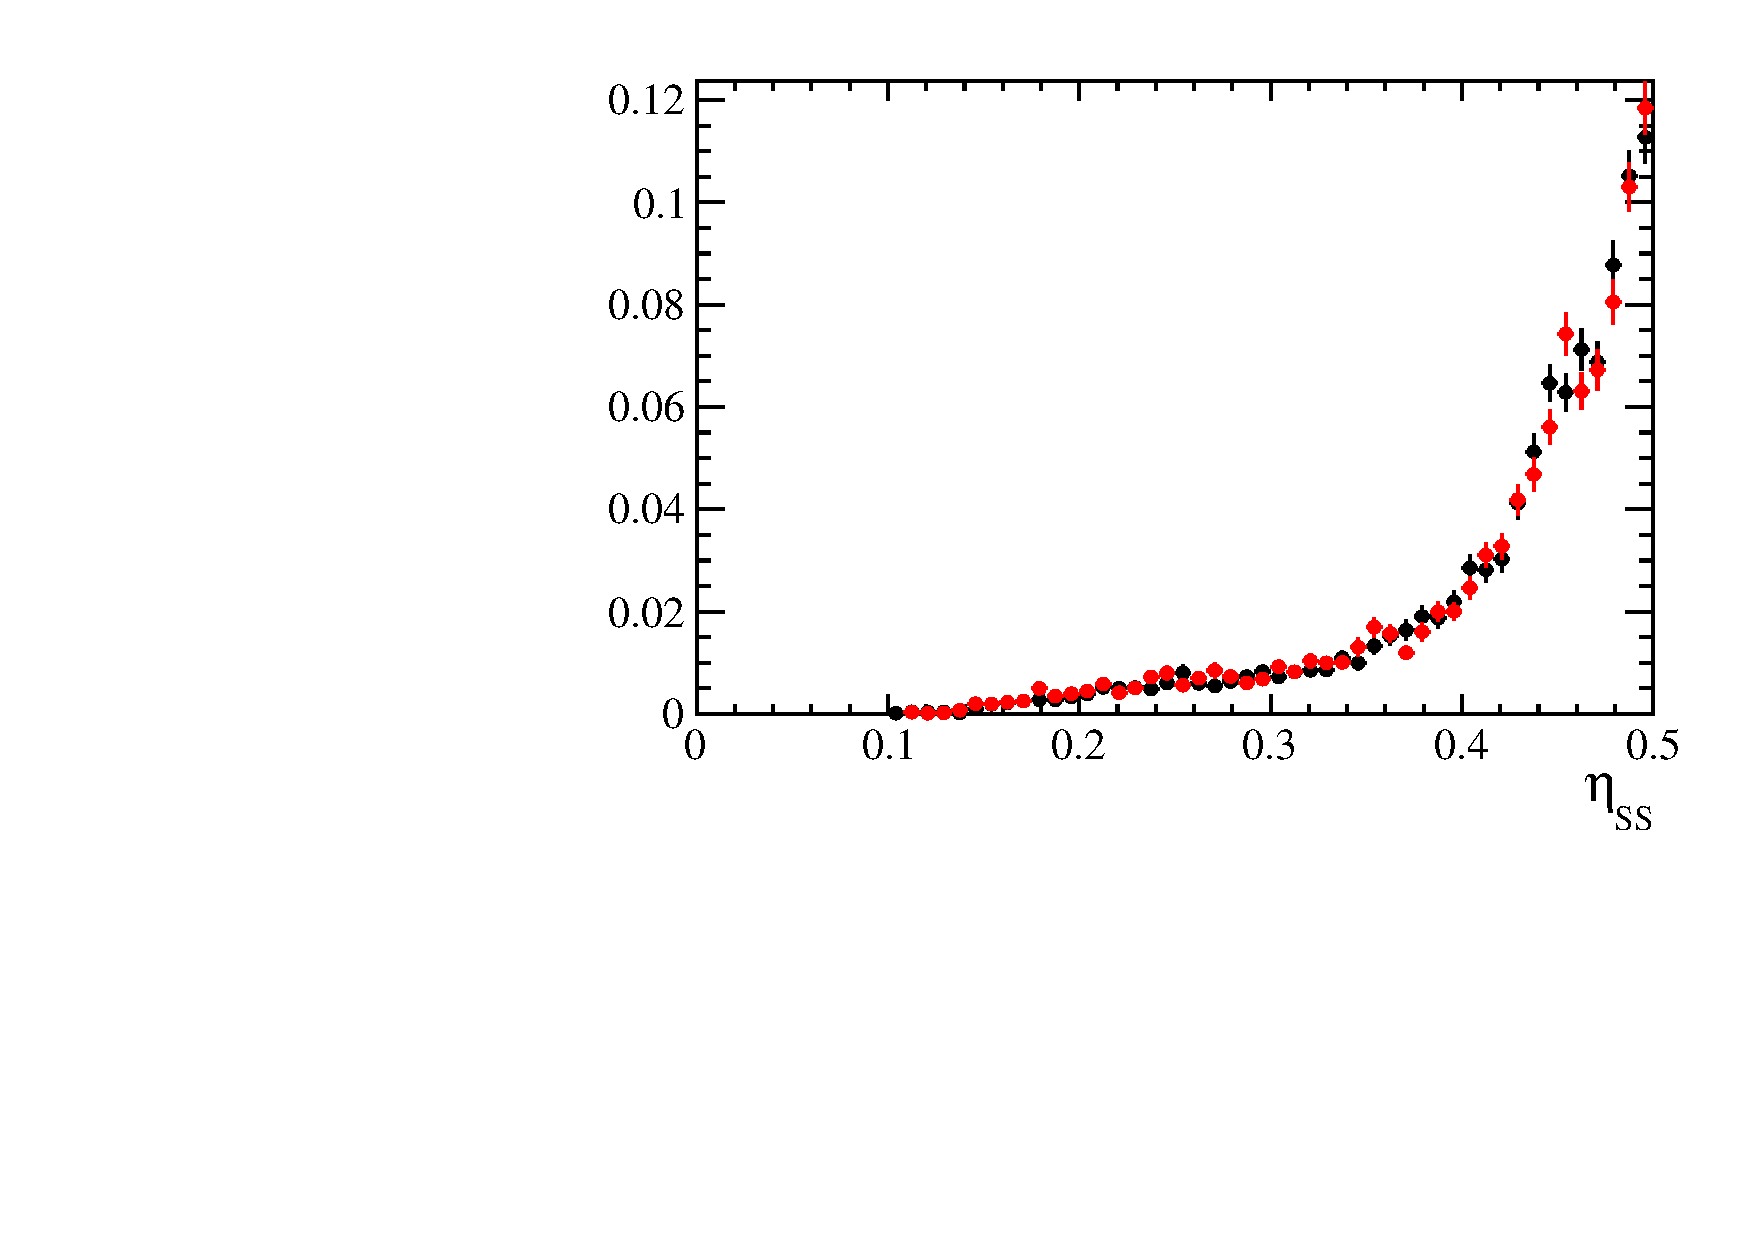
\includegraphics[height=7.cm,width=0.49\textwidth]{figs/Tagging/w_SS_MC.pdf}
%\caption{Distributions of the predicted mistag $\eta$ for the OS combination (left) and the SS kaon tagger (right) in simulated $\Bs\to\Ds\kaon\pion\pion$ (black) and $\Bs\to\Ds\pion\pion\pion$ (red) signal.}
%\label{fig:w_MC_comparison}
%\end{figure}

\begin{figure}[h]
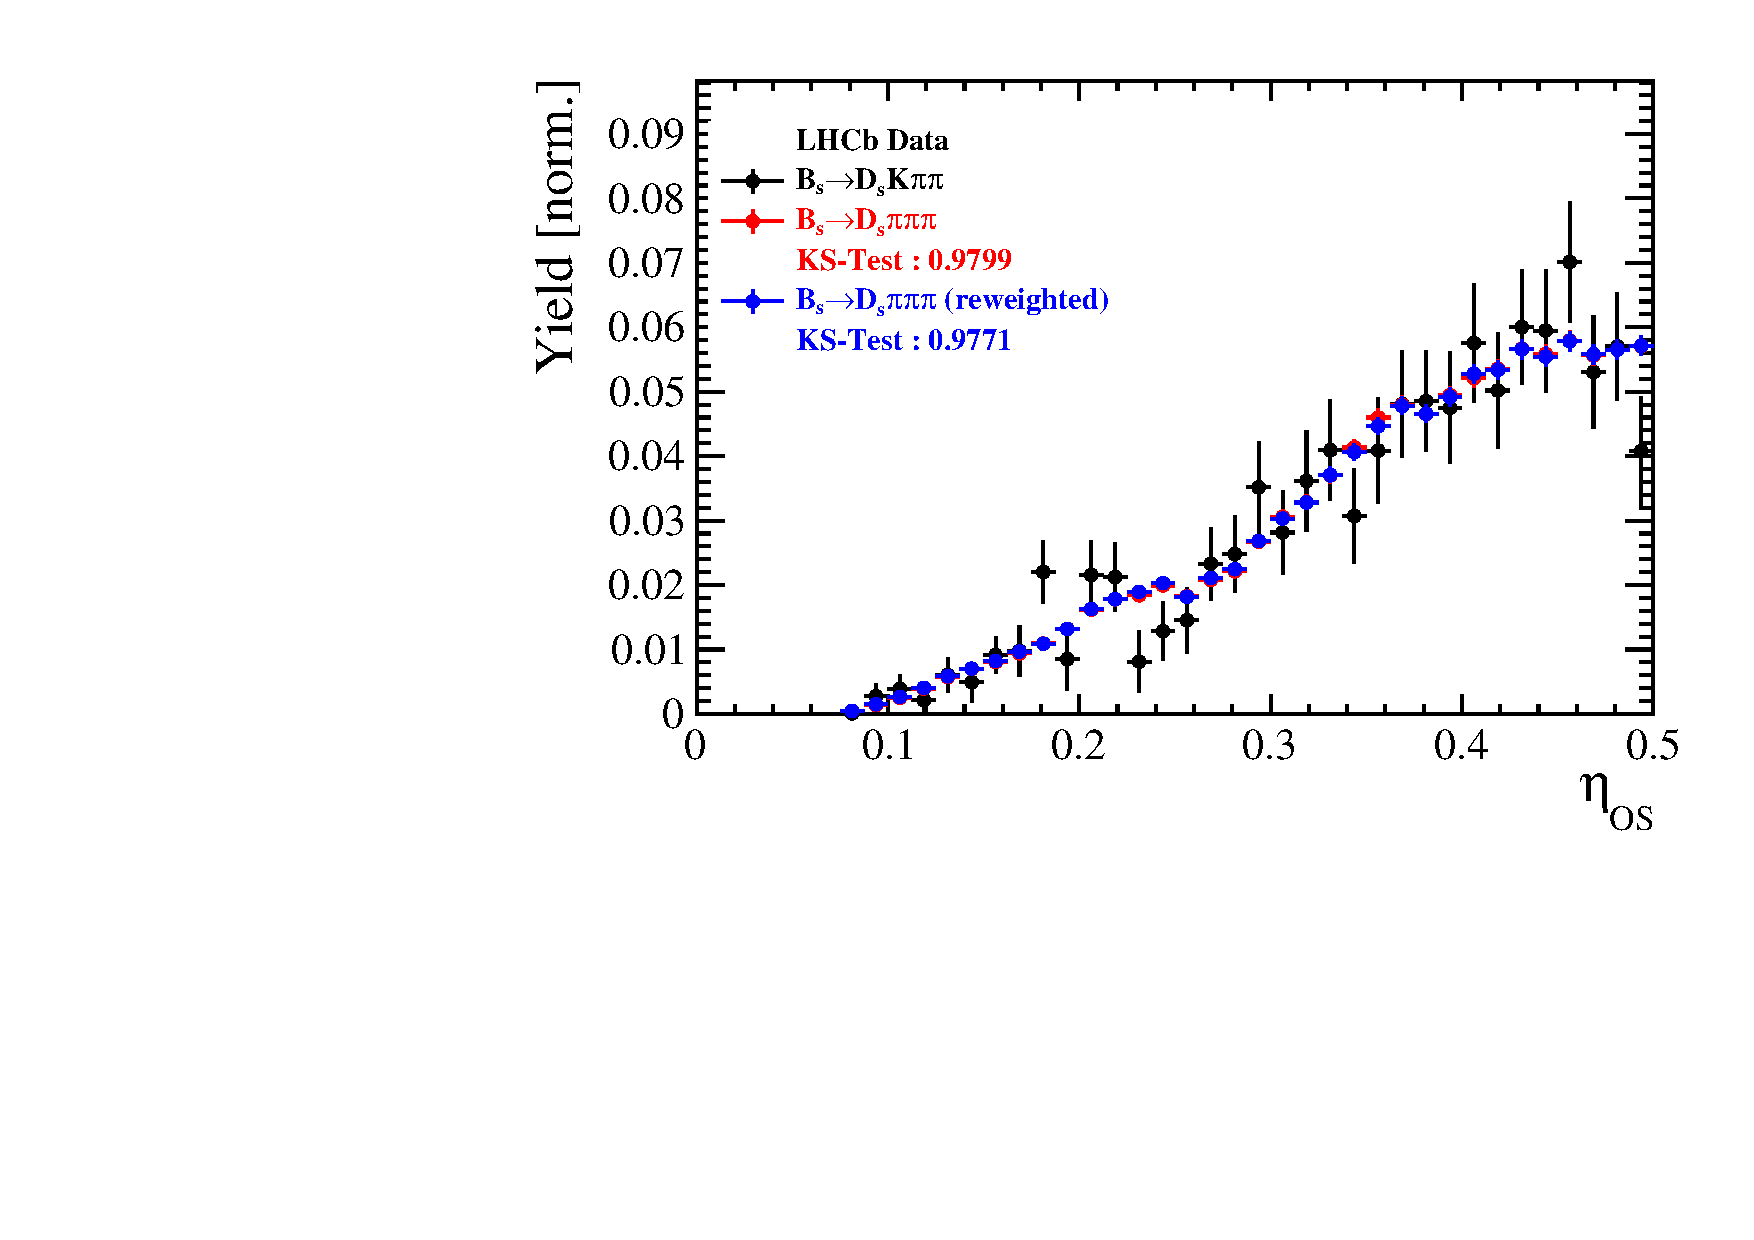
\includegraphics[height=!,width=0.5\textwidth]{figs/dataVsMC/norm2signal/Ds2all_Bs_TAGOMEGA_OS.pdf}
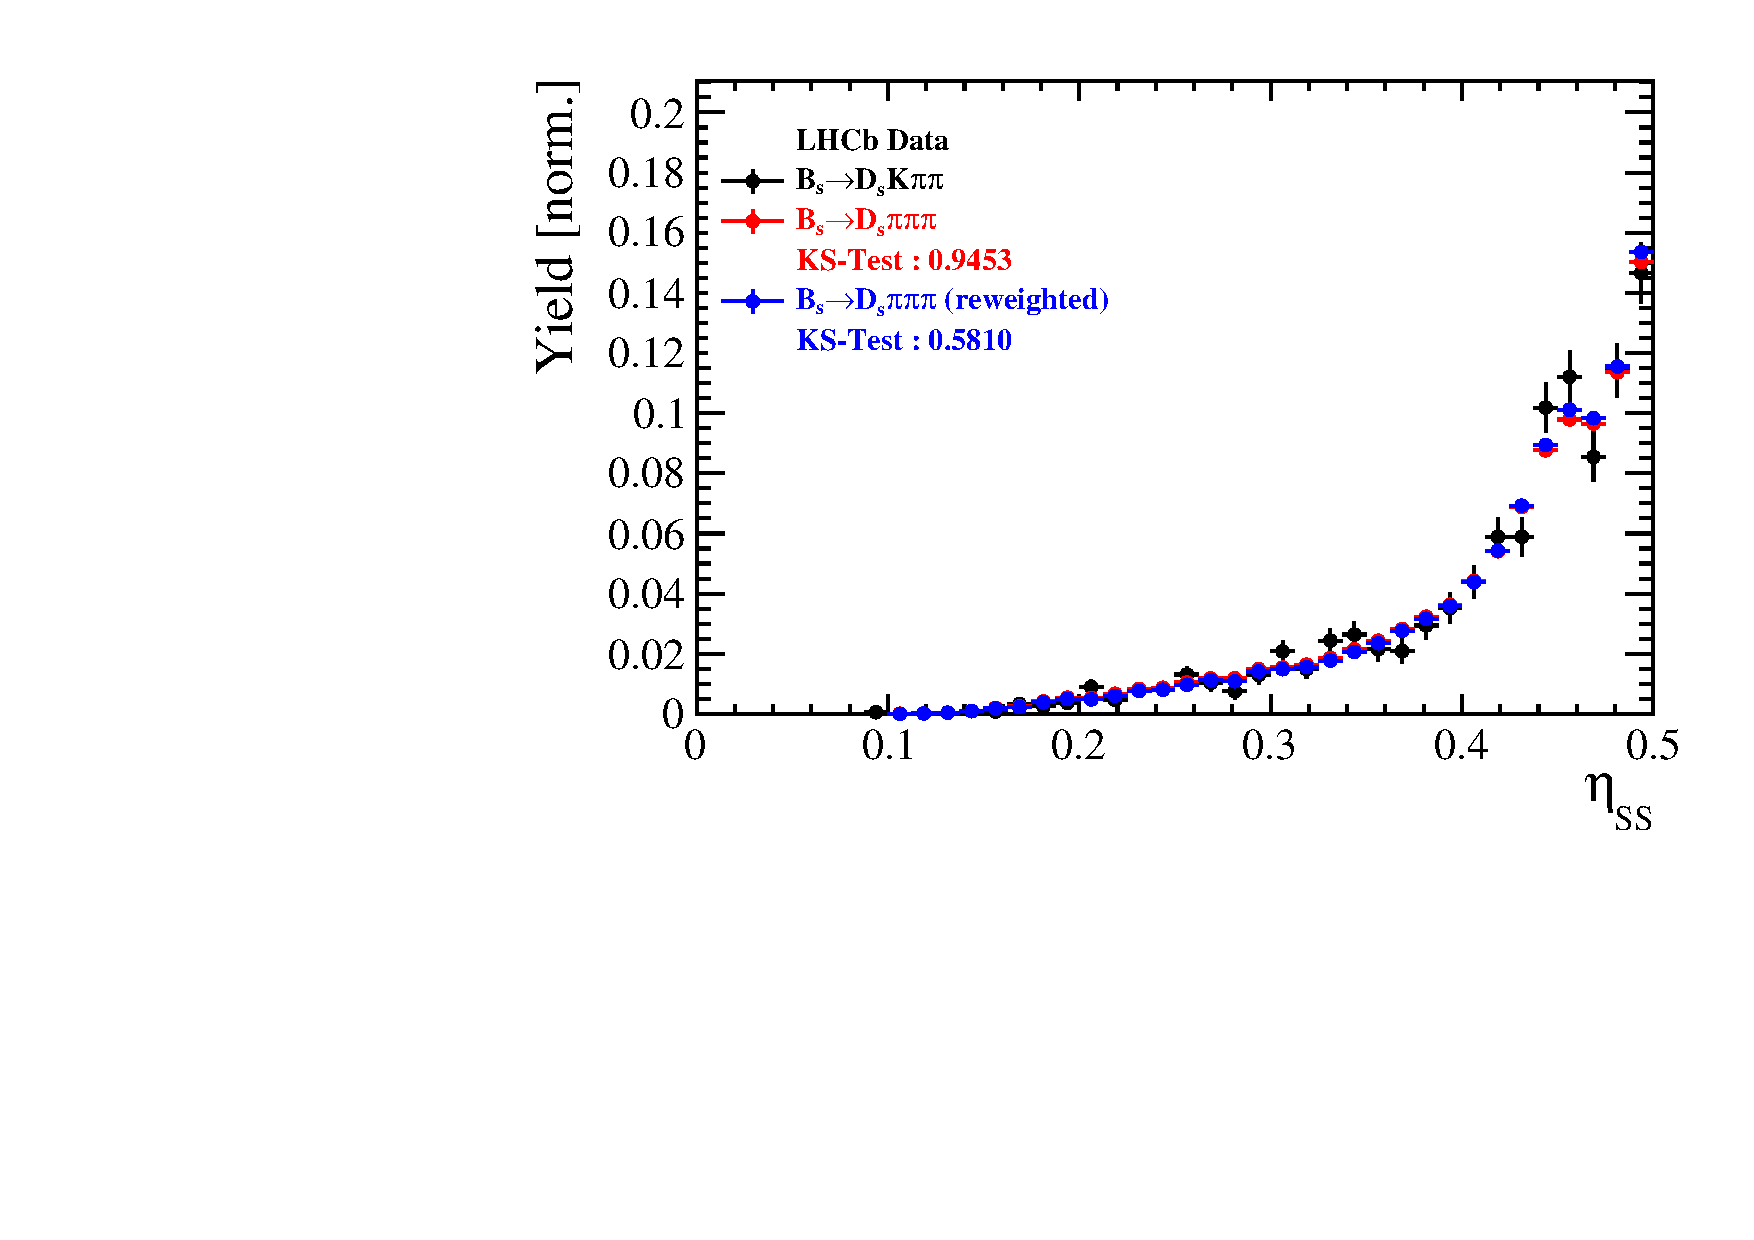
\includegraphics[height=!,width=0.5\textwidth]{figs/dataVsMC/norm2signal/Ds2all_Bs_SS_nnetKaon_PROB.pdf}
\caption{Distributions of the predicted mistag $\eta$ for the OS combination (left) and the SS kaon tagger (right) 
for signal candidates in the $\Bs\to\Ds\kaon\pion\pion$ (black) and $\Bs\to\Ds\pion\pion\pion$ (red) data samples.}
\label{fig:w_data_comparison}
\end{figure}

Both, data and simulated samples, show good agreement between the signal and normalization channel. 
Compatibility is also seen in Fig. \ref{fig:tagDec_data_comparison}, which shows the comparison of the tagging decision distributions of the OS and SS tagger for sweighted data. 

%\begin{figure}[h]
%\includegraphics[height=7.cm,width=0.49\textwidth]{figs/Tagging/qOS.pdf}
%\includegraphics[height=7.cm,width=0.49\textwidth]{figs/Tagging/q_SS.pdf}
%\caption{Distributions of the tagging decision from the OS combination (left) and the SS kaon tagger (right) for signal candidates in the $\Bs\to\Ds\kaon\pion\pion$ (black) and $\Bs\to\Ds\pion\pion\pion$ (red) data samples. 
%The signal distributions are obtained using sWeights, the procedure is described in Sec. \ref{subsec: sWegihts}.}
%\label{fig:tagDec_data_comparison}
%\end{figure}


%\begin{figure}[h]
%\includegraphics[height=7.cm,width=0.49\textwidth]{figs/Tagging/OS_Combination_DEC_norm_RunsComparison.pdf}
%\includegraphics[height=7.cm,width=0.49\textwidth]{figs/Tagging/SS_nnetKaon_DEC_norm_RunsComparison.pdf}\\
%\includegraphics[height=7.cm,width=0.49\textwidth]{figs/Tagging/OS_Combination_PROB_norm_RunsComparison.pdf}
%\includegraphics[height=7.cm,width=0.49\textwidth]{figs/Tagging/SS_nnetKaon_PROB_norm_RunsComparison.pdf}
%\caption{Distributions of the tagging decision from the OS combination (upper left) and the SS kaon tagger (upper right), 
%as well as the predicted mistag $\eta$ for OS (bottm left) and the SS  (bottom right), for $\Bs\to\Ds\pion\pion\pion$ candidates in the Run 1 (blue) and Run 2 (green) data samples. 
%The signal distributions are obtained using sWeights, the procedure is described in Sec. \ref{subsec: sWegihts}.}
%\label{fig:kinematics_data_comparison}
%\end{figure}

Fig. \ref{fig:kinematics_data_comparison} shows the signal data distributions of the transverse $\Bs$ momentum $\pt$, the pseudorapidity $\eta$ of the signal candidate and the number of reconstructed tracks per event.
Sufficient agreement is observed.

%\begin{figure}[h]
%\includegraphics[height=7.cm,width=0.49\textwidth]{figs/Tagging/Bs_Pt_comparison.pdf}
%\includegraphics[height=7.cm,width=0.49\textwidth]{figs/Tagging/Bs_eta_comparison.pdf}\\
%\includegraphics[height=7.cm,width=0.49\textwidth]{figs/Tagging/nTracks_comparison.pdf}
%\caption{Distributions of the transverse momentum $\pt$ (top left), 
%the pseudorapidity $\eta$ (top right) and the reconstructed number of tracks in the event (bottom left) for signal candidates in the $\Bs\to\Ds\kaon\pion\pion$ (black) and $\Bs\to\Ds\pion\pion\pion$ (red) data samples. 
%The signal distributions are obtained using sWeights, the procedure is described in Sec. \ref{subsec: sWegihts}.}
%\label{fig:kinematics_data_comparison}
%\end{figure}

%\begin{figure}[h]
%\includegraphics[height=7.cm,width=0.49\textwidth]{figs/Tagging/Bs_Pt_norm_RunsComparison.pdf}
%\includegraphics[height=7.cm,width=0.49\textwidth]{figs/Tagging/Bs_eta_norm_RunsComparison.pdf}\\
%\includegraphics[height=7.cm,width=0.49\textwidth]{figs/Tagging/nTracks_norm_RunsComparison.pdf}
%\caption{Distributions of the transverse momentum $\pt$ (top left), 
%the pseudorapidity $\eta$ (top right) and the reconstructed number of tracks in the event (bottom left) for  $\Bs\to\Ds\pion\pion\pion$ candidates in the Run 1 (blue) and Run 2 (green) data samples. 
%The signal distributions are obtained using sWeights, the procedure is described in Sec. \ref{subsec: sWegihts}.}
%\label{fig:kinematics_data_comparison}
%\end{figure}

To justify the portability of the flavour tagging calibration obtained from $\Bs\to\Ds\pion\pion\pion$ to the $\Bs\to\Ds\kaon\pion\pion$ channel, 
besides the good agreement of the distributions shown above, the dependence of the measured mistag $\omega$ on the predicted mistag $\eta$ has to be compatible in both channel.
This dependence is shown in Fig. \ref{fig:etavsW_mc_comparison} for simulated signal events of both channels, where good agreement is observed. 

\begin{figure}[h]
\includegraphics[height=7.cm,width=0.49\textwidth]{figs/Tagging/OS_combination_MCcomparison.pdf}
\includegraphics[height=7.cm,width=0.49\textwidth]{figs/Tagging/SS_nnetKaon_MCcomparison.pdf}
\caption{Dependence of the observed mistag $\omega$ on the predicted mistag $\eta$ for the (left) OS combination and ther (right) SS kaon tagger, 
found in the simulated $\Bs\to\Ds\kaon\pion\pion$ (black) and $\Bs\to\Ds\pion\pion\pion$ (red) signal samples.}
\label{fig:etavsW_mc_comparison}
\end{figure}


\subsection{Combination of OS and SS taggers}
\label{subsec: TaggingCombination}

In the time- and ampitude-dependent fit to $\Bs\to\Ds\kaon\pion\pion$ data, the obtained tagging responses of the OS and SS tagger will be combined after the calibration described in the previous sections is applied.
Events that aquire a mistag probability greater than 0.5 after the calibration will have their tagging decision flipped. For events where only one of the two taggers fired, the combination of the tagging decision is trivial.
In those events where both taggers made a decision, we use the standard combination of taggers \cite{LHCb-PAPER-2011-027} provided by the flavour tagging group. 
In the nominal fit, the calibrated mistags $\omega$ are combined event by event for the OS and SS tager, thus adding one variable to observable to the fit procedure. 
This ensures that the uncertainties of the OS and SS tagging calibration parameters are propagated properly to the combined tagging response for each event. \newline
The taggging performance for the combined tagger in the categories SS tagged only, OS tagged only and SS+OS tagged, are shown in Tab. \ref{tab: TaggingPerformanceTab} for the signal and normalization channel.
The distribution of the observed mistag $\omega$ as a function of the combined mistag probability $\eta$ for $\Bs\to\Ds\pion\pion\pion$ decays is shown in Fig. \ref{fig:TaggingCombinationCalibration}.


%\begin{figure}[h]
%\centering
%\includegraphics[height=7.4cm,width=0.7\textwidth]{figs/Tagging/TaggingCombinationCalibration.pdf}
%\caption{Distribution of the predicted combined mistag probablity $\eta$ versus the observed mistag $\omega$ for $\Bs\to\Ds\pion\pion\pion$ signal candidates. 
%The fit with a linear polynomial, used to determine $p_{0}$ and $p_{1}$ is overlaid.}
%\label{fig:TaggingCombinationCalibration}
%\end{figure}

\begin{tabular}{c c c c}
\hline
\hline
$ B_s \to D_s \pi \pi \pi$ & $\epsilon_{tag} [\%]$ & $\langle \omega \rangle [\%] $ & $\epsilon_{eff} [\%]$ \\
\hline
Only OS & 14.74 $\pm$ 0.11 & 39.09 $\pm$ 0.80 & 1.25 $\pm$ 0.16\\
Only SS & 35.38 $\pm$ 0.18 & 44.26 $\pm$ 0.62 & 1.05 $\pm$ 0.18\\
Both OS-SS & 33.04 $\pm$ 0.30 & 37.33 $\pm$ 0.73 & 3.41 $\pm$ 0.33\\
\hline
Combined & 83.16 $\pm$ 0.37 & 40.59 $\pm$ 0.70 & 5.71 $\pm$ 0.40\\
\hline
\hline
\end{tabular}


\begin{tabular}{c c c c}
\hline
\hline
$ B_s \to D_s K \pi \pi$ & $\epsilon_{tag} [\%]$ & $\langle \omega \rangle [\%] $ & $\epsilon_{eff} [\%]$ \\
\hline
Only OS & 12.99 $\pm$ 0.06 & 37.06 $\pm$ 0.51 & 1.28 $\pm$ 0.08\\
Only SS & 39.89 $\pm$ 0.10 & 42.92 $\pm$ 0.35 & 1.63 $\pm$ 0.11\\
Both OS-SS & 28.64 $\pm$ 0.14 & 35.50 $\pm$ 0.40 & 3.59 $\pm$ 0.16\\
\hline
Combined & 81.53 $\pm$ 0.18 & 39.38 $\pm$ 0.40 & 6.50 $\pm$ 0.21\\
\hline
\hline
\end{tabular}




%\begin{table}
%\centering
%\begin{tabular}{rllll}
%\hline \hline
%$\Bs\to\Ds\pion\pion\pion$ & \multicolumn{1}{c}{$\epsilon_{tag}$} & \multicolumn{1}{c}{$\epsilon_{eff}$} \\
%\hline
%SS only& $(28.586\pm0.165)\%$    & $(1.408\pm0.018(\textrm{stat})\pm0.082(\textrm{cal}))\%$\\
%OS only& $(17.221\pm0.138)\%$     & $(2.027\pm0.029(\textrm{stat})\pm0.100(\textrm{cal}))\%$\\
%SS+OS& $(39.981\pm0.179)\%$ & $(5.690\pm0.047(\textrm{stat})\pm0.196(\textrm{cal}))\%$\\
%\hline
%total & & \\
%\hline \hline
%$\Bs\to\Ds\kaon\pion\pion$ &  \multicolumn{1}{c}{$\epsilon_{tag}$} & \multicolumn{1}{c}{$\epsilon_{eff}$} \\
%\hline
%SS only& $(30.094\pm0.960)\%$    & $(1.379\pm0.082(\textrm{stat})\pm0.085(\textrm{cal}))\%$\\
%OS only& $(18.923\pm0.819)\%$     & $(1.768\pm0.121(\textrm{stat})\pm0.099(\textrm{cal}))\%$\\
%SS+OS& $(27.277\pm0.932)\%$ & $(3.914\pm0.194(\textrm{stat})\pm0.220(\textrm{cal}))\%$\\
%\hline
%total & & \\
%\end{tabular}
%\label{tab: TaggingPerformanceTab}
%\caption{Flavour tagging performances for $\Bs\to\Ds\pion\pion\pion$ and $\Bs\to\Ds\kaon\pion\pion$ events which are only OS tagged, only SS tagged or tagged by both.}
%\end{table}


\clearpage
% !TEX root = main.tex
\section{Acceptance}
\label{sec:Acceptance}

\subsection{MC corrections}

\subsubsection{Truth matching of simulated candidates}

We use the \textsf{BackgroundCategory} tool to truth match our simulated candidates. 
Candidates with background category (\textsf{BKGCAT}) 20 or 50 are considered to be true signal. 
Background category 60 is more peculiar since it contains both badly reconstructed
signal candidates and ghost background.
This is due to the fact that the classification algorithms identifies all tracks 
for which less than $70\%$ of the reconstructed hits are matched to generated truth-level quantities as ghosts.
In particular for signal decays involving many tracks (as in our case),
this arbitrary cutoff is not $100\%$ efficient.
Moreover, the efficiency is expected to depend on the kinematics which would lead to a biased acceptance determination
if candidates with \textsf{BKGCAT}$=60$ would be removed. \\
We therefore include \textsf{BKGCAT}$=60$ and statistically subtract the ghost background by using the \textsf{sPlot} technique.
The \textsf{sWeights} are calculated from a fit to the reconstructed $B_s$ mass.  
The signal contribution is modeled as described in Sec.~\ref{subsec:signalmodel} and the background with a polynomial.
The fit is performed simultaneously in two categories; the first includes events with \textsf{BKGCAT} = 20 or 50 and
the second events with \textsf{BKGCAT}  = 60.
To account for the different mass resolution we use a different $\sigma$ for each category,
while the mean and the tail parameters are shared between them. 
The background component is only included for the second category.
\\
A significant fraction of $8\%$ of the true signal candidates are classified as ghosts,
while only $20 \%$ of the events classified with \textsf{BKGCAT}$=60$ are indeed genuine ghosts.


%We repeat the efficiency determination with an alternative fit model to assign a systematic uncertainty.


\begin{figure}[h]
\centering
\includegraphics[height=!,width=0.4\textwidth]{figs/MassFit/signalMC_pull.pdf}
\includegraphics[height=!,width=0.4\textwidth]{figs/MassFit/signalMC_ghost_pull.pdf}

\includegraphics[height=!,width=0.4\textwidth]{figs/MassFit/normMC_pull.pdf}
\includegraphics[height=!,width=0.4\textwidth]{figs/MassFit/normMC_ghost_pull.pdf}

\caption{The reconstructed $B_s$ mass distribution for simulated $B_s \to D_s K \pi \pi$ (top) and $B_s \to D_s \pi \pi \pi$ (bottom) decays 
classified with \textsf{BKGCAT} = 20 or 50 (left) and \textsf{BKGCAT} = 60 (right) after the full selection. }
\label{fig:}
\end{figure}

\clearpage
\subsubsection{PID efficiencies}

\begin{figure}[h]
\includegraphics[height=!,width=0.32\textwidth]{figs/dataVsMC/signal_pid/PID_Ds2KKpi_1_K_plus_PIDK.pdf}
\includegraphics[height=!,width=0.32\textwidth]{figs/dataVsMC/signal_pid/PID_Ds2KKpi_1_pi_plus_PIDK.pdf}
\includegraphics[height=!,width=0.32\textwidth]{figs/dataVsMC/signal_pid/PID_Ds2KKpi_1_pi_minus_PIDK.pdf}

\includegraphics[height=!,width=0.32\textwidth]{figs/dataVsMC/signal_pid/PID_Ds2KKpi_1_K_plus_fromDs_PIDK.pdf}
\includegraphics[height=!,width=0.32\textwidth]{figs/dataVsMC/signal_pid/PID_Ds2KKpi_1_K_minus_fromDs_PIDK.pdf}
\includegraphics[height=!,width=0.32\textwidth]{figs/dataVsMC/signal_pid/PID_Ds2KKpi_1_pi_minus_fromDs_PIDK.pdf}
\caption{}
\label{fig:}
\end{figure}

\begin{figure}[h]
\includegraphics[height=!,width=0.32\textwidth]{figs/dataVsMC/signal_pid/eff_PID_Ds2KKpi_1_Bs_DTF_TAU.pdf}
\includegraphics[height=!,width=0.32\textwidth]{figs/dataVsMC/signal_pid/eff_PID_Ds2KKpi_1_m_Kpipi.pdf}
\includegraphics[height=!,width=0.32\textwidth]{figs/dataVsMC/signal_pid/eff_PID_Ds2KKpi_1_m_Dspipi.pdf}

\includegraphics[height=!,width=0.32\textwidth]{figs/dataVsMC/signal_pid/eff_PID_Ds2KKpi_1_m_Kpi.pdf}
\includegraphics[height=!,width=0.32\textwidth]{figs/dataVsMC/signal_pid/eff_PID_Ds2KKpi_1_m_pipi.pdf}
\includegraphics[height=!,width=0.32\textwidth]{figs/dataVsMC/signal_pid/eff_PID_Ds2KKpi_1_m_Dspi.pdf}
\caption{}
\label{fig:}
\end{figure}


\clearpage
\subsubsection{BDT efficiencies}

\begin{figure}[h]
\includegraphics[height=!,width=0.32\textwidth]{figs/dataVsMC/signal_bdt/eff_Ds2KKpi_1_Bs_DTF_TAU.pdf}
\includegraphics[height=!,width=0.32\textwidth]{figs/dataVsMC/signal_bdt/eff_Ds2KKpi_1_m_Kpipi.pdf}
\includegraphics[height=!,width=0.32\textwidth]{figs/dataVsMC/signal_bdt/eff_Ds2KKpi_1_m_Dspipi.pdf}

\includegraphics[height=!,width=0.32\textwidth]{figs/dataVsMC/signal_bdt/eff_Ds2KKpi_1_m_Kpi.pdf}
\includegraphics[height=!,width=0.32\textwidth]{figs/dataVsMC/signal_bdt/eff_Ds2KKpi_1_m_pipi.pdf}
\includegraphics[height=!,width=0.32\textwidth]{figs/dataVsMC/signal_bdt/eff_Ds2KKpi_1_m_Dspi.pdf}
\caption{}
\label{fig:}
\end{figure}


\begin{figure}[h]
\includegraphics[height=!,width=0.32\textwidth]{figs/dataVsMC/signal_bdt_scan/eff_Ds2KKpi_1_Bs_DTF_TAU.pdf}
\includegraphics[height=!,width=0.32\textwidth]{figs/dataVsMC/signal_bdt_scan/eff_Ds2KKpi_1_m_Kpipi.pdf}
\includegraphics[height=!,width=0.32\textwidth]{figs/dataVsMC/signal_bdt_scan/eff_Ds2KKpi_1_m_Dspipi.pdf}

\includegraphics[height=!,width=0.32\textwidth]{figs/dataVsMC/signal_bdt_scan/eff_Ds2KKpi_1_m_Kpi.pdf}
\includegraphics[height=!,width=0.32\textwidth]{figs/dataVsMC/signal_bdt_scan/eff_Ds2KKpi_1_m_pipi.pdf}
\includegraphics[height=!,width=0.32\textwidth]{figs/dataVsMC/signal_bdt_scan/eff_Ds2KKpi_1_m_Dspi.pdf}
\caption{}
\label{fig:}
\end{figure}


\clearpage
\subsubsection{Tracking efficiencies}

\clearpage

\subsection{Decay-time acceptance}
\label{sec:timeAcceptance}
The decay-time distribution of the $\Bs$ mesons is sculpted due to the geometry of the LHCb detector and the applied selection cuts, which are described in Section \ref{sec:Selection}.
In particular, any requirement on the flight distance (FD), the impact parameter (IP) or the direction angle (DIRA) of the $\Bs$ mesons, as well as the direct cut on the lifetime, will lead to a decay-time dependent efficiency $a(t)$. This efficiency will distort the theoretically expected, time-dependent decay rate

\begin{equation}
\frac{\Gamma(t)^{observed}}{dt} = \frac{\Gamma(t)^{theory}}{dt} \cdot a(t),
\label{eq:DecRateAcc}
\end{equation} 

and has to be modelled correctly, in order to describe the observed decay rate. We use our control channel for this measurement, because for $\Bs\to\Ds\kaon\pion\pion$ decays the decay-time acceptance is correlated with the CP-observables which we aim to measure. Therefore, floating the CP-observables and the acceptance shape at the same time is not possible. 
Hence, a fit to the decay-time distribution of $\Bs\to\Ds\pion\pion\pion$ candidates is performed and the obtained acceptance shape is corrected by the difference in shape found for the $\Bs\to\Ds\kaon\pion\pion$ and $\Bs\to\Ds\pion\pion\pion$ MC. \newline
A PDF of the form

\begin{equation}
\mathcal{P}(t^{'},\vec{\lambda}) = \left[ (e^{\Gamma_{s}t}\cdot cosh(\frac{\Delta\Gamma_{s}t}{2}) \times \mathcal{R}(t - t^{'})\right] \cdot \epsilon(t^{'}, \vec{\lambda}),
\label{eq:AccPDF}
\end{equation}

is fit to the decay time distribution of $\Bs\to\Ds\pion\pion\pion$ candidates in data. 
Since the fit is performed untagged, the PDF shown in Eq. \ref{eq:AccPDF} contains no terms proportional to $\dms$. 
The values for $\Gamma_{s}$ and $\Delta\Gamma_{s}$ are fixed to the latest HFAG results \cite{HFAG}. 
The decay-time acceptance $\epsilon(t^{'}, \vec{\lambda})$ is modelled using the sum of cubic polynomials $v_{i}(t)$, so called Splines \cite{Karbach:2014qba}. 
The polynomials are parametrised by so-called knots which determine their boundaries. Knots can be set across the fitted distribution to account for local changes in the acceptance shape.
Using more knots is equivalent to using more base splines which are defined on a smaller sub-range. 
In total, $n+2$ base splines $v_{i}(t)$ are needed to describe an acceptance shape which is parametrised using $n$ knots.\newline
For fits shown in the following, the knots have been placed at $t = [0.5, 1.0, 1.5, 2.0, 3.0, 9.5] ps$. To accommodate these 6 knot positions, 8 basic splines $v_{i}$, $i = [1,...,8]$ are used.
Since a rapid change of the decay time acceptance at low decay times due to the turn-on effect generated by the lifetime and other selection cuts is expected, more knots are placed in that regime.
At higher decay times we expect linear behavior, with a possible small effect due to the VELO reconstruction. Therefore fewer knots are used. 
Furthermore, $v_{7}$ is fixed to 1 in order to normalize the overall acceptance function. To stabilise the last spline, $v_{8}$ is fixed by a linear extrapolation from the two previous splines:

\begin{equation}   
v_{N} = v_{N-1} + \frac{v_{N-2} - v_{N-1}}{t_{N-2} - t_{N-1}} \cdot (t_{N} - t_{N-1}).
\label{eq:SplineExtra}
\end{equation}

Here, $N=8$ and $t_{N-1}$ corresponds to the knot position associated with $v_{N-1}$. 

\clearpage

\subsubsection{Comparison of acceptance in subsamples}
\label{subsec: AccComparison}

It is possible that the decay-time dependent efficiency deviates in different subsamples of our data. 
In particular, the acceptance could differentiate in subsamples with different final state kinematics, such as the run I \& run II sample, the various $\Ds$ final states and the ways an event is triggered at the L0 stage.
To investigate possible deviations, the full selected $\Bs\to\Ds\pion\pion\pion$ sample is split into subsamples according to the categories mentioned above (run, $\Ds$ state, L0 trigger). 
For each subsample, the fit procedure described at the beginning of this chapter, using the pdf given by Eq. \ref{eq:AccPDF}, is repeated and the obtained values for the spline coefficients  $v_{i}$ are compared.
Figure \ref{fig:AccCompDs} shows the comparison of the obtained spline coefficients for the different $\Ds$ final states.

\begin{figure}[h]
\includegraphics[height=!,width=\textwidth]{figs/Acceptance/adaptive_N4/timeAcc_combined_by_DsFinalState.pdf}
\caption{Comparison of the spline coefficients obtained from time-dependent fits to the $\Bs\to\Ds\pion\pion\pion$ subsamples of different $\Ds$ final states. 
The comparison of one particular $\Ds$ state against all other states is shown.}
\label{fig:AccCompDs}
\end{figure}
\begin{figure}[h]
\includegraphics[height=6.5cm,width=0.49\textwidth]{figs/Acceptance/adaptive_N4/timeAcc_combined_by_run.pdf}
\includegraphics[height=6.5cm,width=0.49\textwidth]{figs/Acceptance/adaptive_N4/timeAcc_combined_by_trigger.pdf}
\caption{Comparison of the spline coefficients obtained from time-dependent fits to the $\Bs\to\Ds\pion\pion\pion$ subsamples of (left) the different runs and (right) L0 trigger categories.}
\label{fig:AccCompRunTrig}
\end{figure}

Investigating the obtained spline coefficients from different $\Ds$ final states, 
good agreement is observed between all four channels and no need to distinguish between different final states in the time-dependent amplitude fit is found. \newline
The comparison between spline coefficients for the different runs and L0 trigger categories is shown in Figure \ref{fig:AccCompRunTrig}.

Significant deviations between spline coefficients obtained from the two different runs and L0 trigger categories can be observed. 
The deviations are most pronounced in the $(0-5) \ps$ region, where the majority of statistics is found. 
Therefore, the time-dependent efficiency has to be treated separately for the runs and L0 categories. 
This is achieved by implementing a simultaneous fit, where the acceptance description is allowed to vary in the subsamples.   



\clearpage
\subsubsection{Results}

The nominal fit to $\Bs\to\Ds\pion\pion\pion$ data using this configuration is shown in Figure \ref{fig:accFit}. 
Note that the normalization of the splines in the following figures is not in scale.
The fit parameters obtained from the described fits to data and simulation are summarised in Table \ref{table:splines}.
%
%\begin{figure}[h]
%\includegraphics[height=!,width=0.49\textwidth]{figs/Acceptance/adaptive_N4/timeAccRatioFit_norm_combined.pdf}
%\includegraphics[height=!,width=0.49\textwidth]{figs/Acceptance/adaptive_N4/timeAccRatioFit_norm_mc_combined.pdf}
%\includegraphics[height=!,width=0.49\textwidth]{figs/Acceptance/adaptive_N4/timeAccRatioFit_signal_B0_combined.pdf}
%\includegraphics[height=!,width=0.49\textwidth]{figs/Acceptance/adaptive_N4/timeAccRatioFit_signal_mc_combined.pdf}
%\caption{The red line shows the spline function describing the acceptance and the blue line depicts the total fit function.}
%\label{fig:accFit}
%\end{figure}
%\begin{table}[h]
\centering
\caption{Summary of the obtained parameters from the acceptance fit} 
\begin{tabular}{l l l l l}
\hline
\hline
Knot position & Coefficient & $\Bs\to\Ds\kaon\pion\pion$ data & $\Bs\to\Ds\kaon\pion\pion$ MC & Ratio \\
\hline
0.4 & $v_{0}$ & 0.446 $\pm$ 0.034 & 0.479 $\pm$ 0.022 & 1.020 $\pm$ 0.078\\
0.8 & $v_{1}$ & 0.673 $\pm$ 0.051 & 0.702 $\pm$ 0.034 & 0.943 $\pm$ 0.069\\
1.6 & $v_{2}$ & 0.874 $\pm$ 0.076 & 0.915 $\pm$ 0.054 & 0.984 $\pm$ 0.084\\
2.5 & $v_{3}$ & 1.028 $\pm$ 0.043 & 1.021 $\pm$ 0.038 & 1.042 $\pm$ 0.043\\
6.5 & $v_{4}$ & 1.000 $\pm$ 0.000 & 1.000 $\pm$ 0.000 & 1.000 $\pm$ 0.000\\
10.0 & $v_{5}$ & 0.975 $\pm$ 0.000 & 0.982 $\pm$ 0.000 & 0.963 $\pm$ 0.000\\
\hline
\hline
\end{tabular}
\label{table:splines}
\end{table}


\clearpage
\begin{tabular}{c c c c c}
\hline
\hline
Knot position & Coefficient & $\Bs\to\Ds\kaon\pion\pion$ data & $\Bs\to\Ds\kaon\pion\pion$ MC & Ratio \\
\hline
0.4 & $v_{0}$ & 0.309 $\pm$ 0.018 & 0.410 $\pm$ 0.007 & 1.007 $\pm$ 0.029\\
0.5 & $v_{1}$ & 0.694 $\pm$ 0.031 & 0.776 $\pm$ 0.011 & 0.936 $\pm$ 0.021\\
1.4 & $v_{2}$ & 0.858 $\pm$ 0.043 & 0.896 $\pm$ 0.015 & 1.004 $\pm$ 0.024\\
2.5 & $v_{3}$ & 1.090 $\pm$ 0.028 & 1.099 $\pm$ 0.009 & 0.992 $\pm$ 0.015\\
6.5 & $v_{4}$ &  1.0 (fixed) & 1.0 (fixed) & 1.0 (fixed)\\
10.0 & $v_{5}$ & 0.921 (interpolated) & 0.913 (interpolated) & 1.007 (interpolated) \\
\hline
\hline
\end{tabular}

\begin{tabular}{c c c c c}
\hline
\hline
Knot position & Coefficient & $\Bs\to\Ds\kaon\pion\pion$ data & $\Bs\to\Ds\kaon\pion\pion$ MC & Ratio \\
\hline
0.4 & $v_{0}$ & 0.417 $\pm$ 0.038 & 0.415 $\pm$ 0.021 & 0.948 $\pm$ 0.077\\
0.8 & $v_{1}$ & 0.623 $\pm$ 0.060 & 0.654 $\pm$ 0.035 & 0.873 $\pm$ 0.080\\
1.6 & $v_{2}$ & 0.901 $\pm$ 0.097 & 0.976 $\pm$ 0.061 & 0.909 $\pm$ 0.087\\
2.5 & $v_{3}$ & 1.095 $\pm$ 0.052 & 1.076 $\pm$ 0.035 & 1.003 $\pm$ 0.051\\
6.5 & $v_{4}$ &  1.0 (fixed) & 1.0 (fixed) & 1.0 (fixed)\\
10.0 & $v_{5}$ & 0.917 (interpolated) & 0.933 (interpolated) & 0.998 (interpolated) \\
\hline
\hline
\end{tabular}

\begin{tabular}{c c c c c}
\hline
\hline
Knot position & Coefficient & $\Bs\to\Ds\kaon\pion\pion$ data & $\Bs\to\Ds\kaon\pion\pion$ MC & Ratio \\
\hline
0.4 & $v_{0}$ & 0.285 $\pm$ 0.009 & 0.368 $\pm$ 0.005 & 1.023 $\pm$ 0.020\\
0.5 & $v_{1}$ & 0.663 $\pm$ 0.017 & 0.749 $\pm$ 0.009 & 0.911 $\pm$ 0.016\\
1.4 & $v_{2}$ & 0.856 $\pm$ 0.025 & 0.893 $\pm$ 0.012 & 1.016 $\pm$ 0.019\\
2.5 & $v_{3}$ & 1.060 $\pm$ 0.017 & 1.071 $\pm$ 0.008 & 0.996 $\pm$ 0.013\\
6.5 & $v_{4}$ &  1.0 (fixed) & 1.0 (fixed) & 1.0 (fixed)\\
10.0 & $v_{5}$ & 0.948 (interpolated) & 0.938 (interpolated) & 1.004 (interpolated) \\
\hline
\hline
\end{tabular}

\begin{tabular}{c c c c c}
\hline
\hline
Knot position & Coefficient & $\Bs\to\Ds\kaon\pion\pion$ data & $\Bs\to\Ds\kaon\pion\pion$ MC & Ratio \\
\hline
0.4 & $v_{0}$ & 0.117 $\pm$ 0.008 & 0.171 $\pm$ 0.003 & 0.965 $\pm$ 0.034\\
0.5 & $v_{1}$ & 0.422 $\pm$ 0.019 & 0.474 $\pm$ 0.008 & 0.952 $\pm$ 0.024\\
1.4 & $v_{2}$ & 0.733 $\pm$ 0.027 & 0.777 $\pm$ 0.013 & 0.973 $\pm$ 0.025\\
2.5 & $v_{3}$ & 1.071 $\pm$ 0.020 & 1.046 $\pm$ 0.010 & 0.989 $\pm$ 0.015\\
6.5 & $v_{4}$ &  1.0 (fixed) & 1.0 (fixed) & 1.0 (fixed)\\
10.0 & $v_{5}$ & 0.938 (interpolated) & 0.959 (interpolated) & 1.009 (interpolated) \\
\hline
\hline
\end{tabular}


\clearpage
\begin{figure}[h]
\includegraphics[height=!,width=0.49\textwidth]{figs/Acceptance/adaptive_N4/timeAccRatioFit_norm_Run1_t0.pdf}
\includegraphics[height=!,width=0.49\textwidth]{figs/Acceptance/adaptive_N4/timeAccRatioFit_norm_mc_Run1_t0.pdf}
\includegraphics[height=!,width=0.49\textwidth]{figs/Acceptance/adaptive_N4/timeAccRatioFit_signal_B0_Run1_t0.pdf}
\includegraphics[height=!,width=0.49\textwidth]{figs/Acceptance/adaptive_N4/timeAccRatioFit_signal_mc_Run1_t0.pdf}
\caption{}
\label{fig:}
\includegraphics[height=!,width=0.49\textwidth]{figs/Acceptance/adaptive_N4/timeAccRatioFit_norm_Run1_t1.pdf}
\includegraphics[height=!,width=0.49\textwidth]{figs/Acceptance/adaptive_N4/timeAccRatioFit_norm_mc_Run1_t1.pdf}
\includegraphics[height=!,width=0.49\textwidth]{figs/Acceptance/adaptive_N4/timeAccRatioFit_signal_B0_Run1_t1.pdf}
\includegraphics[height=!,width=0.49\textwidth]{figs/Acceptance/adaptive_N4/timeAccRatioFit_signal_mc_Run1_t1.pdf}
\caption{}
\label{fig:}
\end{figure}

\clearpage
\begin{figure}[h]
\includegraphics[height=!,width=0.49\textwidth]{figs/Acceptance/adaptive_N4/timeAccRatioFit_norm_Run2_t0.pdf}
\includegraphics[height=!,width=0.49\textwidth]{figs/Acceptance/adaptive_N4/timeAccRatioFit_norm_mc_Run2_t0.pdf}
\includegraphics[height=!,width=0.49\textwidth]{figs/Acceptance/adaptive_N4/timeAccRatioFit_signal_B0_Run2_t0.pdf}
\includegraphics[height=!,width=0.49\textwidth]{figs/Acceptance/adaptive_N4/timeAccRatioFit_signal_mc_Run2_t0.pdf}
\caption{}
\label{fig:}
\includegraphics[height=!,width=0.49\textwidth]{figs/Acceptance/adaptive_N4/timeAccRatioFit_norm_Run2_t1.pdf}
\includegraphics[height=!,width=0.49\textwidth]{figs/Acceptance/adaptive_N4/timeAccRatioFit_norm_mc_Run2_t1.pdf}
\includegraphics[height=!,width=0.49\textwidth]{figs/Acceptance/adaptive_N4/timeAccRatioFit_signal_B0_Run2_t1.pdf}
\includegraphics[height=!,width=0.49\textwidth]{figs/Acceptance/adaptive_N4/timeAccRatioFit_signal_mc_Run2_t1.pdf}
\caption{}
\label{fig:}
\end{figure}

\clearpage
\subsection{Phasespace acceptance}
\label{sec:phasespaceAcceptance}


\clearpage
% !TEX root = main.tex

\clearpage
\section{Decay-time Resolution}
\label{sec:Resolution}

The observed oscillation of B mesons is prone to dilution, if the detector resolution is of similar magnitude as the oscillation period. 
In the \Bs system, considering that the measured oscillation frequency of the \Bs \cite{PDG2014} and the average LHCb detector resolution \cite{LHCb-DP-2014-002} are both 
$\mathcal{O}(50 \fs^{-1})$, this is the case.
Therefore, it is crucial to correctly describe the decay time resolution in order to avoid a bias on the measurement of time dependent CP violation. 
Since the time resolution depends on the particular event, especially the decay time itself, 
the sensitivity on $\gamma$ can be significantly improved 
by using an event dependent resolution model rather than an average resolution.
For this purpose, we use the per-event decay time error that is estimated %for each event $i$, is 
based on the
uncertainty obtained from the global kinematic fit of the momenta and vertex positions (DTF) with additional constraints on the PV position and the $D_s$ mass.
In order to apply it correctly, it has to be calibrated.
The raw decay time error distributions 
for $\Bs\to\Ds\pion\pion\pion$ signal candidates
are shown in Figure \ref{fig:Bs_DTFERR_Comp} for Run-I and Run-II data.
Significant deviations between the two different data taking periods are observed
due to the increase in center of mass energy from Run-I to Run-II, as well as (among others) new tunings in the pattern and vertex reconstruction.
The decay time error calibration is consequently performed separately for both data taking periods.

For Run-I data, we use the calibration from the closely related $\Bs\to\Ds\kaon$ analysis which was performed on a data sample of prompt-$D_s$ candidates combined with a random pion track from the PV. We verify the portability to our decay channel on MC.

For Run-II data, a new lifetime unbiased stripping line (LTUB) has been implemented which selects prompt-$D_s$ candidates combined with random $K\pi\pi$ tracks from the PV.



%%Significant deviations can be observed in the shape and mean of those two distributions for $\Bs\to\Ds\pion\pion\pion$ signal candidates shown in Figure \ref{fig:Bs_DTFERR_Comp}.
%It can be observed that the decay time error distribution for signal candidates from Run II is significantly broader and shifted to slightly higher values.
%Due to the discrepancies between the distributions of the decay time error $\sigma_{r}$ for Run-I and Run-II data, the decay time resolution studies have to be performed separately.

\begin{figure}[h]
\centering
\includegraphics[height=!,width=0.5\textwidth]{figs/dataVsMC/run1vs2_norm/Ds2all_Bs_DTF_TAUERR.pdf}
\caption{Distribution of the decay time error for $\Bs\to\Ds\pion\pion\pion$ signal candidates for Run-I (black) and Run-II (red) data (sWeighted).}
\label{fig:Bs_DTFERR_Comp}
\end{figure}

%In the presented analysis, we assume a gaussian resolution function with different widths for each event. 
%This gives rise to a per-event decay time error $\sigma_{t}$, which is computed separately for every event along with the proper time $t$, by the decay time fitter. 
%Furthermore, the per-event decay time error $\sigma_{t}$ is usualy underestimated by the decay time fitter, 
%making it necessary to derive a scaling function, which matches the per-event error to the actually measured decay time resolution. \newline
%Due to the lack of a decay time unbiased sample of real $\Bs\to\Ds\kaon\pion\pion$ decays, this analysis relies on simulation to describe the time resolution. 
%The obtained results will be compared to those found in the closely related $\Bs\to\Ds\kaon$ analysis and systematic uncertainties will be assigned conservatively.
%In the following, we investigate the Run1 and Run2 MC samples to find the proper decay time resolution in bins of the per-event decay time erros and derive a scaling function from that.      

\clearpage
\subsection{Calibration for Run-I data} 

For simulated $\Bs\to\Ds\kaon\pion\pion$ events, the
spread of the 
differences between reconstructed decay time and true decay time,
$\Delta t = t - t_{true}$, 
is a direct measure of the decay time resolution.
The sum of two Gaussian pdfs with common mean but different widths is used to fit the distribution of the decay time difference $\Delta t$
%One Gaussian function is relatively narrow and describes the decay time of the majority of candidates in each bin, 
%while the other, broader Gaussian function describes candidates where the measure decay time differs considerably from $\tau_{true}$. 
%Those contributions are shifted to the tails of the distribution. 
%From the two Gaussian functions, the combined, effective width $\sigma_{eff}$ is quoted as decay time resolution in each bin. 
as shown in Fig.~\ref{fig:scaleFactorMC}. 
%For the combination of the two separate widths $\sigma_{1}$ and $\sigma_{2}$, a method which takes the damping effect of the finite time resolution on the CP observables into account, is used.
The effective damping of the CP amplitudes due to the finite time resolution is described by the dilution $\mathcal{D}$.
%, which can take values between 1 and 0. 
In the case of infinite precision, there would be no damping and therefore  $\mathcal{D} = 1$ would hold, 
while for a resolution that is much larger than the $\Bs$ oscillation frequency, $\mathcal{D}$ would approach 0.
For a double-Gaussian resolution model, the dilution is given by \cite{Aaij:2017lff}
\begin{equation}
\mathcal{D} = f_{1}e^{-\sigma_{1}^{2}\dms^{2}/2} + (1 - f_{1}) e^{-\sigma_{2}^{2}\dms^{2}/2},
\label{eq:t-dilution}
\end{equation}   
where $\sigma_{1}$ and $\sigma_{2}$ are the widths of the Gaussians, $f_{1}$ is the relative fraction of events described by the first Gaussian relative to the second and $\dms$ is the oscillation frequency of $\Bs$ mesons.    
An effective single Gaussian width is calculated from the dilution as,
\begin{equation}
\sigma_{eff} = \sqrt{(-2/\dms^{2})\ln{\mathcal{D}}},
\label{eq:effres}
\end{equation}
which converts the resolution into a single-Gaussian function
with an effective resolution that causes the same damping effect on the magnitude of the $B_s$ oscillation.
For the Run-I $\Bs\to\Ds\kaon\pion\pion$ MC sample the effective average resolution is found to be $\sigma_{eff} = 39.1 \pm 0.3 \fs$. 


To analyze the relation between the per-event decay time error $\sigma_t$ and the actual resolution $\sigma_{eff}$, 
the simulated $\Bs\to\Ds\kaon\pion\pion$ sample is divided into equal-statistics slices of $\sigma_t$. 
For each slice, the effective resolution is determined as described above.
Details of the fit results in each slice are shown in appendix \ref{sec:DecResFits}. 
%Each bin width is chosen using an adaptive binning scheme which ensures that approximately equal numbers of events are found in every bin.  
%For simulated $\Bs\to\Ds\kaon\pion\pion$ events, the information on the true $\Bs$ lifetime $\tau_{true}$ assigned at production of the event, 
%as well as the measured decay time $\tau_{measured}$, which is determined after the interaction with the LHCb detector, is stored. 
%In this analysis, the difference $\Delta t = t_{true} - t_{measured}$ is obtained for each simulated $\Bs\to\Ds\kaon\pion\pion$ candidate. 
%The width of the distribution of $\Delta t$ is a direct measure of the decay time resolution.
%A fit is then performed to the distribution of $\Delta t$ in each of the bins to determine the decay time resolution in the respective bin. 
%After that, the correlation between the binned per-event decay time error and the measured decay time resolution is analyzed to determine the scaling function.     
%The fitted values for the Gaussian widths $\sigma_{1}$ and $\sigma_{2}$, 
%the fraction of the first relative to the second Gaussian function $f_{1}$, as well as the effective resolution $\sigma_{eff}$, found in each bin $\sigma_{t}$, are shown in Tab. \ref{table:ResoParams}.
%
%\clearpage
%\subsection{Results}
%
%
Figure \ref{fig:scaleFactorMC} shows the obtained values for $\sigma_{eff}$ as a function of the per-event decay time error $\sigma_{t}$. 
To account for the variable binning, the bin values are not placed at the bin center but at the weighted mean of the respective per-event-error bin.
A linear function 
%of the form  
%\begin{equation}
%\sigma(\sigma_{t})_{mc} = s_{0} + s_{1}\cdot \sigma_{t} 
%\label{eq:resfit}
%\end{equation}
is used to parametrize the distribution. 
The obtained values are 
\input{tables/Resolution/ScaleFactor_MC.txt}
where 
%$s_{0}$ 
the offset is fixed to 0.
%compatible with 0 in the fit and therefore is set to $s_{0} = \sigma(\sigma_{t} = 0) = 0$. 
For comparison, the calibration function found for $\Bs\to\Ds\kaon$ MC is also shown in Figure \ref{fig:scaleFactorMC}\cite{Aaij:2017lff}: 
\begin{equation}
\sigma_{eff}^{D_sK,MC}(\sigma_t) = \left( 0.0 \pm 0.0 \right) \text{fs} + \left( 1.201 \pm 0.013 \right) \sigma_t  .
\label{eq:scaleFactorDsKMC}
\end{equation}
Due to the good agreement between the scale factors for  $\Bs\to\Ds\kaon$ and $\Bs\to\Ds\kaon\pion\pion$ MC, we conclude that 
the resolution calibration for $\Bs\to\Ds\kaon$ data~\cite{Aaij:2017lff}:
\begin{equation}
\sigma_{eff}^{D_sK}(\sigma_t) = \left( 10.26 \pm 1.52 \right) \text{fs} + \left( 1.280 \pm 0.042 \right) \sigma_t
\label{eq:scaleFactorDsK}
\end{equation}
can be used for our analysis.
The following calibration functions were used in the $\Bs\to\Ds\kaon$ analysis to estimate the systematic uncertainty on the decay-time resolution:
\begin{equation}
\sigma_{eff}^{D_sK}(\sigma_t) = \left( -0.568 \pm 1.570 \right) \text{fs} + \left( 1.243 \pm 0.044 \right) \sigma_t
\label{eq:scaleFactorDsK2}
\end{equation}
\begin{equation}
\sigma_{eff}^{D_sK}(\sigma_t) = \left( 0.0 \pm 0.0 \right) \text{fs} + \left( 1.772 \pm 0.012 \right) \sigma_t
\label{eq:scaleFactorDsK3}
\end{equation}
It was also observed in this analysis that the scale factor is 
largely independent of the $B_s$ kinematics and decay-time \cite{Battista:2196464},
consistent with other studies, for example in \cite{Schiller:1325608}.
%The difference of the scale factors observed on $\Bs\to\Ds\kaon$ and $\Bs\to\Ds\kaon\pion\pion$ MC is assigned as additional systematic uncertainty.


\begin{figure}[h]
\centering
\includegraphics[height=!,width=0.49\textwidth]{figs/Resolution/SignalMC_bin_all.pdf}
\includegraphics[height=!,width=0.49\textwidth]{figs/Resolution/ScaleFactor_MC.pdf}
\caption{ (Left) Difference of the true and measured decay time of $\Bs\to\Ds\kaon\pion\pion$ MC candidates. 
(Right) The measured resolution $\sigma_{eff}$ as function of the per-event decay time error estimate $\sigma_t$ for $B_s \to D_s K \pi \pi$ MC (Run-I). 
The fitted calibration curve is shown in blue.}
\label{fig:scaleFactorMC}
\end{figure}

%\clearpage
\subsection{Calibration for Run-II data }
\label{ssec:ResRun2}

For the resolution calibration of Run-II data, a sample of promptly produced $D_s$ candidates is selected
using the \textsf{B02DsKPiPiLTUBD2HHHBeauty2CharmLine} stripping line.
This lifetime-unbiased stripping line does not apply selection requirements related to lifetime or impact parameter, allowing for a study of the resolution. 
In order to reduce the rate of this sample it is pre-scaled in the stripping.
%The stripping line cuts are summarized in Tab.  
Each $D_s$ candidate is combined with a random kaon track and two random pion tracks which originate from the PV to obtain a sample of fake $B_s$ candidates with a known true decay-time of $t_{true} = 0$. 
The difference of the measured decay time, $t$, of these candidates with respect to the true decay time is attributed to the decay time resolution. 


The offline selection of the fake $B_s$ candidates is summarized in Tab.~\ref{table:fakeBsel}.
The selection is similar than the one for real data with the important difference that the $D_s$ candidate is required to come from the PV by cutting on the impact parameter significance.
Even after the full selection, a significant number of multiple candidates is observed.
These are predominantly fake $B_s$ candidates that share the same $D_s$ candidate combined with different random tracks from the PV.
We select one of these multiple candidates randomly which retains approximately $20\%$ of the total candidates.
As can be seen in Figure \ref{fig:Norm_16v17}, the shapes of the distributions of the unscaled decay time error $\sigma_{t}$ for data taken in 2016 and 2017 are significantly different. 
Therefore, the scaling of the decay time error is treated separately for 2015+2016 and 2017 data.
The invariant mass distribution of the selected $D_s$ candidates is shown in Fig.~\ref{fig:ResoFit_Ds}.
To separate true $D_s$ candidates from random combinations, the \textsf{sPlot} method is used to statistically subtract combinatorial background from the sample.

Figure \ref{fig:scaleFactorData_16} and \ref{fig:scaleFactorData_17} show the \textsf{sWeighted} decay-time distributions for fake $B_s$ candidates from 2016 and 2017 data, respectively.
Similar as in the previous section, the decay-time distribution is fitted with a double-Gaussian resolution model in slices of the per-event decay time error.
Since some $D_s$ candidates might actually originate from true $B_s$ decays, the decay-time distribution of the fake $B_s$ candidates 
might show a bias towards positive decay times. 
Therefore, we determine the decay-time resolution from the negative decay-time distribution only.
Details of the fit results in each slice are shown in appendix \ref{sec:DecResFits}. 
The resulting calibration functions are:
\input{tables/Resolution/ScaleFactor_Data_16.txt}
\input{tables/Resolution/ScaleFactor_Data_17.txt}
For 2016, the result is in good agreement with the one obtained for the $B_s \to J/\psi \phi$ (Run-II) analysis that uses 2016 data \cite{LHCb-ANA-2017-028}. 
\begin{equation}
\sigma_{eff}^{J/\psi\phi}(\sigma_t) = \left( 12.25 \pm 0.33 \right) \text{fs} + \left( 0.8721 \pm 0.0080 \right) \sigma_t
\label{eq:scaleFactorJpsiPhi}
\end{equation}

%\clearpage
\begin{table}[h]
\centering
\caption{Offline selection requirements for fake $B_s$ candidates from promptly produced $D_s$ candidates combined with random prompt $K\pi\pi$ bachelor tracks.
The PID and veto cuts depending on the $D_s$ final state and Dalitz plot position are the same as in Table.~\ref{table:selDs}.
}
%\resizebox{\linewidth}{!}{
 \renewcommand{\arraystretch}{1.1}
 \small
 \begin{tabular}{l l l}
\hline
\hline
 & Description & Requirement  \\
\hline
$B_s \to D_s K \pi \pi$  &  $\chi^{2}_{vtx}/\text{ndof}  $&$ <  8$ \\
&  $\chi^{2}_{DTF}/\text{ndof} $&$   <  15 $ \\
& $t$  & $< 0 \ps$ \\
\\
$D_s \to h h h$ &  $\chi^{2}_{vtx}/\text{ndof}  $&$ <  5$  \\
& DIRA &$ > 0.99994$ \\
& $\chi^{2}_{FD}$ & $> 9$ \\
& $p_T$ & $> 1800$ MeV \\
& $\chi^{2}_{IP}$ & $< 9$ \\
&  $\chi^{2}_{IP}(h)$ &  $> 5$ \\
& Wrong PV veto & nPV = 1 $||$  $\text{min}(\Delta\chi^{2}_{IP}) > 20$ \\
\\
%$D_s^- \to K K \pi^-$  & $D^0$ veto  & $m(K K) < 1840$ MeV \\
%& $D^-$ veto  & $m(\Kp K^-_\pi \pim) \ne m(D^-) \pm 30$ MeV \\
%& $\Lambda_c$ veto  & $m(\Kp K^-_p \pim) \ne m(\Lambda_c) \pm 30$ MeV \\
%\\
%$D_s^- \to \phi \pi^-$ & $m(KK)$  & $= m_{\phi} \pm 20$ MeV \\
%& PIDK($K^+$) & $> -10$ \\
%& PIDK($K^-$) & $> -10$ \\
%& PIDK($\pi^-$) & $< 20$ \\
%\\
%$D_s^- \to K^{*}(892) K^-$ & $m(KK)$  & $\ne m_{\phi} \pm 20$ MeV \\
%& $m(K^+\pi^-)$  & $= m_{K^{*}(892)} \pm 75$ MeV \\
%& PIDK($K^+$) & $> -10$ \\
%& PIDK($K^-$) & $> -5$ \\
%& PIDK($\pi^-$) & $< 20$ \\
%\\
%$D_s^- \to (K K \pi^-)_{NR}$ & $m(KK)$  & $\ne m_{\phi} \pm 20$ MeV \\
%& $m(K^+\pi^-)$  & $\ne m_{K^{*}(892)} \pm 75$ MeV \\
%& PIDK($K^+$) & $> 5$ \\
%& PIDK($K^-$) & $> 5$ \\
%& PIDK($\pi^-$) & $< 10$ \\
%\\
%$D_s \to \pi \pi \pi$ & PIDK($h$) & $< 10$  \\
%& PIDp($h$) & $< 10$ \\
%& $D^0$ veto  & $m(\pip \pim) < 1700$ MeV \\
\\
$X_s \to K \pi \pi$  &  $\chi^{2}_{IP}(h)$ &  $< 40$ \\
& PIDK(K) & $> 10$ \\
& PIDK($\pi$) & $< 5$ \\
& isMuon($h$) & False \\
\\
All tracks  & $p_T$ & $> 500$ MeV \\

\hline
\hline
\end{tabular}
%}
\label{table:fakeBsel}
\end{table}
%\clearpage

\begin{figure}[h]
\centering
\includegraphics[height=!,width=0.49\textwidth]{figs/Resolution/Ds_M_pull_16.pdf}
\includegraphics[height=!,width=0.49\textwidth]{figs/Resolution/Ds_M_pull_17.pdf}
\caption{The invariant mass distribution for prompt $D_s$ candidates for data taken from the LTUB stripping line in (left) 2016 and (right) 2017. }
\label{fig:ResoFit_Ds}
\end{figure}

\begin{figure}[h]
\centering
\includegraphics[height=!,width=0.49\textwidth]{figs/Resolution/SignalData_16_bin_all.pdf}
\includegraphics[height=!,width=0.49\textwidth]{figs/Resolution/ScaleFactor_Data_16.pdf}
\caption{ (Left) Decay-time distribution for fake $B_s$ candidates from promptly produced $D_s$ candidates, combined with random prompt $K\pi\pi$ bachelor tracks.
(Right) The measured resolution $\sigma_{eff}$ as function of the per-event decay time error estimate $\sigma_t$ for fake $B_s$ candidates (Run-II data).
The fitted calibration curve is shown in blue. Data taken in 2016.}
\label{fig:scaleFactorData_16}
\end{figure}

\begin{figure}[h]
\centering
\includegraphics[height=!,width=0.49\textwidth]{figs/Resolution/SignalData_17_bin_all.pdf}
\includegraphics[height=!,width=0.49\textwidth]{figs/Resolution/ScaleFactor_Data_17.pdf}
\caption{ (Left) Decay-time distribution for fake $B_s$ candidates from promptly produced $D_s$ candidates, combined with random prompt $K\pi\pi$ bachelor tracks.
(Right) The measured resolution $\sigma_{eff}$ as function of the per-event decay time error estimate $\sigma_t$ for fake $B_s$ candidates (Run-II data).
The fitted calibration curve is shown in blue. Data taken in 2017.}
\label{fig:scaleFactorData_17}
\end{figure}


%\clearpage
%\subsection{Cross-checks}
%
%\subsubsection{Kinematic dependence}
%
%\begin{figure}[h]
%\centering
%\includegraphics[height=!,width=0.3\textwidth]{figs/dataVsMC/LTU/combined/Ds2all_2_Bs_PT.pdf}
%\includegraphics[height=!,width=0.3\textwidth]{figs/dataVsMC/LTU/combined/Ds2all_2_Bs_ETA.pdf}
%\includegraphics[height=!,width=0.3\textwidth]{figs/dataVsMC/LTU/combined/Ds2all_2_Bs_DTF_TAUERR.pdf}
%\caption{}
%\label{fig:}
%\end{figure}
%
%\subsubsection{DTF constraints}




\clearpage
\subsection{Decay-time bias}
\label{ssec:bias}


The analyses of $B_s \to J/\psi \phi$\cite{Aaij:2019vot} and $B_s \to D_s \pi$\cite{DspiRun2} decays 
reported that the mean of the resolution model is not centered around zero for Run-II data.
This decay-time bias is understood to be an effect of a misalignment
between the VELO halves in the order of $8\mum$ in $x$-direction.
To determine the decay-time bias from the prompt $D_sK\pi\pi$ sample, the requirement $t<0$ used for the calibration of the decay-time error estimate is removed.
Since the decay-time bias shows a significant dependence on kinematic and geometric properties of the decay, 
the prompt sample is reweighted to match the three-dimensional $p_T(B_s),\sigma_t$ and $\chi^{2}_{FD}(D_s)$
distribution observed on $B_s \to D_s \pi\pi\pi$ signal data as shown in Fig.~\ref{fig:rwLTU}.
An adaptive binning algorithm is used ensuring sufficient statistics in each bin.
The decay-time bias is extracted from a fit to the (reweighted) decay-time distribution of the prompt candidates shown in Fig.~\ref{fig:decayTimeBiasData}.
A systematic error is estimated by utilizing different reweighting schemes: 
a 2D reweighting in $p_T(B_s),\sigma_t$; 
three consecutive 1D reweightings in $p_T(B_s),\sigma_t$ and $\chi^{2}_{FD}(D_s)$;
an additional 1D reweighting in $\eta(B_s)$ after the nominal 3D weighting;
two 2D weightings in $(p_T(B_s), \eta(B_s))$ and $(\sigma_t, \chi^{2}_{FD}(D_s))$.
Additionally, a fit is performed which includes an exponential decay-time distribution to account for a potential long-lived background component from true $B$ decays
and the fit range is adjusted from $[-0.25,0.25]\ps$ to $[-0.2,0.05]\ps$.
The largest deviation from the nominal result is assigned as systematic.

The procedure is validated using simulated $B_s \to D_s \pi$ signal and prompt $D_s \pi$  samples, 
which are processed including a realistic VELO misalignment (as observed for data).
As shown in Fig.~\ref{fig:decayTimeBiasMC}, the decay-time biases extracted from the two samples differ significantly before the reweighting 
and are in a good agreement afterwards.

It was further observed that the offline selection, in particular the requirement on the $D_s$ flight distance significance, introduces an additional decay-time bias of the order $-1\fs$
for signal decays, while prompt candidates are not affected.
The decay-time bias originating from the candidate selection is thus 
determined from the $B_s \to D_s  \pi\pi\pi$ MC sample, see Fig.~\ref{fig:biasSel}.
Identical results are obtained with the $B_s \to D_s  K\pi\pi$ MC sample.

Table~\ref{table:bias} summarizes the decay-time biases due to the selection and VELO misalignment as well as the combined decay-time bias 
to be used in the resolution model for different data-taking periods.
It is verified on the $\Bs\to\Ds\pion$ MC sample (with VELO misalignment) that the decay-time biases of these two sources add linearly.

\begin{figure}[h]
\centering
	\includegraphics[width=0.32\textwidth, height = !]{figs/dataVsMC/LTU_noTimeCut/Ds2all_16_Bs_PT.eps} 
	\includegraphics[width=0.32\textwidth, height = !]{figs/dataVsMC/LTU_noTimeCut/Ds2all_16_Bs_DTF_TAUERR.eps} 
	\includegraphics[width=0.32\textwidth, height = !]{figs/dataVsMC/LTU_noTimeCut/Ds2all_16_Ds_FDCHI2_ORIVX.eps} 
\caption{Comparison of selected variables for $B_s \to D_s \pi\pi\pi$ signal data (black) and prompt $D_sK\pi\pi$ data before (red) and after (blue) reweighting.}
\label{fig:rwLTU}
\end{figure}

\begin{figure}[h]
\centering
	\includegraphics[width=0.32\textwidth, height = !]{figs/Resolution/decayTimeBias/Signal2Data_16_bin_all.eps} 
	\includegraphics[width=0.32\textwidth, height = !]{figs/Resolution/decayTimeBias/Signal2Data_17_bin_all.eps} 
\caption{Reweighted decay-time distribution for fake $B_s$ candidates from promptly produced $D_s$ candidates, combined with random prompt $K\pi\pi$ bachelor tracks 
for 2016 (left) and 2017 (right) data. }
\label{fig:decayTimeBiasData}
\end{figure}

\begin{figure}[h]
\centering
	\includegraphics[width=0.32\textwidth, height = !]{figs/Resolution/decayTimeBiasMC/Signal2MC_bin_all.eps} 
	\includegraphics[width=0.32\textwidth, height = !]{figs/Resolution/decayTimeBiasMC/Signal2Data_16_bin_all.eps} 
	\includegraphics[width=0.32\textwidth, height = !]{figs/Resolution/decayTimeBiasMC/Signal2Data_16_bin_all_rw2.eps} 
\caption{ Difference of the true and measured decay time of $\Bs\to\Ds\pion$ MC candidates processed with a realistic VELO misalignment (left).
Decay-time distribution of prompt $D_s \pi$ MC candidates processed with a realistic VELO misalignment before (middle) and after (right) reweighting.
  }
\label{fig:decayTimeBiasMC}
\end{figure}



\begin{figure}[h]
\centering
	\includegraphics[width=0.32\textwidth, height = !]{figs/Resolution/decayTimeBiasSel/Signal2MC_phipi_preselection.eps} 
	\includegraphics[width=0.32\textwidth, height = !]{figs/Resolution/decayTimeBiasSel/Signal2MC_run2.eps} 
\caption{Difference of the true and measured decay time of $\Bs\to\Ds \pi\pi\pi$ MC (Run-II) candidates after passing the stripping and trigger selection (left) and after full selection (right).}
\label{fig:biasSel}
\end{figure}


\begin{table}[h]
\centering
\caption{Decay-time biases due to the selection and VELO misalignment as well as the total decay-time bias used in the resolution model. }
%\resizebox{\linewidth}{!}{
 \renewcommand{\arraystretch}{1.}
  \begin{tabular}{ l  r r r } 
  \hline 
  \hline
 &  &  Decay-time bias [fs]   &  \\
 & Selection & Alignment   & Total \\
  \hline			
  Run-1 &   $-1.20 \pm 0.11$ & - &  $-1.20 \pm 0.11$ \\
  15/16 &  $-1.10 \pm 0.10$ & $-1.07 \pm 0.90  \pm 1.30$ & $-2.17 \pm 1.68$   \\
  17 &   $-1.10 \pm 0.10$ & $-1.17 \pm 0.77 \pm 1.58$ & $-2.27 \pm 1.78$ \\
  \hline  
 \hline   
\end{tabular}
\label{table:bias}
\end{table}



\clearpage
% !TEX root = main.tex
\section{$B_s$ Production Asymmetry}
\label{sec:productionAsym}


\begin{table}[h]
\caption{$B_s$ production asymmetry for 2011 data.}
\centering
\begin{tabular}{c|c|c}
\mbox{$p_{\rm T}$}\xspace [ $ {\mathrm{\,Ge\kern -0.1em V\!/}c}$ \xspace] & $y$ & $A_{\rm P}( B\xspace\xspace^0_ s\xspace\xspace\xspace)_{\sqrt{s}\xspace = 7\, \mathrm{\,Te\kern -0.1em V}\xspace}$ \\
\hline
$(2.00,   7.00)$   &  $(2.10,  3.00)$  &  $  \phantom{-}0.0166  \pm  0.0632  \pm  0.0125  $     \\
$(2.00,   7.00)$   &  $(3.00,  3.30)$  &  $  \phantom{-}0.0311  \pm  0.0773  \pm  0.0151  $     \\
$(2.00,   7.00)$   &  $(3.30,  4.50)$  &  $  -0.0833            \pm  0.0558  \pm  0.0132  $            \\
$(7.00,   9.50)$   &  $(2.10,  3.00)$  &  $  \phantom{-}0.0364  \pm  0.0479  \pm  0.0068  $     \\
$(7.00,   9.50)$   &  $(3.00,  3.30)$  &  $  \phantom{-}0.0206  \pm  0.0682  \pm  0.0127  $    \\
$(7.00,   9.50)$   &  $(3.30,  4.50)$  &  $  \phantom{-}0.0058  \pm  0.0584  \pm  0.0089  $     \\
$(9.50,   12.00)$  &  $(2.10,  3.00)$  &  $  -0.0039            \pm  0.0456  \pm  0.0121  $           \\
$(9.50,   12.00)$  &  $(3.00,  3.30)$  &  $  \phantom{-}0.1095  \pm  0.0723  \pm  0.0179  $    \\
$(9.50,   12.00)$  &  $(3.30,  4.50)$  &  $  \phantom{-}0.1539  \pm  0.0722  \pm  0.0212  $   \\
$(12.00,  30.00)$  &  $(2.10,  3.00)$  &  $  -0.0271            \pm  0.0336  \pm  0.0061  $          \\
$(12.00,  30.00)$  &  $(3.00,  3.30)$  &  $  -0.0542            \pm  0.0612  \pm  0.0106  $         \\
$(12.00,  30.00)$  &  $(3.30,  4.50)$  &  $  -0.0586            \pm  0.0648  \pm  0.0150  $         \\
\end{tabular}
\end{table}

\begin{table}[h]
\caption{$B_s$ production asymmetry for 2012 data.}
\centering
\begin{tabular}{c|c|c|c}
\mbox{$p_{\rm T}$}\xspace [ $ {\mathrm{\,Ge\kern -0.1em V\!/}c}$ \xspace] & $y$ & $A_{\rm P}( B\xspace\xspace^0_ s\xspace\xspace\xspace)_{\sqrt{s}\xspace = 8\, \mathrm{\,Te\kern -0.1em V}\xspace}$  \\
\hline
$(2.00,   7.00)$   &  $(2.10,  3.00)$  &  $  \phantom{-}0.0412  \pm  0.0416  \pm  0.0150  $    \\
$(2.00,   7.00)$   &  $(3.00,  3.30)$  &  $  -0.0241            \pm  0.0574  \pm  0.0079  $           \\
$(2.00,   7.00)$   &  $(3.30,  4.50)$  &  $  \phantom{-}0.0166  \pm  0.0391  \pm  0.0092  $    \\
$(7.00,   9.50)$   &  $(2.10,  3.00)$  &  $  \phantom{-}0.0482  \pm  0.0320  \pm  0.0067  $    \\
$(7.00,   9.50)$   &  $(3.00,  3.30)$  &  $  \phantom{-}0.0983  \pm  0.0470  \pm  0.0155  $    \\
$(7.00,   9.50)$   &  $(3.30,  4.50)$  &  $  -0.0430            \pm  0.0386  \pm  0.0079  $          \\
$(9.50,   12.00)$  &  $(2.10,  3.00)$  &  $  \phantom{-}0.0067  \pm  0.0303  \pm  0.0063  $  \\
$(9.50,   12.00)$  &  $(3.00,  3.30)$  &  $  -0.1283            \pm  0.0503  \pm  0.0171  $          \\
$(9.50,   12.00)$  &  $(3.30,  4.50)$  &  $  -0.0500            \pm  0.0460  \pm  0.0104  $         \\
$(12.00,  30.00)$  &  $(2.10,  3.00)$  &  $  -0.0012            \pm  0.0222  \pm  0.0050  $         \\
$(12.00,  30.00)$  &  $(3.00,  3.30)$  &  $  \phantom{-}0.0421  \pm  0.0416  \pm  0.0162  $   \\
$(12.00,  30.00)$  &  $(3.30,  4.50)$  &  $  \phantom{-}0.0537  \pm  0.0447  \pm  0.0124  $   \\
\end{tabular}
\end{table}

\clearpage
% !TEX root = main.tex
\section{Decay-time fit}
\label{sec:timeFit}

This section covers the (phase space integrated) decay-time fits to $\Bs\to\Ds\hadron\pion\pion$ data.
We use the \textsf{sFit} technique \cite{Pivk:2004ty} to statistically subtract the background, leaving only the signal PDF to describe the decay-time. 
The \textsf{sWeights} are calculated based on the fit to the reconstructed $B_s$ mass distribution described in Sec.~\ref{sec:massFits}.
The signal PDF is conditional on the tagging decisions $q_i$, the mistag estimates $\eta_i$ ($i=$OS,SS) and the decay-time error $\sigma_t$:
\begin{equation}
\label{eq:TPDF_full}
\mathcal{P}(t \vert \sigma_t, q_{OS}, \eta_{OS}, q_{SS}, \eta_{SS}) \propto \left[ p(t^{'} \vert q_{OS}, \eta_{OS}, q_{SS}, \eta_{SS})  \otimes \mathcal{R}(t - t^{'},\sigma_t) \right] \cdot \epsilon(t)
\end{equation}
where $p(t \vert q_{OS}, \eta_{OS}, q_{SS}, \eta_{SS})$ is given by Equation \ref{eq:PDF_intX} taking the tagging dilution into account.
The decay-time acceptance $\epsilon(t)$ (Sec.~\ref{sec:Acceptance}) and the Gaussian time-resolution function $\mathcal{R}(t - t^{'},\sigma_t)$ (Sec.~\ref{sec:Resolution}) are fixed to the values obtained by the dedicated studies. 
We fix the values of $\Gs$ and $\DGs$ to the latest HFLAV results \cite{HFAG}.

The  unbinned maximum likelihood fits are performed simultaneously in six categories: 
[Run-I,\textsf{L0-TOS}], [Run-I,\textsf{L0-TIS}], %[Run-II,\textsf{L0-TOS}] and [Run-II,\textsf{L0-TIS}].
 [Year-15/16,\textsf{L0-TOS}], [Year-15/16,\textsf{L0-TIS}],
 [Year-17,\textsf{L0-TOS}] and [Year-17,\textsf{L0-TIS}]
 to account for different time-acceptance shapes, time-resolution and tagging calibrations. 
 
 
\subsection{Fit to $\Bs\to\Ds\pion\pion\pion$ data}  
\label{ssec:timeNormFit}

Since the decay $\Bs\to\Ds\pion\pion\pion$ is flavour specific, the \CP coefficients can be fixed to $C=1$ and $D_{f} = D_{\bar{f}} = S_{f} = S_{\bar{f}} = 0$.
The fit determines the calibration parameters for the OS-Combo and SS-Kaon taggers, the $\Bs$ production asymmetry for Run-II data as well as the mixing frequency $\dms$. 
Table \ref{tab:normFitResults} summarizes the fitted parameters. 
The \textsf{sWeighted} decay-time distribution and  the
time-dependent asymmetry $A_{mix}$ between mixed and unmixed $\Bs$ candidates
are shown in Fig.~\ref{fig:tFitNorm} along with the fit projections.

\begin{table}[h]
\centering
\footnotesize
\caption{\small Parameters determined from a fit to the $B_s \to D_s \pi \pi\pi$ decay-time distribution. The uncertainties are statistical and systematic, respectively.}
%\resizebox{\linewidth}{!}{
	\renewcommand{\arraystretch}{1.25}
	\begin{tabular}{l c c c c } 
\hline
\hline
\multicolumn{1}{c}{Decay Channel} & \multicolumn{2}{c}{$A_{b \to c}$} & \multicolumn{2}{c}{$A_{b \to u}$}  \\ 
 & \multicolumn{1}{c}{$\vert a_i \vert$}  & \multicolumn{1}{c}{$arg(a_i) [\degrees]$}  & \multicolumn{1}{c}{$\vert a_i \vert$} & \multicolumn{1}{c}{$arg(a_i) [\degrees]$} \\ 
\hline
 $B_s \to D_s \, ( K_1(1270) \to K \, \rho(770) ) $ &  1.0 & 0.0 & 1.0 & 0.0  \\ 
$\phantom{B_s \to D_s \, (} K_1(1270) \to K^{*}(892) \, \pi \phantom{)} $ & 0.76 $\pm$ 0.11 $\pm$ 0.16 & 60.9 $\pm$ 9.6 $\pm$ 14.0 & &   \\ 
$\phantom{B_s \to D_s \, (} K_1(1270) \to K^{*}_{0}(1430) \, \pi \phantom{)} $ & 0.68 $\pm$ 0.06 $\pm$ 0.34 & 116.5 $\pm$ 5.1 $\pm$ 43.5 & &   \\ 
$B_s \to D_s \, ( K_1(1400) \to K^{*}(892) \, \pi ) $ & 2.53 $\pm$ 0.27 $\pm$ 0.57 & 12.9 $\pm$ 7.4 $\pm$ 8.0 & 0.67 $\pm$ 0.20 $\pm$ 0.51 & -76.3 $\pm$ 16.9 $\pm$ 22.8 \\ 
$B_s \to D_s \, ( K^{*}(1410) \to K^{*}(892) \, \pi ) $ & 1.28 $\pm$ 0.12 $\pm$ 0.24 & 54.9 $\pm$ 5.6 $\pm$ 9.8 &  &  \\ 
$\phantom{B_s \to D_s \, (} K^{*}(1410) \to K \, \rho(770) \phantom{)} $ & 0.66 $\pm$ 0.04 $\pm$ 0.03 & -172.9 $\pm$ 5.0 $\pm$ 6.5 & &   \\ 
$B_s \to D_s \, ( K(1460) \to K^{*}(892) \, \pi ) $ & & &0.77 $\pm$ 0.11 $\pm$ 0.62 & -93.6 $\pm$ 11.2 $\pm$ 12.1 \\ 
$B_s \to ( D_s \, \pi)_{P} \, \, K^{*}(892) $ & 1.02 $\pm$ 0.13 $\pm$ 0.41 & -28.4 $\pm$ 8.0 $\pm$ 10.4 & 0.79 $\pm$ 0.18 $\pm$ 0.35 & 3.7 $\pm$ 12.5 $\pm$ 14.8 \\ 
$B_s \to ( D_s \, K)_{P} \, \, \rho(770) $ & & &0.61 $\pm$ 0.08 $\pm$ 0.26 & 36.4 $\pm$ 7.7 $\pm$ 14.1 \\ 
\hline
\hline
\multicolumn{1}{c}{Fit parameter} & \multicolumn{4}{c}{Value}  \\ 
\hline
\multicolumn{1}{c}{$m_{K_1(1400)} \, [\text{MeV}]$} & \multicolumn{4}{c}{1394.9 $\pm$ 8.8 $\pm$ 12.6 $\pm$ 21.2} \\ 
\multicolumn{1}{c}{$\Gamma_{K_1(1400)} \, [\text{MeV}]$} & \multicolumn{4}{c}{224.0 $\pm$ 15.9 $\pm$ 22.0 $\pm$ 20.9} \\ 
\multicolumn{1}{c}{$m_{K^{*}(1410)} \, [\text{MeV}]$} & \multicolumn{4}{c}{1419.6 $\pm$ 10.8 $\pm$ 26.8 $\pm$ 24.1} \\ 
\multicolumn{1}{c}{$\Gamma_{K^{*}(1410)} \, [\text{MeV}]$} & \multicolumn{4}{c}{342.4 $\pm$ 23.5 $\pm$ 51.0 $\pm$ 52.9} \\ 
 \\ 
\multicolumn{1}{c}{$r$} & \multicolumn{4}{c}{xx.xx $\pm$ 0.04 $\pm$ 0.05 $\pm$ 0.04} \\ 
\multicolumn{1}{c}{$\delta \, [\degrees]$} & \multicolumn{4}{c}{xx.xx $\pm$ 16.1 $\pm$ 6.2 $\pm$ 6.8} \\ 
\multicolumn{1}{c}{$\gamma - 2 \beta_{s} \, [\degrees]$} & \multicolumn{4}{c}{xx.xx $\pm$ 16.1 $\pm$ 11.4 $\pm$ 6.2} \\ 
\hline
\hline
\end{tabular}

%}
\label{tab:normFitResults}
\end{table}

\begin{figure}[h]
	\centering
		\includegraphics[width=0.4\textwidth, height = !]{figs/timeFit/norm_taggingCalib/h_t.pdf} 
		\includegraphics[width=0.4\textwidth, height = !]{figs/timeFit/norm_taggingCalib/h_t_log.pdf} 
		\includegraphics[width=0.4\textwidth, height = !]{figs/timeFit/norm_taggingCalib/h_t_mixed.pdf} 
		\includegraphics[width=0.4\textwidth, height = !]{figs/timeFit/norm_taggingCalib/h_asym.pdf} 		
		\caption{
		\footnotesize Top: Flavour averaged decay time distribution of $\Bs\to\Ds\pion\pion\pion$ candidates. 
Bottom-left: Tagged decay time distribution of mixed (red) and unmixed (blue) signal candidates. 
Bottom-right: Time-dependent asymmetry $A_{mix}$ between mixed and unmixed $\Bs$ candidates folded into one oscillation period.} 		
		\label{fig:tFitNorm}
\end{figure}	

%\clearpage
\subsection{Fit to $\Bs\to\Ds\kaon\pion\pion$ data}
\label{ssec:timeFit}

%The time-dependent fit to the sWeighted sample of $\Bs\to\Ds\kaon\pion\pion$ signal candidates is performed simultaneously in the four bins defined in Sec. \ref{subsec: AccComparison}, 
%spliting the data into Run I \& II and trigger category 0 (L0Hadron TOS) \& 1 (L0Hadron TIS). 
%In these four bins, the respective description of the decay-time acceptance (Sec. \ref{sec:Acceptance}) is used as an input. 
%As further input the decay-time resolution scaling relation, found separately for Run I \& II in Sec. \ref{sec:Resolution}, is used in the simultaneous fit. 
%The full fit model is given in Eq. \ref{eq:TPDF_full}, where $\int P(x,t,q_t,q_f)$ is: 
%
%\begin{equation} 
%           \int P(x,t,q_t,q_f) \text d x \propto    [
%        \, \text{cosh} \left( \frac{\Delta \Gamma \, t}{2}\right) 
%          + q_t q_f \, C \, \text{cos} \left( m_s \, t \right)  
%          + \kappa \, D_{q_f} \, \text{sinh} \left( \frac{\Delta \Gamma \, t}{2}\right)  
%          - q_t \, \kappa \, S_{q_f}\, \text{sin} \left( m_s \, t \right)  ]  e^{- \Gamma t}.
%\end{equation}
%
%Note that the integration over the available phase space $x$ gives rise to the coherence factor $\kappa$, which dilutes the sensitivity to the CP coefficients $D$ \& $S$ and with that, also to the CKM phase $\gamma$. 
%All input parameters from the tagging, time acceptance and resolution are fixed in the fit. The CP coefficients, as well as $\kappa$, are therefore the only parameters left floating. 

The measured \CP coefficients $C,D_{f},D_{\bar{f}},S_{f} $ and $S_{\bar{f}}$ extracted from a 
fit to the $B_s \to D_s K \pi\pi$ decay-time distribution are reported in Table \ref{tab:sigFitResults}.
The fit projection is shown in Fig.~\ref{fig:tFitSig}.
We included a multi-dimensional Gaussian-constraint for the tagging calibration parameters (including the tagging asymmetries) with the central values and covariance matrix determined in Sec.~\ref{ssec:timeNormFit}.

The \CP coefficients are converted to the observables $r,\kappa,\delta,\gamma$ using the GammaCombo package.
The corresponding confidence levels  are shown in Fig~\ref{fig:FitCL}.
%\newline
%\\
%\pretextcomment{
%As the central values of the \CP coefficients are blinded, we calculate naive estimates of them assuming the following values for the physical observables:
%$r=0.4, \kappa = 0.5, \delta = 10^\circ, \gamma = 70^\circ$.
%We plug the values of the  \CP coefficients obtained in this way, with the correct  uncertainties as extracted from data,  into the GammaCombo tool. 
%Note that the uncertainties of the physical observables depend strongly on the central values of the \CP coefficients, so this exercise 
%should only be considered as a rough estimated of the expected sensitivity.
% }

%\newline
%\\
%\pretextcomment{
%Currently the mixing frequency is fixed to the HFLAV value for the fit to $B_s \to D_s K \pi\pi$ data. 
%We intend to update the fit after unblinding our result from the $\Bs\to\Ds\pion\pion\pion$ fit since our precision is significantly higher.
%}
\begin{figure}[h]
	\centering
		\includegraphics[width=0.4\textwidth, height = !]{figs/timeFit/signal/h_t.pdf} 
		\includegraphics[width=0.4\textwidth, height = !]{figs/timeFit/signal/h_t_log.pdf} 

%		\includegraphics[width=0.45\textwidth, height = !]{figs/timeFit/signal/h_t_mixed_m.eps} 		
		\includegraphics[width=0.4\textwidth, height = !]{figs/timeFit/signal/h_asym.eps} 		
		\caption{Decay-time distribution of $\Bs\to\Ds\kaon\pion\pion$ signal candidates with the fit projection overlaid.} 
		\label{fig:tFitSig}
\end{figure}	

\begin{table}[h]
\centering
\caption{\CP coefficients determined from a fit to the $B_s \to D_s K \pi\pi$ decay-time distribution. The uncertainties are statistical and systematic, respectively.}
%\resizebox{\linewidth}{!}{
	\renewcommand{\arraystretch}{1.5}
	\begin{tabular}{l c c c c } 
\hline
\hline
\multicolumn{1}{c}{Decay Channel} & \multicolumn{2}{c}{$A_{b \to c}$} & \multicolumn{2}{c}{$A_{b \to u}$}  \\ 
 & \multicolumn{1}{c}{$\vert a_i \vert$}  & \multicolumn{1}{c}{$arg(a_i) [\degrees]$}  & \multicolumn{1}{c}{$\vert a_i \vert$} & \multicolumn{1}{c}{$arg(a_i) [\degrees]$} \\ 
\hline
 $B_s \to D_s \, ( K_1(1270) \to K \, \rho(770) ) $ &  1.0 & 0.0 & 1.0 & 0.0  \\ 
$\phantom{B_s \to D_s \, (} K_1(1270) \to K^{*}(892) \, \pi \phantom{)} $ & 0.76 $\pm$ 0.11 $\pm$ 0.16 & 60.9 $\pm$ 9.6 $\pm$ 14.0 & &   \\ 
$\phantom{B_s \to D_s \, (} K_1(1270) \to K^{*}_{0}(1430) \, \pi \phantom{)} $ & 0.68 $\pm$ 0.06 $\pm$ 0.34 & 116.5 $\pm$ 5.1 $\pm$ 43.5 & &   \\ 
$B_s \to D_s \, ( K_1(1400) \to K^{*}(892) \, \pi ) $ & 2.53 $\pm$ 0.27 $\pm$ 0.57 & 12.9 $\pm$ 7.4 $\pm$ 8.0 & 0.67 $\pm$ 0.20 $\pm$ 0.51 & -76.3 $\pm$ 16.9 $\pm$ 22.8 \\ 
$B_s \to D_s \, ( K^{*}(1410) \to K^{*}(892) \, \pi ) $ & 1.28 $\pm$ 0.12 $\pm$ 0.24 & 54.9 $\pm$ 5.6 $\pm$ 9.8 &  &  \\ 
$\phantom{B_s \to D_s \, (} K^{*}(1410) \to K \, \rho(770) \phantom{)} $ & 0.66 $\pm$ 0.04 $\pm$ 0.03 & -172.9 $\pm$ 5.0 $\pm$ 6.5 & &   \\ 
$B_s \to D_s \, ( K(1460) \to K^{*}(892) \, \pi ) $ & & &0.77 $\pm$ 0.11 $\pm$ 0.62 & -93.6 $\pm$ 11.2 $\pm$ 12.1 \\ 
$B_s \to ( D_s \, \pi)_{P} \, \, K^{*}(892) $ & 1.02 $\pm$ 0.13 $\pm$ 0.41 & -28.4 $\pm$ 8.0 $\pm$ 10.4 & 0.79 $\pm$ 0.18 $\pm$ 0.35 & 3.7 $\pm$ 12.5 $\pm$ 14.8 \\ 
$B_s \to ( D_s \, K)_{P} \, \, \rho(770) $ & & &0.61 $\pm$ 0.08 $\pm$ 0.26 & 36.4 $\pm$ 7.7 $\pm$ 14.1 \\ 
\hline
\hline
\multicolumn{1}{c}{Fit parameter} & \multicolumn{4}{c}{Value}  \\ 
\hline
\multicolumn{1}{c}{$m_{K_1(1400)} \, [\text{MeV}]$} & \multicolumn{4}{c}{1394.9 $\pm$ 8.8 $\pm$ 12.6 $\pm$ 21.2} \\ 
\multicolumn{1}{c}{$\Gamma_{K_1(1400)} \, [\text{MeV}]$} & \multicolumn{4}{c}{224.0 $\pm$ 15.9 $\pm$ 22.0 $\pm$ 20.9} \\ 
\multicolumn{1}{c}{$m_{K^{*}(1410)} \, [\text{MeV}]$} & \multicolumn{4}{c}{1419.6 $\pm$ 10.8 $\pm$ 26.8 $\pm$ 24.1} \\ 
\multicolumn{1}{c}{$\Gamma_{K^{*}(1410)} \, [\text{MeV}]$} & \multicolumn{4}{c}{342.4 $\pm$ 23.5 $\pm$ 51.0 $\pm$ 52.9} \\ 
 \\ 
\multicolumn{1}{c}{$r$} & \multicolumn{4}{c}{xx.xx $\pm$ 0.04 $\pm$ 0.05 $\pm$ 0.04} \\ 
\multicolumn{1}{c}{$\delta \, [\degrees]$} & \multicolumn{4}{c}{xx.xx $\pm$ 16.1 $\pm$ 6.2 $\pm$ 6.8} \\ 
\multicolumn{1}{c}{$\gamma - 2 \beta_{s} \, [\degrees]$} & \multicolumn{4}{c}{xx.xx $\pm$ 16.1 $\pm$ 11.4 $\pm$ 6.2} \\ 
\hline
\hline
\end{tabular}

%}
\label{tab:sigFitResults}
\end{table}


\begin{figure}[h]
	\centering
		\includegraphics[width=0.4\textwidth, height = !]{figs/GammaCombo/signal/cartesian_cp_coeff_r.pdf} 
		\includegraphics[width=0.4\textwidth, height = !]{figs/GammaCombo/signal/cartesian_cp_coeff_k.pdf} 
		
		\includegraphics[width=0.4\textwidth, height = !]{figs/GammaCombo/signal/cartesian_cp_coeff_d.pdf} 
		\includegraphics[width=0.4\textwidth, height = !]{figs/GammaCombo/signal/cartesian_cp_coeff_g.pdf} 
		\caption{The 1-CL contours for the physical observable $r,\kappa,\delta$ and $\gamma$ obtained with the phasespace-integrated fit. }
		\label{fig:FitCL}	
\end{figure} 

%\subsection{Determination of $\gamma$ using the measured CP parameters}
%\label{subsec:GammaComb}
%
%The CKM angle $\gamma$, as well as $r$, $\delta$ and $\kappa$ are determined from the measured CP-violating parameters using the \textsf{GammaCombo} package~\cite{GammaCombo}.
%For this, the likelihood 
%
%\begin{equation}
%\mathcal{L}(\alpha) = \exp\left(-\frac{1}{2}(\vec{A}(\vec{\alpha})- \vec{A}_{obs})^{T} V^{-1} (\vec{A}(\vec{\alpha}) - \vec{A}_{obs} ) \right),
%\label{eq:GammaComb}
%\end{equation}
%
%where $\alpha = (\gamma, \beta_{s}, r, \delta)$ is the vector of the physical observables, $\vec{A}$ is the vector of CP-violating observables defined in Equation~\ref{eq:CPcoeff},  
%is the vector of the measured CP parameters given in Table~\ref{tab:sigFitResults} and $V$ is the covariance matrix combining statistics and systematics.
%Following a frequentest approach~\cite{LHCb-PAPER-2013-020}, confidence intervals are given by evaluating the test statistics $\Delta \chi^{2} = \chi^{2}(\vec{\alpha^{'}}_{min}) - \chi^{2}(\vec{\alpha}_{min})$,
%where $\chi^{2}(\vec{\alpha}) = -2 \ln\mathcal{L}(\vec{alpha})$ and $\vec{\alpha}_{min}$ denotes the global maximum of Equation \ref{eq:GammaComb}, 
%while $\vec{alpha^{'}}_{min}$ is the conditional maximum when the parameter of interest is fixed.




%\subsection{\textsf{sFit} model validation using toy studies}
%The fit model and procedure is validated using pseudo experiments. 1000 toys are generated using the model described in Eq. \ref{eq:TPDF_full} and \ref{eq:PDF_intX}. 
%Each pseudo experiment is generated with the same amount of signal events found in the Run I + 2015/2016 data samples.  
%Figure \ref{fig:ToyPulls_tdfit} shows the pull distributions for all CP coefficients, where every pull P of a parameter x is given as $P = \frac{x_{gen} - x_{fit}}{\Delta x}$.
%
%
%\begin{figure}[h]
%\includegraphics[height=!,width=0.49\textwidth]{figs/plots_toy/studies_timeFit/pull_C_all_Gaussfit.pdf}
%\includegraphics[height=!,width=0.49\textwidth]{figs/plots_toy/studies_timeFit/pull_D_all_Gaussfit.pdf}
%\includegraphics[height=!,width=0.49\textwidth]{figs/plots_toy/studies_timeFit/pull_S_all_Gaussfit.pdf}
%\includegraphics[height=!,width=0.49\textwidth]{figs/plots_toy/studies_timeFit/pull_D_bar_all_Gaussfit.pdf}
%\includegraphics[height=!,width=0.49\textwidth]{figs/plots_toy/studies_timeFit/pull_S_bar_all_Gaussfit.pdf}
%\caption{Pull distributions from toy studies for the time-dependent fit, done with 1000 pseudo experiments.}
%\label{fig:ToyPulls_tdfit}
%\end{figure}
%
%
%\begin{table}[hp!]
\centering
\caption{Pull parameters for CP coefficients from the toy studies for the time-dependent fit.}
\begin{tabular}{l | c | c}
\hline
Parameter & $\mu$ of pull distribution & $\sigma$ of pull distribution \\
\hline
\hline
C & 0.0344147 $\pm$ 0.0424816 & 1.01956 $\pm$ 0.033269 \\
D & -0.0195562 $\pm$ 0.0431762 & 1.0218 $\pm$ 0.031551 \\
S & -0.0547728 $\pm$ 0.0428276 & 1.02791 $\pm$ 0.0318385 \\
$\bar{D}$ & -0.0173495 $\pm$ 0.0469972 & 1.09866 $\pm$ 0.035404 \\
$\bar{S}$ & 0.00109528 $\pm$ 0.0424655 & 1.01306 $\pm$ 0.0313123 \\
\hline
\end{tabular}
\label{table:Pulls_tDFit}
\end{table}
%
%
%Table \ref{table:Pulls_tDFit} summarizes the means $\mu$ and widths $\sigma$ of these pull distributions.



\clearpage
\appendix
% $Id: appendix.tex 124316 2018-10-30 11:59:39Z pkoppenb $
% ===============================================================================
% Purpose: appendix to the standard template: standard symbol alises from Ulrik
% Author: Tomasz Skwarnicki
% Created on: 2009-09-24
% ===============================================================================

%{\noindent\normalfont\bfseries\Large Appendices}
\section*{Appendices}

\appendix

\section{Standard References}
\label{sec:StandardReferences}
Below is a list of common references, as
well as a list of all \lhcb publications. 
As they are already in prepared bib files, they can be used as simply as
\texttt{\textbackslash cite\{Alves:2008zz\}} to get the \lhcb detector paper. 
The references are defined in the files \texttt{main.bib},  \texttt{LHCb-PAPER.bib},
\texttt{LHCb-CONF.bib}, \texttt{LHCb-DP.bib} \texttt{LHCb-TDR.bib} files, with obvious contents.
Each of these have their \texttt{LHCb-ZZZ-20XX-0YY} number as their cite code.
If you believe there is a problem with the formatting or
content of one of the entries, then get in contact with the Editorial
Board rather than just editing it in your local file,
since you are likely to need the latest version just before submitting the article.

%%%%%%%%%%%%%%%%%%%%%%%%%%%%%%%%%%
\newcommand{\showcite}[1]{\texttt{#1}~\cite{#1}}%
\newcommand{\revshowcite}[1]{\begin{minipage}{1cm}\cite{#1}\end{minipage}\texttt{#1}}%
%%%%%%%%%%%%%%%%%%%%%%%%%%%%%%%%%%
\begin{center}
  \begin{longtable}{ll}
\caption{\small Standard references.}\label{tab:Refs}
\endfirsthead
\multicolumn{2}{c}{ -- continued from previous page.}
\endhead
\endfoot
\endlastfoot
\hline
Description & \begin{minipage}{1cm}Ref.\end{minipage}\texttt{cite} code \\
\hline % physics resources
PDG 2018 & \revshowcite{PDG2018} \\
PDG 2016 & \revshowcite{PDG2016}  \\ % {PDG2016} \\
PDG 2014 & \revshowcite{PDG2014}  \\ % {PDG2014} \\
HFlav 2016 & \revshowcite{HFLAV16}  \\ % {HFLAV16} \\
HFlav (pre-2016)  & \revshowcite{Amhis:2014hma}  \\ % {Amhis:2014hma} \\
CKMfitter group & \revshowcite{CKMfitter2005}  \\ % {CKMfitter2005} \\
CKMfitter group & \revshowcite{CKMfitter2015}  \\ % {CKMfitter2015} \\
UTfit (Standard Model/CKM) & \revshowcite{UTfit-UT}  \\ % {UTfit-UT} \\
UTfit (New Physics) & \revshowcite{UTfit-NP}  \\ % {UTfit-NP} \\
\hline % simulation, LHCb
\lhcb simulation & \revshowcite{LHCb-PROC-2011-006}  \\ % {LHCb-PROC-2011-006} \\
\pythia & \revshowcite{Sjostrand:2006za, *Sjostrand:2007gs}  \\ % {Sjostrand:2006za, *Sjostrand:2007gs} \\
\lhcb \pythia tuning & \revshowcite{LHCb-PROC-2010-056}  \\ % {LHCb-PROC-2010-056} \\
\geant & \revshowcite{Allison:2006ve, *Agostinelli:2002hh}  \\ % {Allison:2006ve, *Agostinelli:2002hh} \\
\evtgen & \revshowcite{Lange:2001uf}   \\ % {Lange:2001uf} \\
\photos & \revshowcite{Golonka:2005pn}   \\ % {Golonka:2005pn} \\
RapidSim & \revshowcite{Cowan:2016tnm}  \\ % {Cowan:2016tnm} \\
\dirac & \revshowcite{Tsaregorodtsev:2010zz,*BelleDIRAC}  \\ % {Tsaregorodtsev:2010zz, *BelleDIRAC}  \\
SMOG & \revshowcite{FerroLuzzi:2005em}  \\ % {FerroLuzzi:2005em} \\
HLT2 topo & \revshowcite{BBDT}  \\ % {BBDT} \\
PIDCalib (for Run~1) & \revshowcite{LHCb-PUB-2016-021}  \\ % {LHCb-PUB-2016-021} \\
Ghost probability & \revshowcite{DeCian:2255039}  \\ % {DeCian:2255039}\\
DecayTreeFitter & \revshowcite{Hulsbergen:2005pu}  \\ % {Hulsbergen:2005pu} \\
\sPlot & \revshowcite{Pivk:2004ty}  \\ % {Pivk:2004ty} \\
sFit & \revshowcite{Xie:2009rka}  \\ % {Xie:2009rka} \\
Punzi's optimization & \revshowcite{Punzi:2003bu}  \\ % {Punzi:2003bu} \\
\hline % selection
BDT & \revshowcite{Breiman}  \\ % {Breiman} \\
BDT training & \revshowcite{AdaBoost}  \\ % {AdaBoost} \\
TMVA\footnote{Do not cite this instead of the actual reference for the MVA being used.}  & \revshowcite{Hocker:2007ht,*TMVA4}  \\ % {Hocker:2007ht,*TMVA4} \\
RooUnfold & \revshowcite{Adye:2011gm}  \\ % {Adye:2011gm} \\
Scikit & \revshowcite{Scikit}  \\ % {Scikit} \\
\textsc{Laura}$^{++}$ & \revshowcite{Back:2017zqt}  \\ % {Back:2017zqt} \\
\texttt{hep-ml} & \revshowcite{Rogozhnikov:2016bdp}  \\ % {Rogozhnikov:2016bdp} \\
\hline % Fits
Crystal Ball function\footnote{A valid alternative for most papers where the normalisation is not critical is to use the expression``Gaussian function with a low-mass power-law tail'' or ``Gaussian function with power-law tails''. In that case, no citation is needed} & \revshowcite{Skwarnicki:1986xj}  \\ % {Skwarnicki:1986xj} \\
Hypatia & \revshowcite{Santos:2013gra}  \\ % {Santos:2013gra}\\
Wilks' theorem & \revshowcite{Wilks:1938dza}  \\ % {Wilks:1938dza}\\
CL$_s$ method & \revshowcite{CLs}  \\ % {CLs} \\
Bootstrapping & \revshowcite{efron:1979}  \\ % {efron:1979} \\
Blatt--Weisskopf barrier & \revshowcite{Blatt:1952ije}  \\ % {Blatt:1952ije} \\
\hline % LHC
$f_s/f_d$ & \revshowcite{fsfd}  \\ % {fsfd} \\
LHC beam energy uncertainty  & \revshowcite{PhysRevAccelBeams.20.081003}  \\ % {PhysRevAccelBeams.20.081003}\\
EW Baryogenesis \& \CP &  \revshowcite{Huet:1994jb}  \\ % {Huet:1994jb} \\
Baryon asymmetry \& SM \CP &  \revshowcite{Gavela:1994dt}  \\ % {Gavela:1994dt} \\
Baryon asymmetry \& SM \CP &  \revshowcite{Gavela:1993ts}  \\ % {Gavela:1993ts} \\
\hline % standard physics papers
Lee, Weinberg, Zumino & \revshowcite{Lee:1967iu}  \\ % {Weinberg:1967} \\
Cabibbo, Kobayashi, Maskawa & \revshowcite{Cabibbo:1963yz,*Kobayashi:1973fv}  \\ % {Cabibbo:1963yz,*Kobayashi:1973fv} \\
Gell-Mann, Zweig & \revshowcite{GellMann:1964nj,*Zweig:352337}  \\ % {GellMann:1964nj,*Zweig:352337} \\
\end{longtable}
%  \end{tabular}
\end{center}

\begin{center}
\begin{longtable}{ll}
\caption{\small LHCb detector performance papers.}\label{tab:LHCb-DPs}
\endfirsthead
\multicolumn{2}{c}{ -- continued from previous page.}
\endhead
\endfoot
\endlastfoot
\hline
    \hline
    \texttt{LHCb-DP} number & Title \\
    \hline
    \showcite{LHCb-DP-2018-004} & 
    {\small ReDecay}\\
    \showcite{LHCb-DP-2018-003} & 
    {\small Radiation damage in TT}\\
    \showcite{LHCb-DP-2018-002} & %{LHCb-DP-2018-002} &
    {\small VeLo material map using SMOG}\\
    \showcite{LHCb-DP-2018-001} & %{LHCb-DP-2018-001} &
    {\small PIDCalib for Run 2 (use Ref.~\cite{LHCb-PUB-2016-021} for Run~1)} \\
    \showcite{LHCb-DP-2017-001} & %{LHCb-DP-2017-001}&
    {\small Performance of the Outer Tracker --- Run 2}\\
    \showcite{LHCb-DP-2016-003} & %{LHCb-DP-2016-003} &
    {\small HeRSCheL} \\
    \showcite{LHCb-PROC-2015-018} & %{LHCb-PROC-2015-018} &
    {\small Topological trigger reoptimization --- Run 2} \\
    \showcite{LHCb-PROC-2015-011} & %{LHCb-PROC-2015-011} &
    {\small Turbo and real-time alignment --- Run 2} \\
    \showcite{LHCb-DP-2016-001} & %{LHCb-DP-2016-001} &
    {\small TESLA project --- Run 2} \\
    \showcite{LHCb-DP-2014-002} & %{LHCb-DP-2014-002} &
    {\small LHCb detector performance} \\
    \showcite{LHCb-DP-2014-001} & %{LHCb-DP-2014-001} &
    {\small Performance of the LHCb Vertex Locator} \\
    \showcite{LHCb-DP-2013-004} & %{LHCb-DP-2013-004} &
    {\small Performance of the LHCb calorimeters} \\
    \showcite{LHCb-DP-2013-003} & %{LHCb-DP-2013-003} &
    {\small Performance of the LHCb Outer Tracker} \\
    \showcite{LHCb-DP-2013-002} & %{LHCb-DP-2013-002} &
    {\small Measurement of the track reconstruction efficiency at LHCb} \\
    \showcite{LHCb-DP-2013-001} & %{LHCb-DP-2013-001} &
    {\small Performance of the muon identification at LHCb} \\
    \showcite{LHCb-DP-2012-005} & %{LHCb-DP-2012-005} &
    {\small Radiation damage in the LHCb Vertex Locator} \\
    \showcite{LHCb-DP-2012-004} & %{LHCb-DP-2012-004} &
    {\small The \lhcb trigger and its performance in 2011} \\
    \showcite{LHCb-DP-2012-003} & %{LHCb-DP-2012-003} &
    {\small Performance of the \lhcb RICH detector at the LHC} \\
    \showcite{LHCb-DP-2012-002} & %{LHCb-DP-2012-002} &
    {\small Performance of the LHCb muon system} \\
    \showcite{LHCb-DP-2012-001} & %{LHCb-DP-2012-001} &
    {\small Radiation hardness of the LHCb Outer Tracker} \\
    \showcite{LHCb-DP-2011-002} & %{LHCb-DP-2011-002} &
    {\small Simulation of machine induced background \dots} \\
    \showcite{LHCb-DP-2011-001} & %{LHCb-DP-2011-001} &
    {\small Performance of the LHCb muon system with cosmic rays} \\
    \showcite{LHCb-DP-2010-001} & %{LHCb-DP-2010-001} &
    {\small First spatial alignment of the LHCb VELO \dots} \\
    \showcite{Alves:2008zz} & %{Alves:2008zz} &
    {\small \lhcb detector} \\
    \hline
  \end{longtable}
\end{center}

\begin{center}
\begin{longtable}{ll}
\caption{\small LHCb TDRs.}\label{tab:LHCb-TDRs}
\endfirsthead
\multicolumn{2}{c}{ -- continued from previous page.}
\endhead
\endfoot
\endlastfoot
    \hline
    \texttt{LHCb-TDR} number & Title \\
    \hline
    \showcite{LHCb-PII-Physics} & %{LHCb-PII-Physics} &
    {\small  Phase-II upgrade physics case} \\
    \showcite{LHCb-PII-EoI} & %{LHCb-PII-EoI} &
    {\small Expression of interest for Phase-II upgrade} \\
    \showcite{LHCb-TDR-017} & 
    {\small Upgrade software and computing} \\
    \showcite{LHCb-TDR-016} & %{LHCb-TDR-016} &
    {\small Trigger and online upgrade} \\
    \showcite{LHCb-TDR-015} & %{LHCb-TDR-015} &
    {\small Tracker upgrade} \\
    \showcite{LHCb-TDR-014} & %{LHCb-TDR-014} &
    {\small PID upgrade} \\
    \showcite{LHCb-TDR-013} & %{LHCb-TDR-013} &
    {\small VELO upgrade} \\
    \showcite{LHCb-TDR-012} & %{LHCb-TDR-012} &
    {\small Framework TDR for the upgrade} \\
    \showcite{LHCb-TDR-011} & %{LHCb-TDR-011} &
    {\small Computing} \\
    \showcite{LHCb-TDR-010} & %{LHCb-TDR-010} &
    {\small Trigger} \\
    \showcite{LHCb-TDR-009} & %{LHCb-TDR-009} &
    {\small Reoptimized detector} \\
    \showcite{LHCb-TDR-008} & %{LHCb-TDR-008} &
    {\small Inner Tracker} \\
    \showcite{LHCb-TDR-007} & %{LHCb-TDR-007} &
    {\small Online, DAQ, ECS} \\
    \showcite{LHCb-TDR-006} & %{LHCb-TDR-006} &
    {\small Outer Tracker} \\
    \showcite{LHCb-TDR-005} & %{LHCb-TDR-005} &
    {\small VELO} \\
    \showcite{LHCb-TDR-004} & %{LHCb-TDR-004} &
    {\small Muon system} \\
    \showcite{LHCb-TDR-003} & %{LHCb-TDR-003} &
    {\small RICH} \\
    \showcite{LHCb-TDR-002} & %{LHCb-TDR-002} &
    {\small Calorimeters} \\
    \showcite{LHCb-TDR-001} & %{LHCb-TDR-001} &
    {\small Magnet} \\
    \hline
  \end{longtable}
\end{center}

\begin{center}
%  \begin{tabular}{l|l}
\begin{longtable}{lll}
\caption{\small
  LHCb-PAPERs (which have their identifier as their cite code).  
  DNE: Does not exist.
}
\label{tab:LHCb-PAPERs}
\endfirsthead
\multicolumn{3}{c}{ -- continued from previous page.}
\endhead
\endfoot
\endlastfoot
\showcite{LHCb-PAPER-2018-049} \\
\showcite{LHCb-PAPER-2018-048}  &
\showcite{LHCb-PAPER-2018-047}  &
\showcite{LHCb-PAPER-2018-046} \\
\showcite{LHCb-PAPER-2018-045}  &
\showcite{LHCb-PAPER-2018-044}  &
\showcite{LHCb-PAPER-2018-043} \\
\showcite{LHCb-PAPER-2018-042}  &
\showcite{LHCb-PAPER-2018-041}  &
\showcite{LHCb-PAPER-2018-040} \\
\showcite{LHCb-PAPER-2018-039}  &
\showcite{LHCb-PAPER-2018-038}  &
\showcite{LHCb-PAPER-2018-037} \\
\showcite{LHCb-PAPER-2018-036}  &
\showcite{LHCb-PAPER-2018-035}  &
\showcite{LHCb-PAPER-2018-034} \\
\showcite{LHCb-PAPER-2018-033}  &
\showcite{LHCb-PAPER-2018-032}  &
\showcite{LHCb-PAPER-2018-031} \\
\showcite{LHCb-PAPER-2018-030}  &
\showcite{LHCb-PAPER-2018-029}  &
\showcite{LHCb-PAPER-2018-028} \\
\showcite{LHCb-PAPER-2018-027}  &
\showcite{LHCb-PAPER-2018-026}  &
\showcite{LHCb-PAPER-2018-025} \\
\showcite{LHCb-PAPER-2018-024}  &
\showcite{LHCb-PAPER-2018-023}  &
\showcite{LHCb-PAPER-2018-022} \\
\showcite{LHCb-PAPER-2018-021}  &
\showcite{LHCb-PAPER-2018-020}  &
\showcite{LHCb-PAPER-2018-019} \\
\showcite{LHCb-PAPER-2018-018}  &
\showcite{LHCb-PAPER-2018-017}  &
\showcite{LHCb-PAPER-2018-016} \\
\showcite{LHCb-PAPER-2018-015}  &
\showcite{LHCb-PAPER-2018-014}  &
\showcite{LHCb-PAPER-2018-013} \\
\showcite{LHCb-PAPER-2018-012}  &
\showcite{LHCb-PAPER-2018-011}  &
\showcite{LHCb-PAPER-2018-010} \\
\showcite{LHCb-PAPER-2018-009}  &
\showcite{LHCb-PAPER-2018-008}  &
\showcite{LHCb-PAPER-2018-007} \\
\showcite{LHCb-PAPER-2018-006}  &
\showcite{LHCb-PAPER-2018-005}  &
\showcite{LHCb-PAPER-2018-004} \\
\showcite{LHCb-PAPER-2018-003}  &
\showcite{LHCb-PAPER-2018-002}  &
\showcite{LHCb-PAPER-2018-001} \\
\hline &
\showcite{LHCb-PAPER-2017-050}  &
\showcite{LHCb-PAPER-2017-049} \\
\showcite{LHCb-PAPER-2017-048}  &
\showcite{LHCb-PAPER-2017-047}  &
\showcite{LHCb-PAPER-2017-046} \\
\showcite{LHCb-PAPER-2017-045}  &
\showcite{LHCb-PAPER-2017-044}  &
\showcite{LHCb-PAPER-2017-043} \\
\showcite{LHCb-PAPER-2017-042}  &
\showcite{LHCb-PAPER-2017-041}  &
\showcite{LHCb-PAPER-2017-040} \\
\showcite{LHCb-PAPER-2017-039}  &
\showcite{LHCb-PAPER-2017-038}  &
\showcite{LHCb-PAPER-2017-037} \\
\showcite{LHCb-PAPER-2017-036}  &
\showcite{LHCb-PAPER-2017-035}  &
\showcite{LHCb-PAPER-2017-034} \\
\showcite{LHCb-PAPER-2017-033}  &
\showcite{LHCb-PAPER-2017-032}  &
\showcite{LHCb-PAPER-2017-031} \\
\showcite{LHCb-PAPER-2017-030}  &
\showcite{LHCb-PAPER-2017-029}  &
\showcite{LHCb-PAPER-2017-028} \\
\showcite{LHCb-PAPER-2017-027}  &
\showcite{LHCb-PAPER-2017-026}  &
\showcite{LHCb-PAPER-2017-025} \\
\showcite{LHCb-PAPER-2017-024}  &
\showcite{LHCb-PAPER-2017-023}  &
\showcite{LHCb-PAPER-2017-022} \\
\showcite{LHCb-PAPER-2017-021}  &
\showcite{LHCb-PAPER-2017-020}  &
\showcite{LHCb-PAPER-2017-019} \\
\showcite{LHCb-PAPER-2017-018}  &
\showcite{LHCb-PAPER-2017-017}  &
\showcite{LHCb-PAPER-2017-016} \\
\showcite{LHCb-PAPER-2017-015}  &
\showcite{LHCb-PAPER-2017-014}  &
\showcite{LHCb-PAPER-2017-013} \\
\showcite{LHCb-PAPER-2017-012}  &
\showcite{LHCb-PAPER-2017-011}  &
\showcite{LHCb-PAPER-2017-010} \\
\showcite{LHCb-PAPER-2017-009}  &
\showcite{LHCb-PAPER-2017-008}  &
\showcite{LHCb-PAPER-2017-007} \\
\showcite{LHCb-PAPER-2017-006}  &
\showcite{LHCb-PAPER-2017-005}  &
\showcite{LHCb-PAPER-2017-004} \\
\showcite{LHCb-PAPER-2017-003}  &
\showcite{LHCb-PAPER-2017-002}  &
\showcite{LHCb-PAPER-2017-001} \\
\hline &
\showcite{LHCb-PAPER-2016-065}  & 
\showcite{LHCb-PAPER-2016-064} \\ 
\showcite{LHCb-PAPER-2016-063}  &
\showcite{LHCb-PAPER-2016-062}  & 
\showcite{LHCb-PAPER-2016-061} \\
\showcite{LHCb-PAPER-2016-060}  & 
\showcite{LHCb-PAPER-2016-059}  &
\showcite{LHCb-PAPER-2016-058} \\ 
\showcite{LHCb-PAPER-2016-057}  &
\showcite{LHCb-PAPER-2016-056}  & 
\showcite{LHCb-PAPER-2016-055} \\
\showcite{LHCb-PAPER-2016-054}  & 
\showcite{LHCb-PAPER-2016-053}  &
\showcite{LHCb-PAPER-2016-052} \\ 
\showcite{LHCb-PAPER-2016-051}  &
\showcite{LHCb-PAPER-2016-050}  & 
\showcite{LHCb-PAPER-2016-049} \\
\showcite{LHCb-PAPER-2016-048}  & 
\showcite{LHCb-PAPER-2016-047}  &
\showcite{LHCb-PAPER-2016-046} \\ 
\showcite{LHCb-PAPER-2016-045}  &
\showcite{LHCb-PAPER-2016-044}  & 
\showcite{LHCb-PAPER-2016-043} \\
\showcite{LHCb-PAPER-2016-042}  & 
\showcite{LHCb-PAPER-2016-041}  &
\showcite{LHCb-PAPER-2016-040} \\ 
\showcite{LHCb-PAPER-2016-039}  &
\showcite{LHCb-PAPER-2016-038}  & 
\showcite{LHCb-PAPER-2016-037} \\
\showcite{LHCb-PAPER-2016-036}  & 
\showcite{LHCb-PAPER-2016-035}  &
\showcite{LHCb-PAPER-2016-034} \\ 
\showcite{LHCb-PAPER-2016-033}  &
\showcite{LHCb-PAPER-2016-032}  & 
\showcite{LHCb-PAPER-2016-031} \\
\showcite{LHCb-PAPER-2016-030}  & 
\showcite{LHCb-PAPER-2016-029}  &
\showcite{LHCb-PAPER-2016-028} \\ 
\showcite{LHCb-PAPER-2016-027}  &
\showcite{LHCb-PAPER-2016-026}  &
\showcite{LHCb-PAPER-2016-025} \\
\showcite{LHCb-PAPER-2016-024}  &
\showcite{LHCb-PAPER-2016-023}  &
\showcite{LHCb-PAPER-2016-022} \\
\showcite{LHCb-PAPER-2016-021}  &
\showcite{LHCb-PAPER-2016-020}  &
\showcite{LHCb-PAPER-2016-019} \\
\showcite{LHCb-PAPER-2016-018}  &
\showcite{LHCb-PAPER-2016-017}  &
\showcite{LHCb-PAPER-2016-016} \\
\showcite{LHCb-PAPER-2016-015}  &
\showcite{LHCb-PAPER-2016-014}  &
\showcite{LHCb-PAPER-2016-013} \\
\showcite{LHCb-PAPER-2016-012}  &
\showcite{LHCb-PAPER-2016-011}  &
\showcite{LHCb-PAPER-2016-010} \\
\showcite{LHCb-PAPER-2016-009}  &
\showcite{LHCb-PAPER-2016-008}  &
\showcite{LHCb-PAPER-2016-007} \\
\showcite{LHCb-PAPER-2016-006}  &
\showcite{LHCb-PAPER-2016-005}  &
\showcite{LHCb-PAPER-2016-004} \\
\showcite{LHCb-PAPER-2016-003}  &
\showcite{LHCb-PAPER-2016-002}  &
\showcite{LHCb-PAPER-2016-001} \\
\hline
\showcite{LHCb-PAPER-2015-060}  &
\showcite{LHCb-PAPER-2015-059}  &
\showcite{LHCb-PAPER-2015-058} \\
\showcite{LHCb-PAPER-2015-057}  &
\showcite{LHCb-PAPER-2015-056}  &
\showcite{LHCb-PAPER-2015-055} \\
\showcite{LHCb-PAPER-2015-054}  &
\showcite{LHCb-PAPER-2015-053}  &
\showcite{LHCb-PAPER-2015-052} \\
\showcite{LHCb-PAPER-2015-051}  &
\showcite{LHCb-PAPER-2015-050}  &
\showcite{LHCb-PAPER-2015-049} \\
\showcite{LHCb-PAPER-2015-048}  &
\showcite{LHCb-PAPER-2015-047}  &
\showcite{LHCb-PAPER-2015-046} \\
\showcite{LHCb-PAPER-2015-045}  &
\showcite{LHCb-PAPER-2015-044}  &
\showcite{LHCb-PAPER-2015-043} \\
\showcite{LHCb-PAPER-2015-042}  &
\showcite{LHCb-PAPER-2015-041}  &
\showcite{LHCb-PAPER-2015-040} \\
\showcite{LHCb-PAPER-2015-039}  &
\showcite{LHCb-PAPER-2015-038}  &
\showcite{LHCb-PAPER-2015-037} \\
\showcite{LHCb-PAPER-2015-036}  &
\showcite{LHCb-PAPER-2015-035}  &
\showcite{LHCb-PAPER-2015-034} \\
\showcite{LHCb-PAPER-2015-033}  &
\showcite{LHCb-PAPER-2015-032}  &
\showcite{LHCb-PAPER-2015-031} \\
\showcite{LHCb-PAPER-2015-030}  &
\showcite{LHCb-PAPER-2015-029}  &
\showcite{LHCb-PAPER-2015-028} \\
\showcite{LHCb-PAPER-2015-027}  &
\showcite{LHCb-PAPER-2015-026}  &
\showcite{LHCb-PAPER-2015-025} \\
\showcite{LHCb-PAPER-2015-024}  &
\showcite{LHCb-PAPER-2015-023}  &
\showcite{LHCb-PAPER-2015-022} \\
\showcite{LHCb-PAPER-2015-021}  &
\showcite{LHCb-PAPER-2015-020}  &
\showcite{LHCb-PAPER-2015-019} \\
\showcite{LHCb-PAPER-2015-018}  &
\showcite{LHCb-PAPER-2015-017}  &
\showcite{LHCb-PAPER-2015-016} \\
\showcite{LHCb-PAPER-2015-015}  &
\showcite{LHCb-PAPER-2015-014}  &
\showcite{LHCb-PAPER-2015-013} \\
\showcite{LHCb-PAPER-2015-012}  &
\showcite{LHCb-PAPER-2015-011}  &
\showcite{LHCb-PAPER-2015-010} \\
\showcite{LHCb-PAPER-2015-009}  &
\showcite{LHCb-PAPER-2015-008}  &
\showcite{LHCb-PAPER-2015-007} \\
\showcite{LHCb-PAPER-2015-006}  &
\showcite{LHCb-PAPER-2015-005}  &
\showcite{LHCb-PAPER-2015-004} \\
\showcite{LHCb-PAPER-2015-003}  &
\showcite{LHCb-PAPER-2015-002}  &
\showcite{LHCb-PAPER-2015-001} \\
\hline & & 
\showcite{LHCb-PAPER-2014-070} \\
\showcite{LHCb-PAPER-2014-069}  &
\showcite{LHCb-PAPER-2014-068}  &
\showcite{LHCb-PAPER-2014-067} \\
\showcite{LHCb-PAPER-2014-066}  &
\showcite{LHCb-PAPER-2014-065}  &
\showcite{LHCb-PAPER-2014-064} \\
\showcite{LHCb-PAPER-2014-063}  &
\showcite{LHCb-PAPER-2014-062}  &
\showcite{LHCb-PAPER-2014-061} \\
\showcite{LHCb-PAPER-2014-060}  &
\showcite{LHCb-PAPER-2014-059}  &
\showcite{LHCb-PAPER-2014-058} \\
\showcite{LHCb-PAPER-2014-057}  &
\showcite{LHCb-PAPER-2014-056}  &
\showcite{LHCb-PAPER-2014-055} \\
\showcite{LHCb-PAPER-2014-054}  &
\showcite{LHCb-PAPER-2014-053}  &
\showcite{LHCb-PAPER-2014-052} \\
\showcite{LHCb-PAPER-2014-051}  &
\showcite{LHCb-PAPER-2014-050}  &
\showcite{LHCb-PAPER-2014-049} \\
\showcite{LHCb-PAPER-2014-048}  &
\showcite{LHCb-PAPER-2014-047}  &
\showcite{LHCb-PAPER-2014-046} \\
\showcite{LHCb-PAPER-2014-045}  &
\showcite{LHCb-PAPER-2014-044}  &
\showcite{LHCb-PAPER-2014-043} \\
\showcite{LHCb-PAPER-2014-042}  &
\showcite{LHCb-PAPER-2014-041}  &
\showcite{LHCb-PAPER-2014-040} \\
\showcite{LHCb-PAPER-2014-039}  &
\showcite{LHCb-PAPER-2014-038}  &
\showcite{LHCb-PAPER-2014-037} \\
\showcite{LHCb-PAPER-2014-036}  &
\showcite{LHCb-PAPER-2014-035}  &
\showcite{LHCb-PAPER-2014-034} \\
\showcite{LHCb-PAPER-2014-033}  &
\showcite{LHCb-PAPER-2014-032}  &
\showcite{LHCb-PAPER-2014-031} \\
\showcite{LHCb-PAPER-2014-030}  &
\showcite{LHCb-PAPER-2014-029}  &
\showcite{LHCb-PAPER-2014-028} \\
\showcite{LHCb-PAPER-2014-027}  &
\showcite{LHCb-PAPER-2014-026}  &
\showcite{LHCb-PAPER-2014-025} \\
\showcite{LHCb-PAPER-2014-024}  &
\showcite{LHCb-PAPER-2014-023}  &
\showcite{LHCb-PAPER-2014-022} \\
\showcite{LHCb-PAPER-2014-021}  &
\showcite{LHCb-PAPER-2014-020}  &
\showcite{LHCb-PAPER-2014-019} \\
\showcite{LHCb-PAPER-2014-018}  &
\showcite{LHCb-PAPER-2014-017}  &
\showcite{LHCb-PAPER-2014-016} \\
\showcite{LHCb-PAPER-2014-015}  &
\showcite{LHCb-PAPER-2014-014}  &
\showcite{LHCb-PAPER-2014-013} \\
\showcite{LHCb-PAPER-2014-012}  &
\showcite{LHCb-PAPER-2014-011}  &
\showcite{LHCb-PAPER-2014-010} \\
\showcite{LHCb-PAPER-2014-009}  &
\showcite{LHCb-PAPER-2014-008}  &
\showcite{LHCb-PAPER-2014-007} \\
\showcite{LHCb-PAPER-2014-006}  &
\showcite{LHCb-PAPER-2014-005}  &
\showcite{LHCb-PAPER-2014-004} \\
\showcite{LHCb-PAPER-2014-003}  &
\showcite{LHCb-PAPER-2014-002}  &
\showcite{LHCb-PAPER-2014-001} \\
\hline & & 
\showcite{LHCb-PAPER-2013-070} \\
\showcite{LHCb-PAPER-2013-069}  &
\showcite{LHCb-PAPER-2013-068}  &
\showcite{LHCb-PAPER-2013-067} \\
\showcite{LHCb-PAPER-2013-066}  &
\showcite{LHCb-PAPER-2013-065}  &
\showcite{LHCb-PAPER-2013-064} \\
\showcite{LHCb-PAPER-2013-063}  &
\showcite{LHCb-PAPER-2013-062}  &
\showcite{LHCb-PAPER-2013-061} \\
\showcite{LHCb-PAPER-2013-060}  &
\showcite{LHCb-PAPER-2013-059}  &
\showcite{LHCb-PAPER-2013-058} \\
\showcite{LHCb-PAPER-2013-057}  &
\showcite{LHCb-PAPER-2013-056}  &
\showcite{LHCb-PAPER-2013-055} \\
\showcite{LHCb-PAPER-2013-054}  &
\showcite{LHCb-PAPER-2013-053}  &
\showcite{LHCb-PAPER-2013-052} \\
\showcite{LHCb-PAPER-2013-051}  &
\showcite{LHCb-PAPER-2013-050}  &
\showcite{LHCb-PAPER-2013-049} \\
\showcite{LHCb-PAPER-2013-048}  &
\showcite{LHCb-PAPER-2013-047}  &
\showcite{LHCb-PAPER-2013-046} \\
\showcite{LHCb-PAPER-2013-045}  &
\showcite{LHCb-PAPER-2013-044}  &
\showcite{LHCb-PAPER-2013-043} \\
\showcite{LHCb-PAPER-2013-042}  &
\showcite{LHCb-PAPER-2013-041}  &
\showcite{LHCb-PAPER-2013-040} \\
\showcite{LHCb-PAPER-2013-039}  &
\showcite{LHCb-PAPER-2013-038}  &
\showcite{LHCb-PAPER-2013-037} \\
\showcite{LHCb-PAPER-2013-036}  &
\showcite{LHCb-PAPER-2013-035}  &
\showcite{LHCb-PAPER-2013-034} \\
\showcite{LHCb-PAPER-2013-033}  &
\showcite{LHCb-PAPER-2013-032}  &
\showcite{LHCb-PAPER-2013-031} \\
\showcite{LHCb-PAPER-2013-030}  &
\showcite{LHCb-PAPER-2013-029}  &
\showcite{LHCb-PAPER-2013-028} \\
\showcite{LHCb-PAPER-2013-027}  &
\showcite{LHCb-PAPER-2013-026}  &
\showcite{LHCb-PAPER-2013-025} \\
\showcite{LHCb-PAPER-2013-024}  &
\showcite{LHCb-PAPER-2013-023}  &
\showcite{LHCb-PAPER-2013-022} \\
\showcite{LHCb-PAPER-2013-021}  &
\showcite{LHCb-PAPER-2013-020}  &
\showcite{LHCb-PAPER-2013-019} \\
\showcite{LHCb-PAPER-2013-018}  &
\showcite{LHCb-PAPER-2013-017}  &
\showcite{LHCb-PAPER-2013-016} \\
\showcite{LHCb-PAPER-2013-015}  &
\showcite{LHCb-PAPER-2013-014}  &
\showcite{LHCb-PAPER-2013-013} \\
\showcite{LHCb-PAPER-2013-012}  &
\showcite{LHCb-PAPER-2013-011}  &
\showcite{LHCb-PAPER-2013-010} \\
\showcite{LHCb-PAPER-2013-009}  &
\showcite{LHCb-PAPER-2013-008}  &
\showcite{LHCb-PAPER-2013-007} \\
\showcite{LHCb-PAPER-2013-006}  &
\showcite{LHCb-PAPER-2013-005}  &
\showcite{LHCb-PAPER-2013-004} \\
\showcite{LHCb-PAPER-2013-003}  &
\showcite{LHCb-PAPER-2013-002}  &
\showcite{LHCb-PAPER-2013-001} \\
\hline
\showcite{LHCb-PAPER-2012-057}  &
\showcite{LHCb-PAPER-2012-056}  & 
\showcite{LHCb-PAPER-2012-055} \\
\showcite{LHCb-PAPER-2012-054}  & 
\showcite{LHCb-PAPER-2012-053}  &
\showcite{LHCb-PAPER-2012-052} \\ 
\showcite{LHCb-PAPER-2012-051}  &
\showcite{LHCb-PAPER-2012-050}  & 
\showcite{LHCb-PAPER-2012-049} \\
\showcite{LHCb-PAPER-2012-048}  & 
\showcite{LHCb-PAPER-2012-047}  &
\showcite{LHCb-PAPER-2012-046} \\ 
\showcite{LHCb-PAPER-2012-045}  &
\showcite{LHCb-PAPER-2012-044}  & 
\showcite{LHCb-PAPER-2012-043} \\
\showcite{LHCb-PAPER-2012-042}  & 
\showcite{LHCb-PAPER-2012-041}  &
\showcite{LHCb-PAPER-2012-040} \\ 
\showcite{LHCb-PAPER-2012-039}  &
\showcite{LHCb-PAPER-2012-038}  & 
\showcite{LHCb-PAPER-2012-037} \\
\showcite{LHCb-PAPER-2012-036}  & 
\showcite{LHCb-PAPER-2012-035}  &
\showcite{LHCb-PAPER-2012-034} \\ 
\showcite{LHCb-PAPER-2012-033}  &
\showcite{LHCb-PAPER-2012-032}  & 
\showcite{LHCb-PAPER-2012-031} \\
\showcite{LHCb-PAPER-2012-030}  & 
\showcite{LHCb-PAPER-2012-029}  &
\showcite{LHCb-PAPER-2012-028} \\ 
\showcite{LHCb-PAPER-2012-027}  &
\showcite{LHCb-PAPER-2012-026}  & 
\showcite{LHCb-PAPER-2012-025} \\
\showcite{LHCb-PAPER-2012-024}  & 
\showcite{LHCb-PAPER-2012-023}  &
\showcite{LHCb-PAPER-2012-022} \\ 
\showcite{LHCb-PAPER-2012-021}  &
\showcite{LHCb-PAPER-2012-020}  & 
\showcite{LHCb-PAPER-2012-019} \\
\showcite{LHCb-PAPER-2012-018}  & 
\showcite{LHCb-PAPER-2012-017}  &
\showcite{LHCb-PAPER-2012-016} \\ 
\showcite{LHCb-PAPER-2012-015}  &
\showcite{LHCb-PAPER-2012-014}  & 
\showcite{LHCb-PAPER-2012-013} \\
\showcite{LHCb-PAPER-2012-012}  & 
\showcite{LHCb-PAPER-2012-011}  &
\showcite{LHCb-PAPER-2012-010} \\ 
\showcite{LHCb-PAPER-2012-009}  &
\showcite{LHCb-PAPER-2012-008}  & 
\showcite{LHCb-PAPER-2012-007} \\
\showcite{LHCb-PAPER-2012-006}  & 
\showcite{LHCb-PAPER-2012-005}  &
\showcite{LHCb-PAPER-2012-004} \\ 
\showcite{LHCb-PAPER-2012-003}  &
\showcite{LHCb-PAPER-2012-002}  & 
\showcite{LHCb-PAPER-2012-001} \\
\hline &
\showcite{LHCb-PAPER-2011-045}  & 
\showcite{LHCb-PAPER-2011-044} \\
\showcite{LHCb-PAPER-2011-043}  & 
\showcite{LHCb-PAPER-2011-042}  &
\showcite{LHCb-PAPER-2011-041} \\ 
\showcite{LHCb-PAPER-2011-040}  &
\showcite{LHCb-PAPER-2011-038}  &
\showcite{LHCb-PAPER-2011-037} \\
\showcite{LHCb-PAPER-2011-036}  &
\showcite{LHCb-PAPER-2011-035}  &
\showcite{LHCb-PAPER-2011-034} \\
\showcite{LHCb-PAPER-2011-033}  &
\showcite{LHCb-PAPER-2011-032}  & 
\showcite{LHCb-PAPER-2011-031} \\
\showcite{LHCb-PAPER-2011-030}  &
\showcite{LHCb-PAPER-2011-029}  &
\showcite{LHCb-PAPER-2011-028} \\
\showcite{LHCb-PAPER-2011-027}  &
\showcite{LHCb-PAPER-2011-026}  &
\showcite{LHCb-PAPER-2011-025} \\
\showcite{LHCb-PAPER-2011-024}  &
\showcite{LHCb-PAPER-2011-023}  &
\showcite{LHCb-PAPER-2011-022} \\
\showcite{LHCb-PAPER-2011-021}  &
\showcite{LHCb-PAPER-2011-020}  &
\showcite{LHCb-PAPER-2011-019} \\
\showcite{LHCb-PAPER-2011-018}  &
\showcite{LHCb-PAPER-2011-017}  &
\showcite{LHCb-PAPER-2011-016} \\
\showcite{LHCb-PAPER-2011-015}  &
\showcite{LHCb-PAPER-2011-014}  &
\showcite{LHCb-PAPER-2011-013} \\
\showcite{LHCb-PAPER-2011-012}  &
\showcite{LHCb-PAPER-2011-011}  &
\showcite{LHCb-PAPER-2011-010} \\
\showcite{LHCb-PAPER-2011-009}  &
\showcite{LHCb-PAPER-2011-008}  &
\showcite{LHCb-PAPER-2011-007} \\
\showcite{LHCb-PAPER-2011-006}  &
\showcite{LHCb-PAPER-2011-005}  &
\showcite{LHCb-PAPER-2011-004} \\
\showcite{LHCb-PAPER-2011-003}  &
\showcite{LHCb-PAPER-2011-002}  &
\showcite{LHCb-PAPER-2011-001} \\
\hline &
\showcite{LHCb-PAPER-2010-002}  &
\showcite{LHCb-PAPER-2010-001} \\
\hline
%  \end{tabular}
\end{longtable}
\end{center}

\begin{center}
%  \begin{tabular}{l|l}
\begin{longtable}{lll}
\caption{\small
  LHCb-CONFs (which have their identifier as their cite code).
  Most CONF notes have been superseded by a paper and are thus retired.
  This is indicated in the bibtex entry. Do not cite retired CONF notes.
   DNE: Does not exist.
}
\label{tab:LHCb-CONFs}
\endfirsthead
\multicolumn{3}{c}{ -- continued from previous page.}
\endhead
\endfoot
\endlastfoot
\hline
\showcite{LHCb-CONF-2018-006}  &
\showcite{LHCb-CONF-2018-005}  &
\showcite{LHCb-CONF-2018-004}  \\
\showcite{LHCb-CONF-2018-003}  &
\showcite{LHCb-CONF-2018-002}\footnote{If you cite 
the gamma combination, always also cite the latest gamma paper as
\texttt{\textbackslash{}cite\{LHCb-PAPER-2013-020,*LHCb-CONF-2018-002\}}
(unless you cite LHCb-PAPER-2013-020 separately too).}  &
\showcite{LHCb-CONF-2018-001}  \\
\hline &
\showcite{LHCb-CONF-2017-005}  &
\showcite{LHCb-CONF-2017-004}  \\
\showcite{LHCb-CONF-2017-003}  &
\showcite{LHCb-CONF-2017-002}  &
\showcite{LHCb-CONF-2017-001}  \\
\hline &
\showcite{LHCb-CONF-2016-018}  &
\showcite{LHCb-CONF-2016-016}  \\
\showcite{LHCb-CONF-2016-015}  &
\showcite{LHCb-CONF-2016-014}  &
\showcite{LHCb-CONF-2016-013}  \\
\showcite{LHCb-CONF-2016-012}  &
\showcite{LHCb-CONF-2016-011}  &
\showcite{LHCb-CONF-2016-010}  \\
\showcite{LHCb-CONF-2016-009}  &
\showcite{LHCb-CONF-2016-008}  &
\showcite{LHCb-CONF-2016-007}  \\
\showcite{LHCb-CONF-2016-006}  &
\showcite{LHCb-CONF-2016-005}  &
\showcite{LHCb-CONF-2016-004}  \\
\showcite{LHCb-CONF-2016-003}  &
\showcite{LHCb-CONF-2016-002}  &
\showcite{LHCb-CONF-2016-001}  \\
\hline & 
\showcite{LHCb-CONF-2015-005}  &
\showcite{LHCb-CONF-2015-004}  \\
\showcite{LHCb-CONF-2015-003}  &
\showcite{LHCb-CONF-2015-002}  &
\showcite{LHCb-CONF-2015-001}  \\
\hline & & 
\showcite{LHCb-CONF-2014-004}  \\
\showcite{LHCb-CONF-2014-003}  &
\showcite{LHCb-CONF-2014-002}  &
\showcite{LHCb-CONF-2014-001}  \\
\hline & &
\showcite{LHCb-CONF-2013-013}  \\
\showcite{LHCb-CONF-2013-012}  &
\showcite{LHCb-CONF-2013-011}  &
\showcite{LHCb-CONF-2013-010}  \\
\showcite{LHCb-CONF-2013-009}  &
\showcite{LHCb-CONF-2013-008}  &
\showcite{LHCb-CONF-2013-007}  \\
\showcite{LHCb-CONF-2013-006}  &
\showcite{LHCb-CONF-2013-005}  &
\showcite{LHCb-CONF-2013-004}  \\
\showcite{LHCb-CONF-2013-003}  &
\showcite{LHCb-CONF-2013-002}  &
\showcite{LHCb-CONF-2013-001}  \\
\hline & & 
\showcite{LHCb-CONF-2012-034}  \\ 
\showcite{LHCb-CONF-2012-033}  &
\showcite{LHCb-CONF-2012-032}  & 
\showcite{LHCb-CONF-2012-031}  \\
\showcite{LHCb-CONF-2012-030}  & 
\showcite{LHCb-CONF-2012-029}  &
\showcite{LHCb-CONF-2012-028}  \\ 
\showcite{LHCb-CONF-2012-027}  &
\showcite{LHCb-CONF-2012-026}  & 
\showcite{LHCb-CONF-2012-025}  \\
\showcite{LHCb-CONF-2012-024}  & 
\showcite{LHCb-CONF-2012-023}  &
\showcite{LHCb-CONF-2012-022}  \\ 
\showcite{LHCb-CONF-2012-021}  &
\showcite{LHCb-CONF-2012-020}  & 
\showcite{LHCb-CONF-2012-019}  \\
\showcite{LHCb-CONF-2012-018}  & 
\showcite{LHCb-CONF-2012-017}  &
\showcite{LHCb-CONF-2012-016}  \\ 
\showcite{LHCb-CONF-2012-015}  &
\showcite{LHCb-CONF-2012-014}  & 
\showcite{LHCb-CONF-2012-013}  \\
\showcite{LHCb-CONF-2012-012}  & 
\showcite{LHCb-CONF-2012-011}  &
\showcite{LHCb-CONF-2012-010}  \\ 
\showcite{LHCb-CONF-2012-009}  &
\showcite{LHCb-CONF-2012-008}  & 
\showcite{LHCb-CONF-2012-007}  \\
\showcite{LHCb-CONF-2012-006}  & 
\showcite{LHCb-CONF-2012-005}  &
\showcite{LHCb-CONF-2012-004}  \\ 
\showcite{LHCb-CONF-2012-003}  &
\showcite{LHCb-CONF-2012-002}  & 
\showcite{LHCb-CONF-2012-001}  \\
\hline & 
\showcite{LHCb-CONF-2011-062}  &
\showcite{LHCb-CONF-2011-061}  \\ 
\showcite{LHCb-CONF-2011-060}  &
\showcite{LHCb-CONF-2011-059}  &
\showcite{LHCb-CONF-2011-058}  \\ 
\showcite{LHCb-CONF-2011-057}  &
\showcite{LHCb-CONF-2011-056}  & 
\showcite{LHCb-CONF-2011-055}  \\ 
\showcite{LHCb-CONF-2011-054}  &
\showcite{LHCb-CONF-2011-053}  & 
\showcite{LHCb-CONF-2011-052}  \\
\showcite{LHCb-CONF-2011-051}  & 
\showcite{LHCb-CONF-2011-050}  &
\showcite{LHCb-CONF-2011-049}  \\
\showcite{LHCb-CONF-2011-048}  & 
\showcite{LHCb-CONF-2011-047}  &
\showcite{LHCb-CONF-2011-046}  \\ 
\showcite{LHCb-CONF-2011-045}  & 
\showcite{LHCb-CONF-2011-044}  &
\showcite{LHCb-CONF-2011-043}  \\ 
\showcite{LHCb-CONF-2011-042}  &
\showcite{LHCb-CONF-2011-041}  & 
\showcite{LHCb-CONF-2011-040}  \\
\showcite{LHCb-CONF-2011-039}  &
\showcite{LHCb-CONF-2011-038}  &
\showcite{LHCb-CONF-2011-037}  \\
\showcite{LHCb-CONF-2011-036}  &
\showcite{LHCb-CONF-2011-035}  &
\showcite{LHCb-CONF-2011-034}  \\
\showcite{LHCb-CONF-2011-033}  &
\texttt{LHCb-CONF-2011-032} DNE & 
\showcite{LHCb-CONF-2011-031}  \\
\showcite{LHCb-CONF-2011-030}  &
\showcite{LHCb-CONF-2011-029}  &
\showcite{LHCb-CONF-2011-028}  \\
\showcite{LHCb-CONF-2011-027}  &
\showcite{LHCb-CONF-2011-026}  &
\showcite{LHCb-CONF-2011-025}  \\
\showcite{LHCb-CONF-2011-024}  &
\showcite{LHCb-CONF-2011-023}  &
\showcite{LHCb-CONF-2011-022}  \\
\showcite{LHCb-CONF-2011-021}  &
\showcite{LHCb-CONF-2011-020}  &
\showcite{LHCb-CONF-2011-019}  \\
\showcite{LHCb-CONF-2011-018}  &
\showcite{LHCb-CONF-2011-017}  &
\showcite{LHCb-CONF-2011-016}  \\
\showcite{LHCb-CONF-2011-015}  &
\showcite{LHCb-CONF-2011-014}  &
\showcite{LHCb-CONF-2011-013}  \\
\showcite{LHCb-CONF-2011-012}  &
\showcite{LHCb-CONF-2011-011}  &
\showcite{LHCb-CONF-2011-010}  \\
\showcite{LHCb-CONF-2011-009}  &
\showcite{LHCb-CONF-2011-008}  &
\showcite{LHCb-CONF-2011-007}  \\
\showcite{LHCb-CONF-2011-006}  &
\showcite{LHCb-CONF-2011-005}  &
\showcite{LHCb-CONF-2011-004}  \\
\showcite{LHCb-CONF-2011-003}  &
\showcite{LHCb-CONF-2011-002}  &
\showcite{LHCb-CONF-2011-001}  \\
\hline & &
\showcite{LHCb-CONF-2010-014}  \\
\showcite{LHCb-CONF-2010-013}  &
\showcite{LHCb-CONF-2010-012}  &
\showcite{LHCb-CONF-2010-011}  \\
\showcite{LHCb-CONF-2010-010}  &
\showcite{LHCb-CONF-2010-009}  &
\showcite{LHCb-CONF-2010-008}  \\
\multicolumn{3}{c}{Earlier documents in {\tt LHCb-CONF} series are actually proceedings.} \\
\hline
%  \end{tabular}
\end{longtable}
\end{center}

\section{Standard symbols}

As explained in Sect.~\ref{sec:typography} this appendix contains standard
typesetting of symbols, particle names, units etc.\ in \lhcb
documents. 

In the file \texttt{lhcb-symbols-def.tex}, which is included, a
large number of symbols is defined. While they can lead to quicker
typing, the main reason is to ensure a uniform notation within a
document and between different \lhcb documents. If a symbol
like \texttt{\textbackslash CP} to typeset \CP violation is available
for a unit, particle name, process or whatever, it should be used.  If
you do not agree with the notation you should ask to get the
definition in \texttt{lhcb-symbols-def.tex} changed rather than just
ignoring it.

All the main particles have been given symbols. The \B mesons are thus
named \Bp, \Bd, \Bs, and \Bc. There is no need to go into math mode to
use particle names, thus saving the typing of many \$ signs. By
default particle names are typeset in italic type to agree with the
PDG preference. To get roman particle
names you can just change 
\texttt{\textbackslash setboolean\{uprightparticles\}\{false\}}
to \texttt{true} at the top of this template.

There is a large number of units typeset that ensures the correct use
of fonts, capitals and spacing. As an example we have
$\mBs=5366.3\pm0.6\mevcc$. Note that \mum is typeset with an upright
$\upmu$, even if the particle names have slanted Greek letters.

A set of useful symbols are defined for working groups. More of these
symbols can be included later. As an example in the Rare Decay group
we have several different analyses looking for a measurement of
\Cpeff7 and \Opep7.

% This is an automatically generated appendix to template.tex. 
% When included it will show all the symbols defined in lhcb-symbols-def.tex.
%
% To regenerate with the latest definitions run the script ./listsymbols

\section{List of all symbols}
\label{sec:listofsymbols}
\subsection{Experiments}
\begin{tabular*}{\linewidth}{@{\extracolsep{\fill}}l@{\extracolsep{0.5cm}}l@{\extracolsep{\fill}}l@{\extracolsep{0.5cm}}l@{\extracolsep{\fill}}l@{\extracolsep{0.5cm}}l}
\texttt{\textbackslash lhcb} & \lhcb & \texttt{\textbackslash atlas} & \atlas & \texttt{\textbackslash cms} & \cms \\
\texttt{\textbackslash alice} & \alice & \texttt{\textbackslash babar} & \babar & \texttt{\textbackslash belle} & \belle \\
\texttt{\textbackslash cleo} & \cleo & \texttt{\textbackslash cdf} & \cdf & \texttt{\textbackslash dzero} & \dzero \\
\texttt{\textbackslash aleph} & \aleph & \texttt{\textbackslash delphi} & \delphi & \texttt{\textbackslash opal} & \opal \\
\texttt{\textbackslash lthree} & \lthree & \texttt{\textbackslash sld} & \sld & \texttt{\textbackslash cern} & \cern \\
\texttt{\textbackslash lhc} & \lhc & \texttt{\textbackslash lep} & \lep & \texttt{\textbackslash tevatron} & \tevatron \\
\end{tabular*}

\subsubsection{LHCb sub-detectors and sub-systems}
\begin{tabular*}{\linewidth}{@{\extracolsep{\fill}}l@{\extracolsep{0.5cm}}l@{\extracolsep{\fill}}l@{\extracolsep{0.5cm}}l@{\extracolsep{\fill}}l@{\extracolsep{0.5cm}}l}
\texttt{\textbackslash velo} & \velo & \texttt{\textbackslash rich} & \rich & \texttt{\textbackslash richone} & \richone \\
\texttt{\textbackslash richtwo} & \richtwo & \texttt{\textbackslash ttracker} & \ttracker & \texttt{\textbackslash intr} & \intr \\
\texttt{\textbackslash st} & \st & \texttt{\textbackslash ot} & \ot & \texttt{\textbackslash herschel} & \herschel \\
\texttt{\textbackslash spd} & \spd & \texttt{\textbackslash presh} & \presh & \texttt{\textbackslash ecal} & \ecal \\
\texttt{\textbackslash hcal} & \hcal & \texttt{\textbackslash MagUp} & \MagUp & \texttt{\textbackslash MagDown} & \MagDown \\
\texttt{\textbackslash ode} & \ode & \texttt{\textbackslash daq} & \daq & \texttt{\textbackslash tfc} & \tfc \\
\texttt{\textbackslash ecs} & \ecs & \texttt{\textbackslash lone} & \lone & \texttt{\textbackslash hlt} & \hlt \\
\texttt{\textbackslash hltone} & \hltone & \texttt{\textbackslash hlttwo} & \hlttwo &  \\
\end{tabular*}

\subsection{Particles}
\subsubsection{Leptons}
\begin{tabular*}{\linewidth}{@{\extracolsep{\fill}}l@{\extracolsep{0.5cm}}l@{\extracolsep{\fill}}l@{\extracolsep{0.5cm}}l@{\extracolsep{\fill}}l@{\extracolsep{0.5cm}}l}
\texttt{\textbackslash electron} & \electron & \texttt{\textbackslash en} & \en & \texttt{\textbackslash ep} & \ep \\
\texttt{\textbackslash epm} & \epm & \texttt{\textbackslash epem} & \epem & \texttt{\textbackslash muon} & \muon \\
\texttt{\textbackslash mup} & \mup & \texttt{\textbackslash mun} & \mun & \texttt{\textbackslash mumu} & \mumu \\
\texttt{\textbackslash tauon} & \tauon & \texttt{\textbackslash taup} & \taup & \texttt{\textbackslash taum} & \taum \\
\texttt{\textbackslash tautau} & \tautau & \texttt{\textbackslash lepton} & \lepton & \texttt{\textbackslash ellm} & \ellm \\
\texttt{\textbackslash ellp} & \ellp & \texttt{\textbackslash ellell} & \ellell & \texttt{\textbackslash neu} & \neu \\
\texttt{\textbackslash neub} & \neub & \texttt{\textbackslash neue} & \neue & \texttt{\textbackslash neueb} & \neueb \\
\texttt{\textbackslash neum} & \neum & \texttt{\textbackslash neumb} & \neumb & \texttt{\textbackslash neut} & \neut \\
\texttt{\textbackslash neutb} & \neutb & \texttt{\textbackslash neul} & \neul & \texttt{\textbackslash neulb} & \neulb \\
\end{tabular*}

\subsubsection{Gauge bosons and scalars}
\begin{tabular*}{\linewidth}{@{\extracolsep{\fill}}l@{\extracolsep{0.5cm}}l@{\extracolsep{\fill}}l@{\extracolsep{0.5cm}}l@{\extracolsep{\fill}}l@{\extracolsep{0.5cm}}l}
\texttt{\textbackslash g} & \g & \texttt{\textbackslash H} & \H & \texttt{\textbackslash Hp} & \Hp \\
\texttt{\textbackslash Hm} & \Hm & \texttt{\textbackslash Hpm} & \Hpm & \texttt{\textbackslash W} & \W \\
\texttt{\textbackslash Wp} & \Wp & \texttt{\textbackslash Wm} & \Wm & \texttt{\textbackslash Wpm} & \Wpm \\
\texttt{\textbackslash Z} & \Z &  \\
\end{tabular*}

\subsubsection{Quarks}
\begin{tabular*}{\linewidth}{@{\extracolsep{\fill}}l@{\extracolsep{0.5cm}}l@{\extracolsep{\fill}}l@{\extracolsep{0.5cm}}l@{\extracolsep{\fill}}l@{\extracolsep{0.5cm}}l}
\texttt{\textbackslash quark} & \quark & \texttt{\textbackslash quarkbar} & \quarkbar & \texttt{\textbackslash qqbar} & \qqbar \\
\texttt{\textbackslash uquark} & \uquark & \texttt{\textbackslash uquarkbar} & \uquarkbar & \texttt{\textbackslash uubar} & \uubar \\
\texttt{\textbackslash dquark} & \dquark & \texttt{\textbackslash dquarkbar} & \dquarkbar & \texttt{\textbackslash ddbar} & \ddbar \\
\texttt{\textbackslash squark} & \squark & \texttt{\textbackslash squarkbar} & \squarkbar & \texttt{\textbackslash ssbar} & \ssbar \\
\texttt{\textbackslash cquark} & \cquark & \texttt{\textbackslash cquarkbar} & \cquarkbar & \texttt{\textbackslash ccbar} & \ccbar \\
\texttt{\textbackslash bquark} & \bquark & \texttt{\textbackslash bquarkbar} & \bquarkbar & \texttt{\textbackslash bbbar} & \bbbar \\
\texttt{\textbackslash tquark} & \tquark & \texttt{\textbackslash tquarkbar} & \tquarkbar & \texttt{\textbackslash ttbar} & \ttbar \\
\end{tabular*}

\subsubsection{Light mesons}
\begin{tabular*}{\linewidth}{@{\extracolsep{\fill}}l@{\extracolsep{0.5cm}}l@{\extracolsep{\fill}}l@{\extracolsep{0.5cm}}l@{\extracolsep{\fill}}l@{\extracolsep{0.5cm}}l}
\texttt{\textbackslash hadron} & \hadron & \texttt{\textbackslash pion} & \pion & \texttt{\textbackslash piz} & \piz \\
\texttt{\textbackslash pizs} & \pizs & \texttt{\textbackslash pip} & \pip & \texttt{\textbackslash pim} & \pim \\
\texttt{\textbackslash pipm} & \pipm & \texttt{\textbackslash pimp} & \pimp & \texttt{\textbackslash rhomeson} & \rhomeson \\
\texttt{\textbackslash rhoz} & \rhoz & \texttt{\textbackslash rhop} & \rhop & \texttt{\textbackslash rhom} & \rhom \\
\texttt{\textbackslash rhopm} & \rhopm & \texttt{\textbackslash rhomp} & \rhomp & \texttt{\textbackslash kaon} & \kaon \\
\texttt{\textbackslash Kb} & \Kb & \texttt{\textbackslash KorKbar} & \KorKbar & \texttt{\textbackslash Kz} & \Kz \\
\texttt{\textbackslash Kzb} & \Kzb & \texttt{\textbackslash Kp} & \Kp & \texttt{\textbackslash Km} & \Km \\
\texttt{\textbackslash Kpm} & \Kpm & \texttt{\textbackslash Kmp} & \Kmp & \texttt{\textbackslash KS} & \KS \\
\texttt{\textbackslash KL} & \KL & \texttt{\textbackslash Kstarz} & \Kstarz & \texttt{\textbackslash Kstarzb} & \Kstarzb \\
\texttt{\textbackslash Kstar} & \Kstar & \texttt{\textbackslash Kstarb} & \Kstarb & \texttt{\textbackslash Kstarp} & \Kstarp \\
\texttt{\textbackslash Kstarm} & \Kstarm & \texttt{\textbackslash Kstarpm} & \Kstarpm & \texttt{\textbackslash Kstarmp} & \Kstarmp \\
\texttt{\textbackslash etaz} & \etaz & \texttt{\textbackslash etapr} & \etapr & \texttt{\textbackslash phiz} & \phiz \\
\texttt{\textbackslash omegaz} & \omegaz &  \\
\end{tabular*}

\subsubsection{Heavy mesons}
\begin{tabular*}{\linewidth}{@{\extracolsep{\fill}}l@{\extracolsep{0.5cm}}l@{\extracolsep{\fill}}l@{\extracolsep{0.5cm}}l@{\extracolsep{\fill}}l@{\extracolsep{0.5cm}}l}
\texttt{\textbackslash D} & \D & \texttt{\textbackslash Db} & \Db & \texttt{\textbackslash DorDbar} & \DorDbar \\
\texttt{\textbackslash Dz} & \Dz & \texttt{\textbackslash Dzb} & \Dzb & \texttt{\textbackslash Dp} & \Dp \\
\texttt{\textbackslash Dm} & \Dm & \texttt{\textbackslash Dpm} & \Dpm & \texttt{\textbackslash Dmp} & \Dmp \\
\texttt{\textbackslash Dstar} & \Dstar & \texttt{\textbackslash Dstarb} & \Dstarb & \texttt{\textbackslash Dstarz} & \Dstarz \\
\texttt{\textbackslash Dstarzb} & \Dstarzb & \texttt{\textbackslash Dstarp} & \Dstarp & \texttt{\textbackslash Dstarm} & \Dstarm \\
\texttt{\textbackslash Dstarpm} & \Dstarpm & \texttt{\textbackslash Dstarmp} & \Dstarmp & \texttt{\textbackslash Ds} & \Ds \\
\texttt{\textbackslash Dsp} & \Dsp & \texttt{\textbackslash Dsm} & \Dsm & \texttt{\textbackslash Dspm} & \Dspm \\
\texttt{\textbackslash Dsmp} & \Dsmp & \texttt{\textbackslash Dss} & \Dss & \texttt{\textbackslash Dssp} & \Dssp \\
\texttt{\textbackslash Dssm} & \Dssm & \texttt{\textbackslash Dsspm} & \Dsspm & \texttt{\textbackslash Dssmp} & \Dssmp \\
\texttt{\textbackslash B} & \B & \texttt{\textbackslash Bbar} & \Bbar & \texttt{\textbackslash Bb} & \Bb \\
\texttt{\textbackslash BorBbar} & \BorBbar & \texttt{\textbackslash Bz} & \Bz & \texttt{\textbackslash Bzb} & \Bzb \\
\texttt{\textbackslash Bu} & \Bu & \texttt{\textbackslash Bub} & \Bub & \texttt{\textbackslash Bp} & \Bp \\
\texttt{\textbackslash Bm} & \Bm & \texttt{\textbackslash Bpm} & \Bpm & \texttt{\textbackslash Bmp} & \Bmp \\
\texttt{\textbackslash Bd} & \Bd & \texttt{\textbackslash Bs} & \Bs & \texttt{\textbackslash Bsb} & \Bsb \\
\texttt{\textbackslash Bdb} & \Bdb & \texttt{\textbackslash Bc} & \Bc & \texttt{\textbackslash Bcp} & \Bcp \\
\texttt{\textbackslash Bcm} & \Bcm & \texttt{\textbackslash Bcpm} & \Bcpm &  \\
\end{tabular*}

\subsubsection{Onia}
\begin{tabular*}{\linewidth}{@{\extracolsep{\fill}}l@{\extracolsep{0.5cm}}l@{\extracolsep{\fill}}l@{\extracolsep{0.5cm}}l@{\extracolsep{\fill}}l@{\extracolsep{0.5cm}}l}
\texttt{\textbackslash jpsi} & \jpsi & \texttt{\textbackslash psitwos} & \psitwos & \texttt{\textbackslash psiprpr} & \psiprpr \\
\texttt{\textbackslash etac} & \etac & \texttt{\textbackslash chiczero} & \chiczero & \texttt{\textbackslash chicone} & \chicone \\
\texttt{\textbackslash chictwo} & \chictwo & \texttt{\textbackslash OneS} & \OneS & \texttt{\textbackslash TwoS} & \TwoS \\
\texttt{\textbackslash ThreeS} & \ThreeS & \texttt{\textbackslash FourS} & \FourS & \texttt{\textbackslash FiveS} & \FiveS \\
\texttt{\textbackslash chic} & \chic &  \\
\end{tabular*}

\subsubsection{Baryons}
\begin{tabular*}{\linewidth}{@{\extracolsep{\fill}}l@{\extracolsep{0.5cm}}l@{\extracolsep{\fill}}l@{\extracolsep{0.5cm}}l@{\extracolsep{\fill}}l@{\extracolsep{0.5cm}}l}
\texttt{\textbackslash proton} & \proton & \texttt{\textbackslash antiproton} & \antiproton & \texttt{\textbackslash neutron} & \neutron \\
\texttt{\textbackslash antineutron} & \antineutron & \texttt{\textbackslash Deltares} & \Deltares & \texttt{\textbackslash Deltaresbar} & \Deltaresbar \\
\texttt{\textbackslash Xires} & \Xires & \texttt{\textbackslash Xiresbar} & \Xiresbar & \texttt{\textbackslash Lz} & \Lz \\
\texttt{\textbackslash Lbar} & \Lbar & \texttt{\textbackslash LorLbar} & \LorLbar & \texttt{\textbackslash Lambdares} & \Lambdares \\
\texttt{\textbackslash Lambdaresbar} & \Lambdaresbar & \texttt{\textbackslash Sigmares} & \Sigmares & \texttt{\textbackslash Sigmaresbar} & \Sigmaresbar \\
\texttt{\textbackslash Sigmaresbarz} & \Sigmaresbarz & \texttt{\textbackslash Omegares} & \Omegares & \texttt{\textbackslash Omegaresbar} & \Omegaresbar \\
\texttt{\textbackslash Lb} & \Lb & \texttt{\textbackslash Lbbar} & \Lbbar & \texttt{\textbackslash Lc} & \Lc \\
\texttt{\textbackslash Lcbar} & \Lcbar & \texttt{\textbackslash Xib} & \Xib & \texttt{\textbackslash Xibz} & \Xibz \\
\texttt{\textbackslash Xibm} & \Xibm & \texttt{\textbackslash Xibbar} & \Xibbar & \texttt{\textbackslash Xibbarz} & \Xibbarz \\
\texttt{\textbackslash Xibbarp} & \Xibbarp & \texttt{\textbackslash Xic} & \Xic & \texttt{\textbackslash Xicz} & \Xicz \\
\texttt{\textbackslash Xicp} & \Xicp & \texttt{\textbackslash Xicbar} & \Xicbar & \texttt{\textbackslash Xicbarz} & \Xicbarz \\
\texttt{\textbackslash Xicbarm} & \Xicbarm & \texttt{\textbackslash Omegac} & \Omegac & \texttt{\textbackslash Omegacbar} & \Omegacbar \\
\texttt{\textbackslash Omegab} & \Omegab & \texttt{\textbackslash Omegabbar} & \Omegabbar &  \\
\end{tabular*}

\subsection{Physics symbols}
\subsubsection{Decays}
\begin{tabular*}{\linewidth}{@{\extracolsep{\fill}}l@{\extracolsep{0.5cm}}l@{\extracolsep{\fill}}l@{\extracolsep{0.5cm}}l@{\extracolsep{\fill}}l@{\extracolsep{0.5cm}}l}
\texttt{\textbackslash BF} & \BF & \texttt{\textbackslash BRvis} & \BRvis & \texttt{\textbackslash BR} & \BR \\
\texttt{\textbackslash decay[2] \textbackslash decay\{\Pa\}\{\Pb \Pc\}} & \decay{\Pa}{\Pb \Pc} & \texttt{\textbackslash ra} & \ra & \texttt{\textbackslash to} & \to \\
\end{tabular*}

\subsubsection{Lifetimes}
\begin{tabular*}{\linewidth}{@{\extracolsep{\fill}}l@{\extracolsep{0.5cm}}l@{\extracolsep{\fill}}l@{\extracolsep{0.5cm}}l@{\extracolsep{\fill}}l@{\extracolsep{0.5cm}}l}
\texttt{\textbackslash tauBs} & \tauBs & \texttt{\textbackslash tauBd} & \tauBd & \texttt{\textbackslash tauBz} & \tauBz \\
\texttt{\textbackslash tauBu} & \tauBu & \texttt{\textbackslash tauDp} & \tauDp & \texttt{\textbackslash tauDz} & \tauDz \\
\texttt{\textbackslash tauL} & \tauL & \texttt{\textbackslash tauH} & \tauH &  \\
\end{tabular*}

\subsubsection{Masses}
\begin{tabular*}{\linewidth}{@{\extracolsep{\fill}}l@{\extracolsep{0.5cm}}l@{\extracolsep{\fill}}l@{\extracolsep{0.5cm}}l@{\extracolsep{\fill}}l@{\extracolsep{0.5cm}}l}
\texttt{\textbackslash mBd} & \mBd & \texttt{\textbackslash mBp} & \mBp & \texttt{\textbackslash mBs} & \mBs \\
\texttt{\textbackslash mBc} & \mBc & \texttt{\textbackslash mLb} & \mLb &  \\
\end{tabular*}

\subsubsection{EW theory, groups}
\begin{tabular*}{\linewidth}{@{\extracolsep{\fill}}l@{\extracolsep{0.5cm}}l@{\extracolsep{\fill}}l@{\extracolsep{0.5cm}}l@{\extracolsep{\fill}}l@{\extracolsep{0.5cm}}l}
\texttt{\textbackslash grpsuthree} & \grpsuthree & \texttt{\textbackslash grpsutw} & \grpsutw & \texttt{\textbackslash grpuone} & \grpuone \\
\texttt{\textbackslash ssqtw} & \ssqtw & \texttt{\textbackslash csqtw} & \csqtw & \texttt{\textbackslash stw} & \stw \\
\texttt{\textbackslash ctw} & \ctw & \texttt{\textbackslash ssqtwef} & \ssqtwef & \texttt{\textbackslash csqtwef} & \csqtwef \\
\texttt{\textbackslash stwef} & \stwef & \texttt{\textbackslash ctwef} & \ctwef & \texttt{\textbackslash gv} & \gv \\
\texttt{\textbackslash ga} & \ga & \texttt{\textbackslash order} & \order & \texttt{\textbackslash ordalph} & \ordalph \\
\texttt{\textbackslash ordalsq} & \ordalsq & \texttt{\textbackslash ordalcb} & \ordalcb &  \\
\end{tabular*}

\subsubsection{QCD parameters}
\begin{tabular*}{\linewidth}{@{\extracolsep{\fill}}l@{\extracolsep{0.5cm}}l@{\extracolsep{\fill}}l@{\extracolsep{0.5cm}}l@{\extracolsep{\fill}}l@{\extracolsep{0.5cm}}l}
\texttt{\textbackslash as} & \as & \texttt{\textbackslash MSb} & \MSb & \texttt{\textbackslash lqcd} & \lqcd \\
\texttt{\textbackslash qsq} & \qsq &  \\
\end{tabular*}

\subsubsection{CKM, CP violation}
\begin{tabular*}{\linewidth}{@{\extracolsep{\fill}}l@{\extracolsep{0.5cm}}l@{\extracolsep{\fill}}l@{\extracolsep{0.5cm}}l@{\extracolsep{\fill}}l@{\extracolsep{0.5cm}}l}
\texttt{\textbackslash eps} & \eps & \texttt{\textbackslash epsK} & \epsK & \texttt{\textbackslash epsB} & \epsB \\
\texttt{\textbackslash epsp} & \epsp & \texttt{\textbackslash CP} & \CP & \texttt{\textbackslash CPT} & \CPT \\
\texttt{\textbackslash rhobar} & \rhobar & \texttt{\textbackslash etabar} & \etabar & \texttt{\textbackslash Vud} & \Vud \\
\texttt{\textbackslash Vcd} & \Vcd & \texttt{\textbackslash Vtd} & \Vtd & \texttt{\textbackslash Vus} & \Vus \\
\texttt{\textbackslash Vcs} & \Vcs & \texttt{\textbackslash Vts} & \Vts & \texttt{\textbackslash Vub} & \Vub \\
\texttt{\textbackslash Vcb} & \Vcb & \texttt{\textbackslash Vtb} & \Vtb & \texttt{\textbackslash Vuds} & \Vuds \\
\texttt{\textbackslash Vcds} & \Vcds & \texttt{\textbackslash Vtds} & \Vtds & \texttt{\textbackslash Vuss} & \Vuss \\
\texttt{\textbackslash Vcss} & \Vcss & \texttt{\textbackslash Vtss} & \Vtss & \texttt{\textbackslash Vubs} & \Vubs \\
\texttt{\textbackslash Vcbs} & \Vcbs & \texttt{\textbackslash Vtbs} & \Vtbs &  \\
\end{tabular*}

\subsubsection{Oscillations}
\begin{tabular*}{\linewidth}{@{\extracolsep{\fill}}l@{\extracolsep{0.5cm}}l@{\extracolsep{\fill}}l@{\extracolsep{0.5cm}}l@{\extracolsep{\fill}}l@{\extracolsep{0.5cm}}l}
\texttt{\textbackslash dm} & \dm & \texttt{\textbackslash dms} & \dms & \texttt{\textbackslash dmd} & \dmd \\
\texttt{\textbackslash DG} & \DG & \texttt{\textbackslash DGs} & \DGs & \texttt{\textbackslash DGd} & \DGd \\
\texttt{\textbackslash Gs} & \Gs & \texttt{\textbackslash Gd} & \Gd & \texttt{\textbackslash MBq} & \MBq \\
\texttt{\textbackslash DGq} & \DGq & \texttt{\textbackslash Gq} & \Gq & \texttt{\textbackslash dmq} & \dmq \\
\texttt{\textbackslash GL} & \GL & \texttt{\textbackslash GH} & \GH & \texttt{\textbackslash DGsGs} & \DGsGs \\
\texttt{\textbackslash Delm} & \Delm & \texttt{\textbackslash ACP} & \ACP & \texttt{\textbackslash Adir} & \Adir \\
\texttt{\textbackslash Amix} & \Amix & \texttt{\textbackslash ADelta} & \ADelta & \texttt{\textbackslash phid} & \phid \\
\texttt{\textbackslash sinphid} & \sinphid & \texttt{\textbackslash phis} & \phis & \texttt{\textbackslash betas} & \betas \\
\texttt{\textbackslash sbetas} & \sbetas & \texttt{\textbackslash stbetas} & \stbetas & \texttt{\textbackslash stphis} & \stphis \\
\texttt{\textbackslash sinphis} & \sinphis &  \\
\end{tabular*}

\subsubsection{Tagging}
\begin{tabular*}{\linewidth}{@{\extracolsep{\fill}}l@{\extracolsep{0.5cm}}l@{\extracolsep{\fill}}l@{\extracolsep{0.5cm}}l@{\extracolsep{\fill}}l@{\extracolsep{0.5cm}}l}
\texttt{\textbackslash edet} & \edet & \texttt{\textbackslash erec} & \erec & \texttt{\textbackslash esel} & \esel \\
\texttt{\textbackslash etrg} & \etrg & \texttt{\textbackslash etot} & \etot & \texttt{\textbackslash mistag} & \mistag \\
\texttt{\textbackslash wcomb} & \wcomb & \texttt{\textbackslash etag} & \etag & \texttt{\textbackslash etagcomb} & \etagcomb \\
\texttt{\textbackslash effeff} & \effeff & \texttt{\textbackslash effeffcomb} & \effeffcomb & \texttt{\textbackslash efftag} & \efftag \\
\texttt{\textbackslash effD} & \effD & \texttt{\textbackslash etagprompt} & \etagprompt & \texttt{\textbackslash etagLL} & \etagLL \\
\end{tabular*}

\subsubsection{Key decay channels}
\begin{tabular*}{\linewidth}{@{\extracolsep{\fill}}l@{\extracolsep{0.5cm}}l@{\extracolsep{\fill}}l@{\extracolsep{0.5cm}}l@{\extracolsep{\fill}}l@{\extracolsep{0.5cm}}l}
\texttt{\textbackslash BdToKstmm} & \BdToKstmm & \texttt{\textbackslash BdbToKstmm} & \BdbToKstmm & \texttt{\textbackslash BsToJPsiPhi} & \BsToJPsiPhi \\
\texttt{\textbackslash BdToJPsiKst} & \BdToJPsiKst & \texttt{\textbackslash BdbToJPsiKst} & \BdbToJPsiKst & \texttt{\textbackslash BsPhiGam} & \BsPhiGam \\
\texttt{\textbackslash BdKstGam} & \BdKstGam & \texttt{\textbackslash BTohh} & \BTohh & \texttt{\textbackslash BdTopipi} & \BdTopipi \\
\texttt{\textbackslash BdToKpi} & \BdToKpi & \texttt{\textbackslash BsToKK} & \BsToKK & \texttt{\textbackslash BsTopiK} & \BsTopiK \\
\end{tabular*}

\subsubsection{Rare decays}
\begin{tabular*}{\linewidth}{@{\extracolsep{\fill}}l@{\extracolsep{0.5cm}}l@{\extracolsep{\fill}}l@{\extracolsep{0.5cm}}l@{\extracolsep{\fill}}l@{\extracolsep{0.5cm}}l}
\texttt{\textbackslash BdKstee} & \BdKstee & \texttt{\textbackslash BdbKstee} & \BdbKstee & \texttt{\textbackslash bsll} & \bsll \\
\texttt{\textbackslash AFB} & \AFB & \texttt{\textbackslash FL} & \FL & \texttt{\textbackslash AT\#1 \textbackslash AT2} & \AT2 \\
\texttt{\textbackslash btosgam} & \btosgam & \texttt{\textbackslash btodgam} & \btodgam & \texttt{\textbackslash Bsmm} & \Bsmm \\
\texttt{\textbackslash Bdmm} & \Bdmm & \texttt{\textbackslash ctl} & \ctl & \texttt{\textbackslash ctk} & \ctk \\
\end{tabular*}

\subsubsection{Wilson coefficients and operators}
\begin{tabular*}{\linewidth}{@{\extracolsep{\fill}}l@{\extracolsep{0.5cm}}l@{\extracolsep{\fill}}l@{\extracolsep{0.5cm}}l@{\extracolsep{\fill}}l@{\extracolsep{0.5cm}}l}
\texttt{\textbackslash C\#1 \textbackslash C9} & \C9 & \texttt{\textbackslash Cp\#1 \textbackslash Cp7} & \Cp7 & \texttt{\textbackslash Ceff\#1 \textbackslash Ceff9  } & \Ceff9   \\
\texttt{\textbackslash Cpeff\#1 \textbackslash Cpeff7} & \Cpeff7 & \texttt{\textbackslash Ope\#1 \textbackslash Ope2} & \Ope2 & \texttt{\textbackslash Opep\#1 \textbackslash Opep7} & \Opep7 \\
\end{tabular*}

\subsubsection{Charm}
\begin{tabular*}{\linewidth}{@{\extracolsep{\fill}}l@{\extracolsep{0.5cm}}l@{\extracolsep{\fill}}l@{\extracolsep{0.5cm}}l@{\extracolsep{\fill}}l@{\extracolsep{0.5cm}}l}
\texttt{\textbackslash xprime} & \xprime & \texttt{\textbackslash yprime} & \yprime & \texttt{\textbackslash ycp} & \ycp \\
\texttt{\textbackslash agamma} & \agamma & \texttt{\textbackslash dkpicf} & \dkpicf &  \\
\end{tabular*}

\subsubsection{QM}
\begin{tabular*}{\linewidth}{@{\extracolsep{\fill}}l@{\extracolsep{0.5cm}}l@{\extracolsep{\fill}}l@{\extracolsep{0.5cm}}l@{\extracolsep{\fill}}l@{\extracolsep{0.5cm}}l}
\texttt{\textbackslash bra[1] \textbackslash bra\{a\}} & \bra{a} & \texttt{\textbackslash ket[1] \textbackslash ket\{b\}} & \ket{b} & \texttt{\textbackslash braket[2] \textbackslash braket\{a\}\{b\}} & \braket{a}{b} \\
\end{tabular*}

\subsection{Units}
\begin{tabular*}{\linewidth}{@{\extracolsep{\fill}}l@{\extracolsep{0.5cm}}l@{\extracolsep{\fill}}l@{\extracolsep{0.5cm}}l@{\extracolsep{\fill}}l@{\extracolsep{0.5cm}}l}
\texttt{\textbackslash unit[1] \textbackslash unit\{kg\}} & \unit{kg} &  \\
\end{tabular*}

\subsubsection{Energy and momentum}
\begin{tabular*}{\linewidth}{@{\extracolsep{\fill}}l@{\extracolsep{0.5cm}}l@{\extracolsep{\fill}}l@{\extracolsep{0.5cm}}l@{\extracolsep{\fill}}l@{\extracolsep{0.5cm}}l}
\texttt{\textbackslash tev} & \tev & \texttt{\textbackslash gev} & \gev & \texttt{\textbackslash mev} & \mev \\
\texttt{\textbackslash kev} & \kev & \texttt{\textbackslash ev} & \ev & \texttt{\textbackslash gevc} & \gevc \\
\texttt{\textbackslash mevc} & \mevc & \texttt{\textbackslash gevcc} & \gevcc & \texttt{\textbackslash gevgevcccc} & \gevgevcccc \\
\texttt{\textbackslash mevcc} & \mevcc &  \\
\end{tabular*}

\subsubsection{Distance and area}
\begin{tabular*}{\linewidth}{@{\extracolsep{\fill}}l@{\extracolsep{0.5cm}}l@{\extracolsep{\fill}}l@{\extracolsep{0.5cm}}l@{\extracolsep{\fill}}l@{\extracolsep{0.5cm}}l}
\texttt{\textbackslash km} & \km & \texttt{\textbackslash m} & \m & \texttt{\textbackslash ma} & \ma \\
\texttt{\textbackslash cm} & \cm & \texttt{\textbackslash cma} & \cma & \texttt{\textbackslash mm} & \mm \\
\texttt{\textbackslash mma} & \mma & \texttt{\textbackslash mum} & \mum & \texttt{\textbackslash muma} & \muma \\
\texttt{\textbackslash nm} & \nm & \texttt{\textbackslash fm} & \fm & \texttt{\textbackslash barn} & \barn \\
\texttt{\textbackslash mbarn} & \mbarn & \texttt{\textbackslash mub} & \mub & \texttt{\textbackslash nb} & \nb \\
\texttt{\textbackslash invnb} & \invnb & \texttt{\textbackslash pb} & \pb & \texttt{\textbackslash invpb} & \invpb \\
\texttt{\textbackslash fb} & \fb & \texttt{\textbackslash invfb} & \invfb & \texttt{\textbackslash ab} & \ab \\
\texttt{\textbackslash invab} & \invab &  \\
\end{tabular*}

\subsubsection{Time }
\begin{tabular*}{\linewidth}{@{\extracolsep{\fill}}l@{\extracolsep{0.5cm}}l@{\extracolsep{\fill}}l@{\extracolsep{0.5cm}}l@{\extracolsep{\fill}}l@{\extracolsep{0.5cm}}l}
\texttt{\textbackslash sec} & \sec & \texttt{\textbackslash ms} & \ms & \texttt{\textbackslash mus} & \mus \\
\texttt{\textbackslash ns} & \ns & \texttt{\textbackslash ps} & \ps & \texttt{\textbackslash fs} & \fs \\
\texttt{\textbackslash mhz} & \mhz & \texttt{\textbackslash khz} & \khz & \texttt{\textbackslash hz} & \hz \\
\texttt{\textbackslash invps} & \invps & \texttt{\textbackslash invns} & \invns & \texttt{\textbackslash yr} & \yr \\
\texttt{\textbackslash hr} & \hr &  \\
\end{tabular*}

\subsubsection{Temperature}
\begin{tabular*}{\linewidth}{@{\extracolsep{\fill}}l@{\extracolsep{0.5cm}}l@{\extracolsep{\fill}}l@{\extracolsep{0.5cm}}l@{\extracolsep{\fill}}l@{\extracolsep{0.5cm}}l}
\texttt{\textbackslash degc} & \degc & \texttt{\textbackslash degk} & \degk &  \\
\end{tabular*}

\subsubsection{Material lengths, radiation}
\begin{tabular*}{\linewidth}{@{\extracolsep{\fill}}l@{\extracolsep{0.5cm}}l@{\extracolsep{\fill}}l@{\extracolsep{0.5cm}}l@{\extracolsep{\fill}}l@{\extracolsep{0.5cm}}l}
\texttt{\textbackslash Xrad} & \Xrad & \texttt{\textbackslash NIL} & \NIL & \texttt{\textbackslash mip} & \mip \\
\texttt{\textbackslash neutroneq} & \neutroneq & \texttt{\textbackslash neqcmcm} & \neqcmcm & \texttt{\textbackslash kRad} & \kRad \\
\texttt{\textbackslash MRad} & \MRad & \texttt{\textbackslash ci} & \ci & \texttt{\textbackslash mci} & \mci \\
\end{tabular*}

\subsubsection{Uncertainties}
\begin{tabular*}{\linewidth}{@{\extracolsep{\fill}}l@{\extracolsep{0.5cm}}l@{\extracolsep{\fill}}l@{\extracolsep{0.5cm}}l@{\extracolsep{\fill}}l@{\extracolsep{0.5cm}}l}
\texttt{\textbackslash sx} & \sx & \texttt{\textbackslash sy} & \sy & \texttt{\textbackslash sz} & \sz \\
\texttt{\textbackslash stat} & \stat & \texttt{\textbackslash syst} & \syst &  \\
\end{tabular*}

\subsubsection{Maths}
\begin{tabular*}{\linewidth}{@{\extracolsep{\fill}}l@{\extracolsep{0.5cm}}l@{\extracolsep{\fill}}l@{\extracolsep{0.5cm}}l@{\extracolsep{\fill}}l@{\extracolsep{0.5cm}}l}
\texttt{\textbackslash order} & \order & \texttt{\textbackslash chisq} & \chisq & \texttt{\textbackslash chisqndf} & \chisqndf \\
\texttt{\textbackslash chisqip} & \chisqip & \texttt{\textbackslash chisqvs} & \chisqvs & \texttt{\textbackslash chisqvtx} & \chisqvtx \\
\texttt{\textbackslash chisqvtxndf} & \chisqvtxndf & \texttt{\textbackslash deriv} & \deriv & \texttt{\textbackslash gsim} & \gsim \\
\texttt{\textbackslash lsim} & \lsim & \texttt{\textbackslash mean[1] \textbackslash mean\{x\}} & \mean{x} & \texttt{\textbackslash abs[1] \textbackslash abs\{x\}} & \abs{x} \\
\texttt{\textbackslash Real} & \Real & \texttt{\textbackslash Imag} & \Imag & \texttt{\textbackslash PDF} & \PDF \\
\texttt{\textbackslash sPlot} & \sPlot &  \\
\end{tabular*}

\subsection{Kinematics}
\subsubsection{Energy, Momenta}
\begin{tabular*}{\linewidth}{@{\extracolsep{\fill}}l@{\extracolsep{0.5cm}}l@{\extracolsep{\fill}}l@{\extracolsep{0.5cm}}l@{\extracolsep{\fill}}l@{\extracolsep{0.5cm}}l}
\texttt{\textbackslash Ebeam} & \Ebeam & \texttt{\textbackslash sqs} & \sqs & \texttt{\textbackslash ptot} & \ptot \\
\texttt{\textbackslash pt} & \pt & \texttt{\textbackslash et} & \et & \texttt{\textbackslash mt} & \mt \\
\texttt{\textbackslash dpp} & \dpp & \texttt{\textbackslash msq} & \msq & \texttt{\textbackslash dedx} & \dedx \\
\end{tabular*}

\subsubsection{PID}
\begin{tabular*}{\linewidth}{@{\extracolsep{\fill}}l@{\extracolsep{0.5cm}}l@{\extracolsep{\fill}}l@{\extracolsep{0.5cm}}l@{\extracolsep{\fill}}l@{\extracolsep{0.5cm}}l}
\texttt{\textbackslash dllkpi} & \dllkpi & \texttt{\textbackslash dllppi} & \dllppi & \texttt{\textbackslash dllepi} & \dllepi \\
\texttt{\textbackslash dllmupi} & \dllmupi &  \\
\end{tabular*}

\subsubsection{Geometry}
\begin{tabular*}{\linewidth}{@{\extracolsep{\fill}}l@{\extracolsep{0.5cm}}l@{\extracolsep{\fill}}l@{\extracolsep{0.5cm}}l@{\extracolsep{\fill}}l@{\extracolsep{0.5cm}}l}
\texttt{\textbackslash degrees} & \degrees & \texttt{\textbackslash krad} & \krad & \texttt{\textbackslash mrad} & \mrad \\
\texttt{\textbackslash rad} & \rad &  \\
\end{tabular*}

\subsubsection{Accelerator}
\begin{tabular*}{\linewidth}{@{\extracolsep{\fill}}l@{\extracolsep{0.5cm}}l@{\extracolsep{\fill}}l@{\extracolsep{0.5cm}}l@{\extracolsep{\fill}}l@{\extracolsep{0.5cm}}l}
\texttt{\textbackslash betastar} & \betastar & \texttt{\textbackslash lum} & \lum & \texttt{\textbackslash intlum[1] \textbackslash intlum\{2 \,\invfb\}} & \intlum{2 \,\invfb} \\
\end{tabular*}

\subsection{Software}
\subsubsection{Programs}
\begin{tabular*}{\linewidth}{@{\extracolsep{\fill}}l@{\extracolsep{0.5cm}}l@{\extracolsep{\fill}}l@{\extracolsep{0.5cm}}l@{\extracolsep{\fill}}l@{\extracolsep{0.5cm}}l}
\texttt{\textbackslash bcvegpy} & \bcvegpy & \texttt{\textbackslash boole} & \boole & \texttt{\textbackslash brunel} & \brunel \\
\texttt{\textbackslash davinci} & \davinci & \texttt{\textbackslash dirac} & \dirac & \texttt{\textbackslash evtgen} & \evtgen \\
\texttt{\textbackslash fewz} & \fewz & \texttt{\textbackslash fluka} & \fluka & \texttt{\textbackslash ganga} & \ganga \\
\texttt{\textbackslash gaudi} & \gaudi & \texttt{\textbackslash gauss} & \gauss & \texttt{\textbackslash geant} & \geant \\
\texttt{\textbackslash hepmc} & \hepmc & \texttt{\textbackslash herwig} & \herwig & \texttt{\textbackslash moore} & \moore \\
\texttt{\textbackslash neurobayes} & \neurobayes & \texttt{\textbackslash photos} & \photos & \texttt{\textbackslash powheg} & \powheg \\
\texttt{\textbackslash pythia} & \pythia & \texttt{\textbackslash resbos} & \resbos & \texttt{\textbackslash roofit} & \roofit \\
\texttt{\textbackslash root} & \root & \texttt{\textbackslash spice} & \spice & \texttt{\textbackslash urania} & \urania \\
\end{tabular*}

\subsubsection{Languages}
\begin{tabular*}{\linewidth}{@{\extracolsep{\fill}}l@{\extracolsep{0.5cm}}l@{\extracolsep{\fill}}l@{\extracolsep{0.5cm}}l@{\extracolsep{\fill}}l@{\extracolsep{0.5cm}}l}
\texttt{\textbackslash cpp} & \cpp & \texttt{\textbackslash ruby} & \ruby & \texttt{\textbackslash fortran} & \fortran \\
\texttt{\textbackslash svn} & \svn &  \\
\end{tabular*}

\subsubsection{Data processing}
\begin{tabular*}{\linewidth}{@{\extracolsep{\fill}}l@{\extracolsep{0.5cm}}l@{\extracolsep{\fill}}l@{\extracolsep{0.5cm}}l@{\extracolsep{\fill}}l@{\extracolsep{0.5cm}}l}
\texttt{\textbackslash kbytes} & \kbytes & \texttt{\textbackslash kbsps} & \kbsps & \texttt{\textbackslash kbits} & \kbits \\
\texttt{\textbackslash kbsps} & \kbsps & \texttt{\textbackslash mbsps} & \mbsps & \texttt{\textbackslash mbytes} & \mbytes \\
\texttt{\textbackslash mbps} & \mbps & \texttt{\textbackslash mbsps} & \mbsps & \texttt{\textbackslash gbsps} & \gbsps \\
\texttt{\textbackslash gbytes} & \gbytes & \texttt{\textbackslash gbsps} & \gbsps & \texttt{\textbackslash tbytes} & \tbytes \\
\texttt{\textbackslash tbpy} & \tbpy & \texttt{\textbackslash dst} & \dst &  \\
\end{tabular*}

\subsection{Detector related}
\subsubsection{Detector technologies}
\begin{tabular*}{\linewidth}{@{\extracolsep{\fill}}l@{\extracolsep{0.5cm}}l@{\extracolsep{\fill}}l@{\extracolsep{0.5cm}}l@{\extracolsep{\fill}}l@{\extracolsep{0.5cm}}l}
\texttt{\textbackslash nonn} & \nonn & \texttt{\textbackslash ponn} & \ponn & \texttt{\textbackslash nonp} & \nonp \\
\texttt{\textbackslash cvd} & \cvd & \texttt{\textbackslash mwpc} & \mwpc & \texttt{\textbackslash gem} & \gem \\
\end{tabular*}

\subsubsection{Detector components, electronics}
\begin{tabular*}{\linewidth}{@{\extracolsep{\fill}}l@{\extracolsep{0.5cm}}l@{\extracolsep{\fill}}l@{\extracolsep{0.5cm}}l@{\extracolsep{\fill}}l@{\extracolsep{0.5cm}}l}
\texttt{\textbackslash tell1} & \tell1 & \texttt{\textbackslash ukl1} & \ukl1 & \texttt{\textbackslash beetle} & \beetle \\
\texttt{\textbackslash otis} & \otis & \texttt{\textbackslash croc} & \croc & \texttt{\textbackslash carioca} & \carioca \\
\texttt{\textbackslash dialog} & \dialog & \texttt{\textbackslash sync} & \sync & \texttt{\textbackslash cardiac} & \cardiac \\
\texttt{\textbackslash gol} & \gol & \texttt{\textbackslash vcsel} & \vcsel & \texttt{\textbackslash ttc} & \ttc \\
\texttt{\textbackslash ttcrx} & \ttcrx & \texttt{\textbackslash hpd} & \hpd & \texttt{\textbackslash pmt} & \pmt \\
\texttt{\textbackslash specs} & \specs & \texttt{\textbackslash elmb} & \elmb & \texttt{\textbackslash fpga} & \fpga \\
\texttt{\textbackslash plc} & \plc & \texttt{\textbackslash rasnik} & \rasnik & \texttt{\textbackslash elmb} & \elmb \\
\texttt{\textbackslash can} & \can & \texttt{\textbackslash lvds} & \lvds & \texttt{\textbackslash ntc} & \ntc \\
\texttt{\textbackslash adc} & \adc & \texttt{\textbackslash led} & \led & \texttt{\textbackslash ccd} & \ccd \\
\texttt{\textbackslash hv} & \hv & \texttt{\textbackslash lv} & \lv & \texttt{\textbackslash pvss} & \pvss \\
\texttt{\textbackslash cmos} & \cmos & \texttt{\textbackslash fifo} & \fifo & \texttt{\textbackslash ccpc} & \ccpc \\
\end{tabular*}

\subsubsection{Chemical symbols}
\begin{tabular*}{\linewidth}{@{\extracolsep{\fill}}l@{\extracolsep{0.5cm}}l@{\extracolsep{\fill}}l@{\extracolsep{0.5cm}}l@{\extracolsep{\fill}}l@{\extracolsep{0.5cm}}l}
\texttt{\textbackslash cfourften} & \cfourften & \texttt{\textbackslash cffour} & \cffour & \texttt{\textbackslash cotwo} & \cotwo \\
\texttt{\textbackslash csixffouteen} & \csixffouteen & \texttt{\textbackslash mgftwo} & \mgftwo & \texttt{\textbackslash siotwo} & \siotwo \\
\end{tabular*}

\subsection{Special Text }
\begin{tabular*}{\linewidth}{@{\extracolsep{\fill}}l@{\extracolsep{0.5cm}}l@{\extracolsep{\fill}}l@{\extracolsep{0.5cm}}l@{\extracolsep{\fill}}l@{\extracolsep{0.5cm}}l}
\texttt{\textbackslash eg} & \eg & \texttt{\textbackslash ie} & \ie & \texttt{\textbackslash etal} & \etal \\
\texttt{\textbackslash etc} & \etc & \texttt{\textbackslash cf} & \cf & \texttt{\textbackslash ffp} & \ffp \\
\texttt{\textbackslash vs} & \vs &  \\
\end{tabular*}




\clearpage
% !TEX root = main.tex

\section{Data-simulation comparisson}
\label{a:DataMC}
%\begin{figure}[h]
%\centering
%\includegraphics[height=!,width=0.45\textwidth]{figs/dataVsMC/norm_final/weights/weights_Bs_PT_Bs_ETA_Ds2KKpi_1_t0.pdf}
%\includegraphics[height=!,width=0.45\textwidth]{figs/dataVsMC/norm_final/weights/weights_NTracks_max_ghostProb_Ds2KKpi_1_t0.pdf}
%
%\includegraphics[height=!,width=0.45\textwidth]{figs/dataVsMC/norm_final/weights/weights_DTF_CHI2NDOF_Ds2KKpi_1_t0.pdf}
%\includegraphics[height=!,width=0.45\textwidth]{figs/dataVsMC/norm_final/weights/weights_Bs_IPCHI2_OWNPV_Ds2KKpi_1_t0.pdf}
%\caption{Weights applied to correct for Data/MC differences.}
%\label{fig:}
%\end{figure}

%\begin{figure}[h]
%\includegraphics[height=!,width=0.45\textwidth]{figs/dataVsMC/norm_final/weights/weights_Bs_PT_Bs_ETA_Ds2KKpi_1_t1.eps}
%\includegraphics[height=!,width=0.45\textwidth]{figs/dataVsMC/norm_final/weights/weights_NTracks_max_ghostProb_Ds2KKpi_1_t1.eps}
%
%\includegraphics[height=!,width=0.45\textwidth]{figs/dataVsMC/norm_final/weights/weights_DTF_CHI2NDOF_Ds2KKpi_1_t1.eps}
%\includegraphics[height=!,width=0.45\textwidth]{figs/dataVsMC/norm_final/weights/weights_Bs_IPCHI2_OWNPV_Ds2KKpi_1_t1.eps}
%\caption{}
%\label{fig:}
%\end{figure}


\begin{figure}[h]
\centering
\includegraphics[height=!,width=0.3\textwidth]{figs/dataVsMC/norm_final/combined/Ds2KKpi_1_Bs_PT.pdf}
\includegraphics[height=!,width=0.3\textwidth]{figs/dataVsMC/norm_final/combined/Ds2KKpi_1_Bs_ETA.pdf}
\includegraphics[height=!,width=0.3\textwidth]{figs/dataVsMC/norm_final/combined/Ds2KKpi_1_NTracks.pdf}

\includegraphics[height=!,width=0.3\textwidth]{figs/dataVsMC/norm_final/combined/Ds2KKpi_1_Bs_DTF_TAUERR.pdf}
\includegraphics[height=!,width=0.3\textwidth]{figs/dataVsMC/norm_final/combined/Ds2KKpi_1_Bs_TAGOMEGA_OS.pdf}
\includegraphics[height=!,width=0.3\textwidth]{figs/dataVsMC/norm_final/combined/Ds2KKpi_1_Bs_SS_nnetKaon_PROB.pdf}

%\includegraphics[height=!,width=0.32\textwidth]{figs/dataVsMC/norm_final/combined/Ds2KKpi_1_Bs_IPCHI2_OWNPV.pdf}
\includegraphics[height=!,width=0.3\textwidth]{figs/dataVsMC/norm_final/combined/Ds2KKpi_1_Ds_FDCHI2_ORIVX.pdf}
\includegraphics[height=!,width=0.3\textwidth]{figs/dataVsMC/norm_final/combined/Ds2KKpi_1_Bs_DIRA_OWNPV.pdf}
\includegraphics[height=!,width=0.3\textwidth]{figs/dataVsMC/norm_final/combined/Ds2KKpi_1_BDTG_response.pdf}

%\includegraphics[height=!,width=0.4\textwidth]{figs/dataVsMC/norm_final/combined/Ds2KKpi_1_Ds_m12.pdf}
%\includegraphics[height=!,width=0.4\textwidth]{figs/dataVsMC/norm_final/combined/Ds2KKpi_1_Ds_m13.pdf}

\caption{\footnotesize Comparison between data and MC of selected variables for $B_s\to D_s\pi\pi\pi$ decays.}
\label{fig:}
%\end{figure}

%\begin{figure}[h]
%\centering
%\includegraphics[height=!,width=0.4\textwidth]{figs/dataVsMC/norm_final/combined/Ds2KKpi_1_DTF_CHI2NDOF.pdf}
%\includegraphics[height=!,width=0.4\textwidth]{figs/dataVsMC/norm_final/combined/Ds2KKpi_1_Bs_IPCHI2_OWNPV.pdf}
%
%\includegraphics[height=!,width=0.4\textwidth]{figs/dataVsMC/norm_final/combined/Ds2KKpi_1_Bs_DIRA_OWNPV.pdf}
%\includegraphics[height=!,width=0.4\textwidth]{figs/dataVsMC/norm_final/combined/Ds2KKpi_1_XsDaughters_min_IPCHI2.pdf}
%
%\includegraphics[height=!,width=0.4\textwidth]{figs/dataVsMC/norm_final/combined/Ds2KKpi_1_Xs_max_DOCA.pdf}
%\includegraphics[height=!,width=0.4\textwidth]{figs/dataVsMC/norm_final/combined/Ds2KKpi_1_DsDaughters_min_IPCHI2.pdf}
%
%\includegraphics[height=!,width=0.4\textwidth]{figs/dataVsMC/norm_final/combined/Ds2KKpi_1_Ds_FDCHI2_ORIVX.pdf}
%\includegraphics[height=!,width=0.4\textwidth]{figs/dataVsMC/norm_final/combined/Ds2KKpi_1_maxCos.pdf}
%
%\includegraphics[height=!,width=0.4\textwidth]{figs/dataVsMC/norm_final/combined/Ds2KKpi_1_max_ghostProb.pdf}
%%\includegraphics[height=!,width=0.5\textwidth]{figs/dataVsMC/norm_final/combined/Ds2KKpi_1_Bs_ptasy_1.00.pdf}
%\includegraphics[height=!,width=0.4\textwidth]{figs/dataVsMC/norm_final/combined/Ds2KKpi_1_BDTG_response.pdf}
%
%\caption{Comparison of BDTG input variables and classifier response for $B_s\to D_s\pi\pi\pi$ decays.}
%\label{fig:}
%\end{figure}



%\begin{figure}[h]
\centering
\includegraphics[height=!,width=0.3\textwidth]{figs/dataVsMC/signal_final/combined/Ds2KKpi_1_Bs_PT.pdf}
\includegraphics[height=!,width=0.3\textwidth]{figs/dataVsMC/signal_final/combined/Ds2KKpi_1_Bs_ETA.pdf}
\includegraphics[height=!,width=0.3\textwidth]{figs/dataVsMC/signal_final/combined/Ds2KKpi_1_NTracks.pdf}

\includegraphics[height=!,width=0.3\textwidth]{figs/dataVsMC/signal_final/combined/Ds2KKpi_1_Bs_DTF_TAUERR.pdf}
\includegraphics[height=!,width=0.3\textwidth]{figs/dataVsMC/signal_final/combined/Ds2KKpi_1_Bs_TAGOMEGA_OS.pdf}
\includegraphics[height=!,width=0.3\textwidth]{figs/dataVsMC/signal_final/combined/Ds2KKpi_1_Bs_SS_nnetKaon_PROB.pdf}

\includegraphics[height=!,width=0.3\textwidth]{figs/dataVsMC/signal_final/combined/Ds2KKpi_1_Ds_FDCHI2_ORIVX.pdf}
\includegraphics[height=!,width=0.3\textwidth]{figs/dataVsMC/signal_final/combined/Ds2KKpi_1_Bs_DIRA_OWNPV.pdf}
\includegraphics[height=!,width=0.3\textwidth]{figs/dataVsMC/signal_final/combined/Ds2KKpi_1_BDTG_response.pdf}

%
%\includegraphics[height=!,width=0.4\textwidth]{figs/dataVsMC/signal_final/combined/Ds2KKpi_1_Bs_PT.pdf}
%\includegraphics[height=!,width=0.4\textwidth]{figs/dataVsMC/signal_final/combined/Ds2KKpi_1_Bs_ETA.pdf}
%
%\includegraphics[height=!,width=0.4\textwidth]{figs/dataVsMC/signal_final/combined/Ds2KKpi_1_Bs_FDCHI2_OWNPV.pdf}
%\includegraphics[height=!,width=0.4\textwidth]{figs/dataVsMC/signal_final/combined/Ds2KKpi_1_NTracks.pdf}
%
%\includegraphics[height=!,width=0.4\textwidth]{figs/dataVsMC/signal_final/combined/Ds2KKpi_1_Bs_TAGOMEGA_OS.pdf}
%\includegraphics[height=!,width=0.4\textwidth]{figs/dataVsMC/signal_final/combined/Ds2KKpi_1_Bs_SS_nnetKaon_PROB.pdf}
%
%\includegraphics[height=!,width=0.4\textwidth]{figs/dataVsMC/signal_final/combined/Ds2KKpi_1_Ds_m12.pdf}
%\includegraphics[height=!,width=0.4\textwidth]{figs/dataVsMC/signal_final/combined/Ds2KKpi_1_Ds_m13.pdf}

\caption{\footnotesize Comparison between data and MC of  selected variables for $B_s\to D_sK\pi\pi$ decays.}
\label{fig:}
\end{figure}
%
%\begin{figure}[h]
%\centering
%\includegraphics[height=!,width=0.4\textwidth]{figs/dataVsMC/signal_final/combined/Ds2KKpi_1_DTF_CHI2NDOF.pdf}
%\includegraphics[height=!,width=0.4\textwidth]{figs/dataVsMC/signal_final/combined/Ds2KKpi_1_Bs_IPCHI2_OWNPV.pdf}
%
%\includegraphics[height=!,width=0.4\textwidth]{figs/dataVsMC/signal_final/combined/Ds2KKpi_1_Bs_DIRA_OWNPV.pdf}
%\includegraphics[height=!,width=0.4\textwidth]{figs/dataVsMC/signal_final/combined/Ds2KKpi_1_XsDaughters_min_IPCHI2.pdf}
%
%\includegraphics[height=!,width=0.4\textwidth]{figs/dataVsMC/signal_final/combined/Ds2KKpi_1_Xs_max_DOCA.pdf}
%\includegraphics[height=!,width=0.4\textwidth]{figs/dataVsMC/signal_final/combined/Ds2KKpi_1_DsDaughters_min_IPCHI2.pdf}
%
%\includegraphics[height=!,width=0.4\textwidth]{figs/dataVsMC/signal_final/combined/Ds2KKpi_1_Ds_FDCHI2_ORIVX.pdf}
%\includegraphics[height=!,width=0.4\textwidth]{figs/dataVsMC/signal_final/combined/Ds2KKpi_1_maxCos.pdf}
%
%\includegraphics[height=!,width=0.4\textwidth]{figs/dataVsMC/signal_final/combined/Ds2KKpi_1_max_ghostProb.pdf}
%%\includegraphics[height=!,width=0.5\textwidth]{figs/dataVsMC/signal_final/combined/Ds2KKpi_1_Bs_ptasy_1.00.pdf}
%\includegraphics[height=!,width=0.4\textwidth]{figs/dataVsMC/signal_final/combined/Ds2KKpi_1_BDTG_response.pdf}
%
%\caption{Comparison of BDTG input variables and classifier response for $B_s\to D_sK\pi\pi$ decays.}
%\label{fig:}
%\end{figure}

\clearpage
% !TEX root = main.tex

\section{Data distributions}

\renewcommand{\thefigure}{K.\arabic{figure}}

\subsection{Comparison of signal and calibration channels}

\begin{figure}[h]
\centering
\includegraphics[height=!,width=0.3\textwidth]{figs/dataVsMC/norm2signal/Ds2all_Bs_PT.pdf}
\includegraphics[height=!,width=0.3\textwidth]{figs/dataVsMC/norm2signal/Ds2all_Bs_ETA.pdf}
\includegraphics[height=!,width=0.3\textwidth]{figs/dataVsMC/norm2signal/Ds2all_NTracks.pdf}

%\includegraphics[height=!,width=0.4\textwidth]{figs/dataVsMC/norm2signal/Ds2all_Bs_FDCHI2_OWNPV.pdf}
%\includegraphics[height=!,width=0.4\textwidth]{figs/dataVsMC/norm2signal/Ds2all_Bs_DTF_MERR.pdf}

\includegraphics[height=!,width=0.3\textwidth]{figs/dataVsMC/norm2signal/Ds2all_Bs_BsDTF_TAUERR.pdf}
\includegraphics[height=!,width=0.3\textwidth]{figs/dataVsMC/norm2signal/Ds2all_OS_Combination_PROB.pdf}
\includegraphics[height=!,width=0.3\textwidth]{figs/dataVsMC/norm2signal/Ds2all_SS_Kaon_PROB.pdf}

%\includegraphics[height=!,width=0.4\textwidth]{figs/dataVsMC/norm2signal/Ds2all_Ds_m12.pdf}
%\includegraphics[height=!,width=0.4\textwidth]{figs/dataVsMC/norm2signal/Ds2all_Ds_m13.pdf}

\caption{Comparison between $B_s \to D_s K \pi \pi$ and $B_s \to D_s \pi \pi \pi$ decays for selected variables.}
\label{fig:}

\includegraphics[height=!,width=0.3\textwidth]{figs/dataVsMC/B0vsBs_signal/Ds2all_Bs_PT.pdf}
\includegraphics[height=!,width=0.3\textwidth]{figs/dataVsMC/B0vsBs_signal/Ds2all_Bs_ETA.pdf}
\includegraphics[height=!,width=0.3\textwidth]{figs/dataVsMC/B0vsBs_signal/Ds2all_NTracks.pdf}

\includegraphics[height=!,width=0.3\textwidth]{figs/dataVsMC/B0vsBs_signal/Ds2all_Bs_BsDTF_TAUERR.pdf}
%\includegraphics[height=!,width=0.4\textwidth]{figs/dataVsMC/B0vsBs_signal/Ds2all_Bs_DTF_MERR.pdf}
\includegraphics[height=!,width=0.3\textwidth]{figs/dataVsMC/B0vsBs_signal/Ds2all_OS_Combination_PROB.pdf}
\includegraphics[height=!,width=0.3\textwidth]{figs/dataVsMC/B0vsBs_signal/Ds2all_SS_Kaon_PROB.pdf}

\caption{Comparison between $B_s \to D_s K \pi \pi$ and $B_d \to D_s K \pi \pi$ decays for selected variables.}

\end{figure}

%\begin{figure}[h]
%\centering
%\includegraphics[height=!,width=0.4\textwidth]{figs/dataVsMC/norm2signal/Ds2all_DTF_CHI2NDOF.pdf}
%\includegraphics[height=!,width=0.4\textwidth]{figs/dataVsMC/norm2signal/Ds2all_Bs_IPCHI2_OWNPV.pdf}
%
%\includegraphics[height=!,width=0.4\textwidth]{figs/dataVsMC/norm2signal/Ds2all_Bs_DIRA_OWNPV.pdf}
%\includegraphics[height=!,width=0.4\textwidth]{figs/dataVsMC/norm2signal/Ds2all_XsDaughters_min_IPCHI2.pdf}
%
%\includegraphics[height=!,width=0.4\textwidth]{figs/dataVsMC/norm2signal/Ds2all_Xs_max_DOCA.pdf}
%\includegraphics[height=!,width=0.4\textwidth]{figs/dataVsMC/norm2signal/Ds2all_DsDaughters_min_IPCHI2.pdf}
%
%\includegraphics[height=!,width=0.4\textwidth]{figs/dataVsMC/norm2signal/Ds2all_Ds_FDCHI2_ORIVX.pdf}
%\includegraphics[height=!,width=0.4\textwidth]{figs/dataVsMC/norm2signal/Ds2all_maxCos.pdf}
%
%\includegraphics[height=!,width=0.4\textwidth]{figs/dataVsMC/norm2signal/Ds2all_max_ghostProb.pdf}
%%\includegraphics[height=!,width=0.5\textwidth]{figs/dataVsMC/norm_final/Ds2all_Bs_ptasy.00.pdf}
%\includegraphics[height=!,width=0.4\textwidth]{figs/dataVsMC/norm2signal/Ds2all_BDTG_response.pdf}
%
%\caption{Comparison of BDTG input variables and classifier response.}
%\label{fig:}
%\end{figure}


\clearpage
\subsection{Comparison of data taken in 2016 and 2017}
\label{ssec:16vs17}

\begin{figure}[h]
\centering
\includegraphics[height=!,width=0.3\textwidth]{figs/dataVsMC/year16vs17_norm/Ds2all_Bs_PT.pdf}
\includegraphics[height=!,width=0.3\textwidth]{figs/dataVsMC/year16vs17_norm/Ds2all_Bs_ETA.pdf}
\includegraphics[height=!,width=0.3\textwidth]{figs/dataVsMC/year16vs17_norm/Ds2all_NTracks.pdf}


\includegraphics[height=!,width=0.3\textwidth]{figs/dataVsMC/year16vs17_norm/Ds2all_Bs_BsDTF_TAUERR.pdf}
\includegraphics[height=!,width=0.3\textwidth]{figs/dataVsMC/year16vs17_norm/Ds2all_OS_Combination_PROB.pdf}
\includegraphics[height=!,width=0.3\textwidth]{figs/dataVsMC/year16vs17_norm/Ds2all_SS_Kaon_PROB.pdf}

\caption{Comparison of selected variables for $B_s \to D_s \pi \pi \pi$ data taken in 2016 and 2017.}
\label{fig:Norm_16v17}
\end{figure}

\begin{figure}[h]
\centering
\includegraphics[height=!,width=0.3\textwidth]{figs/dataVsMC/year16vs17_signal/Ds2all_Bs_DTF_MM.pdf}
\includegraphics[height=!,width=0.3\textwidth]{figs/dataVsMC/year16vs17_signal/Ds2all_m_Kpipi.pdf}
\includegraphics[height=!,width=0.3\textwidth]{figs/dataVsMC/year16vs17_signal/Ds2all_m_Kpi.pdf}

\includegraphics[height=!,width=0.3\textwidth]{figs/dataVsMC/year16vs17_signal/Ds2all_m_pipi.pdf}
\includegraphics[height=!,width=0.3\textwidth]{figs/dataVsMC/year16vs17_signal/Ds2all_m_Dspipi.pdf}
\includegraphics[height=!,width=0.3\textwidth]{figs/dataVsMC/year16vs17_signal/Ds2all_m_Dspi.pdf}

\caption{Comparison of selected variables for $B_s \to D_s K \pi \pi$ data taken in 2016 and 2017.}
\label{fig:}
\end{figure}


\clearpage
\subsection{Comparison of Run-I and Run-II data}

\begin{figure}[h]
\centering
\includegraphics[height=!,width=0.3\textwidth]{figs/dataVsMC/run1vs2_norm/Ds2all_Bs_PT.pdf}
\includegraphics[height=!,width=0.3\textwidth]{figs/dataVsMC/run1vs2_norm/Ds2all_Bs_ETA.pdf}
\includegraphics[height=!,width=0.3\textwidth]{figs/dataVsMC/run1vs2_norm/Ds2all_NTracks.pdf}

%\includegraphics[height=!,width=0.4\textwidth]{figs/dataVsMC/run1vs2_norm/Ds2all_Bs_FDCHI2_OWNPV.pdf}
%\includegraphics[height=!,width=0.4\textwidth]{figs/dataVsMC/run1vs2_norm/Ds2all_Bs_DTF_TAUERR.pdf}
%\includegraphics[height=!,width=0.4\textwidth]{figs/dataVsMC/run1vs2_norm/Ds2all_Bs_DTF_MERR.pdf}

\includegraphics[height=!,width=0.3\textwidth]{figs/dataVsMC/run1vs2_norm/Ds2all_Bs_BsDTF_TAUERR.pdf}
\includegraphics[height=!,width=0.3\textwidth]{figs/dataVsMC/run1vs2_norm/Ds2all_OS_Combination_PROB.pdf}
\includegraphics[height=!,width=0.3\textwidth]{figs/dataVsMC/run1vs2_norm/Ds2all_SS_Kaon_PROB.pdf}


\includegraphics[height=!,width=0.3\textwidth]{figs/dataVsMC/run1vs2_signal/Ds2all_Bs_DTF_MM.pdf}
\includegraphics[height=!,width=0.3\textwidth]{figs/dataVsMC/run1vs2_signal/Ds2all_m_Kpipi.pdf}
\includegraphics[height=!,width=0.3\textwidth]{figs/dataVsMC/run1vs2_signal/Ds2all_m_Kpi.pdf}

\includegraphics[height=!,width=0.3\textwidth]{figs/dataVsMC/run1vs2_signal/Ds2all_m_pipi.pdf}
\includegraphics[height=!,width=0.3\textwidth]{figs/dataVsMC/run1vs2_signal/Ds2all_m_Dspipi.pdf}
\includegraphics[height=!,width=0.3\textwidth]{figs/dataVsMC/run1vs2_signal/Ds2all_m_Dspi.pdf}

%\includegraphics[height=!,width=0.4\textwidth]{figs/dataVsMC/run1vs2_norm/Ds2all_Ds_m12.pdf}
%\includegraphics[height=!,width=0.4\textwidth]{figs/dataVsMC/run1vs2_norm/Ds2all_Ds_m13.pdf}

\caption{Comparison of selected variables for Run-I and Run-II data.}
\label{fig:}
\end{figure}

%\begin{figure}[h]
%\centering
%\includegraphics[height=!,width=0.4\textwidth]{figs/dataVsMC/run1vs2_norm/Ds2all_DTF_CHI2NDOF.pdf}
%\includegraphics[height=!,width=0.4\textwidth]{figs/dataVsMC/run1vs2_norm/Ds2all_Bs_IPCHI2_OWNPV.pdf}
%
%\includegraphics[height=!,width=0.4\textwidth]{figs/dataVsMC/run1vs2_norm/Ds2all_Bs_DIRA_OWNPV.pdf}
%\includegraphics[height=!,width=0.4\textwidth]{figs/dataVsMC/run1vs2_norm/Ds2all_XsDaughters_min_IPCHI2.pdf}
%
%\includegraphics[height=!,width=0.4\textwidth]{figs/dataVsMC/run1vs2_norm/Ds2all_Xs_max_DOCA.pdf}
%\includegraphics[height=!,width=0.4\textwidth]{figs/dataVsMC/run1vs2_norm/Ds2all_DsDaughters_min_IPCHI2.pdf}
%
%\includegraphics[height=!,width=0.4\textwidth]{figs/dataVsMC/run1vs2_norm/Ds2all_Ds_FDCHI2_ORIVX.pdf}
%\includegraphics[height=!,width=0.4\textwidth]{figs/dataVsMC/run1vs2_norm/Ds2all_maxCos.pdf}
%
%\includegraphics[height=!,width=0.4\textwidth]{figs/dataVsMC/run1vs2_norm/Ds2all_max_ghostProb.pdf}
%%\includegraphics[height=!,width=0.5\textwidth]{figs/dataVsMC/run1vs2_norm/Ds2all_Bs_ptasy.00.pdf}
%\includegraphics[height=!,width=0.4\textwidth]{figs/dataVsMC/run1vs2_norm/Ds2all_BDTG_response.pdf}
%
%\caption{Comparison of BDTG input variables and classifier response.}
%\label{fig:}
%\end{figure}



\clearpage
\subsection{Comparison of $D_s$ final states}

\begin{figure}[h]
\centering
\includegraphics[height=!,width=0.3\textwidth]{figs/dataVsMC/finalState_norm/Ds2all_Bs_PT.pdf}
\includegraphics[height=!,width=0.3\textwidth]{figs/dataVsMC/finalState_norm/Ds2all_Bs_ETA.pdf}
\includegraphics[height=!,width=0.3\textwidth]{figs/dataVsMC/finalState_norm/Ds2all_NTracks.pdf}

%\includegraphics[height=!,width=0.4\textwidth]{figs/dataVsMC/finalState_norm/Ds2all_Bs_FDCHI2_OWNPV.pdf}
%\includegraphics[height=!,width=0.4\textwidth]{figs/dataVsMC/finalState_norm/Ds2all_Bs_DTF_MERR.pdf}

\includegraphics[height=!,width=0.3\textwidth]{figs/dataVsMC/finalState_norm/Ds2all_Bs_BsDTF_TAUERR.pdf}
\includegraphics[height=!,width=0.3\textwidth]{figs/dataVsMC/finalState_norm/Ds2all_OS_Combination_PROB.pdf}
\includegraphics[height=!,width=0.3\textwidth]{figs/dataVsMC/finalState_norm/Ds2all_SS_Kaon_PROB.pdf}

%\includegraphics[height=!,width=0.4\textwidth]{figs/dataVsMC/finalState_norm/Ds2all_Ds_m12.pdf}
%\includegraphics[height=!,width=0.4\textwidth]{figs/dataVsMC/finalState_norm/Ds2all_Ds_m13.pdf}

\includegraphics[height=!,width=0.3\textwidth]{figs/dataVsMC/finalState_signal/Ds2all_Bs_DTF_MM.pdf}
\includegraphics[height=!,width=0.3\textwidth]{figs/dataVsMC/finalState_signal/Ds2all_m_Kpipi.pdf}
\includegraphics[height=!,width=0.3\textwidth]{figs/dataVsMC/finalState_signal/Ds2all_m_Kpi.pdf}

\includegraphics[height=!,width=0.3\textwidth]{figs/dataVsMC/finalState_signal/Ds2all_m_pipi.pdf}
\includegraphics[height=!,width=0.3\textwidth]{figs/dataVsMC/finalState_signal/Ds2all_m_Dspipi.pdf}
\includegraphics[height=!,width=0.3\textwidth]{figs/dataVsMC/finalState_signal/Ds2all_m_Dspi.pdf}

\caption{Comparison of selected variables for different $D_s$ final states.}
\label{fig:}
\end{figure}


\begin{figure}[h]
\centering
\includegraphics[height=!,width=0.3\textwidth]{figs/dataVsMC/finalState2_norm/Ds2all_Bs_PT.pdf}
\includegraphics[height=!,width=0.3\textwidth]{figs/dataVsMC/finalState2_norm/Ds2all_Bs_ETA.pdf}
\includegraphics[height=!,width=0.3\textwidth]{figs/dataVsMC/finalState2_norm/Ds2all_NTracks.pdf}

\includegraphics[height=!,width=0.3\textwidth]{figs/dataVsMC/finalState2_norm/Ds2all_Bs_BsDTF_TAUERR.pdf}
\includegraphics[height=!,width=0.3\textwidth]{figs/dataVsMC/finalState2_norm/Ds2all_OS_Combination_PROB.pdf}
\includegraphics[height=!,width=0.3\textwidth]{figs/dataVsMC/finalState2_norm/Ds2all_SS_Kaon_PROB.pdf}

\includegraphics[height=!,width=0.3\textwidth]{figs/dataVsMC/finalState2_signal/Ds2all_Bs_DTF_MM.pdf}
\includegraphics[height=!,width=0.3\textwidth]{figs/dataVsMC/finalState2_signal/Ds2all_m_Kpipi.pdf}
\includegraphics[height=!,width=0.3\textwidth]{figs/dataVsMC/finalState2_signal/Ds2all_m_Kpi.pdf}

\includegraphics[height=!,width=0.3\textwidth]{figs/dataVsMC/finalState2_signal/Ds2all_m_pipi.pdf}
\includegraphics[height=!,width=0.3\textwidth]{figs/dataVsMC/finalState2_signal/Ds2all_m_Dspipi.pdf}
\includegraphics[height=!,width=0.3\textwidth]{figs/dataVsMC/finalState2_signal/Ds2all_m_Dspi.pdf}

\caption{Comparison of selected variables for different $D_s$ final states.}
\label{fig:}
\end{figure}

%\begin{figure}[h]
%\centering
%\includegraphics[height=!,width=0.4\textwidth]{figs/dataVsMC/finalState_norm/Ds2all_DTF_CHI2NDOF.pdf}
%\includegraphics[height=!,width=0.4\textwidth]{figs/dataVsMC/finalState_norm/Ds2all_Bs_IPCHI2_OWNPV.pdf}
%
%\includegraphics[height=!,width=0.4\textwidth]{figs/dataVsMC/finalState_norm/Ds2all_Bs_DIRA_OWNPV.pdf}
%\includegraphics[height=!,width=0.4\textwidth]{figs/dataVsMC/finalState_norm/Ds2all_XsDaughters_min_IPCHI2.pdf}
%
%\includegraphics[height=!,width=0.4\textwidth]{figs/dataVsMC/finalState_norm/Ds2all_Xs_max_DOCA.pdf}
%\includegraphics[height=!,width=0.4\textwidth]{figs/dataVsMC/finalState_norm/Ds2all_DsDaughters_min_IPCHI2.pdf}
%
%\includegraphics[height=!,width=0.4\textwidth]{figs/dataVsMC/finalState_norm/Ds2all_Ds_FDCHI2_ORIVX.pdf}
%\includegraphics[height=!,width=0.4\textwidth]{figs/dataVsMC/finalState_norm/Ds2all_maxCos.pdf}
%
%\includegraphics[height=!,width=0.4\textwidth]{figs/dataVsMC/finalState_norm/Ds2all_max_ghostProb.pdf}
%%\includegraphics[height=!,width=0.5\textwidth]{figs/dataVsMC/finalState_norm/Ds2all_Bs_ptasy.00.pdf}
%\includegraphics[height=!,width=0.4\textwidth]{figs/dataVsMC/finalState_norm/Ds2all_BDTG_response.pdf}
%
%\caption{Comparison of BDTG input variables and classifier response.}
%\label{fig:}
%\end{figure}

\clearpage
\subsection{Comparison of trigger categories}

\begin{figure}[h]
\centering
\includegraphics[height=!,width=0.3\textwidth]{figs/dataVsMC/trigger_norm/Ds2all_Bs_PT.pdf}
\includegraphics[height=!,width=0.3\textwidth]{figs/dataVsMC/trigger_norm/Ds2all_Bs_ETA.pdf}
\includegraphics[height=!,width=0.3\textwidth]{figs/dataVsMC/trigger_norm/Ds2all_NTracks.pdf}

\includegraphics[height=!,width=0.3\textwidth]{figs/dataVsMC/trigger_norm/Ds2all_Bs_BsDTF_TAUERR.pdf}
\includegraphics[height=!,width=0.3\textwidth]{figs/dataVsMC/trigger_norm/Ds2all_OS_Combination_PROB.pdf}
\includegraphics[height=!,width=0.3\textwidth]{figs/dataVsMC/trigger_norm/Ds2all_SS_Kaon_PROB.pdf}

\includegraphics[height=!,width=0.3\textwidth]{figs/dataVsMC/trigger_signal/Ds2all_Bs_DTF_MM.pdf}
\includegraphics[height=!,width=0.3\textwidth]{figs/dataVsMC/trigger_signal/Ds2all_m_Kpipi.pdf}
\includegraphics[height=!,width=0.3\textwidth]{figs/dataVsMC/trigger_signal/Ds2all_m_Kpi.pdf}

\includegraphics[height=!,width=0.3\textwidth]{figs/dataVsMC/trigger_signal/Ds2all_m_pipi.pdf}
\includegraphics[height=!,width=0.3\textwidth]{figs/dataVsMC/trigger_signal/Ds2all_m_Dspipi.pdf}
\includegraphics[height=!,width=0.3\textwidth]{figs/dataVsMC/trigger_signal/Ds2all_m_Dspi.pdf}

\caption{Comparison of selected variables for different trigger categories.}
\label{fig:}
\end{figure}

%\begin{figure}[h]
%\centering
%\includegraphics[height=!,width=0.4\textwidth]{figs/dataVsMC/trigger_norm/Ds2all_DTF_CHI2NDOF.pdf}
%\includegraphics[height=!,width=0.4\textwidth]{figs/dataVsMC/trigger_norm/Ds2all_Bs_IPCHI2_OWNPV.pdf}
%
%\includegraphics[height=!,width=0.4\textwidth]{figs/dataVsMC/trigger_norm/Ds2all_Bs_DIRA_OWNPV.pdf}
%\includegraphics[height=!,width=0.4\textwidth]{figs/dataVsMC/trigger_norm/Ds2all_XsDaughters_min_IPCHI2.pdf}
%
%\includegraphics[height=!,width=0.4\textwidth]{figs/dataVsMC/trigger_norm/Ds2all_Xs_max_DOCA.pdf}
%\includegraphics[height=!,width=0.4\textwidth]{figs/dataVsMC/trigger_norm/Ds2all_DsDaughters_min_IPCHI2.pdf}
%
%\includegraphics[height=!,width=0.4\textwidth]{figs/dataVsMC/trigger_norm/Ds2all_Ds_FDCHI2_ORIVX.pdf}
%\includegraphics[height=!,width=0.4\textwidth]{figs/dataVsMC/trigger_norm/Ds2all_maxCos.pdf}
%
%\includegraphics[height=!,width=0.4\textwidth]{figs/dataVsMC/trigger_norm/Ds2all_max_ghostProb.pdf}
%%\includegraphics[height=!,width=0.5\textwidth]{figs/dataVsMC/trigger_norm/Ds2all_Bs_ptasy.00.pdf}
%\includegraphics[height=!,width=0.4\textwidth]{figs/dataVsMC/trigger_norm/Ds2all_BDTG_response.pdf}
%
%\caption{Comparison of BDTG input variables and classifier response.}
%\label{fig:}
%\end{figure}


%\clearpage
%\subsection{Comparison of $B_s$ and $B_d$ decays}
%
%\begin{figure}[h]
%\centering
%\includegraphics[height=!,width=0.3\textwidth]{figs/dataVsMC/B0vsBs_signal/Ds2all_Bs_PT.pdf}
%\includegraphics[height=!,width=0.3\textwidth]{figs/dataVsMC/B0vsBs_signal/Ds2all_Bs_ETA.pdf}
%\includegraphics[height=!,width=0.3\textwidth]{figs/dataVsMC/B0vsBs_signal/Ds2all_NTracks.pdf}
%
%%\includegraphics[height=!,width=0.4\textwidth]{figs/dataVsMC/B0vsBs_signal/Ds2all_Bs_FDCHI2_OWNPV.pdf}
%%\includegraphics[height=!,width=0.4\textwidth]{figs/dataVsMC/B0vsBs_signal/Ds2all_Bs_IPCHI2_OWNPV.pdf}
%%\includegraphics[height=!,width=0.4\textwidth]{figs/dataVsMC/B0vsBs_signal/Ds2all_Bs_DIRA_OWNPV.pdf}
%
%%\includegraphics[height=!,width=0.3\textwidth]{figs/dataVsMC/B0vsBs_signal/Ds2all_Bs_DTF_TAUERR.pdf}
%%%\includegraphics[height=!,width=0.4\textwidth]{figs/dataVsMC/B0vsBs_signal/Ds2all_Bs_DTF_MERR.pdf}
%%\includegraphics[height=!,width=0.3\textwidth]{figs/dataVsMC/B0vsBs_signal/Ds2all_Bs_TAGOMEGA_OS.pdf}
%%\includegraphics[height=!,width=0.3\textwidth]{figs/dataVsMC/B0vsBs_signal/Ds2all_Bs_SS_nnetKaon_PROB.pdf}
%
%%\includegraphics[height=!,width=0.4\textwidth]{figs/dataVsMC/B0vsBs_signal/Ds2all_Ds_m12.pdf}
%%\includegraphics[height=!,width=0.4\textwidth]{figs/dataVsMC/B0vsBs_signal/Ds2all_Ds_m13.pdf}
%
%\caption{Comparison of selected variables.}
%\label{fig:}
%\end{figure}
%
%%\begin{figure}[h]
%%\centering
%%\includegraphics[height=!,width=0.4\textwidth]{figs/dataVsMC/B0vsBs_signal/Ds2all_DTF_CHI2NDOF.pdf}
%%\includegraphics[height=!,width=0.4\textwidth]{figs/dataVsMC/B0vsBs_signal/Ds2all_Bs_IPCHI2_OWNPV.pdf}
%%
%%\includegraphics[height=!,width=0.4\textwidth]{figs/dataVsMC/B0vsBs_signal/Ds2all_Bs_DIRA_OWNPV.pdf}
%%\includegraphics[height=!,width=0.4\textwidth]{figs/dataVsMC/B0vsBs_signal/Ds2all_XsDaughters_min_IPCHI2.pdf}
%%
%%\includegraphics[height=!,width=0.4\textwidth]{figs/dataVsMC/B0vsBs_signal/Ds2all_Xs_max_DOCA.pdf}
%%\includegraphics[height=!,width=0.4\textwidth]{figs/dataVsMC/B0vsBs_signal/Ds2all_DsDaughters_min_IPCHI2.pdf}
%%
%%\includegraphics[height=!,width=0.4\textwidth]{figs/dataVsMC/B0vsBs_signal/Ds2all_Ds_FDCHI2_ORIVX.pdf}
%%\includegraphics[height=!,width=0.4\textwidth]{figs/dataVsMC/B0vsBs_signal/Ds2all_maxCos.pdf}
%%
%%\includegraphics[height=!,width=0.4\textwidth]{figs/dataVsMC/B0vsBs_signal/Ds2all_max_ghostProb.pdf}
%%%\includegraphics[height=!,width=0.5\textwidth]{figs/dataVsMC/B0vsBs_signal/Ds2all_Bs_ptasy.00.pdf}
%%\includegraphics[height=!,width=0.4\textwidth]{figs/dataVsMC/B0vsBs_signal/Ds2all_BDTG_response.pdf}
%%
%%\caption{Comparison of BDTG input variables and classifier response.}
%%\label{fig:}
%%\end{figure}



% Do not include this in analysis note and conference reports
%\section*{Acknowledgements}

The text below are the acknowledgements as approved by the collaboration
board. Extending the acknowledgements to include individuals from outside the
collaboration who have contributed to the analysis should be approved by the
EB. The extra acknowledgements are normally placed before the standard 
acknowledgements, unless it matches better with the text of the standard 
acknowledgements to put them elsewhere. They should be included in the draft 
for the first circulation. Except in exceptional circumstances, to be approved by the
EB chair, authors of the paper should not be named in extended acknowledgements.

\vspace{1cm}

\noindent We express our gratitude to our colleagues in the CERN
accelerator departments for the excellent performance of the LHC. We
thank the technical and administrative staff at the LHCb
institutes. We acknowledge support from CERN and from the national
agencies: CAPES, CNPq, FAPERJ and FINEP (Brazil); MOST and NSFC (China);
CNRS/IN2P3 (France); BMBF, DFG and MPG (Germany); INFN (Italy); 
NWO (The Netherlands); MNiSW and NCN (Poland); MEN/IFA (Romania); 
MinES and FASO (Russia); MinECo (Spain); SNSF and SER (Switzerland); 
NASU (Ukraine); STFC (United Kingdom); NSF (USA).
We acknowledge the computing resources that are provided by CERN, IN2P3 (France), KIT and DESY (Germany), INFN (Italy), SURF (The Netherlands), PIC (Spain), GridPP (United Kingdom), RRCKI and Yandex LLC (Russia), CSCS (Switzerland), IFIN-HH (Romania), CBPF (Brazil), PL-GRID (Poland) and OSC (USA). We are indebted to the communities behind the multiple open 
source software packages on which we depend.
Individual groups or members have received support from AvH Foundation (Germany),
EPLANET, Marie Sk\l{}odowska-Curie Actions and ERC (European Union), 
Conseil G\'{e}n\'{e}ral de Haute-Savoie, Labex ENIGMASS and OCEVU, 
R\'{e}gion Auvergne (France), RFBR and Yandex LLC (Russia), GVA, XuntaGal and GENCAT (Spain), Herchel Smith Fund, The Royal Society, Royal Commission for the Exhibition of 1851 and the Leverhulme Trust (United Kingdom).


%% $Id: appendix.tex 124316 2018-10-30 11:59:39Z pkoppenb $
% ===============================================================================
% Purpose: appendix to the standard template: standard symbol alises from Ulrik
% Author: Tomasz Skwarnicki
% Created on: 2009-09-24
% ===============================================================================

%{\noindent\normalfont\bfseries\Large Appendices}
\section*{Appendices}

\appendix

\section{Standard References}
\label{sec:StandardReferences}
Below is a list of common references, as
well as a list of all \lhcb publications. 
As they are already in prepared bib files, they can be used as simply as
\texttt{\textbackslash cite\{Alves:2008zz\}} to get the \lhcb detector paper. 
The references are defined in the files \texttt{main.bib},  \texttt{LHCb-PAPER.bib},
\texttt{LHCb-CONF.bib}, \texttt{LHCb-DP.bib} \texttt{LHCb-TDR.bib} files, with obvious contents.
Each of these have their \texttt{LHCb-ZZZ-20XX-0YY} number as their cite code.
If you believe there is a problem with the formatting or
content of one of the entries, then get in contact with the Editorial
Board rather than just editing it in your local file,
since you are likely to need the latest version just before submitting the article.

%%%%%%%%%%%%%%%%%%%%%%%%%%%%%%%%%%
\newcommand{\showcite}[1]{\texttt{#1}~\cite{#1}}%
\newcommand{\revshowcite}[1]{\begin{minipage}{1cm}\cite{#1}\end{minipage}\texttt{#1}}%
%%%%%%%%%%%%%%%%%%%%%%%%%%%%%%%%%%
\begin{center}
  \begin{longtable}{ll}
\caption{\small Standard references.}\label{tab:Refs}
\endfirsthead
\multicolumn{2}{c}{ -- continued from previous page.}
\endhead
\endfoot
\endlastfoot
\hline
Description & \begin{minipage}{1cm}Ref.\end{minipage}\texttt{cite} code \\
\hline % physics resources
PDG 2018 & \revshowcite{PDG2018} \\
PDG 2016 & \revshowcite{PDG2016}  \\ % {PDG2016} \\
PDG 2014 & \revshowcite{PDG2014}  \\ % {PDG2014} \\
HFlav 2016 & \revshowcite{HFLAV16}  \\ % {HFLAV16} \\
HFlav (pre-2016)  & \revshowcite{Amhis:2014hma}  \\ % {Amhis:2014hma} \\
CKMfitter group & \revshowcite{CKMfitter2005}  \\ % {CKMfitter2005} \\
CKMfitter group & \revshowcite{CKMfitter2015}  \\ % {CKMfitter2015} \\
UTfit (Standard Model/CKM) & \revshowcite{UTfit-UT}  \\ % {UTfit-UT} \\
UTfit (New Physics) & \revshowcite{UTfit-NP}  \\ % {UTfit-NP} \\
\hline % simulation, LHCb
\lhcb simulation & \revshowcite{LHCb-PROC-2011-006}  \\ % {LHCb-PROC-2011-006} \\
\pythia & \revshowcite{Sjostrand:2006za, *Sjostrand:2007gs}  \\ % {Sjostrand:2006za, *Sjostrand:2007gs} \\
\lhcb \pythia tuning & \revshowcite{LHCb-PROC-2010-056}  \\ % {LHCb-PROC-2010-056} \\
\geant & \revshowcite{Allison:2006ve, *Agostinelli:2002hh}  \\ % {Allison:2006ve, *Agostinelli:2002hh} \\
\evtgen & \revshowcite{Lange:2001uf}   \\ % {Lange:2001uf} \\
\photos & \revshowcite{Golonka:2005pn}   \\ % {Golonka:2005pn} \\
RapidSim & \revshowcite{Cowan:2016tnm}  \\ % {Cowan:2016tnm} \\
\dirac & \revshowcite{Tsaregorodtsev:2010zz,*BelleDIRAC}  \\ % {Tsaregorodtsev:2010zz, *BelleDIRAC}  \\
SMOG & \revshowcite{FerroLuzzi:2005em}  \\ % {FerroLuzzi:2005em} \\
HLT2 topo & \revshowcite{BBDT}  \\ % {BBDT} \\
PIDCalib (for Run~1) & \revshowcite{LHCb-PUB-2016-021}  \\ % {LHCb-PUB-2016-021} \\
Ghost probability & \revshowcite{DeCian:2255039}  \\ % {DeCian:2255039}\\
DecayTreeFitter & \revshowcite{Hulsbergen:2005pu}  \\ % {Hulsbergen:2005pu} \\
\sPlot & \revshowcite{Pivk:2004ty}  \\ % {Pivk:2004ty} \\
sFit & \revshowcite{Xie:2009rka}  \\ % {Xie:2009rka} \\
Punzi's optimization & \revshowcite{Punzi:2003bu}  \\ % {Punzi:2003bu} \\
\hline % selection
BDT & \revshowcite{Breiman}  \\ % {Breiman} \\
BDT training & \revshowcite{AdaBoost}  \\ % {AdaBoost} \\
TMVA\footnote{Do not cite this instead of the actual reference for the MVA being used.}  & \revshowcite{Hocker:2007ht,*TMVA4}  \\ % {Hocker:2007ht,*TMVA4} \\
RooUnfold & \revshowcite{Adye:2011gm}  \\ % {Adye:2011gm} \\
Scikit & \revshowcite{Scikit}  \\ % {Scikit} \\
\textsc{Laura}$^{++}$ & \revshowcite{Back:2017zqt}  \\ % {Back:2017zqt} \\
\texttt{hep-ml} & \revshowcite{Rogozhnikov:2016bdp}  \\ % {Rogozhnikov:2016bdp} \\
\hline % Fits
Crystal Ball function\footnote{A valid alternative for most papers where the normalisation is not critical is to use the expression``Gaussian function with a low-mass power-law tail'' or ``Gaussian function with power-law tails''. In that case, no citation is needed} & \revshowcite{Skwarnicki:1986xj}  \\ % {Skwarnicki:1986xj} \\
Hypatia & \revshowcite{Santos:2013gra}  \\ % {Santos:2013gra}\\
Wilks' theorem & \revshowcite{Wilks:1938dza}  \\ % {Wilks:1938dza}\\
CL$_s$ method & \revshowcite{CLs}  \\ % {CLs} \\
Bootstrapping & \revshowcite{efron:1979}  \\ % {efron:1979} \\
Blatt--Weisskopf barrier & \revshowcite{Blatt:1952ije}  \\ % {Blatt:1952ije} \\
\hline % LHC
$f_s/f_d$ & \revshowcite{fsfd}  \\ % {fsfd} \\
LHC beam energy uncertainty  & \revshowcite{PhysRevAccelBeams.20.081003}  \\ % {PhysRevAccelBeams.20.081003}\\
EW Baryogenesis \& \CP &  \revshowcite{Huet:1994jb}  \\ % {Huet:1994jb} \\
Baryon asymmetry \& SM \CP &  \revshowcite{Gavela:1994dt}  \\ % {Gavela:1994dt} \\
Baryon asymmetry \& SM \CP &  \revshowcite{Gavela:1993ts}  \\ % {Gavela:1993ts} \\
\hline % standard physics papers
Lee, Weinberg, Zumino & \revshowcite{Lee:1967iu}  \\ % {Weinberg:1967} \\
Cabibbo, Kobayashi, Maskawa & \revshowcite{Cabibbo:1963yz,*Kobayashi:1973fv}  \\ % {Cabibbo:1963yz,*Kobayashi:1973fv} \\
Gell-Mann, Zweig & \revshowcite{GellMann:1964nj,*Zweig:352337}  \\ % {GellMann:1964nj,*Zweig:352337} \\
\end{longtable}
%  \end{tabular}
\end{center}

\begin{center}
\begin{longtable}{ll}
\caption{\small LHCb detector performance papers.}\label{tab:LHCb-DPs}
\endfirsthead
\multicolumn{2}{c}{ -- continued from previous page.}
\endhead
\endfoot
\endlastfoot
\hline
    \hline
    \texttt{LHCb-DP} number & Title \\
    \hline
    \showcite{LHCb-DP-2018-004} & 
    {\small ReDecay}\\
    \showcite{LHCb-DP-2018-003} & 
    {\small Radiation damage in TT}\\
    \showcite{LHCb-DP-2018-002} & %{LHCb-DP-2018-002} &
    {\small VeLo material map using SMOG}\\
    \showcite{LHCb-DP-2018-001} & %{LHCb-DP-2018-001} &
    {\small PIDCalib for Run 2 (use Ref.~\cite{LHCb-PUB-2016-021} for Run~1)} \\
    \showcite{LHCb-DP-2017-001} & %{LHCb-DP-2017-001}&
    {\small Performance of the Outer Tracker --- Run 2}\\
    \showcite{LHCb-DP-2016-003} & %{LHCb-DP-2016-003} &
    {\small HeRSCheL} \\
    \showcite{LHCb-PROC-2015-018} & %{LHCb-PROC-2015-018} &
    {\small Topological trigger reoptimization --- Run 2} \\
    \showcite{LHCb-PROC-2015-011} & %{LHCb-PROC-2015-011} &
    {\small Turbo and real-time alignment --- Run 2} \\
    \showcite{LHCb-DP-2016-001} & %{LHCb-DP-2016-001} &
    {\small TESLA project --- Run 2} \\
    \showcite{LHCb-DP-2014-002} & %{LHCb-DP-2014-002} &
    {\small LHCb detector performance} \\
    \showcite{LHCb-DP-2014-001} & %{LHCb-DP-2014-001} &
    {\small Performance of the LHCb Vertex Locator} \\
    \showcite{LHCb-DP-2013-004} & %{LHCb-DP-2013-004} &
    {\small Performance of the LHCb calorimeters} \\
    \showcite{LHCb-DP-2013-003} & %{LHCb-DP-2013-003} &
    {\small Performance of the LHCb Outer Tracker} \\
    \showcite{LHCb-DP-2013-002} & %{LHCb-DP-2013-002} &
    {\small Measurement of the track reconstruction efficiency at LHCb} \\
    \showcite{LHCb-DP-2013-001} & %{LHCb-DP-2013-001} &
    {\small Performance of the muon identification at LHCb} \\
    \showcite{LHCb-DP-2012-005} & %{LHCb-DP-2012-005} &
    {\small Radiation damage in the LHCb Vertex Locator} \\
    \showcite{LHCb-DP-2012-004} & %{LHCb-DP-2012-004} &
    {\small The \lhcb trigger and its performance in 2011} \\
    \showcite{LHCb-DP-2012-003} & %{LHCb-DP-2012-003} &
    {\small Performance of the \lhcb RICH detector at the LHC} \\
    \showcite{LHCb-DP-2012-002} & %{LHCb-DP-2012-002} &
    {\small Performance of the LHCb muon system} \\
    \showcite{LHCb-DP-2012-001} & %{LHCb-DP-2012-001} &
    {\small Radiation hardness of the LHCb Outer Tracker} \\
    \showcite{LHCb-DP-2011-002} & %{LHCb-DP-2011-002} &
    {\small Simulation of machine induced background \dots} \\
    \showcite{LHCb-DP-2011-001} & %{LHCb-DP-2011-001} &
    {\small Performance of the LHCb muon system with cosmic rays} \\
    \showcite{LHCb-DP-2010-001} & %{LHCb-DP-2010-001} &
    {\small First spatial alignment of the LHCb VELO \dots} \\
    \showcite{Alves:2008zz} & %{Alves:2008zz} &
    {\small \lhcb detector} \\
    \hline
  \end{longtable}
\end{center}

\begin{center}
\begin{longtable}{ll}
\caption{\small LHCb TDRs.}\label{tab:LHCb-TDRs}
\endfirsthead
\multicolumn{2}{c}{ -- continued from previous page.}
\endhead
\endfoot
\endlastfoot
    \hline
    \texttt{LHCb-TDR} number & Title \\
    \hline
    \showcite{LHCb-PII-Physics} & %{LHCb-PII-Physics} &
    {\small  Phase-II upgrade physics case} \\
    \showcite{LHCb-PII-EoI} & %{LHCb-PII-EoI} &
    {\small Expression of interest for Phase-II upgrade} \\
    \showcite{LHCb-TDR-017} & 
    {\small Upgrade software and computing} \\
    \showcite{LHCb-TDR-016} & %{LHCb-TDR-016} &
    {\small Trigger and online upgrade} \\
    \showcite{LHCb-TDR-015} & %{LHCb-TDR-015} &
    {\small Tracker upgrade} \\
    \showcite{LHCb-TDR-014} & %{LHCb-TDR-014} &
    {\small PID upgrade} \\
    \showcite{LHCb-TDR-013} & %{LHCb-TDR-013} &
    {\small VELO upgrade} \\
    \showcite{LHCb-TDR-012} & %{LHCb-TDR-012} &
    {\small Framework TDR for the upgrade} \\
    \showcite{LHCb-TDR-011} & %{LHCb-TDR-011} &
    {\small Computing} \\
    \showcite{LHCb-TDR-010} & %{LHCb-TDR-010} &
    {\small Trigger} \\
    \showcite{LHCb-TDR-009} & %{LHCb-TDR-009} &
    {\small Reoptimized detector} \\
    \showcite{LHCb-TDR-008} & %{LHCb-TDR-008} &
    {\small Inner Tracker} \\
    \showcite{LHCb-TDR-007} & %{LHCb-TDR-007} &
    {\small Online, DAQ, ECS} \\
    \showcite{LHCb-TDR-006} & %{LHCb-TDR-006} &
    {\small Outer Tracker} \\
    \showcite{LHCb-TDR-005} & %{LHCb-TDR-005} &
    {\small VELO} \\
    \showcite{LHCb-TDR-004} & %{LHCb-TDR-004} &
    {\small Muon system} \\
    \showcite{LHCb-TDR-003} & %{LHCb-TDR-003} &
    {\small RICH} \\
    \showcite{LHCb-TDR-002} & %{LHCb-TDR-002} &
    {\small Calorimeters} \\
    \showcite{LHCb-TDR-001} & %{LHCb-TDR-001} &
    {\small Magnet} \\
    \hline
  \end{longtable}
\end{center}

\begin{center}
%  \begin{tabular}{l|l}
\begin{longtable}{lll}
\caption{\small
  LHCb-PAPERs (which have their identifier as their cite code).  
  DNE: Does not exist.
}
\label{tab:LHCb-PAPERs}
\endfirsthead
\multicolumn{3}{c}{ -- continued from previous page.}
\endhead
\endfoot
\endlastfoot
\showcite{LHCb-PAPER-2018-049} \\
\showcite{LHCb-PAPER-2018-048}  &
\showcite{LHCb-PAPER-2018-047}  &
\showcite{LHCb-PAPER-2018-046} \\
\showcite{LHCb-PAPER-2018-045}  &
\showcite{LHCb-PAPER-2018-044}  &
\showcite{LHCb-PAPER-2018-043} \\
\showcite{LHCb-PAPER-2018-042}  &
\showcite{LHCb-PAPER-2018-041}  &
\showcite{LHCb-PAPER-2018-040} \\
\showcite{LHCb-PAPER-2018-039}  &
\showcite{LHCb-PAPER-2018-038}  &
\showcite{LHCb-PAPER-2018-037} \\
\showcite{LHCb-PAPER-2018-036}  &
\showcite{LHCb-PAPER-2018-035}  &
\showcite{LHCb-PAPER-2018-034} \\
\showcite{LHCb-PAPER-2018-033}  &
\showcite{LHCb-PAPER-2018-032}  &
\showcite{LHCb-PAPER-2018-031} \\
\showcite{LHCb-PAPER-2018-030}  &
\showcite{LHCb-PAPER-2018-029}  &
\showcite{LHCb-PAPER-2018-028} \\
\showcite{LHCb-PAPER-2018-027}  &
\showcite{LHCb-PAPER-2018-026}  &
\showcite{LHCb-PAPER-2018-025} \\
\showcite{LHCb-PAPER-2018-024}  &
\showcite{LHCb-PAPER-2018-023}  &
\showcite{LHCb-PAPER-2018-022} \\
\showcite{LHCb-PAPER-2018-021}  &
\showcite{LHCb-PAPER-2018-020}  &
\showcite{LHCb-PAPER-2018-019} \\
\showcite{LHCb-PAPER-2018-018}  &
\showcite{LHCb-PAPER-2018-017}  &
\showcite{LHCb-PAPER-2018-016} \\
\showcite{LHCb-PAPER-2018-015}  &
\showcite{LHCb-PAPER-2018-014}  &
\showcite{LHCb-PAPER-2018-013} \\
\showcite{LHCb-PAPER-2018-012}  &
\showcite{LHCb-PAPER-2018-011}  &
\showcite{LHCb-PAPER-2018-010} \\
\showcite{LHCb-PAPER-2018-009}  &
\showcite{LHCb-PAPER-2018-008}  &
\showcite{LHCb-PAPER-2018-007} \\
\showcite{LHCb-PAPER-2018-006}  &
\showcite{LHCb-PAPER-2018-005}  &
\showcite{LHCb-PAPER-2018-004} \\
\showcite{LHCb-PAPER-2018-003}  &
\showcite{LHCb-PAPER-2018-002}  &
\showcite{LHCb-PAPER-2018-001} \\
\hline &
\showcite{LHCb-PAPER-2017-050}  &
\showcite{LHCb-PAPER-2017-049} \\
\showcite{LHCb-PAPER-2017-048}  &
\showcite{LHCb-PAPER-2017-047}  &
\showcite{LHCb-PAPER-2017-046} \\
\showcite{LHCb-PAPER-2017-045}  &
\showcite{LHCb-PAPER-2017-044}  &
\showcite{LHCb-PAPER-2017-043} \\
\showcite{LHCb-PAPER-2017-042}  &
\showcite{LHCb-PAPER-2017-041}  &
\showcite{LHCb-PAPER-2017-040} \\
\showcite{LHCb-PAPER-2017-039}  &
\showcite{LHCb-PAPER-2017-038}  &
\showcite{LHCb-PAPER-2017-037} \\
\showcite{LHCb-PAPER-2017-036}  &
\showcite{LHCb-PAPER-2017-035}  &
\showcite{LHCb-PAPER-2017-034} \\
\showcite{LHCb-PAPER-2017-033}  &
\showcite{LHCb-PAPER-2017-032}  &
\showcite{LHCb-PAPER-2017-031} \\
\showcite{LHCb-PAPER-2017-030}  &
\showcite{LHCb-PAPER-2017-029}  &
\showcite{LHCb-PAPER-2017-028} \\
\showcite{LHCb-PAPER-2017-027}  &
\showcite{LHCb-PAPER-2017-026}  &
\showcite{LHCb-PAPER-2017-025} \\
\showcite{LHCb-PAPER-2017-024}  &
\showcite{LHCb-PAPER-2017-023}  &
\showcite{LHCb-PAPER-2017-022} \\
\showcite{LHCb-PAPER-2017-021}  &
\showcite{LHCb-PAPER-2017-020}  &
\showcite{LHCb-PAPER-2017-019} \\
\showcite{LHCb-PAPER-2017-018}  &
\showcite{LHCb-PAPER-2017-017}  &
\showcite{LHCb-PAPER-2017-016} \\
\showcite{LHCb-PAPER-2017-015}  &
\showcite{LHCb-PAPER-2017-014}  &
\showcite{LHCb-PAPER-2017-013} \\
\showcite{LHCb-PAPER-2017-012}  &
\showcite{LHCb-PAPER-2017-011}  &
\showcite{LHCb-PAPER-2017-010} \\
\showcite{LHCb-PAPER-2017-009}  &
\showcite{LHCb-PAPER-2017-008}  &
\showcite{LHCb-PAPER-2017-007} \\
\showcite{LHCb-PAPER-2017-006}  &
\showcite{LHCb-PAPER-2017-005}  &
\showcite{LHCb-PAPER-2017-004} \\
\showcite{LHCb-PAPER-2017-003}  &
\showcite{LHCb-PAPER-2017-002}  &
\showcite{LHCb-PAPER-2017-001} \\
\hline &
\showcite{LHCb-PAPER-2016-065}  & 
\showcite{LHCb-PAPER-2016-064} \\ 
\showcite{LHCb-PAPER-2016-063}  &
\showcite{LHCb-PAPER-2016-062}  & 
\showcite{LHCb-PAPER-2016-061} \\
\showcite{LHCb-PAPER-2016-060}  & 
\showcite{LHCb-PAPER-2016-059}  &
\showcite{LHCb-PAPER-2016-058} \\ 
\showcite{LHCb-PAPER-2016-057}  &
\showcite{LHCb-PAPER-2016-056}  & 
\showcite{LHCb-PAPER-2016-055} \\
\showcite{LHCb-PAPER-2016-054}  & 
\showcite{LHCb-PAPER-2016-053}  &
\showcite{LHCb-PAPER-2016-052} \\ 
\showcite{LHCb-PAPER-2016-051}  &
\showcite{LHCb-PAPER-2016-050}  & 
\showcite{LHCb-PAPER-2016-049} \\
\showcite{LHCb-PAPER-2016-048}  & 
\showcite{LHCb-PAPER-2016-047}  &
\showcite{LHCb-PAPER-2016-046} \\ 
\showcite{LHCb-PAPER-2016-045}  &
\showcite{LHCb-PAPER-2016-044}  & 
\showcite{LHCb-PAPER-2016-043} \\
\showcite{LHCb-PAPER-2016-042}  & 
\showcite{LHCb-PAPER-2016-041}  &
\showcite{LHCb-PAPER-2016-040} \\ 
\showcite{LHCb-PAPER-2016-039}  &
\showcite{LHCb-PAPER-2016-038}  & 
\showcite{LHCb-PAPER-2016-037} \\
\showcite{LHCb-PAPER-2016-036}  & 
\showcite{LHCb-PAPER-2016-035}  &
\showcite{LHCb-PAPER-2016-034} \\ 
\showcite{LHCb-PAPER-2016-033}  &
\showcite{LHCb-PAPER-2016-032}  & 
\showcite{LHCb-PAPER-2016-031} \\
\showcite{LHCb-PAPER-2016-030}  & 
\showcite{LHCb-PAPER-2016-029}  &
\showcite{LHCb-PAPER-2016-028} \\ 
\showcite{LHCb-PAPER-2016-027}  &
\showcite{LHCb-PAPER-2016-026}  &
\showcite{LHCb-PAPER-2016-025} \\
\showcite{LHCb-PAPER-2016-024}  &
\showcite{LHCb-PAPER-2016-023}  &
\showcite{LHCb-PAPER-2016-022} \\
\showcite{LHCb-PAPER-2016-021}  &
\showcite{LHCb-PAPER-2016-020}  &
\showcite{LHCb-PAPER-2016-019} \\
\showcite{LHCb-PAPER-2016-018}  &
\showcite{LHCb-PAPER-2016-017}  &
\showcite{LHCb-PAPER-2016-016} \\
\showcite{LHCb-PAPER-2016-015}  &
\showcite{LHCb-PAPER-2016-014}  &
\showcite{LHCb-PAPER-2016-013} \\
\showcite{LHCb-PAPER-2016-012}  &
\showcite{LHCb-PAPER-2016-011}  &
\showcite{LHCb-PAPER-2016-010} \\
\showcite{LHCb-PAPER-2016-009}  &
\showcite{LHCb-PAPER-2016-008}  &
\showcite{LHCb-PAPER-2016-007} \\
\showcite{LHCb-PAPER-2016-006}  &
\showcite{LHCb-PAPER-2016-005}  &
\showcite{LHCb-PAPER-2016-004} \\
\showcite{LHCb-PAPER-2016-003}  &
\showcite{LHCb-PAPER-2016-002}  &
\showcite{LHCb-PAPER-2016-001} \\
\hline
\showcite{LHCb-PAPER-2015-060}  &
\showcite{LHCb-PAPER-2015-059}  &
\showcite{LHCb-PAPER-2015-058} \\
\showcite{LHCb-PAPER-2015-057}  &
\showcite{LHCb-PAPER-2015-056}  &
\showcite{LHCb-PAPER-2015-055} \\
\showcite{LHCb-PAPER-2015-054}  &
\showcite{LHCb-PAPER-2015-053}  &
\showcite{LHCb-PAPER-2015-052} \\
\showcite{LHCb-PAPER-2015-051}  &
\showcite{LHCb-PAPER-2015-050}  &
\showcite{LHCb-PAPER-2015-049} \\
\showcite{LHCb-PAPER-2015-048}  &
\showcite{LHCb-PAPER-2015-047}  &
\showcite{LHCb-PAPER-2015-046} \\
\showcite{LHCb-PAPER-2015-045}  &
\showcite{LHCb-PAPER-2015-044}  &
\showcite{LHCb-PAPER-2015-043} \\
\showcite{LHCb-PAPER-2015-042}  &
\showcite{LHCb-PAPER-2015-041}  &
\showcite{LHCb-PAPER-2015-040} \\
\showcite{LHCb-PAPER-2015-039}  &
\showcite{LHCb-PAPER-2015-038}  &
\showcite{LHCb-PAPER-2015-037} \\
\showcite{LHCb-PAPER-2015-036}  &
\showcite{LHCb-PAPER-2015-035}  &
\showcite{LHCb-PAPER-2015-034} \\
\showcite{LHCb-PAPER-2015-033}  &
\showcite{LHCb-PAPER-2015-032}  &
\showcite{LHCb-PAPER-2015-031} \\
\showcite{LHCb-PAPER-2015-030}  &
\showcite{LHCb-PAPER-2015-029}  &
\showcite{LHCb-PAPER-2015-028} \\
\showcite{LHCb-PAPER-2015-027}  &
\showcite{LHCb-PAPER-2015-026}  &
\showcite{LHCb-PAPER-2015-025} \\
\showcite{LHCb-PAPER-2015-024}  &
\showcite{LHCb-PAPER-2015-023}  &
\showcite{LHCb-PAPER-2015-022} \\
\showcite{LHCb-PAPER-2015-021}  &
\showcite{LHCb-PAPER-2015-020}  &
\showcite{LHCb-PAPER-2015-019} \\
\showcite{LHCb-PAPER-2015-018}  &
\showcite{LHCb-PAPER-2015-017}  &
\showcite{LHCb-PAPER-2015-016} \\
\showcite{LHCb-PAPER-2015-015}  &
\showcite{LHCb-PAPER-2015-014}  &
\showcite{LHCb-PAPER-2015-013} \\
\showcite{LHCb-PAPER-2015-012}  &
\showcite{LHCb-PAPER-2015-011}  &
\showcite{LHCb-PAPER-2015-010} \\
\showcite{LHCb-PAPER-2015-009}  &
\showcite{LHCb-PAPER-2015-008}  &
\showcite{LHCb-PAPER-2015-007} \\
\showcite{LHCb-PAPER-2015-006}  &
\showcite{LHCb-PAPER-2015-005}  &
\showcite{LHCb-PAPER-2015-004} \\
\showcite{LHCb-PAPER-2015-003}  &
\showcite{LHCb-PAPER-2015-002}  &
\showcite{LHCb-PAPER-2015-001} \\
\hline & & 
\showcite{LHCb-PAPER-2014-070} \\
\showcite{LHCb-PAPER-2014-069}  &
\showcite{LHCb-PAPER-2014-068}  &
\showcite{LHCb-PAPER-2014-067} \\
\showcite{LHCb-PAPER-2014-066}  &
\showcite{LHCb-PAPER-2014-065}  &
\showcite{LHCb-PAPER-2014-064} \\
\showcite{LHCb-PAPER-2014-063}  &
\showcite{LHCb-PAPER-2014-062}  &
\showcite{LHCb-PAPER-2014-061} \\
\showcite{LHCb-PAPER-2014-060}  &
\showcite{LHCb-PAPER-2014-059}  &
\showcite{LHCb-PAPER-2014-058} \\
\showcite{LHCb-PAPER-2014-057}  &
\showcite{LHCb-PAPER-2014-056}  &
\showcite{LHCb-PAPER-2014-055} \\
\showcite{LHCb-PAPER-2014-054}  &
\showcite{LHCb-PAPER-2014-053}  &
\showcite{LHCb-PAPER-2014-052} \\
\showcite{LHCb-PAPER-2014-051}  &
\showcite{LHCb-PAPER-2014-050}  &
\showcite{LHCb-PAPER-2014-049} \\
\showcite{LHCb-PAPER-2014-048}  &
\showcite{LHCb-PAPER-2014-047}  &
\showcite{LHCb-PAPER-2014-046} \\
\showcite{LHCb-PAPER-2014-045}  &
\showcite{LHCb-PAPER-2014-044}  &
\showcite{LHCb-PAPER-2014-043} \\
\showcite{LHCb-PAPER-2014-042}  &
\showcite{LHCb-PAPER-2014-041}  &
\showcite{LHCb-PAPER-2014-040} \\
\showcite{LHCb-PAPER-2014-039}  &
\showcite{LHCb-PAPER-2014-038}  &
\showcite{LHCb-PAPER-2014-037} \\
\showcite{LHCb-PAPER-2014-036}  &
\showcite{LHCb-PAPER-2014-035}  &
\showcite{LHCb-PAPER-2014-034} \\
\showcite{LHCb-PAPER-2014-033}  &
\showcite{LHCb-PAPER-2014-032}  &
\showcite{LHCb-PAPER-2014-031} \\
\showcite{LHCb-PAPER-2014-030}  &
\showcite{LHCb-PAPER-2014-029}  &
\showcite{LHCb-PAPER-2014-028} \\
\showcite{LHCb-PAPER-2014-027}  &
\showcite{LHCb-PAPER-2014-026}  &
\showcite{LHCb-PAPER-2014-025} \\
\showcite{LHCb-PAPER-2014-024}  &
\showcite{LHCb-PAPER-2014-023}  &
\showcite{LHCb-PAPER-2014-022} \\
\showcite{LHCb-PAPER-2014-021}  &
\showcite{LHCb-PAPER-2014-020}  &
\showcite{LHCb-PAPER-2014-019} \\
\showcite{LHCb-PAPER-2014-018}  &
\showcite{LHCb-PAPER-2014-017}  &
\showcite{LHCb-PAPER-2014-016} \\
\showcite{LHCb-PAPER-2014-015}  &
\showcite{LHCb-PAPER-2014-014}  &
\showcite{LHCb-PAPER-2014-013} \\
\showcite{LHCb-PAPER-2014-012}  &
\showcite{LHCb-PAPER-2014-011}  &
\showcite{LHCb-PAPER-2014-010} \\
\showcite{LHCb-PAPER-2014-009}  &
\showcite{LHCb-PAPER-2014-008}  &
\showcite{LHCb-PAPER-2014-007} \\
\showcite{LHCb-PAPER-2014-006}  &
\showcite{LHCb-PAPER-2014-005}  &
\showcite{LHCb-PAPER-2014-004} \\
\showcite{LHCb-PAPER-2014-003}  &
\showcite{LHCb-PAPER-2014-002}  &
\showcite{LHCb-PAPER-2014-001} \\
\hline & & 
\showcite{LHCb-PAPER-2013-070} \\
\showcite{LHCb-PAPER-2013-069}  &
\showcite{LHCb-PAPER-2013-068}  &
\showcite{LHCb-PAPER-2013-067} \\
\showcite{LHCb-PAPER-2013-066}  &
\showcite{LHCb-PAPER-2013-065}  &
\showcite{LHCb-PAPER-2013-064} \\
\showcite{LHCb-PAPER-2013-063}  &
\showcite{LHCb-PAPER-2013-062}  &
\showcite{LHCb-PAPER-2013-061} \\
\showcite{LHCb-PAPER-2013-060}  &
\showcite{LHCb-PAPER-2013-059}  &
\showcite{LHCb-PAPER-2013-058} \\
\showcite{LHCb-PAPER-2013-057}  &
\showcite{LHCb-PAPER-2013-056}  &
\showcite{LHCb-PAPER-2013-055} \\
\showcite{LHCb-PAPER-2013-054}  &
\showcite{LHCb-PAPER-2013-053}  &
\showcite{LHCb-PAPER-2013-052} \\
\showcite{LHCb-PAPER-2013-051}  &
\showcite{LHCb-PAPER-2013-050}  &
\showcite{LHCb-PAPER-2013-049} \\
\showcite{LHCb-PAPER-2013-048}  &
\showcite{LHCb-PAPER-2013-047}  &
\showcite{LHCb-PAPER-2013-046} \\
\showcite{LHCb-PAPER-2013-045}  &
\showcite{LHCb-PAPER-2013-044}  &
\showcite{LHCb-PAPER-2013-043} \\
\showcite{LHCb-PAPER-2013-042}  &
\showcite{LHCb-PAPER-2013-041}  &
\showcite{LHCb-PAPER-2013-040} \\
\showcite{LHCb-PAPER-2013-039}  &
\showcite{LHCb-PAPER-2013-038}  &
\showcite{LHCb-PAPER-2013-037} \\
\showcite{LHCb-PAPER-2013-036}  &
\showcite{LHCb-PAPER-2013-035}  &
\showcite{LHCb-PAPER-2013-034} \\
\showcite{LHCb-PAPER-2013-033}  &
\showcite{LHCb-PAPER-2013-032}  &
\showcite{LHCb-PAPER-2013-031} \\
\showcite{LHCb-PAPER-2013-030}  &
\showcite{LHCb-PAPER-2013-029}  &
\showcite{LHCb-PAPER-2013-028} \\
\showcite{LHCb-PAPER-2013-027}  &
\showcite{LHCb-PAPER-2013-026}  &
\showcite{LHCb-PAPER-2013-025} \\
\showcite{LHCb-PAPER-2013-024}  &
\showcite{LHCb-PAPER-2013-023}  &
\showcite{LHCb-PAPER-2013-022} \\
\showcite{LHCb-PAPER-2013-021}  &
\showcite{LHCb-PAPER-2013-020}  &
\showcite{LHCb-PAPER-2013-019} \\
\showcite{LHCb-PAPER-2013-018}  &
\showcite{LHCb-PAPER-2013-017}  &
\showcite{LHCb-PAPER-2013-016} \\
\showcite{LHCb-PAPER-2013-015}  &
\showcite{LHCb-PAPER-2013-014}  &
\showcite{LHCb-PAPER-2013-013} \\
\showcite{LHCb-PAPER-2013-012}  &
\showcite{LHCb-PAPER-2013-011}  &
\showcite{LHCb-PAPER-2013-010} \\
\showcite{LHCb-PAPER-2013-009}  &
\showcite{LHCb-PAPER-2013-008}  &
\showcite{LHCb-PAPER-2013-007} \\
\showcite{LHCb-PAPER-2013-006}  &
\showcite{LHCb-PAPER-2013-005}  &
\showcite{LHCb-PAPER-2013-004} \\
\showcite{LHCb-PAPER-2013-003}  &
\showcite{LHCb-PAPER-2013-002}  &
\showcite{LHCb-PAPER-2013-001} \\
\hline
\showcite{LHCb-PAPER-2012-057}  &
\showcite{LHCb-PAPER-2012-056}  & 
\showcite{LHCb-PAPER-2012-055} \\
\showcite{LHCb-PAPER-2012-054}  & 
\showcite{LHCb-PAPER-2012-053}  &
\showcite{LHCb-PAPER-2012-052} \\ 
\showcite{LHCb-PAPER-2012-051}  &
\showcite{LHCb-PAPER-2012-050}  & 
\showcite{LHCb-PAPER-2012-049} \\
\showcite{LHCb-PAPER-2012-048}  & 
\showcite{LHCb-PAPER-2012-047}  &
\showcite{LHCb-PAPER-2012-046} \\ 
\showcite{LHCb-PAPER-2012-045}  &
\showcite{LHCb-PAPER-2012-044}  & 
\showcite{LHCb-PAPER-2012-043} \\
\showcite{LHCb-PAPER-2012-042}  & 
\showcite{LHCb-PAPER-2012-041}  &
\showcite{LHCb-PAPER-2012-040} \\ 
\showcite{LHCb-PAPER-2012-039}  &
\showcite{LHCb-PAPER-2012-038}  & 
\showcite{LHCb-PAPER-2012-037} \\
\showcite{LHCb-PAPER-2012-036}  & 
\showcite{LHCb-PAPER-2012-035}  &
\showcite{LHCb-PAPER-2012-034} \\ 
\showcite{LHCb-PAPER-2012-033}  &
\showcite{LHCb-PAPER-2012-032}  & 
\showcite{LHCb-PAPER-2012-031} \\
\showcite{LHCb-PAPER-2012-030}  & 
\showcite{LHCb-PAPER-2012-029}  &
\showcite{LHCb-PAPER-2012-028} \\ 
\showcite{LHCb-PAPER-2012-027}  &
\showcite{LHCb-PAPER-2012-026}  & 
\showcite{LHCb-PAPER-2012-025} \\
\showcite{LHCb-PAPER-2012-024}  & 
\showcite{LHCb-PAPER-2012-023}  &
\showcite{LHCb-PAPER-2012-022} \\ 
\showcite{LHCb-PAPER-2012-021}  &
\showcite{LHCb-PAPER-2012-020}  & 
\showcite{LHCb-PAPER-2012-019} \\
\showcite{LHCb-PAPER-2012-018}  & 
\showcite{LHCb-PAPER-2012-017}  &
\showcite{LHCb-PAPER-2012-016} \\ 
\showcite{LHCb-PAPER-2012-015}  &
\showcite{LHCb-PAPER-2012-014}  & 
\showcite{LHCb-PAPER-2012-013} \\
\showcite{LHCb-PAPER-2012-012}  & 
\showcite{LHCb-PAPER-2012-011}  &
\showcite{LHCb-PAPER-2012-010} \\ 
\showcite{LHCb-PAPER-2012-009}  &
\showcite{LHCb-PAPER-2012-008}  & 
\showcite{LHCb-PAPER-2012-007} \\
\showcite{LHCb-PAPER-2012-006}  & 
\showcite{LHCb-PAPER-2012-005}  &
\showcite{LHCb-PAPER-2012-004} \\ 
\showcite{LHCb-PAPER-2012-003}  &
\showcite{LHCb-PAPER-2012-002}  & 
\showcite{LHCb-PAPER-2012-001} \\
\hline &
\showcite{LHCb-PAPER-2011-045}  & 
\showcite{LHCb-PAPER-2011-044} \\
\showcite{LHCb-PAPER-2011-043}  & 
\showcite{LHCb-PAPER-2011-042}  &
\showcite{LHCb-PAPER-2011-041} \\ 
\showcite{LHCb-PAPER-2011-040}  &
\showcite{LHCb-PAPER-2011-038}  &
\showcite{LHCb-PAPER-2011-037} \\
\showcite{LHCb-PAPER-2011-036}  &
\showcite{LHCb-PAPER-2011-035}  &
\showcite{LHCb-PAPER-2011-034} \\
\showcite{LHCb-PAPER-2011-033}  &
\showcite{LHCb-PAPER-2011-032}  & 
\showcite{LHCb-PAPER-2011-031} \\
\showcite{LHCb-PAPER-2011-030}  &
\showcite{LHCb-PAPER-2011-029}  &
\showcite{LHCb-PAPER-2011-028} \\
\showcite{LHCb-PAPER-2011-027}  &
\showcite{LHCb-PAPER-2011-026}  &
\showcite{LHCb-PAPER-2011-025} \\
\showcite{LHCb-PAPER-2011-024}  &
\showcite{LHCb-PAPER-2011-023}  &
\showcite{LHCb-PAPER-2011-022} \\
\showcite{LHCb-PAPER-2011-021}  &
\showcite{LHCb-PAPER-2011-020}  &
\showcite{LHCb-PAPER-2011-019} \\
\showcite{LHCb-PAPER-2011-018}  &
\showcite{LHCb-PAPER-2011-017}  &
\showcite{LHCb-PAPER-2011-016} \\
\showcite{LHCb-PAPER-2011-015}  &
\showcite{LHCb-PAPER-2011-014}  &
\showcite{LHCb-PAPER-2011-013} \\
\showcite{LHCb-PAPER-2011-012}  &
\showcite{LHCb-PAPER-2011-011}  &
\showcite{LHCb-PAPER-2011-010} \\
\showcite{LHCb-PAPER-2011-009}  &
\showcite{LHCb-PAPER-2011-008}  &
\showcite{LHCb-PAPER-2011-007} \\
\showcite{LHCb-PAPER-2011-006}  &
\showcite{LHCb-PAPER-2011-005}  &
\showcite{LHCb-PAPER-2011-004} \\
\showcite{LHCb-PAPER-2011-003}  &
\showcite{LHCb-PAPER-2011-002}  &
\showcite{LHCb-PAPER-2011-001} \\
\hline &
\showcite{LHCb-PAPER-2010-002}  &
\showcite{LHCb-PAPER-2010-001} \\
\hline
%  \end{tabular}
\end{longtable}
\end{center}

\begin{center}
%  \begin{tabular}{l|l}
\begin{longtable}{lll}
\caption{\small
  LHCb-CONFs (which have their identifier as their cite code).
  Most CONF notes have been superseded by a paper and are thus retired.
  This is indicated in the bibtex entry. Do not cite retired CONF notes.
   DNE: Does not exist.
}
\label{tab:LHCb-CONFs}
\endfirsthead
\multicolumn{3}{c}{ -- continued from previous page.}
\endhead
\endfoot
\endlastfoot
\hline
\showcite{LHCb-CONF-2018-006}  &
\showcite{LHCb-CONF-2018-005}  &
\showcite{LHCb-CONF-2018-004}  \\
\showcite{LHCb-CONF-2018-003}  &
\showcite{LHCb-CONF-2018-002}\footnote{If you cite 
the gamma combination, always also cite the latest gamma paper as
\texttt{\textbackslash{}cite\{LHCb-PAPER-2013-020,*LHCb-CONF-2018-002\}}
(unless you cite LHCb-PAPER-2013-020 separately too).}  &
\showcite{LHCb-CONF-2018-001}  \\
\hline &
\showcite{LHCb-CONF-2017-005}  &
\showcite{LHCb-CONF-2017-004}  \\
\showcite{LHCb-CONF-2017-003}  &
\showcite{LHCb-CONF-2017-002}  &
\showcite{LHCb-CONF-2017-001}  \\
\hline &
\showcite{LHCb-CONF-2016-018}  &
\showcite{LHCb-CONF-2016-016}  \\
\showcite{LHCb-CONF-2016-015}  &
\showcite{LHCb-CONF-2016-014}  &
\showcite{LHCb-CONF-2016-013}  \\
\showcite{LHCb-CONF-2016-012}  &
\showcite{LHCb-CONF-2016-011}  &
\showcite{LHCb-CONF-2016-010}  \\
\showcite{LHCb-CONF-2016-009}  &
\showcite{LHCb-CONF-2016-008}  &
\showcite{LHCb-CONF-2016-007}  \\
\showcite{LHCb-CONF-2016-006}  &
\showcite{LHCb-CONF-2016-005}  &
\showcite{LHCb-CONF-2016-004}  \\
\showcite{LHCb-CONF-2016-003}  &
\showcite{LHCb-CONF-2016-002}  &
\showcite{LHCb-CONF-2016-001}  \\
\hline & 
\showcite{LHCb-CONF-2015-005}  &
\showcite{LHCb-CONF-2015-004}  \\
\showcite{LHCb-CONF-2015-003}  &
\showcite{LHCb-CONF-2015-002}  &
\showcite{LHCb-CONF-2015-001}  \\
\hline & & 
\showcite{LHCb-CONF-2014-004}  \\
\showcite{LHCb-CONF-2014-003}  &
\showcite{LHCb-CONF-2014-002}  &
\showcite{LHCb-CONF-2014-001}  \\
\hline & &
\showcite{LHCb-CONF-2013-013}  \\
\showcite{LHCb-CONF-2013-012}  &
\showcite{LHCb-CONF-2013-011}  &
\showcite{LHCb-CONF-2013-010}  \\
\showcite{LHCb-CONF-2013-009}  &
\showcite{LHCb-CONF-2013-008}  &
\showcite{LHCb-CONF-2013-007}  \\
\showcite{LHCb-CONF-2013-006}  &
\showcite{LHCb-CONF-2013-005}  &
\showcite{LHCb-CONF-2013-004}  \\
\showcite{LHCb-CONF-2013-003}  &
\showcite{LHCb-CONF-2013-002}  &
\showcite{LHCb-CONF-2013-001}  \\
\hline & & 
\showcite{LHCb-CONF-2012-034}  \\ 
\showcite{LHCb-CONF-2012-033}  &
\showcite{LHCb-CONF-2012-032}  & 
\showcite{LHCb-CONF-2012-031}  \\
\showcite{LHCb-CONF-2012-030}  & 
\showcite{LHCb-CONF-2012-029}  &
\showcite{LHCb-CONF-2012-028}  \\ 
\showcite{LHCb-CONF-2012-027}  &
\showcite{LHCb-CONF-2012-026}  & 
\showcite{LHCb-CONF-2012-025}  \\
\showcite{LHCb-CONF-2012-024}  & 
\showcite{LHCb-CONF-2012-023}  &
\showcite{LHCb-CONF-2012-022}  \\ 
\showcite{LHCb-CONF-2012-021}  &
\showcite{LHCb-CONF-2012-020}  & 
\showcite{LHCb-CONF-2012-019}  \\
\showcite{LHCb-CONF-2012-018}  & 
\showcite{LHCb-CONF-2012-017}  &
\showcite{LHCb-CONF-2012-016}  \\ 
\showcite{LHCb-CONF-2012-015}  &
\showcite{LHCb-CONF-2012-014}  & 
\showcite{LHCb-CONF-2012-013}  \\
\showcite{LHCb-CONF-2012-012}  & 
\showcite{LHCb-CONF-2012-011}  &
\showcite{LHCb-CONF-2012-010}  \\ 
\showcite{LHCb-CONF-2012-009}  &
\showcite{LHCb-CONF-2012-008}  & 
\showcite{LHCb-CONF-2012-007}  \\
\showcite{LHCb-CONF-2012-006}  & 
\showcite{LHCb-CONF-2012-005}  &
\showcite{LHCb-CONF-2012-004}  \\ 
\showcite{LHCb-CONF-2012-003}  &
\showcite{LHCb-CONF-2012-002}  & 
\showcite{LHCb-CONF-2012-001}  \\
\hline & 
\showcite{LHCb-CONF-2011-062}  &
\showcite{LHCb-CONF-2011-061}  \\ 
\showcite{LHCb-CONF-2011-060}  &
\showcite{LHCb-CONF-2011-059}  &
\showcite{LHCb-CONF-2011-058}  \\ 
\showcite{LHCb-CONF-2011-057}  &
\showcite{LHCb-CONF-2011-056}  & 
\showcite{LHCb-CONF-2011-055}  \\ 
\showcite{LHCb-CONF-2011-054}  &
\showcite{LHCb-CONF-2011-053}  & 
\showcite{LHCb-CONF-2011-052}  \\
\showcite{LHCb-CONF-2011-051}  & 
\showcite{LHCb-CONF-2011-050}  &
\showcite{LHCb-CONF-2011-049}  \\
\showcite{LHCb-CONF-2011-048}  & 
\showcite{LHCb-CONF-2011-047}  &
\showcite{LHCb-CONF-2011-046}  \\ 
\showcite{LHCb-CONF-2011-045}  & 
\showcite{LHCb-CONF-2011-044}  &
\showcite{LHCb-CONF-2011-043}  \\ 
\showcite{LHCb-CONF-2011-042}  &
\showcite{LHCb-CONF-2011-041}  & 
\showcite{LHCb-CONF-2011-040}  \\
\showcite{LHCb-CONF-2011-039}  &
\showcite{LHCb-CONF-2011-038}  &
\showcite{LHCb-CONF-2011-037}  \\
\showcite{LHCb-CONF-2011-036}  &
\showcite{LHCb-CONF-2011-035}  &
\showcite{LHCb-CONF-2011-034}  \\
\showcite{LHCb-CONF-2011-033}  &
\texttt{LHCb-CONF-2011-032} DNE & 
\showcite{LHCb-CONF-2011-031}  \\
\showcite{LHCb-CONF-2011-030}  &
\showcite{LHCb-CONF-2011-029}  &
\showcite{LHCb-CONF-2011-028}  \\
\showcite{LHCb-CONF-2011-027}  &
\showcite{LHCb-CONF-2011-026}  &
\showcite{LHCb-CONF-2011-025}  \\
\showcite{LHCb-CONF-2011-024}  &
\showcite{LHCb-CONF-2011-023}  &
\showcite{LHCb-CONF-2011-022}  \\
\showcite{LHCb-CONF-2011-021}  &
\showcite{LHCb-CONF-2011-020}  &
\showcite{LHCb-CONF-2011-019}  \\
\showcite{LHCb-CONF-2011-018}  &
\showcite{LHCb-CONF-2011-017}  &
\showcite{LHCb-CONF-2011-016}  \\
\showcite{LHCb-CONF-2011-015}  &
\showcite{LHCb-CONF-2011-014}  &
\showcite{LHCb-CONF-2011-013}  \\
\showcite{LHCb-CONF-2011-012}  &
\showcite{LHCb-CONF-2011-011}  &
\showcite{LHCb-CONF-2011-010}  \\
\showcite{LHCb-CONF-2011-009}  &
\showcite{LHCb-CONF-2011-008}  &
\showcite{LHCb-CONF-2011-007}  \\
\showcite{LHCb-CONF-2011-006}  &
\showcite{LHCb-CONF-2011-005}  &
\showcite{LHCb-CONF-2011-004}  \\
\showcite{LHCb-CONF-2011-003}  &
\showcite{LHCb-CONF-2011-002}  &
\showcite{LHCb-CONF-2011-001}  \\
\hline & &
\showcite{LHCb-CONF-2010-014}  \\
\showcite{LHCb-CONF-2010-013}  &
\showcite{LHCb-CONF-2010-012}  &
\showcite{LHCb-CONF-2010-011}  \\
\showcite{LHCb-CONF-2010-010}  &
\showcite{LHCb-CONF-2010-009}  &
\showcite{LHCb-CONF-2010-008}  \\
\multicolumn{3}{c}{Earlier documents in {\tt LHCb-CONF} series are actually proceedings.} \\
\hline
%  \end{tabular}
\end{longtable}
\end{center}

\section{Standard symbols}

As explained in Sect.~\ref{sec:typography} this appendix contains standard
typesetting of symbols, particle names, units etc.\ in \lhcb
documents. 

In the file \texttt{lhcb-symbols-def.tex}, which is included, a
large number of symbols is defined. While they can lead to quicker
typing, the main reason is to ensure a uniform notation within a
document and between different \lhcb documents. If a symbol
like \texttt{\textbackslash CP} to typeset \CP violation is available
for a unit, particle name, process or whatever, it should be used.  If
you do not agree with the notation you should ask to get the
definition in \texttt{lhcb-symbols-def.tex} changed rather than just
ignoring it.

All the main particles have been given symbols. The \B mesons are thus
named \Bp, \Bd, \Bs, and \Bc. There is no need to go into math mode to
use particle names, thus saving the typing of many \$ signs. By
default particle names are typeset in italic type to agree with the
PDG preference. To get roman particle
names you can just change 
\texttt{\textbackslash setboolean\{uprightparticles\}\{false\}}
to \texttt{true} at the top of this template.

There is a large number of units typeset that ensures the correct use
of fonts, capitals and spacing. As an example we have
$\mBs=5366.3\pm0.6\mevcc$. Note that \mum is typeset with an upright
$\upmu$, even if the particle names have slanted Greek letters.

A set of useful symbols are defined for working groups. More of these
symbols can be included later. As an example in the Rare Decay group
we have several different analyses looking for a measurement of
\Cpeff7 and \Opep7.

% This is an automatically generated appendix to template.tex. 
% When included it will show all the symbols defined in lhcb-symbols-def.tex.
%
% To regenerate with the latest definitions run the script ./listsymbols

\section{List of all symbols}
\label{sec:listofsymbols}
\subsection{Experiments}
\begin{tabular*}{\linewidth}{@{\extracolsep{\fill}}l@{\extracolsep{0.5cm}}l@{\extracolsep{\fill}}l@{\extracolsep{0.5cm}}l@{\extracolsep{\fill}}l@{\extracolsep{0.5cm}}l}
\texttt{\textbackslash lhcb} & \lhcb & \texttt{\textbackslash atlas} & \atlas & \texttt{\textbackslash cms} & \cms \\
\texttt{\textbackslash alice} & \alice & \texttt{\textbackslash babar} & \babar & \texttt{\textbackslash belle} & \belle \\
\texttt{\textbackslash cleo} & \cleo & \texttt{\textbackslash cdf} & \cdf & \texttt{\textbackslash dzero} & \dzero \\
\texttt{\textbackslash aleph} & \aleph & \texttt{\textbackslash delphi} & \delphi & \texttt{\textbackslash opal} & \opal \\
\texttt{\textbackslash lthree} & \lthree & \texttt{\textbackslash sld} & \sld & \texttt{\textbackslash cern} & \cern \\
\texttt{\textbackslash lhc} & \lhc & \texttt{\textbackslash lep} & \lep & \texttt{\textbackslash tevatron} & \tevatron \\
\end{tabular*}

\subsubsection{LHCb sub-detectors and sub-systems}
\begin{tabular*}{\linewidth}{@{\extracolsep{\fill}}l@{\extracolsep{0.5cm}}l@{\extracolsep{\fill}}l@{\extracolsep{0.5cm}}l@{\extracolsep{\fill}}l@{\extracolsep{0.5cm}}l}
\texttt{\textbackslash velo} & \velo & \texttt{\textbackslash rich} & \rich & \texttt{\textbackslash richone} & \richone \\
\texttt{\textbackslash richtwo} & \richtwo & \texttt{\textbackslash ttracker} & \ttracker & \texttt{\textbackslash intr} & \intr \\
\texttt{\textbackslash st} & \st & \texttt{\textbackslash ot} & \ot & \texttt{\textbackslash herschel} & \herschel \\
\texttt{\textbackslash spd} & \spd & \texttt{\textbackslash presh} & \presh & \texttt{\textbackslash ecal} & \ecal \\
\texttt{\textbackslash hcal} & \hcal & \texttt{\textbackslash MagUp} & \MagUp & \texttt{\textbackslash MagDown} & \MagDown \\
\texttt{\textbackslash ode} & \ode & \texttt{\textbackslash daq} & \daq & \texttt{\textbackslash tfc} & \tfc \\
\texttt{\textbackslash ecs} & \ecs & \texttt{\textbackslash lone} & \lone & \texttt{\textbackslash hlt} & \hlt \\
\texttt{\textbackslash hltone} & \hltone & \texttt{\textbackslash hlttwo} & \hlttwo &  \\
\end{tabular*}

\subsection{Particles}
\subsubsection{Leptons}
\begin{tabular*}{\linewidth}{@{\extracolsep{\fill}}l@{\extracolsep{0.5cm}}l@{\extracolsep{\fill}}l@{\extracolsep{0.5cm}}l@{\extracolsep{\fill}}l@{\extracolsep{0.5cm}}l}
\texttt{\textbackslash electron} & \electron & \texttt{\textbackslash en} & \en & \texttt{\textbackslash ep} & \ep \\
\texttt{\textbackslash epm} & \epm & \texttt{\textbackslash epem} & \epem & \texttt{\textbackslash muon} & \muon \\
\texttt{\textbackslash mup} & \mup & \texttt{\textbackslash mun} & \mun & \texttt{\textbackslash mumu} & \mumu \\
\texttt{\textbackslash tauon} & \tauon & \texttt{\textbackslash taup} & \taup & \texttt{\textbackslash taum} & \taum \\
\texttt{\textbackslash tautau} & \tautau & \texttt{\textbackslash lepton} & \lepton & \texttt{\textbackslash ellm} & \ellm \\
\texttt{\textbackslash ellp} & \ellp & \texttt{\textbackslash ellell} & \ellell & \texttt{\textbackslash neu} & \neu \\
\texttt{\textbackslash neub} & \neub & \texttt{\textbackslash neue} & \neue & \texttt{\textbackslash neueb} & \neueb \\
\texttt{\textbackslash neum} & \neum & \texttt{\textbackslash neumb} & \neumb & \texttt{\textbackslash neut} & \neut \\
\texttt{\textbackslash neutb} & \neutb & \texttt{\textbackslash neul} & \neul & \texttt{\textbackslash neulb} & \neulb \\
\end{tabular*}

\subsubsection{Gauge bosons and scalars}
\begin{tabular*}{\linewidth}{@{\extracolsep{\fill}}l@{\extracolsep{0.5cm}}l@{\extracolsep{\fill}}l@{\extracolsep{0.5cm}}l@{\extracolsep{\fill}}l@{\extracolsep{0.5cm}}l}
\texttt{\textbackslash g} & \g & \texttt{\textbackslash H} & \H & \texttt{\textbackslash Hp} & \Hp \\
\texttt{\textbackslash Hm} & \Hm & \texttt{\textbackslash Hpm} & \Hpm & \texttt{\textbackslash W} & \W \\
\texttt{\textbackslash Wp} & \Wp & \texttt{\textbackslash Wm} & \Wm & \texttt{\textbackslash Wpm} & \Wpm \\
\texttt{\textbackslash Z} & \Z &  \\
\end{tabular*}

\subsubsection{Quarks}
\begin{tabular*}{\linewidth}{@{\extracolsep{\fill}}l@{\extracolsep{0.5cm}}l@{\extracolsep{\fill}}l@{\extracolsep{0.5cm}}l@{\extracolsep{\fill}}l@{\extracolsep{0.5cm}}l}
\texttt{\textbackslash quark} & \quark & \texttt{\textbackslash quarkbar} & \quarkbar & \texttt{\textbackslash qqbar} & \qqbar \\
\texttt{\textbackslash uquark} & \uquark & \texttt{\textbackslash uquarkbar} & \uquarkbar & \texttt{\textbackslash uubar} & \uubar \\
\texttt{\textbackslash dquark} & \dquark & \texttt{\textbackslash dquarkbar} & \dquarkbar & \texttt{\textbackslash ddbar} & \ddbar \\
\texttt{\textbackslash squark} & \squark & \texttt{\textbackslash squarkbar} & \squarkbar & \texttt{\textbackslash ssbar} & \ssbar \\
\texttt{\textbackslash cquark} & \cquark & \texttt{\textbackslash cquarkbar} & \cquarkbar & \texttt{\textbackslash ccbar} & \ccbar \\
\texttt{\textbackslash bquark} & \bquark & \texttt{\textbackslash bquarkbar} & \bquarkbar & \texttt{\textbackslash bbbar} & \bbbar \\
\texttt{\textbackslash tquark} & \tquark & \texttt{\textbackslash tquarkbar} & \tquarkbar & \texttt{\textbackslash ttbar} & \ttbar \\
\end{tabular*}

\subsubsection{Light mesons}
\begin{tabular*}{\linewidth}{@{\extracolsep{\fill}}l@{\extracolsep{0.5cm}}l@{\extracolsep{\fill}}l@{\extracolsep{0.5cm}}l@{\extracolsep{\fill}}l@{\extracolsep{0.5cm}}l}
\texttt{\textbackslash hadron} & \hadron & \texttt{\textbackslash pion} & \pion & \texttt{\textbackslash piz} & \piz \\
\texttt{\textbackslash pizs} & \pizs & \texttt{\textbackslash pip} & \pip & \texttt{\textbackslash pim} & \pim \\
\texttt{\textbackslash pipm} & \pipm & \texttt{\textbackslash pimp} & \pimp & \texttt{\textbackslash rhomeson} & \rhomeson \\
\texttt{\textbackslash rhoz} & \rhoz & \texttt{\textbackslash rhop} & \rhop & \texttt{\textbackslash rhom} & \rhom \\
\texttt{\textbackslash rhopm} & \rhopm & \texttt{\textbackslash rhomp} & \rhomp & \texttt{\textbackslash kaon} & \kaon \\
\texttt{\textbackslash Kb} & \Kb & \texttt{\textbackslash KorKbar} & \KorKbar & \texttt{\textbackslash Kz} & \Kz \\
\texttt{\textbackslash Kzb} & \Kzb & \texttt{\textbackslash Kp} & \Kp & \texttt{\textbackslash Km} & \Km \\
\texttt{\textbackslash Kpm} & \Kpm & \texttt{\textbackslash Kmp} & \Kmp & \texttt{\textbackslash KS} & \KS \\
\texttt{\textbackslash KL} & \KL & \texttt{\textbackslash Kstarz} & \Kstarz & \texttt{\textbackslash Kstarzb} & \Kstarzb \\
\texttt{\textbackslash Kstar} & \Kstar & \texttt{\textbackslash Kstarb} & \Kstarb & \texttt{\textbackslash Kstarp} & \Kstarp \\
\texttt{\textbackslash Kstarm} & \Kstarm & \texttt{\textbackslash Kstarpm} & \Kstarpm & \texttt{\textbackslash Kstarmp} & \Kstarmp \\
\texttt{\textbackslash etaz} & \etaz & \texttt{\textbackslash etapr} & \etapr & \texttt{\textbackslash phiz} & \phiz \\
\texttt{\textbackslash omegaz} & \omegaz &  \\
\end{tabular*}

\subsubsection{Heavy mesons}
\begin{tabular*}{\linewidth}{@{\extracolsep{\fill}}l@{\extracolsep{0.5cm}}l@{\extracolsep{\fill}}l@{\extracolsep{0.5cm}}l@{\extracolsep{\fill}}l@{\extracolsep{0.5cm}}l}
\texttt{\textbackslash D} & \D & \texttt{\textbackslash Db} & \Db & \texttt{\textbackslash DorDbar} & \DorDbar \\
\texttt{\textbackslash Dz} & \Dz & \texttt{\textbackslash Dzb} & \Dzb & \texttt{\textbackslash Dp} & \Dp \\
\texttt{\textbackslash Dm} & \Dm & \texttt{\textbackslash Dpm} & \Dpm & \texttt{\textbackslash Dmp} & \Dmp \\
\texttt{\textbackslash Dstar} & \Dstar & \texttt{\textbackslash Dstarb} & \Dstarb & \texttt{\textbackslash Dstarz} & \Dstarz \\
\texttt{\textbackslash Dstarzb} & \Dstarzb & \texttt{\textbackslash Dstarp} & \Dstarp & \texttt{\textbackslash Dstarm} & \Dstarm \\
\texttt{\textbackslash Dstarpm} & \Dstarpm & \texttt{\textbackslash Dstarmp} & \Dstarmp & \texttt{\textbackslash Ds} & \Ds \\
\texttt{\textbackslash Dsp} & \Dsp & \texttt{\textbackslash Dsm} & \Dsm & \texttt{\textbackslash Dspm} & \Dspm \\
\texttt{\textbackslash Dsmp} & \Dsmp & \texttt{\textbackslash Dss} & \Dss & \texttt{\textbackslash Dssp} & \Dssp \\
\texttt{\textbackslash Dssm} & \Dssm & \texttt{\textbackslash Dsspm} & \Dsspm & \texttt{\textbackslash Dssmp} & \Dssmp \\
\texttt{\textbackslash B} & \B & \texttt{\textbackslash Bbar} & \Bbar & \texttt{\textbackslash Bb} & \Bb \\
\texttt{\textbackslash BorBbar} & \BorBbar & \texttt{\textbackslash Bz} & \Bz & \texttt{\textbackslash Bzb} & \Bzb \\
\texttt{\textbackslash Bu} & \Bu & \texttt{\textbackslash Bub} & \Bub & \texttt{\textbackslash Bp} & \Bp \\
\texttt{\textbackslash Bm} & \Bm & \texttt{\textbackslash Bpm} & \Bpm & \texttt{\textbackslash Bmp} & \Bmp \\
\texttt{\textbackslash Bd} & \Bd & \texttt{\textbackslash Bs} & \Bs & \texttt{\textbackslash Bsb} & \Bsb \\
\texttt{\textbackslash Bdb} & \Bdb & \texttt{\textbackslash Bc} & \Bc & \texttt{\textbackslash Bcp} & \Bcp \\
\texttt{\textbackslash Bcm} & \Bcm & \texttt{\textbackslash Bcpm} & \Bcpm &  \\
\end{tabular*}

\subsubsection{Onia}
\begin{tabular*}{\linewidth}{@{\extracolsep{\fill}}l@{\extracolsep{0.5cm}}l@{\extracolsep{\fill}}l@{\extracolsep{0.5cm}}l@{\extracolsep{\fill}}l@{\extracolsep{0.5cm}}l}
\texttt{\textbackslash jpsi} & \jpsi & \texttt{\textbackslash psitwos} & \psitwos & \texttt{\textbackslash psiprpr} & \psiprpr \\
\texttt{\textbackslash etac} & \etac & \texttt{\textbackslash chiczero} & \chiczero & \texttt{\textbackslash chicone} & \chicone \\
\texttt{\textbackslash chictwo} & \chictwo & \texttt{\textbackslash OneS} & \OneS & \texttt{\textbackslash TwoS} & \TwoS \\
\texttt{\textbackslash ThreeS} & \ThreeS & \texttt{\textbackslash FourS} & \FourS & \texttt{\textbackslash FiveS} & \FiveS \\
\texttt{\textbackslash chic} & \chic &  \\
\end{tabular*}

\subsubsection{Baryons}
\begin{tabular*}{\linewidth}{@{\extracolsep{\fill}}l@{\extracolsep{0.5cm}}l@{\extracolsep{\fill}}l@{\extracolsep{0.5cm}}l@{\extracolsep{\fill}}l@{\extracolsep{0.5cm}}l}
\texttt{\textbackslash proton} & \proton & \texttt{\textbackslash antiproton} & \antiproton & \texttt{\textbackslash neutron} & \neutron \\
\texttt{\textbackslash antineutron} & \antineutron & \texttt{\textbackslash Deltares} & \Deltares & \texttt{\textbackslash Deltaresbar} & \Deltaresbar \\
\texttt{\textbackslash Xires} & \Xires & \texttt{\textbackslash Xiresbar} & \Xiresbar & \texttt{\textbackslash Lz} & \Lz \\
\texttt{\textbackslash Lbar} & \Lbar & \texttt{\textbackslash LorLbar} & \LorLbar & \texttt{\textbackslash Lambdares} & \Lambdares \\
\texttt{\textbackslash Lambdaresbar} & \Lambdaresbar & \texttt{\textbackslash Sigmares} & \Sigmares & \texttt{\textbackslash Sigmaresbar} & \Sigmaresbar \\
\texttt{\textbackslash Sigmaresbarz} & \Sigmaresbarz & \texttt{\textbackslash Omegares} & \Omegares & \texttt{\textbackslash Omegaresbar} & \Omegaresbar \\
\texttt{\textbackslash Lb} & \Lb & \texttt{\textbackslash Lbbar} & \Lbbar & \texttt{\textbackslash Lc} & \Lc \\
\texttt{\textbackslash Lcbar} & \Lcbar & \texttt{\textbackslash Xib} & \Xib & \texttt{\textbackslash Xibz} & \Xibz \\
\texttt{\textbackslash Xibm} & \Xibm & \texttt{\textbackslash Xibbar} & \Xibbar & \texttt{\textbackslash Xibbarz} & \Xibbarz \\
\texttt{\textbackslash Xibbarp} & \Xibbarp & \texttt{\textbackslash Xic} & \Xic & \texttt{\textbackslash Xicz} & \Xicz \\
\texttt{\textbackslash Xicp} & \Xicp & \texttt{\textbackslash Xicbar} & \Xicbar & \texttt{\textbackslash Xicbarz} & \Xicbarz \\
\texttt{\textbackslash Xicbarm} & \Xicbarm & \texttt{\textbackslash Omegac} & \Omegac & \texttt{\textbackslash Omegacbar} & \Omegacbar \\
\texttt{\textbackslash Omegab} & \Omegab & \texttt{\textbackslash Omegabbar} & \Omegabbar &  \\
\end{tabular*}

\subsection{Physics symbols}
\subsubsection{Decays}
\begin{tabular*}{\linewidth}{@{\extracolsep{\fill}}l@{\extracolsep{0.5cm}}l@{\extracolsep{\fill}}l@{\extracolsep{0.5cm}}l@{\extracolsep{\fill}}l@{\extracolsep{0.5cm}}l}
\texttt{\textbackslash BF} & \BF & \texttt{\textbackslash BRvis} & \BRvis & \texttt{\textbackslash BR} & \BR \\
\texttt{\textbackslash decay[2] \textbackslash decay\{\Pa\}\{\Pb \Pc\}} & \decay{\Pa}{\Pb \Pc} & \texttt{\textbackslash ra} & \ra & \texttt{\textbackslash to} & \to \\
\end{tabular*}

\subsubsection{Lifetimes}
\begin{tabular*}{\linewidth}{@{\extracolsep{\fill}}l@{\extracolsep{0.5cm}}l@{\extracolsep{\fill}}l@{\extracolsep{0.5cm}}l@{\extracolsep{\fill}}l@{\extracolsep{0.5cm}}l}
\texttt{\textbackslash tauBs} & \tauBs & \texttt{\textbackslash tauBd} & \tauBd & \texttt{\textbackslash tauBz} & \tauBz \\
\texttt{\textbackslash tauBu} & \tauBu & \texttt{\textbackslash tauDp} & \tauDp & \texttt{\textbackslash tauDz} & \tauDz \\
\texttt{\textbackslash tauL} & \tauL & \texttt{\textbackslash tauH} & \tauH &  \\
\end{tabular*}

\subsubsection{Masses}
\begin{tabular*}{\linewidth}{@{\extracolsep{\fill}}l@{\extracolsep{0.5cm}}l@{\extracolsep{\fill}}l@{\extracolsep{0.5cm}}l@{\extracolsep{\fill}}l@{\extracolsep{0.5cm}}l}
\texttt{\textbackslash mBd} & \mBd & \texttt{\textbackslash mBp} & \mBp & \texttt{\textbackslash mBs} & \mBs \\
\texttt{\textbackslash mBc} & \mBc & \texttt{\textbackslash mLb} & \mLb &  \\
\end{tabular*}

\subsubsection{EW theory, groups}
\begin{tabular*}{\linewidth}{@{\extracolsep{\fill}}l@{\extracolsep{0.5cm}}l@{\extracolsep{\fill}}l@{\extracolsep{0.5cm}}l@{\extracolsep{\fill}}l@{\extracolsep{0.5cm}}l}
\texttt{\textbackslash grpsuthree} & \grpsuthree & \texttt{\textbackslash grpsutw} & \grpsutw & \texttt{\textbackslash grpuone} & \grpuone \\
\texttt{\textbackslash ssqtw} & \ssqtw & \texttt{\textbackslash csqtw} & \csqtw & \texttt{\textbackslash stw} & \stw \\
\texttt{\textbackslash ctw} & \ctw & \texttt{\textbackslash ssqtwef} & \ssqtwef & \texttt{\textbackslash csqtwef} & \csqtwef \\
\texttt{\textbackslash stwef} & \stwef & \texttt{\textbackslash ctwef} & \ctwef & \texttt{\textbackslash gv} & \gv \\
\texttt{\textbackslash ga} & \ga & \texttt{\textbackslash order} & \order & \texttt{\textbackslash ordalph} & \ordalph \\
\texttt{\textbackslash ordalsq} & \ordalsq & \texttt{\textbackslash ordalcb} & \ordalcb &  \\
\end{tabular*}

\subsubsection{QCD parameters}
\begin{tabular*}{\linewidth}{@{\extracolsep{\fill}}l@{\extracolsep{0.5cm}}l@{\extracolsep{\fill}}l@{\extracolsep{0.5cm}}l@{\extracolsep{\fill}}l@{\extracolsep{0.5cm}}l}
\texttt{\textbackslash as} & \as & \texttt{\textbackslash MSb} & \MSb & \texttt{\textbackslash lqcd} & \lqcd \\
\texttt{\textbackslash qsq} & \qsq &  \\
\end{tabular*}

\subsubsection{CKM, CP violation}
\begin{tabular*}{\linewidth}{@{\extracolsep{\fill}}l@{\extracolsep{0.5cm}}l@{\extracolsep{\fill}}l@{\extracolsep{0.5cm}}l@{\extracolsep{\fill}}l@{\extracolsep{0.5cm}}l}
\texttt{\textbackslash eps} & \eps & \texttt{\textbackslash epsK} & \epsK & \texttt{\textbackslash epsB} & \epsB \\
\texttt{\textbackslash epsp} & \epsp & \texttt{\textbackslash CP} & \CP & \texttt{\textbackslash CPT} & \CPT \\
\texttt{\textbackslash rhobar} & \rhobar & \texttt{\textbackslash etabar} & \etabar & \texttt{\textbackslash Vud} & \Vud \\
\texttt{\textbackslash Vcd} & \Vcd & \texttt{\textbackslash Vtd} & \Vtd & \texttt{\textbackslash Vus} & \Vus \\
\texttt{\textbackslash Vcs} & \Vcs & \texttt{\textbackslash Vts} & \Vts & \texttt{\textbackslash Vub} & \Vub \\
\texttt{\textbackslash Vcb} & \Vcb & \texttt{\textbackslash Vtb} & \Vtb & \texttt{\textbackslash Vuds} & \Vuds \\
\texttt{\textbackslash Vcds} & \Vcds & \texttt{\textbackslash Vtds} & \Vtds & \texttt{\textbackslash Vuss} & \Vuss \\
\texttt{\textbackslash Vcss} & \Vcss & \texttt{\textbackslash Vtss} & \Vtss & \texttt{\textbackslash Vubs} & \Vubs \\
\texttt{\textbackslash Vcbs} & \Vcbs & \texttt{\textbackslash Vtbs} & \Vtbs &  \\
\end{tabular*}

\subsubsection{Oscillations}
\begin{tabular*}{\linewidth}{@{\extracolsep{\fill}}l@{\extracolsep{0.5cm}}l@{\extracolsep{\fill}}l@{\extracolsep{0.5cm}}l@{\extracolsep{\fill}}l@{\extracolsep{0.5cm}}l}
\texttt{\textbackslash dm} & \dm & \texttt{\textbackslash dms} & \dms & \texttt{\textbackslash dmd} & \dmd \\
\texttt{\textbackslash DG} & \DG & \texttt{\textbackslash DGs} & \DGs & \texttt{\textbackslash DGd} & \DGd \\
\texttt{\textbackslash Gs} & \Gs & \texttt{\textbackslash Gd} & \Gd & \texttt{\textbackslash MBq} & \MBq \\
\texttt{\textbackslash DGq} & \DGq & \texttt{\textbackslash Gq} & \Gq & \texttt{\textbackslash dmq} & \dmq \\
\texttt{\textbackslash GL} & \GL & \texttt{\textbackslash GH} & \GH & \texttt{\textbackslash DGsGs} & \DGsGs \\
\texttt{\textbackslash Delm} & \Delm & \texttt{\textbackslash ACP} & \ACP & \texttt{\textbackslash Adir} & \Adir \\
\texttt{\textbackslash Amix} & \Amix & \texttt{\textbackslash ADelta} & \ADelta & \texttt{\textbackslash phid} & \phid \\
\texttt{\textbackslash sinphid} & \sinphid & \texttt{\textbackslash phis} & \phis & \texttt{\textbackslash betas} & \betas \\
\texttt{\textbackslash sbetas} & \sbetas & \texttt{\textbackslash stbetas} & \stbetas & \texttt{\textbackslash stphis} & \stphis \\
\texttt{\textbackslash sinphis} & \sinphis &  \\
\end{tabular*}

\subsubsection{Tagging}
\begin{tabular*}{\linewidth}{@{\extracolsep{\fill}}l@{\extracolsep{0.5cm}}l@{\extracolsep{\fill}}l@{\extracolsep{0.5cm}}l@{\extracolsep{\fill}}l@{\extracolsep{0.5cm}}l}
\texttt{\textbackslash edet} & \edet & \texttt{\textbackslash erec} & \erec & \texttt{\textbackslash esel} & \esel \\
\texttt{\textbackslash etrg} & \etrg & \texttt{\textbackslash etot} & \etot & \texttt{\textbackslash mistag} & \mistag \\
\texttt{\textbackslash wcomb} & \wcomb & \texttt{\textbackslash etag} & \etag & \texttt{\textbackslash etagcomb} & \etagcomb \\
\texttt{\textbackslash effeff} & \effeff & \texttt{\textbackslash effeffcomb} & \effeffcomb & \texttt{\textbackslash efftag} & \efftag \\
\texttt{\textbackslash effD} & \effD & \texttt{\textbackslash etagprompt} & \etagprompt & \texttt{\textbackslash etagLL} & \etagLL \\
\end{tabular*}

\subsubsection{Key decay channels}
\begin{tabular*}{\linewidth}{@{\extracolsep{\fill}}l@{\extracolsep{0.5cm}}l@{\extracolsep{\fill}}l@{\extracolsep{0.5cm}}l@{\extracolsep{\fill}}l@{\extracolsep{0.5cm}}l}
\texttt{\textbackslash BdToKstmm} & \BdToKstmm & \texttt{\textbackslash BdbToKstmm} & \BdbToKstmm & \texttt{\textbackslash BsToJPsiPhi} & \BsToJPsiPhi \\
\texttt{\textbackslash BdToJPsiKst} & \BdToJPsiKst & \texttt{\textbackslash BdbToJPsiKst} & \BdbToJPsiKst & \texttt{\textbackslash BsPhiGam} & \BsPhiGam \\
\texttt{\textbackslash BdKstGam} & \BdKstGam & \texttt{\textbackslash BTohh} & \BTohh & \texttt{\textbackslash BdTopipi} & \BdTopipi \\
\texttt{\textbackslash BdToKpi} & \BdToKpi & \texttt{\textbackslash BsToKK} & \BsToKK & \texttt{\textbackslash BsTopiK} & \BsTopiK \\
\end{tabular*}

\subsubsection{Rare decays}
\begin{tabular*}{\linewidth}{@{\extracolsep{\fill}}l@{\extracolsep{0.5cm}}l@{\extracolsep{\fill}}l@{\extracolsep{0.5cm}}l@{\extracolsep{\fill}}l@{\extracolsep{0.5cm}}l}
\texttt{\textbackslash BdKstee} & \BdKstee & \texttt{\textbackslash BdbKstee} & \BdbKstee & \texttt{\textbackslash bsll} & \bsll \\
\texttt{\textbackslash AFB} & \AFB & \texttt{\textbackslash FL} & \FL & \texttt{\textbackslash AT\#1 \textbackslash AT2} & \AT2 \\
\texttt{\textbackslash btosgam} & \btosgam & \texttt{\textbackslash btodgam} & \btodgam & \texttt{\textbackslash Bsmm} & \Bsmm \\
\texttt{\textbackslash Bdmm} & \Bdmm & \texttt{\textbackslash ctl} & \ctl & \texttt{\textbackslash ctk} & \ctk \\
\end{tabular*}

\subsubsection{Wilson coefficients and operators}
\begin{tabular*}{\linewidth}{@{\extracolsep{\fill}}l@{\extracolsep{0.5cm}}l@{\extracolsep{\fill}}l@{\extracolsep{0.5cm}}l@{\extracolsep{\fill}}l@{\extracolsep{0.5cm}}l}
\texttt{\textbackslash C\#1 \textbackslash C9} & \C9 & \texttt{\textbackslash Cp\#1 \textbackslash Cp7} & \Cp7 & \texttt{\textbackslash Ceff\#1 \textbackslash Ceff9  } & \Ceff9   \\
\texttt{\textbackslash Cpeff\#1 \textbackslash Cpeff7} & \Cpeff7 & \texttt{\textbackslash Ope\#1 \textbackslash Ope2} & \Ope2 & \texttt{\textbackslash Opep\#1 \textbackslash Opep7} & \Opep7 \\
\end{tabular*}

\subsubsection{Charm}
\begin{tabular*}{\linewidth}{@{\extracolsep{\fill}}l@{\extracolsep{0.5cm}}l@{\extracolsep{\fill}}l@{\extracolsep{0.5cm}}l@{\extracolsep{\fill}}l@{\extracolsep{0.5cm}}l}
\texttt{\textbackslash xprime} & \xprime & \texttt{\textbackslash yprime} & \yprime & \texttt{\textbackslash ycp} & \ycp \\
\texttt{\textbackslash agamma} & \agamma & \texttt{\textbackslash dkpicf} & \dkpicf &  \\
\end{tabular*}

\subsubsection{QM}
\begin{tabular*}{\linewidth}{@{\extracolsep{\fill}}l@{\extracolsep{0.5cm}}l@{\extracolsep{\fill}}l@{\extracolsep{0.5cm}}l@{\extracolsep{\fill}}l@{\extracolsep{0.5cm}}l}
\texttt{\textbackslash bra[1] \textbackslash bra\{a\}} & \bra{a} & \texttt{\textbackslash ket[1] \textbackslash ket\{b\}} & \ket{b} & \texttt{\textbackslash braket[2] \textbackslash braket\{a\}\{b\}} & \braket{a}{b} \\
\end{tabular*}

\subsection{Units}
\begin{tabular*}{\linewidth}{@{\extracolsep{\fill}}l@{\extracolsep{0.5cm}}l@{\extracolsep{\fill}}l@{\extracolsep{0.5cm}}l@{\extracolsep{\fill}}l@{\extracolsep{0.5cm}}l}
\texttt{\textbackslash unit[1] \textbackslash unit\{kg\}} & \unit{kg} &  \\
\end{tabular*}

\subsubsection{Energy and momentum}
\begin{tabular*}{\linewidth}{@{\extracolsep{\fill}}l@{\extracolsep{0.5cm}}l@{\extracolsep{\fill}}l@{\extracolsep{0.5cm}}l@{\extracolsep{\fill}}l@{\extracolsep{0.5cm}}l}
\texttt{\textbackslash tev} & \tev & \texttt{\textbackslash gev} & \gev & \texttt{\textbackslash mev} & \mev \\
\texttt{\textbackslash kev} & \kev & \texttt{\textbackslash ev} & \ev & \texttt{\textbackslash gevc} & \gevc \\
\texttt{\textbackslash mevc} & \mevc & \texttt{\textbackslash gevcc} & \gevcc & \texttt{\textbackslash gevgevcccc} & \gevgevcccc \\
\texttt{\textbackslash mevcc} & \mevcc &  \\
\end{tabular*}

\subsubsection{Distance and area}
\begin{tabular*}{\linewidth}{@{\extracolsep{\fill}}l@{\extracolsep{0.5cm}}l@{\extracolsep{\fill}}l@{\extracolsep{0.5cm}}l@{\extracolsep{\fill}}l@{\extracolsep{0.5cm}}l}
\texttt{\textbackslash km} & \km & \texttt{\textbackslash m} & \m & \texttt{\textbackslash ma} & \ma \\
\texttt{\textbackslash cm} & \cm & \texttt{\textbackslash cma} & \cma & \texttt{\textbackslash mm} & \mm \\
\texttt{\textbackslash mma} & \mma & \texttt{\textbackslash mum} & \mum & \texttt{\textbackslash muma} & \muma \\
\texttt{\textbackslash nm} & \nm & \texttt{\textbackslash fm} & \fm & \texttt{\textbackslash barn} & \barn \\
\texttt{\textbackslash mbarn} & \mbarn & \texttt{\textbackslash mub} & \mub & \texttt{\textbackslash nb} & \nb \\
\texttt{\textbackslash invnb} & \invnb & \texttt{\textbackslash pb} & \pb & \texttt{\textbackslash invpb} & \invpb \\
\texttt{\textbackslash fb} & \fb & \texttt{\textbackslash invfb} & \invfb & \texttt{\textbackslash ab} & \ab \\
\texttt{\textbackslash invab} & \invab &  \\
\end{tabular*}

\subsubsection{Time }
\begin{tabular*}{\linewidth}{@{\extracolsep{\fill}}l@{\extracolsep{0.5cm}}l@{\extracolsep{\fill}}l@{\extracolsep{0.5cm}}l@{\extracolsep{\fill}}l@{\extracolsep{0.5cm}}l}
\texttt{\textbackslash sec} & \sec & \texttt{\textbackslash ms} & \ms & \texttt{\textbackslash mus} & \mus \\
\texttt{\textbackslash ns} & \ns & \texttt{\textbackslash ps} & \ps & \texttt{\textbackslash fs} & \fs \\
\texttt{\textbackslash mhz} & \mhz & \texttt{\textbackslash khz} & \khz & \texttt{\textbackslash hz} & \hz \\
\texttt{\textbackslash invps} & \invps & \texttt{\textbackslash invns} & \invns & \texttt{\textbackslash yr} & \yr \\
\texttt{\textbackslash hr} & \hr &  \\
\end{tabular*}

\subsubsection{Temperature}
\begin{tabular*}{\linewidth}{@{\extracolsep{\fill}}l@{\extracolsep{0.5cm}}l@{\extracolsep{\fill}}l@{\extracolsep{0.5cm}}l@{\extracolsep{\fill}}l@{\extracolsep{0.5cm}}l}
\texttt{\textbackslash degc} & \degc & \texttt{\textbackslash degk} & \degk &  \\
\end{tabular*}

\subsubsection{Material lengths, radiation}
\begin{tabular*}{\linewidth}{@{\extracolsep{\fill}}l@{\extracolsep{0.5cm}}l@{\extracolsep{\fill}}l@{\extracolsep{0.5cm}}l@{\extracolsep{\fill}}l@{\extracolsep{0.5cm}}l}
\texttt{\textbackslash Xrad} & \Xrad & \texttt{\textbackslash NIL} & \NIL & \texttt{\textbackslash mip} & \mip \\
\texttt{\textbackslash neutroneq} & \neutroneq & \texttt{\textbackslash neqcmcm} & \neqcmcm & \texttt{\textbackslash kRad} & \kRad \\
\texttt{\textbackslash MRad} & \MRad & \texttt{\textbackslash ci} & \ci & \texttt{\textbackslash mci} & \mci \\
\end{tabular*}

\subsubsection{Uncertainties}
\begin{tabular*}{\linewidth}{@{\extracolsep{\fill}}l@{\extracolsep{0.5cm}}l@{\extracolsep{\fill}}l@{\extracolsep{0.5cm}}l@{\extracolsep{\fill}}l@{\extracolsep{0.5cm}}l}
\texttt{\textbackslash sx} & \sx & \texttt{\textbackslash sy} & \sy & \texttt{\textbackslash sz} & \sz \\
\texttt{\textbackslash stat} & \stat & \texttt{\textbackslash syst} & \syst &  \\
\end{tabular*}

\subsubsection{Maths}
\begin{tabular*}{\linewidth}{@{\extracolsep{\fill}}l@{\extracolsep{0.5cm}}l@{\extracolsep{\fill}}l@{\extracolsep{0.5cm}}l@{\extracolsep{\fill}}l@{\extracolsep{0.5cm}}l}
\texttt{\textbackslash order} & \order & \texttt{\textbackslash chisq} & \chisq & \texttt{\textbackslash chisqndf} & \chisqndf \\
\texttt{\textbackslash chisqip} & \chisqip & \texttt{\textbackslash chisqvs} & \chisqvs & \texttt{\textbackslash chisqvtx} & \chisqvtx \\
\texttt{\textbackslash chisqvtxndf} & \chisqvtxndf & \texttt{\textbackslash deriv} & \deriv & \texttt{\textbackslash gsim} & \gsim \\
\texttt{\textbackslash lsim} & \lsim & \texttt{\textbackslash mean[1] \textbackslash mean\{x\}} & \mean{x} & \texttt{\textbackslash abs[1] \textbackslash abs\{x\}} & \abs{x} \\
\texttt{\textbackslash Real} & \Real & \texttt{\textbackslash Imag} & \Imag & \texttt{\textbackslash PDF} & \PDF \\
\texttt{\textbackslash sPlot} & \sPlot &  \\
\end{tabular*}

\subsection{Kinematics}
\subsubsection{Energy, Momenta}
\begin{tabular*}{\linewidth}{@{\extracolsep{\fill}}l@{\extracolsep{0.5cm}}l@{\extracolsep{\fill}}l@{\extracolsep{0.5cm}}l@{\extracolsep{\fill}}l@{\extracolsep{0.5cm}}l}
\texttt{\textbackslash Ebeam} & \Ebeam & \texttt{\textbackslash sqs} & \sqs & \texttt{\textbackslash ptot} & \ptot \\
\texttt{\textbackslash pt} & \pt & \texttt{\textbackslash et} & \et & \texttt{\textbackslash mt} & \mt \\
\texttt{\textbackslash dpp} & \dpp & \texttt{\textbackslash msq} & \msq & \texttt{\textbackslash dedx} & \dedx \\
\end{tabular*}

\subsubsection{PID}
\begin{tabular*}{\linewidth}{@{\extracolsep{\fill}}l@{\extracolsep{0.5cm}}l@{\extracolsep{\fill}}l@{\extracolsep{0.5cm}}l@{\extracolsep{\fill}}l@{\extracolsep{0.5cm}}l}
\texttt{\textbackslash dllkpi} & \dllkpi & \texttt{\textbackslash dllppi} & \dllppi & \texttt{\textbackslash dllepi} & \dllepi \\
\texttt{\textbackslash dllmupi} & \dllmupi &  \\
\end{tabular*}

\subsubsection{Geometry}
\begin{tabular*}{\linewidth}{@{\extracolsep{\fill}}l@{\extracolsep{0.5cm}}l@{\extracolsep{\fill}}l@{\extracolsep{0.5cm}}l@{\extracolsep{\fill}}l@{\extracolsep{0.5cm}}l}
\texttt{\textbackslash degrees} & \degrees & \texttt{\textbackslash krad} & \krad & \texttt{\textbackslash mrad} & \mrad \\
\texttt{\textbackslash rad} & \rad &  \\
\end{tabular*}

\subsubsection{Accelerator}
\begin{tabular*}{\linewidth}{@{\extracolsep{\fill}}l@{\extracolsep{0.5cm}}l@{\extracolsep{\fill}}l@{\extracolsep{0.5cm}}l@{\extracolsep{\fill}}l@{\extracolsep{0.5cm}}l}
\texttt{\textbackslash betastar} & \betastar & \texttt{\textbackslash lum} & \lum & \texttt{\textbackslash intlum[1] \textbackslash intlum\{2 \,\invfb\}} & \intlum{2 \,\invfb} \\
\end{tabular*}

\subsection{Software}
\subsubsection{Programs}
\begin{tabular*}{\linewidth}{@{\extracolsep{\fill}}l@{\extracolsep{0.5cm}}l@{\extracolsep{\fill}}l@{\extracolsep{0.5cm}}l@{\extracolsep{\fill}}l@{\extracolsep{0.5cm}}l}
\texttt{\textbackslash bcvegpy} & \bcvegpy & \texttt{\textbackslash boole} & \boole & \texttt{\textbackslash brunel} & \brunel \\
\texttt{\textbackslash davinci} & \davinci & \texttt{\textbackslash dirac} & \dirac & \texttt{\textbackslash evtgen} & \evtgen \\
\texttt{\textbackslash fewz} & \fewz & \texttt{\textbackslash fluka} & \fluka & \texttt{\textbackslash ganga} & \ganga \\
\texttt{\textbackslash gaudi} & \gaudi & \texttt{\textbackslash gauss} & \gauss & \texttt{\textbackslash geant} & \geant \\
\texttt{\textbackslash hepmc} & \hepmc & \texttt{\textbackslash herwig} & \herwig & \texttt{\textbackslash moore} & \moore \\
\texttt{\textbackslash neurobayes} & \neurobayes & \texttt{\textbackslash photos} & \photos & \texttt{\textbackslash powheg} & \powheg \\
\texttt{\textbackslash pythia} & \pythia & \texttt{\textbackslash resbos} & \resbos & \texttt{\textbackslash roofit} & \roofit \\
\texttt{\textbackslash root} & \root & \texttt{\textbackslash spice} & \spice & \texttt{\textbackslash urania} & \urania \\
\end{tabular*}

\subsubsection{Languages}
\begin{tabular*}{\linewidth}{@{\extracolsep{\fill}}l@{\extracolsep{0.5cm}}l@{\extracolsep{\fill}}l@{\extracolsep{0.5cm}}l@{\extracolsep{\fill}}l@{\extracolsep{0.5cm}}l}
\texttt{\textbackslash cpp} & \cpp & \texttt{\textbackslash ruby} & \ruby & \texttt{\textbackslash fortran} & \fortran \\
\texttt{\textbackslash svn} & \svn &  \\
\end{tabular*}

\subsubsection{Data processing}
\begin{tabular*}{\linewidth}{@{\extracolsep{\fill}}l@{\extracolsep{0.5cm}}l@{\extracolsep{\fill}}l@{\extracolsep{0.5cm}}l@{\extracolsep{\fill}}l@{\extracolsep{0.5cm}}l}
\texttt{\textbackslash kbytes} & \kbytes & \texttt{\textbackslash kbsps} & \kbsps & \texttt{\textbackslash kbits} & \kbits \\
\texttt{\textbackslash kbsps} & \kbsps & \texttt{\textbackslash mbsps} & \mbsps & \texttt{\textbackslash mbytes} & \mbytes \\
\texttt{\textbackslash mbps} & \mbps & \texttt{\textbackslash mbsps} & \mbsps & \texttt{\textbackslash gbsps} & \gbsps \\
\texttt{\textbackslash gbytes} & \gbytes & \texttt{\textbackslash gbsps} & \gbsps & \texttt{\textbackslash tbytes} & \tbytes \\
\texttt{\textbackslash tbpy} & \tbpy & \texttt{\textbackslash dst} & \dst &  \\
\end{tabular*}

\subsection{Detector related}
\subsubsection{Detector technologies}
\begin{tabular*}{\linewidth}{@{\extracolsep{\fill}}l@{\extracolsep{0.5cm}}l@{\extracolsep{\fill}}l@{\extracolsep{0.5cm}}l@{\extracolsep{\fill}}l@{\extracolsep{0.5cm}}l}
\texttt{\textbackslash nonn} & \nonn & \texttt{\textbackslash ponn} & \ponn & \texttt{\textbackslash nonp} & \nonp \\
\texttt{\textbackslash cvd} & \cvd & \texttt{\textbackslash mwpc} & \mwpc & \texttt{\textbackslash gem} & \gem \\
\end{tabular*}

\subsubsection{Detector components, electronics}
\begin{tabular*}{\linewidth}{@{\extracolsep{\fill}}l@{\extracolsep{0.5cm}}l@{\extracolsep{\fill}}l@{\extracolsep{0.5cm}}l@{\extracolsep{\fill}}l@{\extracolsep{0.5cm}}l}
\texttt{\textbackslash tell1} & \tell1 & \texttt{\textbackslash ukl1} & \ukl1 & \texttt{\textbackslash beetle} & \beetle \\
\texttt{\textbackslash otis} & \otis & \texttt{\textbackslash croc} & \croc & \texttt{\textbackslash carioca} & \carioca \\
\texttt{\textbackslash dialog} & \dialog & \texttt{\textbackslash sync} & \sync & \texttt{\textbackslash cardiac} & \cardiac \\
\texttt{\textbackslash gol} & \gol & \texttt{\textbackslash vcsel} & \vcsel & \texttt{\textbackslash ttc} & \ttc \\
\texttt{\textbackslash ttcrx} & \ttcrx & \texttt{\textbackslash hpd} & \hpd & \texttt{\textbackslash pmt} & \pmt \\
\texttt{\textbackslash specs} & \specs & \texttt{\textbackslash elmb} & \elmb & \texttt{\textbackslash fpga} & \fpga \\
\texttt{\textbackslash plc} & \plc & \texttt{\textbackslash rasnik} & \rasnik & \texttt{\textbackslash elmb} & \elmb \\
\texttt{\textbackslash can} & \can & \texttt{\textbackslash lvds} & \lvds & \texttt{\textbackslash ntc} & \ntc \\
\texttt{\textbackslash adc} & \adc & \texttt{\textbackslash led} & \led & \texttt{\textbackslash ccd} & \ccd \\
\texttt{\textbackslash hv} & \hv & \texttt{\textbackslash lv} & \lv & \texttt{\textbackslash pvss} & \pvss \\
\texttt{\textbackslash cmos} & \cmos & \texttt{\textbackslash fifo} & \fifo & \texttt{\textbackslash ccpc} & \ccpc \\
\end{tabular*}

\subsubsection{Chemical symbols}
\begin{tabular*}{\linewidth}{@{\extracolsep{\fill}}l@{\extracolsep{0.5cm}}l@{\extracolsep{\fill}}l@{\extracolsep{0.5cm}}l@{\extracolsep{\fill}}l@{\extracolsep{0.5cm}}l}
\texttt{\textbackslash cfourften} & \cfourften & \texttt{\textbackslash cffour} & \cffour & \texttt{\textbackslash cotwo} & \cotwo \\
\texttt{\textbackslash csixffouteen} & \csixffouteen & \texttt{\textbackslash mgftwo} & \mgftwo & \texttt{\textbackslash siotwo} & \siotwo \\
\end{tabular*}

\subsection{Special Text }
\begin{tabular*}{\linewidth}{@{\extracolsep{\fill}}l@{\extracolsep{0.5cm}}l@{\extracolsep{\fill}}l@{\extracolsep{0.5cm}}l@{\extracolsep{\fill}}l@{\extracolsep{0.5cm}}l}
\texttt{\textbackslash eg} & \eg & \texttt{\textbackslash ie} & \ie & \texttt{\textbackslash etal} & \etal \\
\texttt{\textbackslash etc} & \etc & \texttt{\textbackslash cf} & \cf & \texttt{\textbackslash ffp} & \ffp \\
\texttt{\textbackslash vs} & \vs &  \\
\end{tabular*}





% This should be taken out in the final paper
%\clearpage

\section{Supplementary material for LHCb-PAPER-20XX-YYY}
\label{sec:Supplementary-App}

This appendix contains supplementary material that will posted
on the public CDS record but will not appear in the paper.

Please leave the above sentence in your draft for first and 
second circulation and replace what follows by your actual supplementary material.
For more information about other types of supplementary material, see Section~\ref{sec:Supplementary}. Plots and tables that follow should be well described, either with captions or with additional explanatory text.


\begin{figure}[!htb]
  \begin{center}
    \includegraphics[scale=0.65,bb=50 300 580 700,clip=true]{Roger-plot}
    \vspace*{-1.0cm}
  \end{center}
  \caption{
    \small %captions should be a little bit smaller than main text
    Comparison of our result to those from other experiments.
    Note that the style of this figure differs slightly from that of Figure~\ref{fig:example}}
  \label{fig:roger}
\end{figure}

\clearpage


\clearpage
\addcontentsline{toc}{section}{References}
\setboolean{inbibliography}{true}
\bibliographystyle{LHCb}
\bibliography{main,LHCb-PAPER,LHCb-CONF,LHCb-DP,LHCb-TDR}
 

%\newpage

% Author List ----------------------------                                                                                                                                                                                                                                                                                                
%  You need to get a new author list!                                                                                                                                                                                                                                                                                                    

%\input{LHCb_HD_authorlist_2014-06-20}
 
%\newpage
%% $Id: LHCb_authorlist.tex 78711 2015-08-06 07:54:32Z apuignav $
% ===============================================================================
% Purpose: example of authorlist for LHCb template
% Author:
% Created on: 2009-09-24
% ===============================================================================

%\documentclass[a4paper]{article}
%\setlength{\oddsidemargin}{0cm}
%\setlength{\evensidemargin}{0cm}
%\setlength{\textwidth}{16.5cm}
%\setlength{\parindent}{0cm}
%\begin{document}
\centerline{\large\normalfont\bfseries LHCb collaboration}
\begin{flushleft}
\small
%-- LHCb Authorlist, Example typesetting
%-- 
A.~N.~Other$^{1}$.\bigskip\newline{\it
\footnotesize
$ ^{1}$University of nowhere\\
}
%-- 
%-- 
\end{flushleft}
%\end{document}


\end{document}
